%%%%%%%%%%%%%%%%%%%%%%%%%%%%%%%%%%%%%%%%%%%%%%%%%%%%%%%%%%%%%%%%%%%%%%%%%%%%%%%%%%%%%%%%%%%%%%%%%%%%%
% This template is distributed with ABSOLUTELY NO WARRANTY.
% It serves as a guideline and constitutes a basic structure for a
% thesis/dissertation. The user assumes full responsibility for formatting
% and typesetting their document and for verifying that all the thesis
% requirements set by the University of Tennessee are met. Please refer to the most
% recent UT thesis guide (http://gradschool.utk.edu/thesesdissertations/formatting/)
% or contact the thesis consultant (http://gradschool.utk.edu/thesesdissertations/).
% Please report any bugs to the thesis consultant.
%%%%%%%%%%%%%%%%%%%%%%%%%%%%%%%%%%%%%%%%%%%%%%%%%%%%%%%%%%%%%%%%%%%%%%%%%%%%%%%%%%%%%%%%%%%%%%%%%%%%%
% O P T I O N S:
% 1. thesis/dissertation
% 2. monochrome
% 3. all options provided by the report class
%%%%%%%%%%%%%%%%%%%%%%%%%%%%%%%%%%%%%%%%%%%%%%%%%%%%%%%%%%%%%%%%%%%%%%%%%%%%%%%%%%%%%%%%%%%%%%%%%%%%%
%\documentclass[dissertation,letterpaper,12pt]{utthesis} %dissertation
\documentclass[dissertation,letterpaper,12pt,draft]{utthesis} %dissertation
% some alternatives are:
%\documentclass[thesis,monochrome,letterpaper,12pt]{utthesis} %thesis, monochrome text
\renewcommand{\baselinestretch}{1.5} 	 % line Spacing
%%%%%%%%%%%%%%%%%%%%%%%%%%%%%%%%%%%%%%%%%%%%%%%%%%%%%%%%%%%%%%%%%%%%%%%%%%%%%%%%%%%%%%%%%%%%%%%%%%%%%
% TO DO: FILL IN YOUR INFORMATION BELOW - READ THIS SECTION CAREFULLY
%%%%%%%%%%%%%%%%%%%%%%%%%%%%%%%%%%%%%%%%%%%%%%%%%%%%%%%%%%%%%%%%%%%%%%%%%%%%%%%%%%%%%%%%%%%%%%%%%%%%%
\title{Design of Modular Cell Systems for Biocatalysis with Multi-Objective Optimization}	       	% title of thesis/dissertation
\author{Sergio Garcia}                			% author's name
\copyrightYear{2020}            				% copyright year of your thesis/dissertation
\graduationMonth{May}           				% month of graduation for your thesis/dissertation
\degree{Doctor of Philosophy}	    			% degree: Doctor of Philosophy, Master of Science, Master of Engineering...
\university{The University  of Tennessee, Knoxville}	% school name
%%%%%%%%%%%%%%%%%%%%%%%%%%%%%%%%%%%%%%%%%%%%%%%%%%%%%%%%%%%%%%%%%%%%%%%%%%%%%%%%%%%%%%%%%%%%%%%%%%%%%
% LOAD SOME USEFUL PACKAGES.
% No need to change anything here, although if you'd like to add packages you can do that here. Note that packages preloaded with the utthesis class are: amsmath,amsthm,amssymb,setspace,geometry,hyperref,and color
%%%%%%%%%%%%%%%%%%%%%%%%%%%%%%%%%%%%%%%%%%%%%%%%%%%%%%%%%%%%%%%%%%%%%%%%%%%%%%%%%%%%%%%%%%%%%%%%%%%%%
\usepackage{nomencl}                    % produces a nomenclature
\usepackage{float}                      % figure floats
\usepackage[numbers]{natbib}                     % this package allows you to link your references
\usepackage{graphicx}					% graphics package
\graphicspath{ {figures/}{figures/eps/}{figures/pdf/}%
{figures/chapter-2/}%
{figures/chapter-3/}%
{figures/chapter-4/}%
{figures/chapter-5/}%
{figures/chapter-6/}%
{figures/chapter-7/}%
{figures/chapter-8/}%
 }% specify the path where figures are located
\usepackage{fancyhdr}                   % fancy headers and footers
\usepackage{url}                        % nicely format url breaks
\usepackage[inactive]{srcltx}		 	% necessary to use forward and inverse searching in DVI
\usepackage{relsize}                    % font sizing hierarchy
\usepackage{booktabs}                   % professional looking tables
\usepackage[config, labelfont={bf}]{caption,subfig} % nice sub figures
\usepackage{mathrsfs}                   % additional math scripts
\usepackage[titletoc]{appendix}			% format appendix correctly
\usepackage{pdflscape}					% to produce landscape pages if necessary


%% SG
%%% Additional packages
\usepackage[table]{xcolor} % Row colors
%%%% Needed for appendix B
\usepackage{mathtools}
\usepackage[ruled]{algorithm2e}
\SetKwRepeat{Do}{do}{while}
\usepackage{cases}
%\usepackage{tikz} % Generally tikz will be compiled outside and provided as png

%%% Macros
\newcommand\PF{\mathcal{PF}}
\newcommand\PS{\mathcal{PS}}
\newcommand\PFs{\mathcal{PF}^*}

%\usepackage{bibentry} % Quote citations in text (FIXME: This does not work with natbib so will remove and manually insert citations)
%\newcommand{\disclose}[2] {This chapter is based on the publication \textit{#1}.\citep{#2} As first author I lead the development, implementation, and writing of this study.}
% cite these papers at the beginning
\newcommand{\disclose}[1] {This chapter is based on the publication \textit{#1}. As first author I lead the development, implementation, and writing of this study.}

%%% Unicode
\DeclareUnicodeCharacter{0301}{\'{e}}

%%%%%%%%%%%%%%%%%%%%%%%%%%%%%%%%%%%%%%%%%%%%%%%%%%%%%%%%%%%%%%%%%%%%%%%%%%%%%%%%%%%%%%%%%%%%%%%%%%%%%%
% This section formats landscape pages properly with the correct page number.
% This code is only necessary when landscape pages are needed and can be left alone
%%%%%%%%%%%%%%%%%%%%%%%%%%%%%%%%%%%%%%%%%%%%%%%%%%%%%%%%%%%%%%%%%%%%%%%%%%%%%%%%%%%%%%%%%%%%%%%%%%%%%%

\fancypagestyle{mylandscape}{
	\fancyhf{} %Clears the header/footer
	\fancyfoot{% Footer
    \makebox[\textwidth][r]{% Right
      \rlap{\hspace{.75cm}% Push out of margin by \footskip
        \smash{% Remove vertical height
          \raisebox{4.87in}{% Raise vertically
            \rotatebox{90}{\thepage}}}}}}% Rotate counter-clockwise
  \renewcommand{\headrulewidth}{0pt}% No header rule
  \renewcommand{\footrulewidth}{0pt}% No footer rule
}


%%%%%%%%%%%%%%%%%%%%%%%%%%%%%%%%%%%%%%%%%%%%%%%%%%%%%%%%%%%%%%%%%%%%%%%%%%%%%%%%%%%%%%%%%%%%%%%%%%%%%
\begin{document}
    \pagenumbering{alph} % this is needed to clear certain issues with the hyperref package
    %
    \addToPDFBookmarks{0}{Front Matter}{rootNode} % create a root node named "Front Matter" in the pdf bookmarks
    \addToPDFBookmarks{1}{Title}{a} % add a pdf bookmark to the title page
    \makeTitlePage % make the title page.
    %
    \pagenumbering{roman}
    \setcounter{page}{2}
    %
    %\makeCopyrightPage % make the copyright page
    %
%%%%%%%%%%%%%%%%%%%%%%%%%%%%%%%%%%%%%%%%%%%%%%%%%%%%%%%%%%%%%%%%%%%%%%%%%%%%%%%%%%%%%%%%%%%%%%%%%%%%%
%The dedication and acknowledgments are optional. If you wish not to include them, simply comment out both the "\addToPDF..." line and the "\include{...}" line for each.
%%%%%%%%%%%%%%%%%%%%%%%%%%%%%%%%%%%%%%%%%%%%%%%%%%%%%%%%%%%%%%%%%%%%%%%%%%%%%%%%%%%%%%%%%%%%%%%%%%%%%
   % \addToPDFBookmarks{1}{Dedication}{b} % add a pdf bookmark to the dedication page
   % \chapter*{}
\begin{center}
{\centering \it dedication... }
\end{center}  % include the dedication

   % \addToPDFBookmarks{1}{Acknowledgments}{c} % add a pdf bookmark to the acknowledgments page
   % \chapter*{Acknowledgments}
I would like to thank... % include the acknowledgments

    \addToPDFBookmarks{1}{Abstract}{e} % add a pdf bookmark to the abstract page
    %%%%%%%%%%%%%%%%%%%%%%%%%%%%%%%%
%%%% 6-steps/sentences method %%
%%%%%%%%%%%%%%%%%%%%%%%%%%%%%%%%
%  1. Introduction.  what’s the topic?
%  2. State the problem you tackle. What’s the key research question?
%  3. Summarize why nobody else has adequately answered the research question yet.
%  4. Explain how you tackled the research question. What’s your big new idea?
%  5. How did you go about doing the research that follows from your big idea. Did you run experiments? Build a piece of software? Carry out case studies?
%  6. What’s the key impact of your research? What’s it all mean? Why should other people care? What can they do with your research.
%%%%%%%%%%%%%%%%%%%%%%%%%%%%%%%%
\chapter*{Abstract}\label{ch:abstract}
% 350 WORDS MAXIMUM
Modular design has been the cornerstone of contemporary engineering, enabling efficient production of exchangeable parts that interact in a reproducible manner to constitute functional systems.
    In this thesis, we transfer engineering modular design principles to the emerging fields of synthetic biology and metabolic engineering, that have promising applications to address problems related to health, energy, security, and the environment.
    We focus on microbial biocatalysis which can become a renewable and lower-cost replacement of traditional chemical synthesis processes.
    This thesis begins with an interdisciplinary review and perspective of the concepts, methodology, and applications of modular design.
    Then, we develop a conceptual, mathematical, and algorithmic framework based on multi-objective optimization theory to design modular cell biocatalysts.
    The proposed framework is used to design modular cell systems for renewable production of diverse biofuels and biochemicals, using
    genome-scale metabolic models of the organisms \textit{Escherichia coli} and \textit{Clostridium thermocellum} to simulate metabolic phenotypes.
    Overall, this thesis addresses the current modular design interest in synthetic biology through development of novel design principles and quantitative tools.
    We anticipate this modular cell design approach will not only bring whole-cell biocatalysis closer to being an industrially competitive technology, but also provide tools to understand the natural modular architectures of metabolic networks designed by evolution for billions of years under biological constraints.
%The modular cell design approach aims to overcome the prohibitively slow and costly research and development cycles in strain biocatalysis by eliminating redundancy and increasing robustness, pushing whole-cell biocatalysis into an industrially competitive technology.
 % your abstract

    \addToPDFBookmarks{0}{Table of Contents}{f}
    \tableofcontents % generate a table of contents
    \listoftables % generate a list of tables
    \listoffigures % generate a list of figures

    \newpage
    \pagenumbering{arabic}
    \setcounter{page}{1}
    %%%%%%%%%%%%%%%%%%%%%%%%%%%%%%%%%%%%%%%%%%%%%%%%%%%%%%%%%%%%%%%%%%%%%%%%%%%%%%%%%%%%%%%%%%%%%%%%%%%%%
    % INCLUDE THE CHAPTERS STARTING WITH THE NOMENCLATURE IF PRESENT
    %%%%%%%%%%%%%%%%%%%%%%%%%%%%%%%%%%%%%%%%%%%%%%%%%%%%%%%%%%%%%%%%%%%%%%%%%%%%%%%%%%%%%%%%%%%%%%%%%%%%%
    \include{front-matter}
    \chapter*{Introduction} \label{ch:introduction}
\addcontentsline{toc}{chapter}{Introduction}

%FIXME:  Don't use future tense

% SG Notes:
% - Highlight hypothesis and how does it improve over existing knowledge
% - Cite all my papers (both first author and coauthor)?

% Paragraph structure:
% 1. Developments in biology and biotechnology and the challenge ahead
% 2. Hypothesis and comparison to existing modular design views
% 3. Developments/goals of the thesis


% 1. Developments in biology and biotechnology and the challenge ahead
Vitalism was the notion that life arises from an essential principle that cannot be explained in terms of physical and chemical phenomena.
The observable behavior of living organisms (e.g., growth, reproduction) remained a mystery to science.
Eduard Buchner's discovery of what would later be called enzymes during the late 19th century provided one of the final blows to vitalism, opening the door to
great developments in our mechanistic understanding of living systems through the 20th century.
%After the final blow to this theory provided by Eduard Buchner's discovery of what would later be called enzymes during the late 19th century, the mechanistic understanding of living systems greatly developed over the 20th century.
This knowledge has recently enabled bioengineers to manipulate cellular DNA for diverse applications ranging from renewable chemical production to medical treatment. Despite recent success stories, such applied fields remain highly constrained by a lack of models with sufficient predictive and explanatory power to bridge the gap between first principles and emerging phenomena.
%Our current understanding of fundamental biological phenomena is sufficient to make a biological version of Laplace's Demon theoretically plausible, .i.e., if we were to know all biochemical and biophysical events of an organism and their parameters we could predict all biological behavior given sufficient computational power. However, other areas of science need not to relay on such Demon for their application, but rather phenomenological and statistical models with high predictive power.
%(models with sufficient explanatory power to conduct chemical transformations and treat diseases)
Finding such models for biological systems might be an unprecedented challenge, and remains a remarkable opportunity for scientific discovery.
In addition to this scientific challenge, our increasing capabilities to engineer biological systems need to be complemented by design principles and methods that will ensure efficient development of predictable devices. %TODO: clarify last sentence
Among potential applications, biocatalysis technologies can broaden the accessibility of essential goods, such as food and medication, and reduce global warming, two issues that can become the major drivers of civil conflict during the 21st century \citep{barnett2007, hsiang2011, dod2015}. % Last sentence is not very clear

% 2. Hypothesis and comparison to existing modular design views
Successful development of biocatalysis technologies currently relies on genetic engineering techniques in combination with abstract systems engineering concepts.
Among such abstractions, one of the most important in modern engineering is modular design.
Computers, vehicles, factories, and many other complex devices are often assembled from exchangeable units of self-contained functionality known as modules.
By analogy with electrical engineering, synthetic biologists have aimed to build biological parts that enable modular assembly and re-usability in different contexts \citep{shetty2008}.
However, most modularization efforts in this field have been applied qualitatively and in isolation to specific cellular components (e.g., modular metabolic pathways \citep{biggs2014}, modular proteins \citep{maervoet2017}, modular genetic circuits \citep{slusarczyk2012}) rather than at the system level \citep{purnick2009}, i.e., the cell is considered as a chassis compatible with modules that enable desired functionality. %while enablers of desired functionality treating the cell as a chassis and enablers of desired functionality as modules.
Hence, such approaches are difficult to generalize and do not explore the potential advantages of building whole-cell modular systems, such as platform strains \citep{nielsen2016} for diverse chemical production.
%Hence, such approaches are difficult to generalize, due to their qualitative nature, and isolated approaches are difficult to generalize and do not take advantage of the potential to build platform strains. % TODO: Last part sounds weak
In this thesis we advance modular design principles in synthetic biology and metabolic engineering with emphasis on biocatalysis applications.
Unlike previous modularization approaches, we consider modular design at the system level and provide quantitative tools for its application.
This view is developed in Chapter~\ref{ch:review}, which contains a review of modularity across the engineering, biology, and bioengineering literature.

%%-> Introduce challenge to current modularization in biology
%%-> Refer to Chapter 2 for in-depth investigation of these topics
%%-> Proposed approach and how it differs from existing methods

% 3. Developments/goals of the thesis
% NOTE: The language in this paragraph is a bit too specific, which might make it difficult to understand
%The ~~development~~ of modular cell biocatalysis systems in this thesis is divided into three parts:
The main contribution of this thesis is divided into three aspects:
i) The development of general modular cell design principles and associated mathematical models (Chapters~\ref{ch:review}, \ref{ch:modcell2});
ii) the development of scalable algorithms to solve the mathematical models (Chapters~\ref{ch:moea}, \ref{ch:milp}, \ref{ch:hpc});
and iii) the application of the resulting modular cell design tool to understand driving principles of natural biological modularity and to design modular biocatalyst strains based on industrially-relevant hosts and production modules (Chapters~\ref{ch:modcell2}, \ref{ch:milp}, \ref{ch:ctherm}, \ref{ch:hpc}). % Again here in C. therm chapter, no modcell designs are prosposed
In summary, the applied outcome of this research is to bring modularity principles proven in conventional engineering to metabolic engineering for more efficient and robust systems;
hence lowering the R\&D costs that remain a major roadblock for widespread industrial application of microbial catalysis.
%leading to increased robustness and efficiency, thereby accelerating the strain engineering process that remains the major roadblock for widespread industrial application of microbial catalysis.




    \chapter{Modular design: Concepts, methods, and applications in engineering, biology, and biotechnology}\label{ch:review}
% (Review paper)


\disclose{Modular design: Implementing proven engineering principles in biotechnology. Garcia, S., and Trinh, C. T. Biotechnology Advances, 2019}%{garcia2019b}

%\textbf{Modular design: Implementing proven engineering principles in
%biotechnology}

%Sergio Garcia\textsuperscript{1,2} and Cong T.
%Trinh\textsuperscript{1,2,}*
%\textsuperscript{1}Department of Chemical and Biomolecular Engineering,
%University of Tennessee, Knoxville, Tennessee
%
%\textsuperscript{2}Center for Bioenergy Innovation, Oak Ridge National
%Laboratory, Oak Ridge, Tennessee
%
%%*Corresponding author: \href{mailto:ctrinh@utk.edu}{\nolinkurl{ctrinh@utk.edu}}
%\hypertarget{abstract}{%
%\section{\texorpdfstring{\\
%\textbf{Abstract}}{ Abstract}}\label{abstract}}

\section*{Abstract}

Modular design is at the foundation of contemporary engineering, enabling rapid, efficient, and reproducible construction and maintenance of complex systems across applications.
Remarkably, modularity has recently been discovered as a governing principle in natural biological systems from genes to proteins to complex networks within a cell and organism communities.
The convergent knowledge of natural and engineered modular systems provides a key to drive modern biotechnology to address emergent challenges associated with health, food, energy, and the environment.
Here, we first present the theory and application of modular design in traditional engineering fields.
We then discuss the significance and impact of modular architectures on systems biology and biotechnology.
Next, we focus on the very recent theoretical and experimental advances in modular cell engineering that seeks to enable rapid and systematic development of microbial catalysts capable of efficiently synthesizing a large space of useful chemicals.
We conclude with an outlook towards theoretical and practical opportunities for a more systematic and effective application of modular engineering in biotechnology.

%\textbf{Key words:} Modular design; modularity; modular cell; modular
%cell engineering; ModCell; systems biology; metabolic engineering;
%synthetic biology; robustness; evolvability; networks; Pareto
%optimality; industrialization of biology; microbial biocatalysis.


\section{Introduction}

Complex engineered systems such as computers, vehicles, or factories can be assembled from exchangeable units of self-contained functionality known as modules.
Modular design enables efficient production, maintenance, and customization across modern engineering technologies.
The inception of modular design has had a revolutionary impact on many industries.
For instance, the first modular computer, named IBM System/360 and built in the 1960s, allowed to use the same software for different application-dependent hardware, shaping information technology as we know it today \citep{o2018}.
Undoubtedly, modular design will continue to drive innovation in both established and emergent fields of engineering.

Among trending engineering disciplines, biotechnology is encompassing far-reaching applications driven by the recent development of enabling technologies in interdisciplinary areas of genome engineering \citep{barrangou2016}, systems and synthetic biology \citep{kahl2013}.
metabolic engineering \citep{nielsen2016}, and bioprocessing \citep{cramer2011, olson2012}.
Amid many applications to address issues related to health, energy, and the environment, the chemical industry will benefit from metabolic reprogramming of microbes as cell factories to catalyze the synthesis of therapeutics, chemicals, and fuels, from renewable and sustainable feedstocks (e.g., lignocellulosic biomass, sugar cane) or waste products (e.g., waste gas from steel manufacturing, plastic waste).
Even though there exists a naturally large space of molecules that can be synthesized by metabolically engineered microorganisms \citep{lee2019}, fewer than a dozen molecules are industrially produced \citep{nielsen2016}.
A major roadblock is attributed to the very laborious and costly strain engineering process partly arising from the lack of standardization and repetition of genetic manipulation tasks \citep{king2017, winkler2015}.
Recently, modular cell engineering has been proposed as an innovative approach to accelerate strain engineering process, harnessing a large space of molecules derived from rich and diverse cellular metabolism and thus pushing whole-cell biocatalysis towards an industrially competitive technology \citep{trinh2016}.

In this paper, we first examine the theory and application of modular design in conventional engineering disciplines, such as mechanical, chemical, nuclear, and civil engineering, with the aim to provide perspectives and innovative methods that can be transferred to biotechnology.
We next present the importance of modularity that exists in natural biological systems.
Finally, we highlight the most recent theoretical and experimental developments in modular cell design for synthetic biology and metabolic engineering applications.

\section{Modularity in engineered systems}

\subsection{Basic concepts}

Based on the definition by Miller and Elgard \citep{miller1998}, a module is "an essential and self-contained functional unit relative to the product of which it is part.
The module has, relative to a system definition, standardized interfaces and interactions that allow composition of products by combination".
We find this definition, out of the many available \citep{salvador2007}, to be general yet descriptive enough to illustrate the topics in this paper.
Based on the above definition, modules must have a standardized interface and exchangeability in order to enable rapid and systematic assembly of components into a system with various types of modular architectures \citep{ulrich1995}.
A fully modular or sectional architecture has all the components to be modules, for instance, fluid pipes or sectional couches, while an integral architecture lacks any type of modules (Figure~\ref{fig:ba-fig1}~A).
Chassis-based architectures are also common in modular design, including bus and slot.
The bus modular architecture uses the same interface for all modules, e.g., universal serial bus (USB) and peripheral component interconnect (PCI) ports found in computers, while the slot modular architecture has specific interfaces for corresponding modules, e.g., tires in an automobile.
The chassis-based architectures enable the use of alternative chasses that can be combined with the same modules to efficiently generate a variety of products or vice versa \citep{jose2005}.

%\afterpage{%
%\begin{figure}[H]
\begin{figure}[!p]
  \centering
  \includegraphics[width=\textwidth]{ba-fig1}
    \caption[Modular design in engineering]{Modular design in engineering. (\textbf{A}) Common
types of modular architectures. (\textbf{B}) Current applications of
innovative modular design. (\textbf{C}) General mathematical framework
of modular design. The input is illustrated with a gas turbine jet
engine, that intakes air through the front section for heating and
compression followed by air expansion to generate thrust. The
interaction between system components can be formalized in a DSM model
    and analyzed to identify the most effective modules and interfaces.}
    \label{fig:ba-fig1}
\end{figure}
%}


\subsection{Driving forces and potential tradeoffs of modular design}

The driving forces for system modularization are to achieve increased efficiency and robustness, reduced complexity and cost, and better customization and maintenance options \citep{bonvoisin2016, miller1998}.
Modular design has been the core of many innovative technologies across engineering disciplines (Figure~\ref{fig:ba-fig1}~B).
For instance, modularized plants in chemical engineering allow faster and more cost-effective deployment, making small operations viable and hence providing economic and environmental advantages \citep{baldea2017, kim2017}.
Likewise, modular buildings in civil engineering enable more rapid and economical construction \citep{kamali2016}.
In nuclear engineering, the use of small modularized reactors overcomes potential hazards of traditional large-scale operations, allows plant customization to energetic demand, and reduces construction and manufacturing costs \citep{RN137}.
The emerging area of highly automated manufacturing also implements modular production systems \citep{weyer2015}.
In addition, modular design principles have been applied with great success in abstract engineering disciplines such as software \citep{abelson1996, gancarz2003} and management engineering \citep{campagnolo2010}.
The decomposition of software elements into modules of defined functionality is essential to manage complexity, ensure robustness, and allow for concurrent development.
Similarly, organizations and projects can be structured into modules to accomplish parallel task execution and avoid repetition.

Even though modular design is ubiquitous, it may not be desirable or feasible in every circumstance.
The disadvantages and limitations of modularity tend to be field specific.
When modularity is part of an innovative approach, such as modular chemical plants, a lack of experience and higher upfront costs are regarded as common drawbacks \citep{baldea2017}.
Design constraints may also limit the applicability of modularity; for example, a quantitative study \citep{RN26} suggested that the portability requirements of cell phones and laptops makes them less modular than their static counterparts.
In the case of buildings and chemical plants, the size of components may prevent off-site modular manufacturing if transportation is unfeasible.
Thus, when choosing modular design for engineering applications, it is important to ensure that advantages outweigh disadvantages.

\subsection{Theoretical frameworks of modular design}

Modular product design is complex and field-specific but can be generally formulated using the language of graph theory.
The Design Structure Matrix (DSM) \citep{browning2016} is a commonly used technique to model a system as a graph, where nodes represent basic components and links between nodes describe their functional interactions.
Component interactions can be represented in a binary manner (i.e., whether a relationship exists or not) or in a detailed complex fashion with multiple dimensions and values to increase model accuracy.
For example, with a complex interaction, a metric can be used to quantitatively assign interaction desirability between two components, i.e., a high desirability score if they require each other to work or a negative desirability score otherwise.
In some cases, detailed interaction types can also be classified and integrated in the modular design; for example, a cooling system with a radiator and a fan is required to have not only a \emph{spatial} interaction (i.e., both elements need to be in close proximity) but also a \emph{material} interaction (i.e., the fan provides airflow across the radiator) (Figure~\ref{fig:ba-fig1}~ C) \citep{helmer2010}.

DSM can reveal properties of the system through different analyses, including singular value decomposition to capture the modular architecture type (e.g.
integral, chassis-based, bus, or slot) \citep{RN26}, node centrality ranking to identify key interactions between modules and interfaces \citep{sosa2007}, and most importantly, clustering to identify modules (Figure~\ref{fig:ba-fig1}~ C).
While many approaches exist to cluster a DSM, not all can successfully identify modules due to underlying design conflicts in product modularization; for these scenarios, integrated use of a highly descriptive DSM model to account for complex interactions and multi-objective optimization to identify Pareto optimal solutions is needed to accurately design modular systems \citep{helmer2010}.

\section{Modularity in biological systems}

In the high-throughput and quantitative era of biology, modularity has become a fundamental abstraction in understanding and redesigning biological systems that have existed and evolved for billions of years \citep{hartwell1999, wagner2007}.
A variety of definitions of biological modules co-exist, arising from the multi-scale and multi-interaction nature of biological systems.
From a mathematical perspective, two general approaches are commonly used to define modules: (i) modules as clusters of highly interconnected nodes in a biological interaction network, and (ii) modules as programmable circuits that can be described with laws of mass and energy conservation and control theory.
These paradigms differ in that network modules provide a holistic and simplified description, while circuit modules provide a reductionistic and detailed description.
Despite their differences, both approaches seek to understand the evolutionary origin of modules, their role in fundamental biological properties such as robustness and evolvability, and their biotechnological applications.

\subsection{Modularity exists across all scales of biology}

Modularity is a ubiquitous organizing principle across all scales of biology.
Within a scale, modules often interact in a hierarchical manner (Figure~\ref{fig:ba-fig2}).
At the molecular level, DNA transcription activation and rate can be controlled by a variety of modular promoter elements \citep{dynan1989}.
Additionally, certain proteins are highly modular, such as enzymes (e.g., polyketide synthase and non-ribosomal peptide synthetase \citep{hutchinson2003}) with modular substrate identification elements that enable biosynthesis of a large space of secondary metabolites \citep{khosla2001}.
At the cellular level, modularity is present in all biomolecule interaction networks \citep{mitra2013}, including RNAs \citep{stuart2003}, proteins \citep{spirin2003}, and metabolites \citep{ravasz2002}.
In all cases, modules are associated with specific cellular functions or pathways, which often interact in a hierarchical manner \citep{ravasz2002}.
At the multi-cellular level, organs and tissues are also structured modularly.
For example, in the human brain, neuron interaction networks contain modules associated with specific cognitive functions \citep{sporns2016}.
These modules are hierarchically organized into submodules to integrate and contextualize specialized functions of the brain \citep{meunier2010}; for instance, visual perception that requires the functional integration of multiple neuron clusters in the cortical columns \citep{park2013}.
At the ecological scale, organism communities can be represented by networks, where nodes are species or subpopulations and links are interactions such as consumption, pollination, or competition \citep{grilli2016}.
The capability of ecological networks to avoid global failure due to small perturbations has been attributed to their modular structure both theoretically \citep{grilli2016} and experimentally \citep{gilarranz2017}.
%
%\afterpage{%
%\begin{figure}[H]
\begin{figure}[!t]
  \centering
  \includegraphics[width=\textwidth]{ba-fig2}
    \caption[Hierarchical modularity across all scales of biology]{Hierarchical modularity across all scales of biology.
Images marked with * and ** are adapted from Khosla and Harbury
\citep{khosla2001} and Gilarranz \emph{et al.}
    \citep{gilarranz2017}, respectively.}
    \label{fig:ba-fig2}
\end{figure}
%}

\subsection{Modularity explains functions of components and interactions of biological systems}

Prior to the systems biology era, the view of modular biological systems can be traced back as early as the late 19\textsuperscript{th} century with the initial study of what later became known as glycolysis to investigate how yeast fermentation made wine have a good taste.
Throughout the first half of the 20\textsuperscript{th} century, the complete knowledge of many major metabolic pathways of well-defined functionality across organisms, including the EMP pathway, the Entner-Doudoroff pathway, Krebs cycle, pentose phosphate pathway, and so on, was established.
These pathways were mapped to qualitatively describe the modular interconnection of functional elements within a cell, i.e., cellular metabolism that governs cell physiology.
Pioneering work in the 1980s, including the comprehensive description of measurable bacterial cellular components \citep{neidhardt1990} and constraint-based simulations of microbial metabolism \citep{fell1986}, helped establish a foundation for quantitative modular analysis of cell physiology.
With the explosion of high-throughput `omics technologies in the late 90's, complex biological systems with thousands of interacting elements can now be studied holistically and quantitatively at multiple levels from genes to proteins and metabolites within the cell and microbial communities \citep{rodriguez2014, lowe2017, patti2012, wilkins1996}.
Graphs (or networks) can represent these systems \citep{alon2003} and their complex interactions, e.g., metabolites-enzymes \citep{ma2003, ravasz2002}, genes-diseases \citep{goh2007}, protein-protein \citep{szklarczyk2017}, or a combination of all known protein and genetic interactions \citep{chatr-aryamontri2017}.
Module analysis of biological networks can provide two insights: (i) identification of modules that represent transferable and self-contained functions \citep{mitra2013}, for example, a cis-regulatory element and its associated genes \citep{ohta2008}, the subunits of a protein complex \citep{guruharsha2011, havugimana2012}, and the genes associated with a disease phenotype \citep{goh2007}, and (ii) interactions among modules of a system.
For example, by analyzing the metabolic networks of 43 organisms, Ravasz \emph{et al.} \citep{ravasz2002} identified a hierarchical modular architecture containing hubs of highly connected metabolites and modules with specific metabolic functions.
Remarkably, the identified architecture overlaps with the known primary and secondary metabolic pathways.
Likewise, by analyzing metabolic networks of 63 organisms, Ma and Zeng \citep{ma2003} could identify a bow-tie architecture of the network containing a core of highly interconnected components linking input and output node clusters.
Graph-based analysis of metabolic networks also revealed a small-world architecture (i.e., a small number of reactions between any two metabolites) that was hypothesized to confer cellular metabolism with the capability to quickly adapt to perturbations \citep{wagner2001}.

\subsection{Modularity is a foundational tool to control programmable cells}

Genetic circuits are modules that define a universal programming language of cells, such as logical gates \citep{brophy2014, nielsen2016}, and can be widely found in natural biological systems.
Classical examples of genetic circuits are the lac operon that enables carbon catabolite repression in bacteria and the MAPK/ERK signaling pathway in mammalian cells that controls cell division among other cellular functions.
Modularity of natural signaling pathways can be harnessed for novel functions \citep{lim2010, pryciak2009}, including the production of valuable metabolites, synthesis of nanomaterials, treatment of disease, and sensors to detect hazardous molecules \citep{brophy2014}.
The laws of mass and energy conservation and principles of control theory that have been well developed in traditional engineering disciplines can be applied to enable modular design of synthetic biological systems.
For instance, Del Vecchio \emph{et al.} \citep{del2008} developed a mathematical model of retroactivity that captures the impact of a downstream module on the function of an upstream module, and used this model to enhance module insulation.
Even though synthetic genetic circuit modules operate correctly and reliably in an isolated environment, it remains challenging to integrate these modules into complex systems \citep{purnick2009}.

\subsection{Modularity enables evolutionary advantage and robustness}

Biological robustness is the ability of a system to maintain its function upon genetic and environmental perturbations.
Both the graph- and circuit-based descriptions of modules \citep{whitacre2012} can help explain their contributions to system robustness.
For example, the bow-tie architecture of biological networks \citep{friedlander2015} has been suggested \citep{kitano2004} to enhance the biological robustness of chassis-based modularity, where the essential core processes belong to the conserved chassis and adaptable modules allow for evolution to experiment safely.
This view, however, raises the question of the evolutionary origin and function of modules.
It has been hypothesized that modules may arise due to natural selection or biased mutational mechanisms.
Computational studies on the topic are abundant but compatible with both hypotheses \citep{wagner2007}.
Several models have suggested that when a single fitness goal is present, a modular architecture does not emerge since it does not provide a fitness advantage.
However, when multiple fitness goals are pursued, either sequentially \citep{kashtan2007} or simultaneously \citep{clune2013}, a modular architecture is favored.
Additionally, it has been demonstrated that macroscopic \citep{shoval2012} and molecular \citep{schuetz2012} phenotypes are weighted combinations of optimal phenotypes specialized for single tasks.
This view is important in the context of modular cell engineering that can be formulated as a multi-objective optimization problem \citep{garcia2019}, where each fitness goal corresponds to a module for making a desirable chemical.
Thus, modular cell engineering can harness the existing features of biological modularity instead of creating entirely synthetic properties.

\section{Modular cell engineering}

Diverse and complex cellular metabolism encompasses a large space of molecules, providing a potential path towards broader industrialization of biology \citep{connelly2015}.
To realize this potential, rapid development of novel microbial biocatalysts to efficiently synthesize these molecules is critical but faces multiple challenges due to laborious and costly requirement of extensive strain optimization cycles \citep{nielsen2016, trinh2016}.
Effective exploitation of modular design as seen in natural and engineered systems for biocatalyst development can offer innovative strategies to tackle these challenges.

To date, modular cell engineering has been mostly applied at the pathway level, where enzyme module expression is adjusted to increase target metabolite production.
This topic has been extensively reviewed \citep{biggs2014, jeschek2017, lu2018, yadav2012} and will not be elaborated in detail here.
At the cellular level, platform strains engineered to eliminate common byproducts and increase availability of important precursors for overproduction of target molecules have been reported with some success by implementing the conventional ``push-and-pull'' metabolic engineering strategy \citep{nielsen2016}.
More recently, a system-level modular cell design method has been developed to systematically and simultaneously design both the chassis cell and production modules for the synthesis of various target chemicals \citep{garcia2019, trinh2015}.
Unlike conventional strain optimization methods that target one product, modular cell design seeks to enable rapid and predictable creation of multiple production strains to achieve superior performance with minimal strain optimization cycle where each synthesizes a different product.
Each optimal production strain is obtained by assembling a reusable modular (chassis) cell with an exchangeable production module(s) in a plug-and-play fashion, resembling the advantages of modular design in traditional engineering disciplines.
Specifically, a modular cell contains core metabolic phenotypes shared among production modules (Figure~\ref{fig:ba-fig3}~A).
The chassis interfaces with the modules through enzyme synthesis machinery and precursor metabolites (Figure~\ref{fig:ba-fig3}~B).
Modules contain auxiliary regulatory and metabolic pathways (Figure~\ref{fig:ba-fig3}~C) that enable a desired phenotype for optimal biosynthesis of a target molecule, such as growth-coupled-to-product formation (\emph{GCP} design) or stationary-phase product synthesis (\emph{NGP} design) (Figure~\ref{fig:ba-fig3}~D).
These design principles are formulated to integrate state-of-the-art techniques developed in the fields of synthetic biology and metabolic engineering, including, (1) computational models that identify genetic interventions towards desirable phenotypes, (2) rapid discovery and optimization of metabolic pathways for target product synthesis (i.e., production modules), and (3) design of minimal cells and orthogonal pathways to generate a toolkit of parts that can be assembled into various functional systems.

In the following sections, we highlight the recent advancements in modular cell engineering that capture: (1) design principles and computational tools to enable construction of a modular cell and associated production modules, (2) discovery and optimization of metabolic pathways as production modules both theoretically and experimentally, and (3) experimental implementation of modular cell design principles.


%\afterpage{%
%\begin{figure}[H]
\begin{figure}[!p]
  \centering
  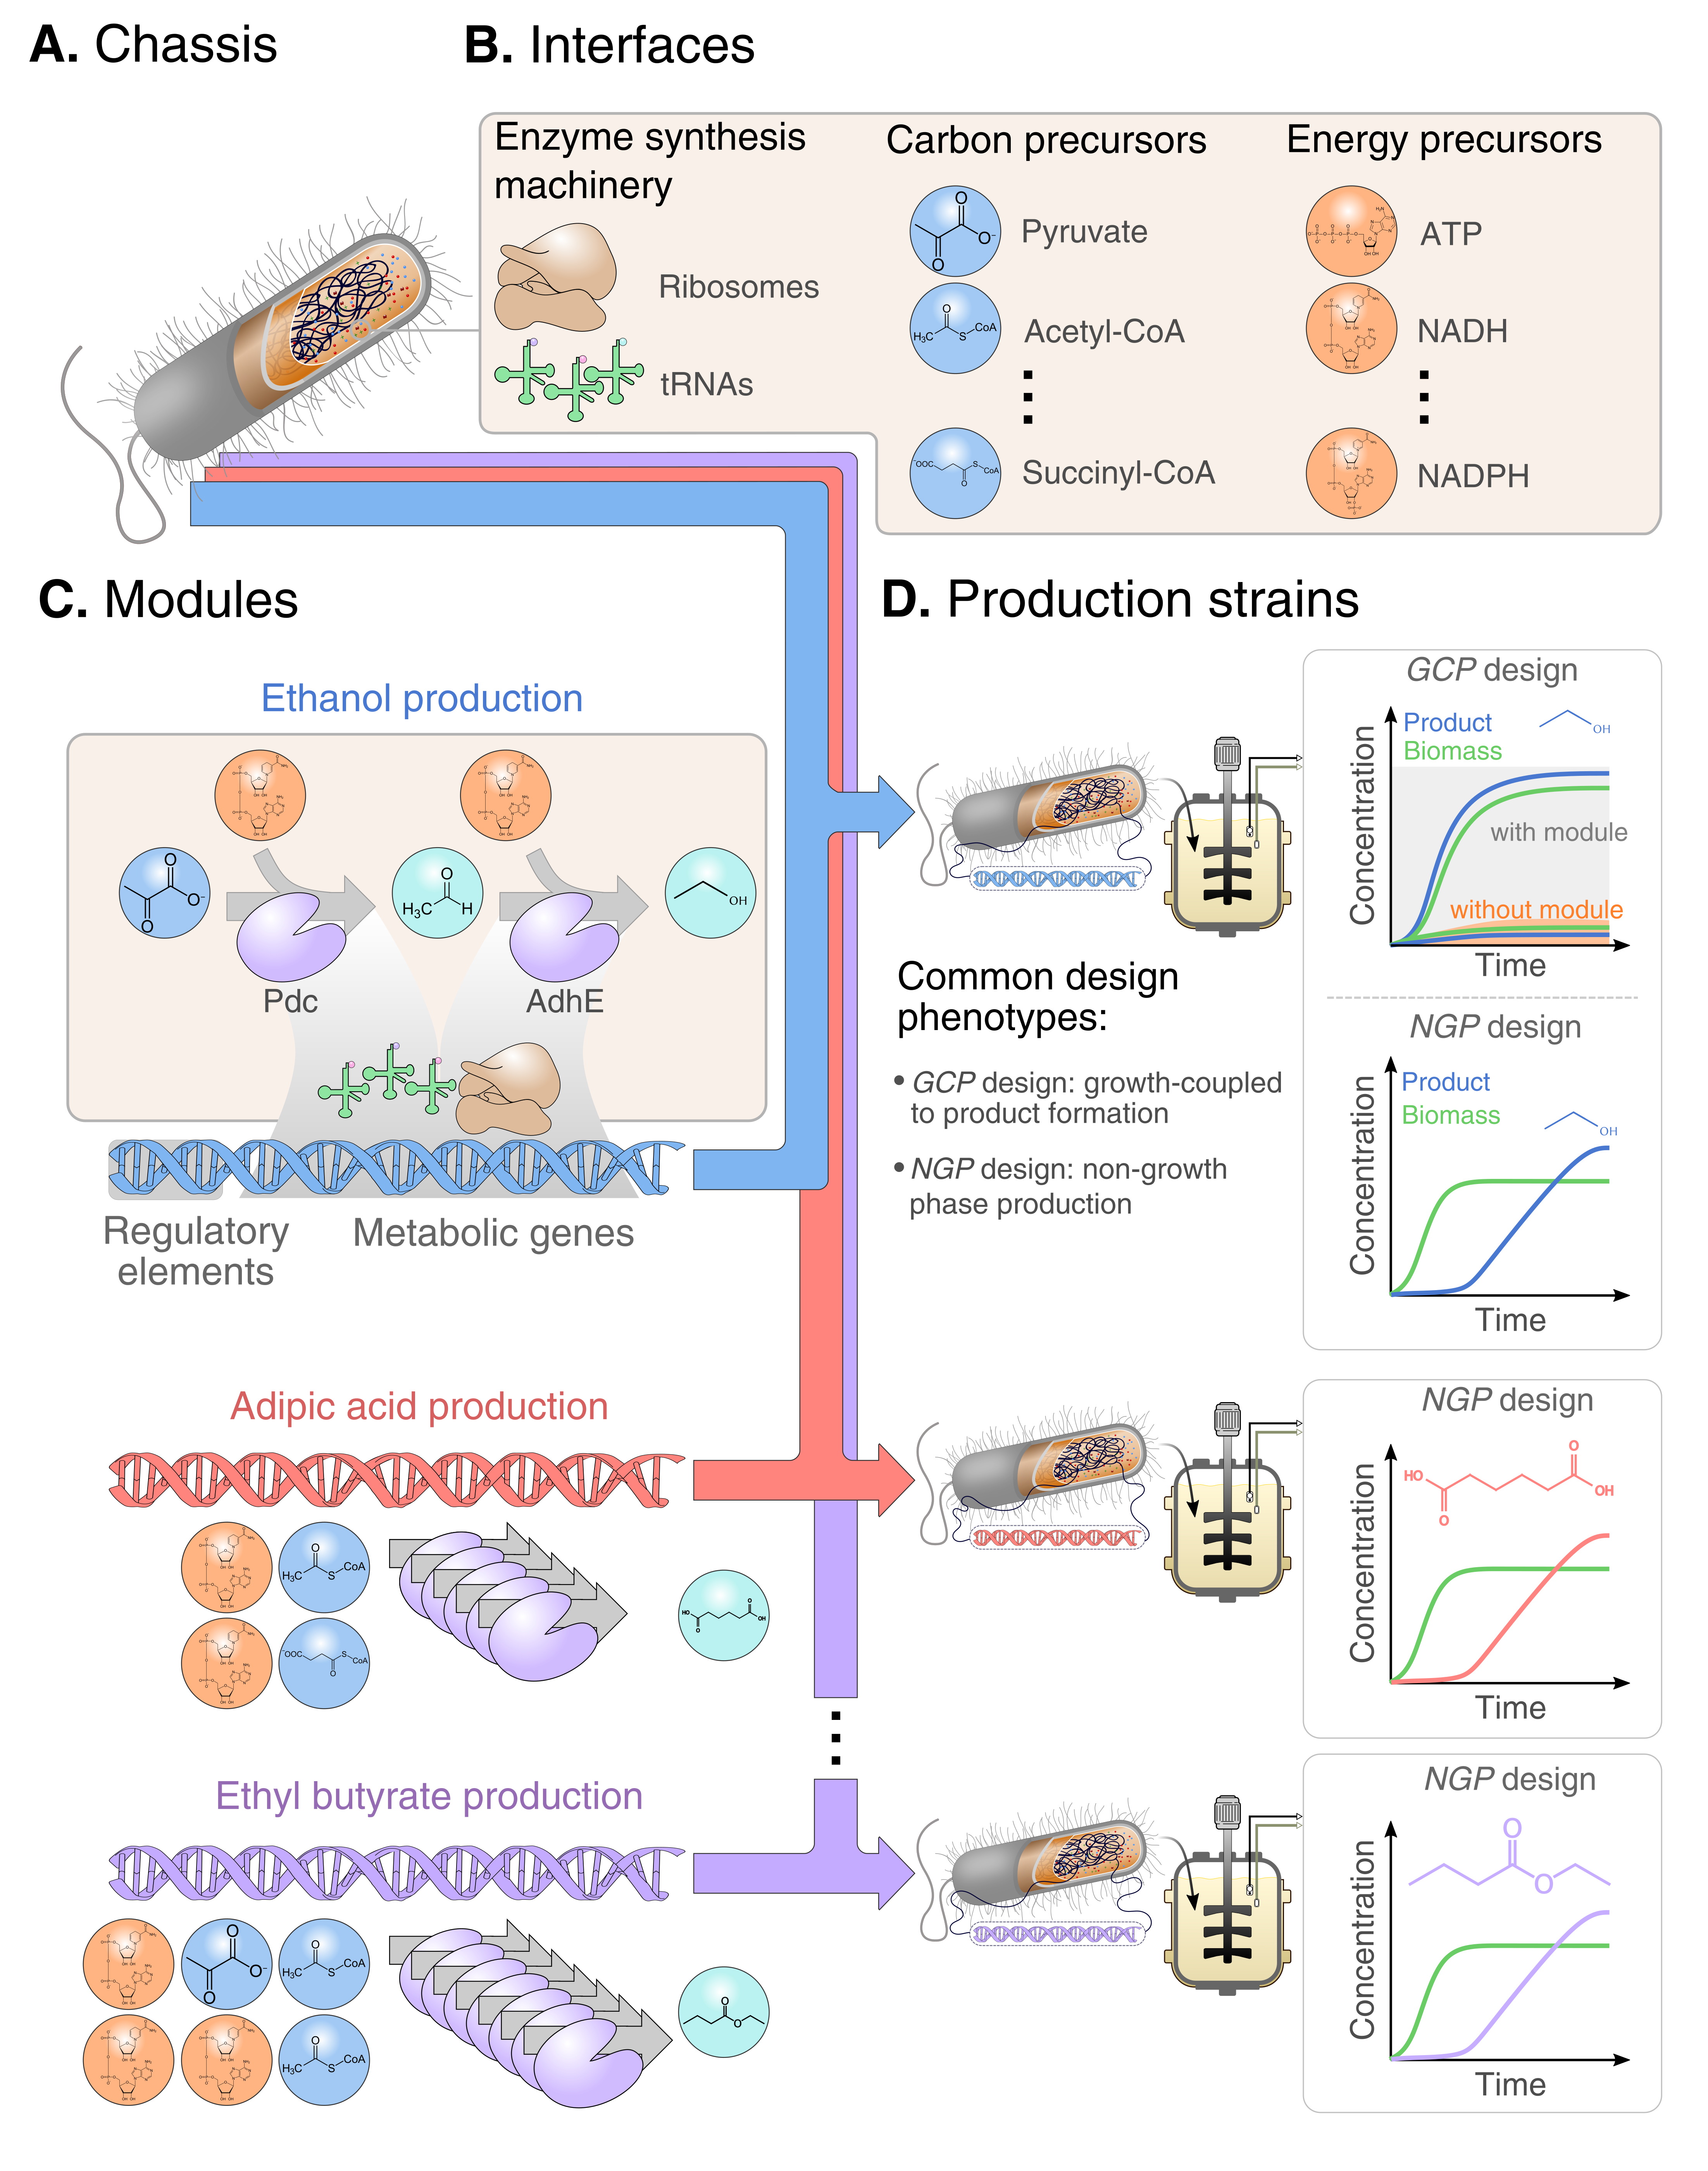
\includegraphics[width=\textwidth]{ba-fig3}
    \caption[Generalized concept of modular cell design]{Generalized concept of modular cell design.
    (\textbf{A}) Modular (chassis) cell. \textbf{(B)} Interfaces.
(\textbf{C}) Production modules. \textbf{(D)} Production strains. A
modular cell is designed to provide the necessary precursors for
biosynthesis pathway modules that are independently assembled with the
modular cell to generate production strains exhibiting desirable
phenotypes.}
    \label{fig:ba-fig3}
\end{figure}
%}

\subsection{Recent developments in mathematical formulation of modular cell design}


The primer for the modular cell design principles started with the observation \citep{trinh2012} that the optimal design of the n-butanol- and isobutanol-producing \emph{E.
coli} cells\emph{,} based on constraint-based modeling \citep{palsson2015} and conventional strain design methods \citep{trinh2009}, exhibited the same core metabolism (Figure~\ref{fig:ba-fig4}~A-B).
To systematically explore this property, the first modular cell design method, called MODCELL, was proposed and used to design an \emph{E.
coli} modular cell for alcohol and ester production \citep{trinh2015} (Figure~\ref{fig:ba-fig4}~E).
In Chapter~\ref{ch:modcell2} a new formulation of the modular cell design problem, ModCell2, based on multi-objective optimization will be developed to design strains with minimal trade-off between compatibility, performance, and robustness (Figure~\ref{fig:ba-fig4}~H).

%A new formulation of the modular cell design problem, ModCell2 \citep{garcia2019}, was proposed based on the framework of multi-objective optimization to capture the tradeoffs that may exist among highly diverse biochemical pathways.
%ModCell2 enables analysis of genome-scale metabolic networks with many production modules and design of optimal modules without extensive prior knowledge of target pathways.
%ModCell2 was used to demonstrate that a modular cell can be designed to exhibit (i) desirable production phenotypes for many molecules under various culturing conditions beyond the growth-coupled to product synthesis phase \citep{klamt2015}, such as the stationary-phase phase \citep{klamt2018}, and (ii) minimal trade-off between compatibility, performance, and robustness (Figure~\ref{fig:ba-fig4}~H).
%These results highlight that the systems-level modularization of cellular metabolism can accelerate strain engineering without sacrificing performance requirements.

While ModCell2 is to our knowledge the only tool that involves simultaneous design of chassis, modules, and interfaces, other recently developed computational tools can be applied to design these elements individually.
For example, MinGenome \citep{wang2018} is used to design genomes of minimal cells that can serve as chassis whereas ValveFind \citep{pandit2017} enables design of orthogonal pathways to build production modules.
Topics on model-guided strain design techniques for ``integral'' strains, .i.e, strains optimized for production of only a single product, can be found in recent excellent reviews.
\citep{long2015, machado2015, ng2015}.

Future development of modular cell design tools will incorporate enzyme kinetics of cellular metabolism \citep{king2015, noor2016} to account for potential metabolic burdens \citep{wu2016} in the design of modular cells and exchangeable production modules (Figure~\ref{fig:ba-fig4}~I).
Enzyme cost analysis is also particularly useful for identifying robust strategies for adaptive laboratory evolution that prevent an unintended pathway(s) to be optimized instead of a targeted pathway(s) \citep{dinh2018}.
The lack of experimental data on enzyme catalytic efficiencies needed for these modeling approaches can be addressed through random parameter sampling \citep{dinh2018}, \emph{omics} integration \citep{ebrahim2016, khodayari2016}, and machine learning \citep{heckmann2018}.
Recently developed models that predict \emph{in-vivo} enzyme concentrations from the genetic sequence help bridge the gap between metabolic model predictions and experimental implementation \citep{farasat2014, meng2013, salis2009}.

%\afterpage{
%\begin{figure}[H]
\begin{figure}[!p]
  \centering
  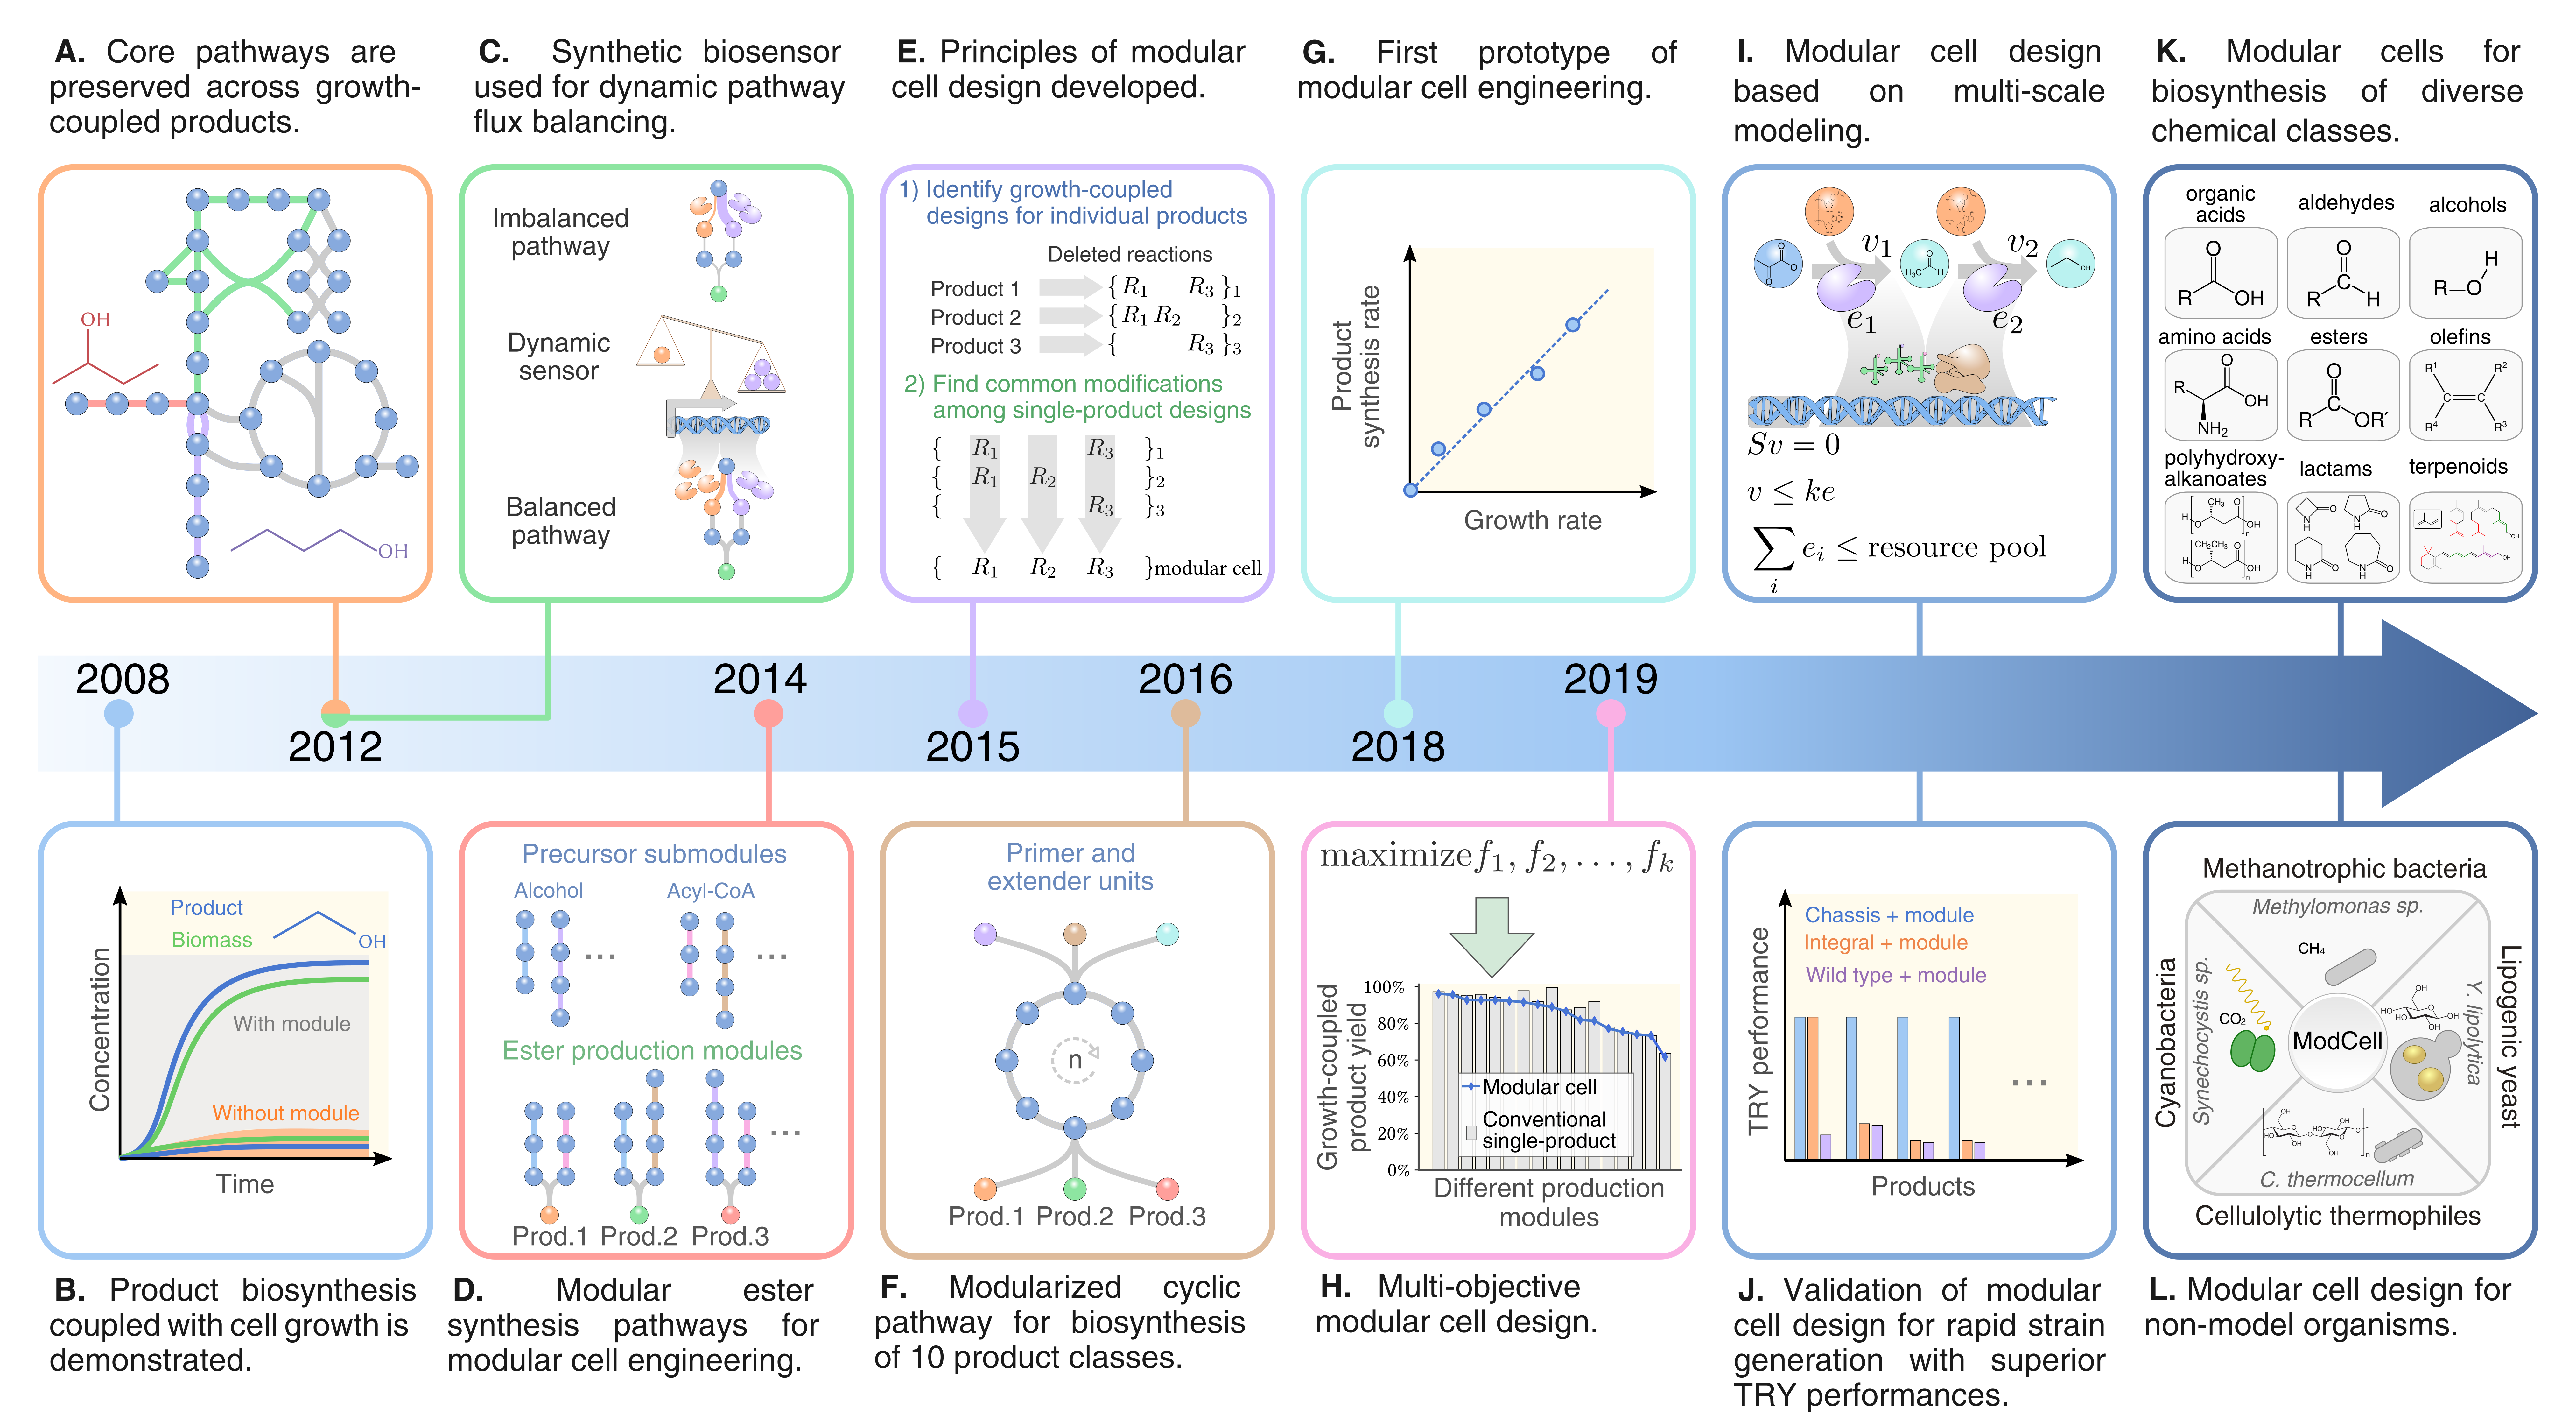
\includegraphics[width=\textwidth]{ba-fig4}
    \caption[Key advances and opportunities in the design and
    implementation of modular cells and exchangeable production modules]{Key advances and opportunities in the design and
implementation of modular cells and exchangeable production modules.
    (\textbf{A}) The same core metabolic pathways were revealed for butanol
and isobutanol growth-coupled production based on elementary mode
analysis \citep{trinh2012}. (\textbf{B}) An \emph{E. coli}
cell with minimal metabolic functionality designed to require product
(ethanol) synthesis for cell growth was experimentally validated
\citep{trinh2008}. (\textbf{C}) A dynamic sensor-regulator
system was designed and implemented to balance metabolic fluxes for
enhanced biosynthesis of fatty acid-derived molecules
\citep{zhang2012}. (\textbf{D}) A modular ester fermentative
pathway platform derived from alcohol and acyl-CoA pathway submodules
was designed and experimentally demonstrated in a chassis strain
\citep{layton2014}. (\textbf{E}) First modular cell design
method, named MODCELL, was proposed and used to design 3 modular cells
for the production of a group of alcohols and derived esters
\citep{trinh2015}. (\textbf{F}). Carbon and energy efficient
cyclic pathway was developed to synthesize 10 product classes from a
variety of primer and extender precursors \citep{cheong2016}.
(\textbf{G}) Prototypes of modular cell engineering were demonstrated
for growth-coupled to product synthesis predicted by MODCELL
\citep{trinh2015} and pathway optimization by adaptive
laboratory evolution \citep{wilbanks2017}. (\textbf{H})
Multi-objective optimization-based modular cell design method, named
ModCell2, will be developed in Chapter~\ref{ch:modcell2} and used to reveal negligible trade-offs
between modular and integral designs.
(\textbf{I}) Next-generation of modular cell design framework is
proposed to account for enzyme biosynthesis cost using metabolism and
expression (ME) or kinetic models with enzyme constraints. (\textbf{J})
Experimental demonstration of rapid and systematic generation of modular
production strains with many different types of production modules to
achieve superior performances over the wildtype and single-product
(integral) strains in terms of titer, rate, and yield (TRY).
(\textbf{K}) Design of a universal modular cell compatible with a large
and diverse space of production modules. (\textbf{L}) Future
demonstration of modular cell design is proposed for
industrially-relevant, non-model organisms with difficult-to-transfer
phenotypes, such as efficient assimilation of CO\textsubscript{2},
    CH\textsubscript{4}, or cellulose.}
    \label{fig:ba-fig4}
\end{figure}
%}

\subsection{Recent advances in discovery and optimization of metabolic pathways as production modules}

With the arrival of quantitative `omics era in mid 1990s, we started to gain a deeper understanding of complex biological systems and categorize them into the functional biological parts, i.e., regulatory and functional genes for retrieval through development of biological databases (e.g., Registry of Standard Biological Parts (https://parts.igem.org), KEGG \citep{kanehisa2000}, Biocyc \citep{caspi2013}, Brenda \citep{scheer2010}, among many others).
Synergistically, the interdisciplinary areas of bioinformatics, synthetic biology, metabolic and protein engineering have also emerged, advanced, and now enabled rapid and systematic identification and assembly of these biological parts into production modules to probe a large space of molecules that are only limited by one's imagination.
Nowadays, development of production modules can start by using computational tools with increasing scope and accuracy \citep{kumar2018, wang2017}, that help identify metabolic steps, associated enzymes, and genetic parts (i.e., promoters, terminators, ribosome binding sites, regulatory/sensory elements, and so on) using a combination of elementary reaction rules, yield, thermodynamic, and biophysical analyses \citep{dugar2011, kumar2018}.
Next, the genetic parts can be synthesized, assembled, and characterized for accuracy in a rapid manner to build production modules to make desirable molecules in a target host \citep{annaluru2014, bitinaite2007, blake2010, chen2013, colloms2014, gibson2009, kok2014, li2005, li2007, shao2009, trubitsyna2014, tsuge2003, zhang2012b}.
Some recent achievements, highlighting innovations in retrofitting cellular metabolism for novel biocatalysis from sustainable feedstocks, include: (i) redirection of central metabolism to make environmentally friendly, non-natural bioplastics \citep{rehm2010}, (ii) redesign of fermentative pathways to produce a large space of designer bioesters used as flavors, fragrances, biofuels, and solvents \citep{layton2014, rodriguez2014} (Figure~\ref{fig:ba-fig4}~D), (iii) repurposing of the beta-oxidation pathway for combinatorial biosynthesis of alcohols, dicarboxylic acids, hydroxyl acids, and lactones as industrial platform chemicals \citep{cheong2016} (Figure~\ref{fig:ba-fig4}~F), and (iv) refactoring of polyketide and isoprenoid pathways to explore a large space of secondary metabolites as drugs \citep{ajikumar2010, galanie2015, martin2003}.

While the design, construction, and characterization of production modules can be streamlined, compatibility between the modules and a target host has always posed a significant challenge mainly due to the intricate flux imbalance resulting in low product titers, rates, and yields \citep{nielsen2016}.
In the case of heterologous enzyme expression, undesirable regulatory interactions at the transcriptional and metabolic levels might hinder the pathway operation in a new host.
This problem can be addressed by refactoring pathways into isolated orthogonal modules that are independent of the source organism regulation and do not interfere with heterologous host regulation \citep{galanie2015, RN171, tan2017, temme2012}.
In most design scenarios, even after regulatory issues are addressed, metabolic flux imbalance is likely to occur due to the differences in expression and catalytic efficiencies of pathway enzymes.
Metabolic flux balancing of engineered pathways is a combinatorial optimization problem that requires modification of gene expression elements (e.g., promoters, ribosome binding sites, etc.) and enzyme engineering to achieve the desired fluxes.
Currently, this combinatorial problem is often tackled in two ways: (i) identification of key design variables and screening and (ii) pathway selection.
The search space in variable screening approaches can be reduced by pathway-level modularization, known as Multivariate Modular Metabolic Engineering \citep{biggs2014, jeschek2017, yadav2012}.
Screening approaches can be effort-intensive and impractical for certain scenarios due to the extensive strain characterizations required to effectively sample the design space.
Additionally, these approaches may not be able to solve poor pathway-host interactions where precursor metabolite(s) of the pathway of interest becomes the bottleneck.
Alternatively, simultaneous host and pathway optimization can be accomplished by adaptive laboratory evolution, provided that a simple selectable phenotype such as growth is tightly coupled with the desirable product synthesis phenotype.
For example, Wilbanks \emph{et al.} \citep{wilbanks2017} recently demonstrated a linear correlation between growth rate and product synthesis rate for computationally designed growth-coupled strains \citep{trinh2015} (Figure~\ref{fig:ba-fig4}~G).
Pathway optimization through growth-coupled design has been applied successfully \citep{fong2005}, and a recent computational study suggest its applicability to many different products and organisms. \citep{von2017}
Modular cell design is compatible with the two described module optimization tools; particularly, the design of a chassis growth-coupled to its production modules can enable rapid optimization of diverse pathways.

\subsection{Recent advances in the experimental implementation of modular cell design}

Experimental implementation of modular cell design is still at infancy of validation.
Construction of modular cells can be implemented by two methods: (i) top-down approach that aims to remove undesired phenotypes from a naturally existing organism under defined environmental conditions \citep{trinh2008, trinh2006} and (ii) bottom-up approach that seeks to create a new organism derived from a synthetic minimal cell.
\citep{hutchison2016} These two methods draw the same analogy as those in the engineering modular design, classified as ``product modularization'' and ``design with modules'' \citep{bonvoisin2016}.
In the ``product modularization'' approach like the ``top-down'' approach, the chassis, modules, and interfaces are simultaneously designed either by defining functional carriers and interfaces as part of the design (\emph{ex ante} design) or by clustering existing functions into modules (\emph{ex post} design).
Alternatively, in the ``design with modules'' approach like the ``bottom-up'' approach, a product is designed out of a collection of predefined compatible parts; for example, the design of a personal computer that is assembled from the existing modules, including a motherboard, a graphic card, a monitor, etc., with standard interfaces.
In the modular cell design context, a minimal cell can function as chassis whereas orthogonal refactored pathways that function as modules are independently designed and combined with the chassis to build modular production strains with desirable phenotypes.

To date, all recent computational \citep{garcia2019, trinh2015} and experimental \citep{layton2014, wilbanks2017} efforts in implementing modular cell design have been focused on the top-down approach, since it is more feasible and accessible with the current knowledge and available genetic tools.
Even though the bottom-up approach is much more challenging \citep{hutchison2016}, the design principles developed for top-down construction can be applied to create bottom-up minimal modular cells, which would be less prone to failure due to their simpler architecture.
Regardless of which approach is chosen, the underlying genotypes essential to target product synthesis appear to be conserved, according to the recent surveys of over two decades of metabolic engineering reports \citep{king2017, winkler2015}.
This suggests that modular cell design can serve as a unifying platform for rapid strain engineering (Figure~\ref{fig:ba-fig4}~J).

An anticipated challenge of modular cell design is that the chassis must provide enough precursor metabolites and enzyme synthesis machinery to support the target flux through each module.
This issue may become increasingly difficult as the biochemical diversity and number of products supported by a single chassis expands (Figure~\ref{fig:ba-fig4}~K).
Recent developments in biosensors coupled with gene expression regulation tools \citep{liu2015, meyer2018, moser2018, yang2018, zhang2012} can achieve tunable control over the host metabolism to meet the requirements of each production module (Figure~\ref{fig:ba-fig4}~C).
In practice, such regulatory elements may be implemented in the host or as a part of specific modules.

\section{Conclusions}

Inspired by natural and conventional engineering modularity, bioengineers have started applying modular design principles to engineer biological systems at genetic, enzymatic, and cellular levels.
Modular cell design aims to integrate all three levels for rapidly creating novel microbial biocatalysts in a plug-and-play fashion with minimal strain optimization cycles.
Advancements in genome reading \citep{goodwin2016}, writing \citep{casini2015, kosuri2014}, and editing \citep{barrangou2016} will provide a unique opportunity to streamline modular cell engineering that effectively harnesses a large space of molecules from cellular metabolism using single organisms or microbial consortia, especially from non-model organisms with industrially-relevant but not-easy-to-transfer traits (Figure~\ref{fig:ba-fig4}~L) \citep{abdel-mawgoud2018, carroll2018, kalyuzhnaya2015, lynd2016, thompson2016}.
Particularly, these advancements help streamline the construction of modular cells and exchangeable production modules from both top-down and bottom-up approaches.
To further advance modular cell engineering, it is important not only to optimize the interfaces between production modules and modular cell but also to account for robustness and evolvability towards desirable engineered phenotypes.
By combining proven engineering methods rooted in the physical and chemical laws with system modeling frameworks (e.g., Pareto optimality theory, graph theory), we can elucidate the modular design principles in biology from natural systems to engineered ones, leading towards fundamental understanding of essential rules of life and broader industrialization of biology.

%\textbf{Acknowledgements}
%
%This research was financially supported in part by a NSF CAREER award (NSF\#1553250), a DOE BER Genomic Science Program award (DE-SC0019412), and The Center for Bioenergy Innovation (CBI), the U.S.
%Department of Energy (DOE) Bioenergy Research Centers funded by the Office of Biological and Environmental Research in the DOE Office of Science.
%Due to space limitation, we sincerely apologize to those whose work was not cited.







    \chapter{Formulation of conceptual and mathematical framework to design modular cells}\label{ch:modcell2}
% Metabolic engineering paper

\disclose{Multiobjective strain design: A framework for modular cell engineering. Garcia, S., and Trinh, C. T. Metabolic Engineering, 2019}%{garcia2019}
Supplementary Files S1 and S2 are provided in Appendix \ref{apx:sm1-modcell2} and \ref{apx:sm2-modcell2} respectively, while Supplementary Files S3, S4, and S5 are provided as attachments.


\section*{Abstract}\label{abstract}

Diversity of cellular metabolism can be harnessed to produce a large space of molecules.
However, development of optimal strains with high product titers, rates, and yields required for industrial production is laborious and expensive.
To accelerate the strain engineering process, we have recently introduced a modular cell design concept that enables rapid generation of optimal production strains by systematically assembling a modular cell with an exchangeable production module(s) to produce target molecules efficiently.
In this study, we formulated the modular cell design concept as a general multi-objective optimization problem with flexible design objectives derived from mass action.
We developed algorithms and an associated software package, named ModCell2 to implement the design.
We demonstrated that ModCell2 can systematically identify genetic modifications to design modular cells that can couple with a variety of production modules and exhibit a minimal tradeoff among modularity, performance, and robustness.
Analysis of the modular cell designs revealed both intuitive and complex metabolic architectures enabling modular production of these molecules.
We envision ModCell2 provides a powerful tool to guide modular cell engineering and sheds light on modular design principles of biological systems.

%\section{Keywords}\label{keywords}
%
%Modular cell engineering; modular cell; production modules; modular design; modularity; multi-objective optimization; multi-objective evolutionary algorithms.
%

\section{Introduction}

Engineering microbial cells to produce bulk and specialty chemicals from renewable and sustainable feedstocks is becoming a feasible alternative to traditional chemical methods that rely on petroleum feedstocks \citep{nielsen2016}.
However, only a handful of chemicals, out of the many possible molecules offered by nature, are industrially produced by microbial conversion, mainly because the current strain engineering process is laborious and expensive for profitable biochemical production \citep{trinh2016}.
Thus, innovative technologies to enable rapid and economical strain engineering are needed to harness a large space of industrially-relevant molecules \citep{connelly2015}.

The modular organization of biological systems has been a source of inspiration for synthetic biology and metabolic engineering \citep{purnick2009, sauro2008}.
Modular pathway engineering breaks down target pathways into tractable pathway modules that can be finely tuned for optimal production of desirable chemicals \citep{biggs2014, yadav2012}.
Harnessing combinatorial pathways (e.g., fatty acid biosynthesis, reverse beta oxidation, polyketide or isoprenoid biosynthesis) is one excellent example of modular pathway engineering.
These pathways contain metabolic similarity (or combinatorial characteristics) such as a group of common specific enzymes capable of catalyzing linear reaction steps \citep{rodriguez2014} and/or elongation cycles \citep{cheong2016, tseng2012, xu2013} and hence are capable of producing a large library of unique molecules \citep{ng2016}.
Since these molecules are derived from a common precursor metabolite(s), the optimal production strains often share common genotypes and phenotypes, and hence, the costly strain optimization process is only performed once for these molecules.
Remarkably, this advantageous strain optimization strategy can be applied even for production of molecules derived from different precursors, using the concept of modular cell (ModCell) design \citep{trinh2015, trinh2016, wilbanks2017}.

With the arrival of steady-state, constraint-based stoichiometric models of cellular metabolism, various computational algorithms have been developed to guide strain engineering \citep{chowdhury2015, long2015, yang2011}.
These methods have featured the design of strains capable of growth-coupled product synthesis (\emph{GCP}), enabling adaptive laboratory evolution of these designed strains to enhance product titers, rates, and yields \citep{fong2005, yadav2012, trinh2009, wilbanks2017}.
Two approaches on growth-coupled production have been formulated - one based on the coexistence of maximum growth and product synthesis rates during the growth phase \citep{burgard2003} and the other based on the obligate requirement of optimal product synthesis in any growth phase \citep{trinh2008}.
The distinction between these two types of growth coupling are also referred to weak coupling (\emph{wGCP}) and strong coupling (\emph{sGCP}) \citep{klamt2015, yang2011}.

Development of most strain design algorithms has been focused on overproduction of only one target molecule.
The first algorithm proposed for modular cell design compatible for overproduction of multiple target molecules is MODCELL \citep{trinh2015}, which guided several experimental studies \citep{layton2016, layton2014, layton2016b, wierzbicki2016, wilbanks2017}.
It works by generating \emph{sGCP} strain designs for each target product based on elementary mode analysis \citep{trinh2009b}, and then comparing the design strategies of different products to identify common genetic modifications among them.
A similar approach was adapted in a subsequent work \citep{jouhten2016}.
For MODCELL to find optimal solutions for multiple target products, it requires: 1) enumerating all possible designs above a predefined minimum product yield and with minimal reaction deletion sets for each production network, which might lead to a large number of solutions for each network and hence make the problem computationally intractable, and 2) the resulting designs for all products must be compared to identify common interventions, which is a computationally-hard, set-covering problem.
Thus, the current enumerative approach of MODCELL might become intractable very quickly, especially for large-scale metabolic networks and potentially generate non-optimal designs, i.e., requiring more knock-outs than necessary or including fewer products than possible.

In this study, we generalized the concept of modular cell design and addressed the computational limitation of implementing it.
We developed a novel computational platform (ModCell2), based on multi-objective optimization and analysis of mass action of cellular metabolism, to guide the design of modular cells for large-scale metabolic networks.
We demonstrated that ModCell2 can systematically identify genetic modifications to design modular cells that can couple with a variety of production modules and exhibit a minimal tradeoff among modularity, performance, and robustness.
By analyzing these designs, we further revealed both intuitive and complex metabolic architectures enabling modularity in modular cell and production modules required for efficient biosynthesis of target molecules.


\section{Methods}

\subsection{Design principles of modular cell
engineering}

In the conventional strain engineering approach, a parent strain is genetically modified to yield an optimal production strain to make only a target product.
To produce each new molecule, the design-build-test cycles of strain engineering must be repeated, which is laborious and expensive (Figure~\ref{fig:ms1-fig1}).
To minimize the cycles, modular cell engineering is formulated by genetically transforming a parent strain into a modular (chassis) cell that must be assembled with exchangeable modules to create optimal production strains \citep{trinh2015}.
A modular cell is designed to contain core metabolic pathways shared across designed optimal production strains.
Exchangeable modules are production pathways designed to synthesize desirable chemicals.
A combination of a modular cell and a production module(s) is required to balance redox, energy, and precursor metabolites for sustaining cellular metabolism during growth and/or stationary phases and exhibiting only desirable phenotypes.
Practically, modular cell engineering can be applied to monocultures and polycultures, where a production module(s) can be embedded in a modular cell and activated by intracellular and/or extracellular cues such as light and/or signaling molecules.

\begin{figure}[h]
  \centering
  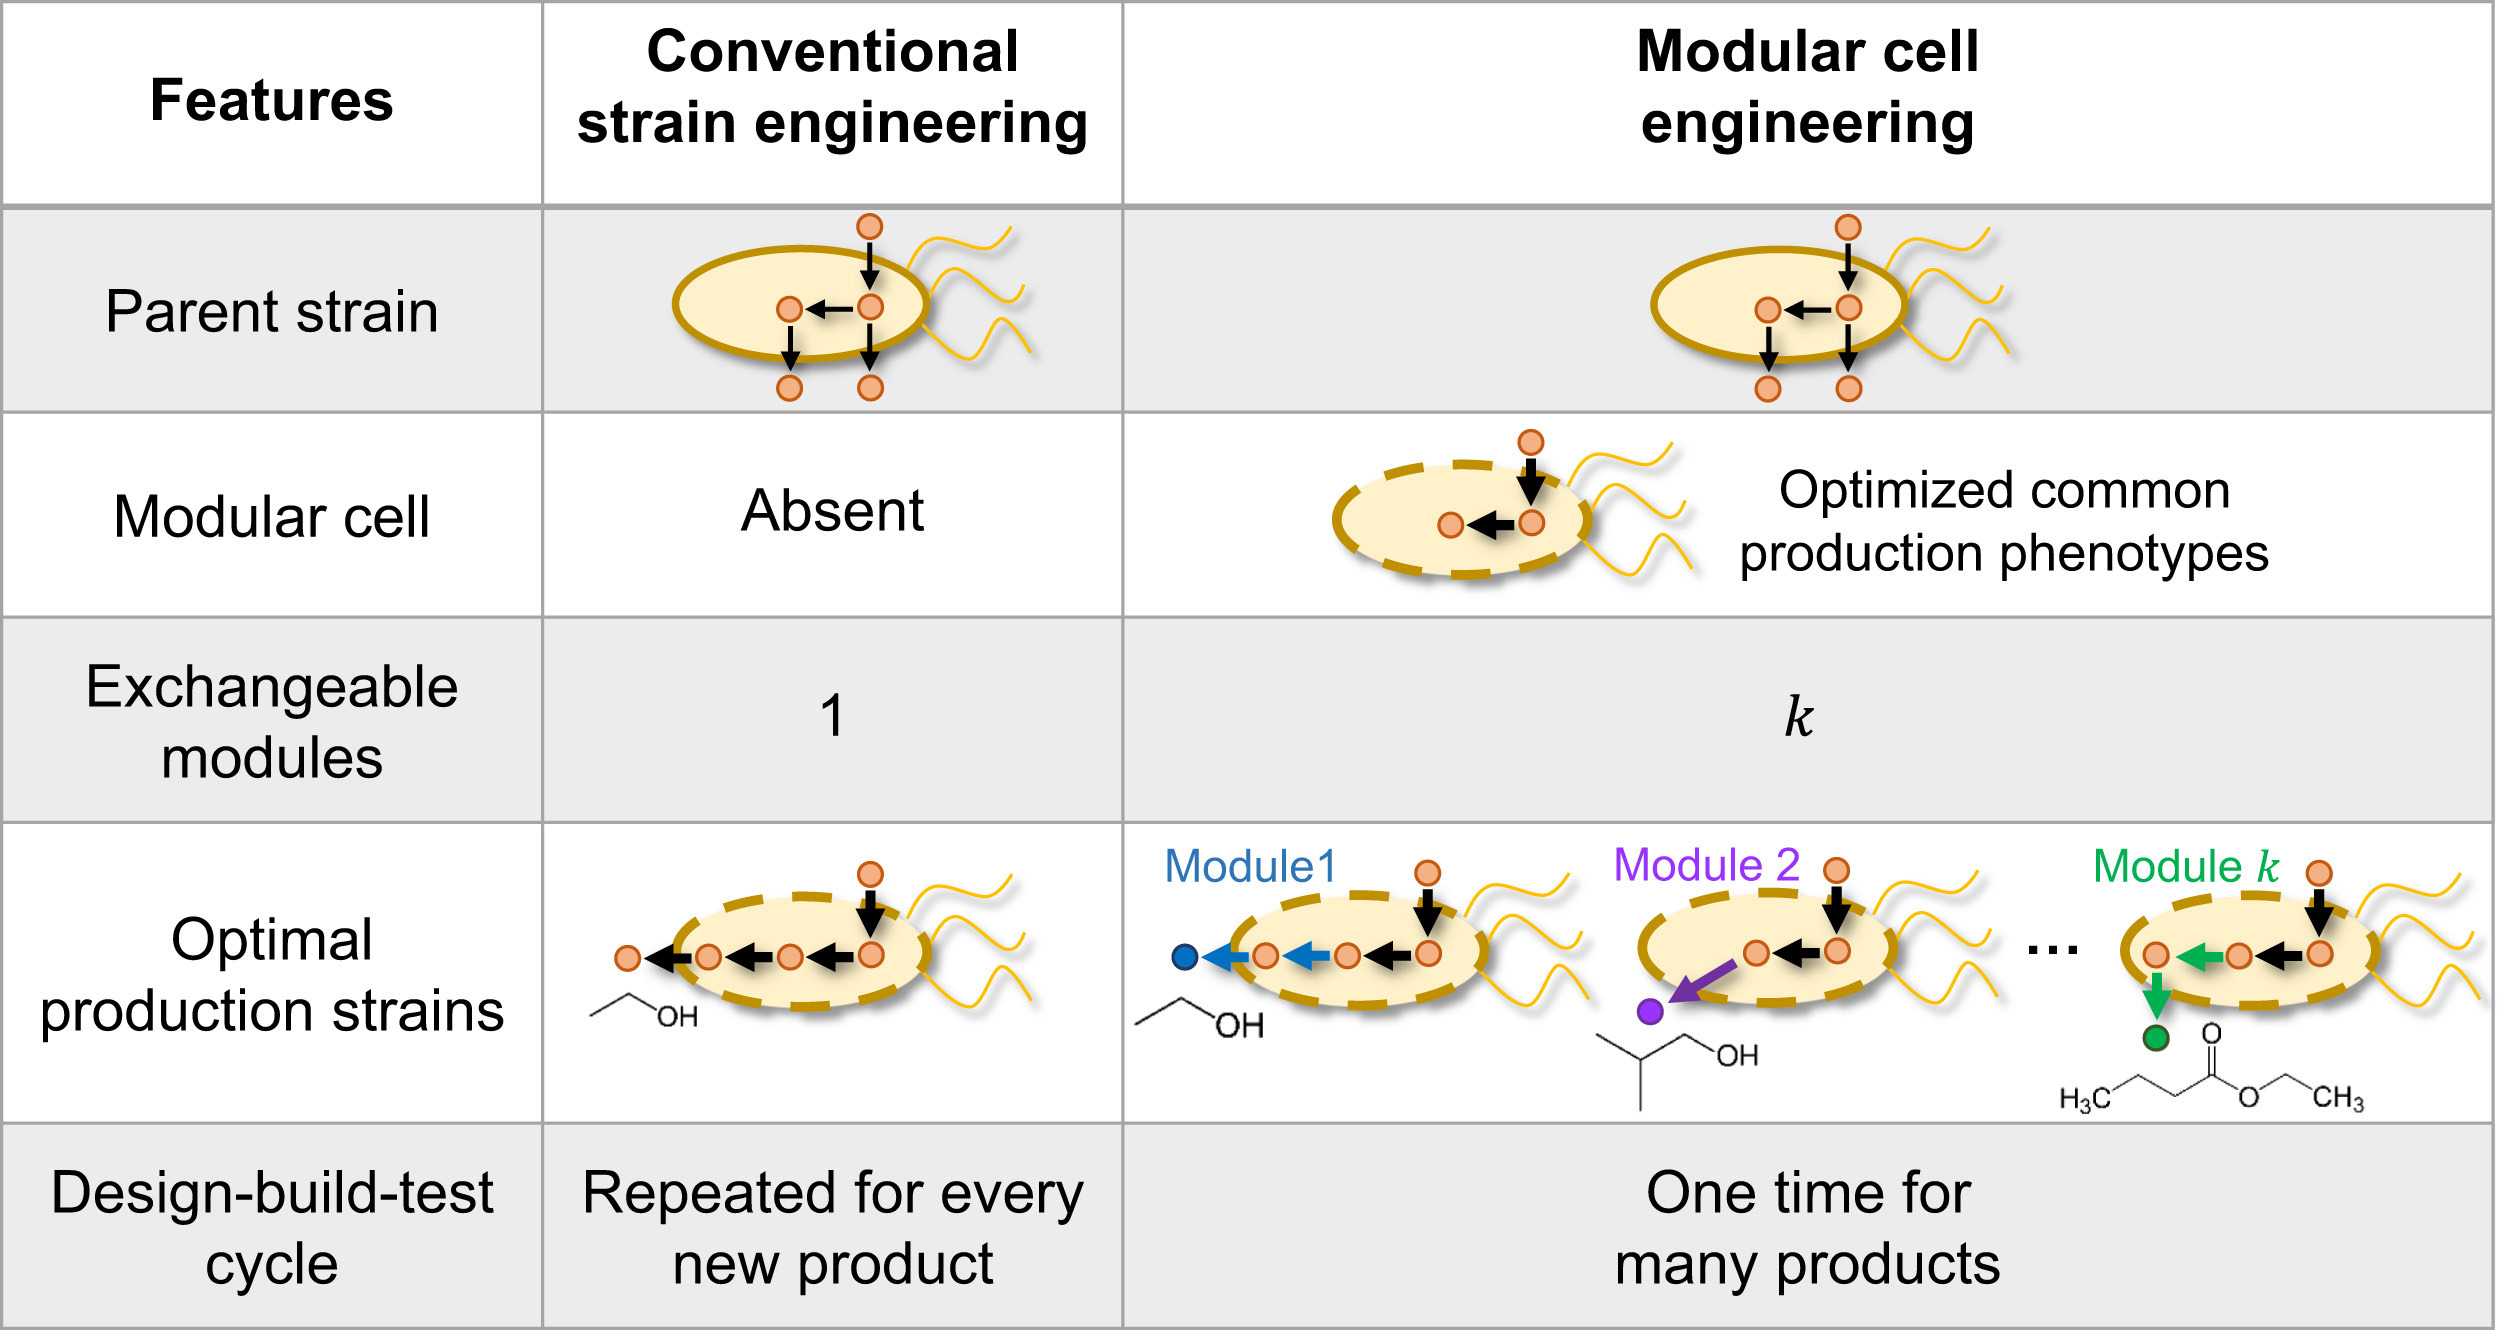
\includegraphics[width=\textwidth]{ms1-1}
    \caption[Comparison between the conventional single-product strain design and modular cell engineering]{
Comparison between the conventional single-product
strain design and modular cell engineering. In the conventional
approach, each target product requires to go through the iterative
optimization cycle. The modular cell engineering approach exploits
common phenotypes associated with high product titers, rates, and
yields; and hence, the strain optimization cycle only needs to be
performed once for multiple products, which helps reduce the cost and
time of strain development.
    }
    \label{fig:ms1-fig1}
\end{figure}

\subsection{Multi-objective strain design framework for modular cell engineering}

For modular cell engineering, we seek to design a chassis cell compatible with as many production modules as possible to achieve only desirable production phenotypes while requiring minimal genetic modifications.
Since all production modules must leverage cellular resources of the modular cell (e.g.
precursor metabolites, cofactors, and energy), they form competing objectives.
Therefore, the framework of modular cell engineering can be formulated as a multi-objective optimization problem, named ModCell2, as described below.

\begin{alignat}{3}
    & \underset{ \; y_j, z_{jk}}{\textrm{maximize}} \quad (f_1, f_2, \ldots, f_{|\mathcal{K}|})^T \quad \text{subject to}  \label{eq3:of1} \\
	&  \quad f_k \in \, \text{arg }\underset{}{\text{max}} \Bigg\{\sum_{j \in \mathcal{J}_k} c_{jk}  v_{jk} \quad \text{subject to} \label{eq3:of2}\\
	& \quad \qquad \sum_{j\in \mathcal{J}_k}S_{ijk}v_{jk} = 0 && \text{for all } i \in \mathcal{I}_k  \label{eq3:mb}\\
	& \quad \qquad  l_{jk} \le v_{jk} \le u_{jk}  && \text{for all } j \in \mathcal{J}_k \label{eq3:rb}\\
	& \quad \qquad  l_{jk} d_{jk} \le v_{jk} \le u_{jk} d_{jk} && \text{for all } j \in \mathcal{C} \label{eq3:db}\\
	& \quad \qquad \mathrm{where} \; d_{jk} = y_j \lor z_{jk} \; \Bigg\} && \text{for all } k \in \mathcal{K} \nonumber \\
	& \quad z_{jk}\le (1-y_j) && \text{for all } j \in \mathcal{C}, \, k \in \mathcal{K} \label{eq3:mr1}\\
	& \quad \sum_{j \in \mathcal{C}}z_{jk} \le \beta_k && \text{for all } k \in \mathcal{K} \label{eq3:mr2} \\
	& \quad \sum_{j \in \mathcal{C}} (1-y_j) \le \alpha \label{eq3:a}
\end{alignat}

\noindent where $i$, $j$, and $k$ are indices of metabolite $i$, reaction $j$, and production network $k$, respectively; $f_k$ is a design objective for network $k$; $c_{jk}$ represents the cellular objective for reaction $j$ in network $k$ associated with a design objective defined in (\ref{eq3:wgcp} -\ref{eq3:ngp}); $v_{jk}$ (mmol/g DCW/h) is metabolic flux of reaction $j$ bounded by $l_{jk}$ and $u_{jk}$ in network $k$, respectively; $y_j$ and $z_{jk}$ are binary design variables for deletion reaction $j$ and module reaction $j$ in network $k$, respectively; $\alpha$ and $\beta_k$ are design parameters for deletion and module reactions, respectively; $S_{ijk}$ is a stoichiometric coefficient of metabolite in reaction $j$ of network \emph{k}; and \emph{C} \eqref{eq3:db} is the candidate reaction set (Supplementary File S1).
The goal of the optimization problem is to simultaneously maximize all design objectives \emph{f\textsubscript{k}}.

\subsubsection{Steady-state mass balance constraint of cellular metabolism}
Quasi steady-state flux balance of cellular metabolism \eqref{eq3:mb} is used as metabolic constraints for \eqref{eq3:of1}.\citep{price2003}. A model corresponding to each modular
production strain (i.e. production network $k$) will be derived from a
parent strain (i.e. parent network) by adding necessary reactions (e.g.,
a production module) to produce a target molecule. A feasible flux
distribution for each production network is described by mass balance
\eqref{eq3:mb} and reaction flux bounds (\ref{eq3:rb}-\ref{eq3:db}). For a given
production network, the phenotypic space can be illustrated by the gray
area that is projected onto the two-dimensional space spanned by product
synthesis and growth rates (Figure~\ref{fig:ms1-fig2}).

\begin{figure}[h]
  \centering
  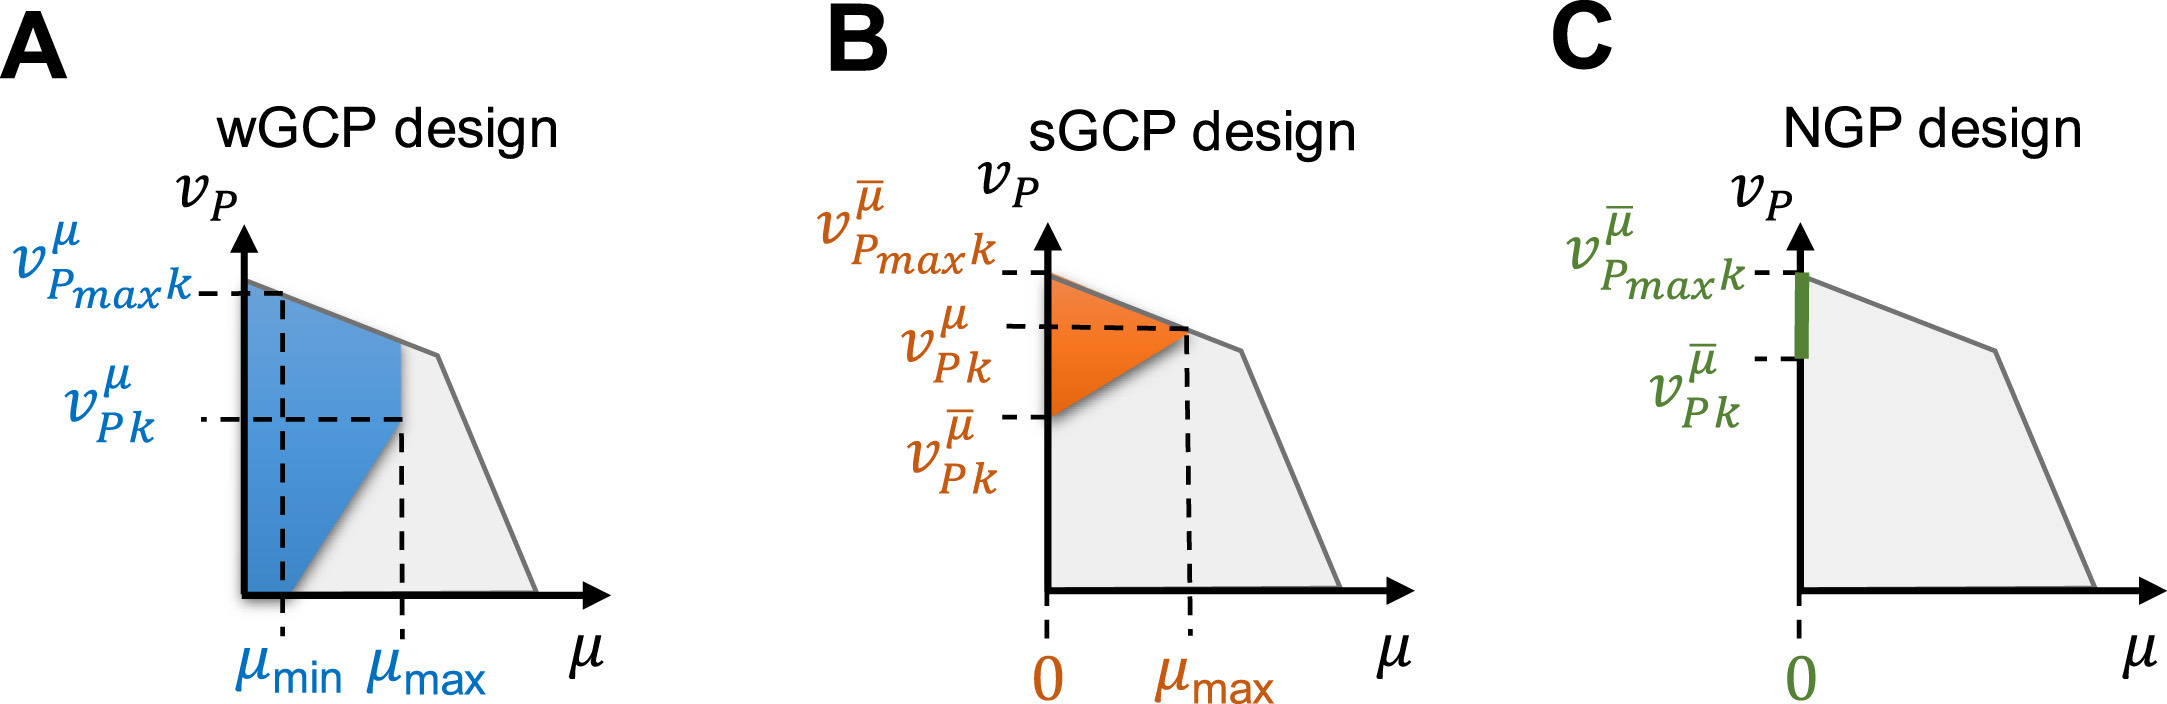
\includegraphics[width=\textwidth]{ms1-2}
    \caption[Graphical representation of phenotypic spaces for different strain design objectives]{
Graphical representation of phenotypic spaces for
different strain design objectives including \textbf{(A)} weak growth
coupling (\emph{wGCP}), \textbf{(B)} strong growth coupling
(\emph{sGCP}), and \textbf{(C)} no-growth production (\emph{NPG}).
\(v_{\text{Pk}}^{\mu}\) is the minimum product formation rate at the
maximum growth rate for production network \emph{k}, and
\(v_{P_{\max}k}^{\mu}\ \)is the maximum product secretion rate
attainable. \(v_{\text{Pk}}^{\overline{\mu}}\) and
\(v_{P_{\max}k}^{\overline{\mu}}\ \)are the minimum and maximum product
formation rates for production network \(k\) during the stationary
phase, respectively.
    }
    \label{fig:ms1-fig2}
\end{figure}

\subsubsection{Design variables} In our formulation for modular cell
engineering, we introduced two design variables: binary reaction
deletions (\emph{y\textsubscript{j}}) inherent to the modular cell and
module-specific reaction insertions (\emph{z\textsubscript{jk}}) \eqref{eq3:db}.
These variables can be experimentally manipulated to constrain the
desirable phenotypes of production strains as shown in Figure~\ref{fig:ms1-fig2}.
Specifically, \emph{y\textsubscript{j}} = 0 if reaction \emph{j} is
deleted from the modular cell; otherwise, \emph{y\textsubscript{j}} = 1.
Deleting metabolic reactions removes undesired functional states of the
network and leaves those with high design objectives. Likewise,
\emph{z\textsubscript{jk}} = 1 if reaction \emph{j} is present in the
production network \emph{k}; otherwise, \emph{z\textsubscript{jk}} = 0.
These module reactions are endogenous reactions removed from the parent
network \eqref{eq3:mr1} , but are added back to a specific production module to
enhance the compatibility of a modular cell. The maximum number of
reaction deletions ($\alpha$) and module-specific reaction insertions
($\beta_k$) are user-defined parameters.

\subsubsection{Design objectives} To generalize ModCell2 design, we allow
three different types of design objectives (\emph{f\textsubscript{k}},
\eqref{eq3:of1} that determine production phenotypes for each production
network. Depending on the application, a phenotype can be designed to be
weak coupling (\emph{wGCP}), strong coupling (\emph{sGCP}), and/or
non-growth production (\emph{NGP}) (Figure~\ref{fig:ms1-fig2}). The constrained
phenotypic spaces based on these design objectives are shown in color;
any point within these spaces is a feasible physiological state of the
cell that can be represented by a metabolic flux distribution.

The \emph{wGCP} design seeks to achieve a high product rate at maximum growth rate (Figure~\ref{fig:ms1-fig2}A).
The \emph{wGCP} design objective, $f_{k}^{\text{wGCP}} \in \{0, 1\}$, is calculated as follows:
\begin{equation}
    f_{k}^{\text{wGCP}} = \frac{v_{\text{Pk}}^{\mu}}{v_{\text{Pmaxk}}^{\mu}} \label{eq3:wgcp}
\end{equation}
\noindent where \(v_{\text{Pk}}^{\mu}\) is the minimum synthesis rate of the target product P at the maximum growth rate for production network \emph{k} and \(v_{\text{Pmaxk}}^{\mu}\) is the maximum synthesis rate of P (Supplementary File S1).
This \emph{wGCP} design formulation is equivalent to RobustKnock \citep{tepper2010} or OptKnock with a tilted objective function \citep{burgard2003, feist2010, yang2011}.
In \eqref{eq3:wgcp}, \(f_{k}^{\text{wGCP}}\) is scaled from 0 to 1 for proper comparison among products.
The \emph{wGCP} design is appropriate for applications where growth rate is not limited by the nutrients, and the product is formed during the growth phase.

The \emph{sGCP} design seeks to achieve a high product rate not only at optimal growth rate but also during non-growth phase (Figure~\ref{fig:ms1-fig2}B).
The \emph{sGCP} design objective,$f_{k}^{\text{sGCP}} \in \{0, 1\}$, is calculated as follows:

\begin{equation}
    f_{k}^{\text{sGCP}} = \frac{v_{\text{Pk}}^{\mu}}{v_{P_{\max}k}^{\mu}} \frac{v_{\text{Pk}}^{\overline{\mu}}}{v_{P_{\max}k}^{\overline{\mu}}} \label{eq3:sgcp}
\end{equation}
\noindent where \(v_{\text{Pk}}^{\overline{\mu}}\ \)and \(v_{P_{\max}k}^{\overline{\mu}}\ \)are the minimum and maximum product formation rates for production network \emph{k} in the stationary phase, respectively (Supplementary File S1).
The \emph{sGCP} design objective is comparable to the one implemented in MODCELL \citep{trinh2015}.
Different from \emph{wGCP}, \emph{sGCP} requires high product synthesis rate for any growth phase.
However, the additional constraint of optimal product synthesis during the stationary phase requires more genetic manipulations or specific experimental conditions (e.g., anaerobic growth condition, supply of intermediate metabolites).
Both \emph{wGCP} and \emph{sGCP} designs enable fast growth selection to attain the optimum product rates by adaptive laboratory evolution \citep{fong2005, trinh2009b}.

The \emph{NGP} design aims to maximize the minimum product rate during the non-growth phase by eliminating carbon fluxes directed to biomass synthesis (Figure~\ref{fig:ms1-fig2}C).
The \emph{NGP} design objective, $f_{k}^{\text{NGP}}\in \{0, 1\}$, is calculated as follows:

\begin{equation}
    f_{k}^{\text{NGP}} = \frac{v_{\text{Pk}}^{\overline{\mu}}}{v_{P_{\max}k}^{\overline{\mu}}} \label{eq3:ngp}
\end{equation}

While the \emph{NGP} design is not suitable for growth selection, it can be derived from a \emph{wGCP} (or \emph{sGCP}) design by imposing additional genetic modifications.
Practically, \emph{NGP} design strains can be activated during cell culturing using a regulatory genetic circuit to toggle switch between production phases.

\subsubsection{Design solutions}
Optimal solutions for (\ref{eq3:of1}-\ref{eq3:a} are a Pareto set
($\PS$) that correspond to design variables, including
reaction deletions (\emph{y\textsubscript{j}}) and module reaction
insertions (\emph{z\textsubscript{jk}}). Each solution constitutes a
design of a modular cell:

\begin{equation}
\PS = \{ x \in \Omega: \nexists t \in \Omega, \, F(t) \prec F(x) \}
\end{equation}
\noindent Here, \(\mathbf{F}\left( \mathbf{t} \right)\mathbf{\prec}\mathbf{F}\left( \mathbf{x} \right)\) means \textbf{F}(\textbf{t}) \emph{dominates} \textbf{F}(\textbf{x}) if and only if \(f_{i}\left( \mathbf{t} \right) \geq f_{i}\left( \mathbf{x} \right)\) for all \(i\), and \(\mathbf{F}\left( \mathbf{t} \right)\) differs from \(\mathbf{F}\left( \mathbf{x} \right)\) in at least one entry.
The feasible space of design variables, \(\Omega\), is defined by the problem constraints (\ref{eq3:of2}-\ref{eq3:a}), also see Supplementary File S1).
Phenotypes of modular cells will be the image of the Pareto set in the objective space, known as the Pareto front (\emph{\textbf{PF}}):
\begin{equation}
    \PF = \{ F(x):x \in \PS \}
\end{equation}

For the multi-objective strain design framework, the input parameters include $\alpha$ \eqref{eq3:a}, $\beta_k$ \eqref{eq3:mr3}
, and the production networks as input metabolic models.
Each model contains a production module to produce one target chemical.
The output is a Pareto set (genetic modifications) and its respective Pareto front (desirable production phenotypes).
For a special case with no trade-off among the design objectives, an optimal solution, named a utopia point, exists where each objective achieves its maximum value.
The multi-objective strain design formulation presented is general and can be applied to design modular cells for any organism.

\subsection{Algorithm and implementation}

\subsubsection{ModCell2 algorithm}
To solve the multi-objective
optimization problem for modular cell engineering, we used
multi-objective evolutionary algorithms (MOEAs)
\citep{coello2002}. MOEAs were selected because they can
efficiently handle linear and non-linear problems and do not require
preferential specification of design objectives
\citep{marler2004}. MOEAs start by randomly generating a
population of individuals (a vector of design variables), each of which
is mapped to a design objective vector (i.e., a fitness vector). In
ModCell2 (Supplementary File S1), the objective values of an individual
are calculated by solving the linear programming problems for each
production network. Next, individuals are shuffled to generate an
offspring, from which the most fit individuals are kept. This process
was repeated until the termination criteria was reached, for instance,
either the solutions cannot be further improved or the simulation time
limit is reached.

\subsubsection{ModCell2 implementation}
To streamline the modular cell
design, we developed the ModCell2 software package based on three core
classes (Figure S1 in Supplementary File S2). The Prodnet class parses
and pre-processes production network models, and computes production
phenotypes. The MCdesign class serves as an interface between the MOEA
optimization method and metabolic models. Finally, the ResAnalysis class
loads the Pareto set computed by MCdesign and identifies the most
promising modular cell designs.

The code was written in MATLAB 2017b (The Mathworks Inc.) using the function gamultiobj() from the MATLAB Optimization Toolbox that implements the NSGA-II algorithm \citep{deb2002} to solve the multi-objective optimization problem.
The solution and analysis methods were parallelized using the MATLAB Parallel Computing Toolbox.
The linear programs to calculate metabolic fluxes were solved using the GNU Linear Programming Kit (GLPK).
The COBRA toolbox \citep{heirendt2017, schellenberger2011} and F2C2 0.95b \citep{larhlimi2012} were also used for COBRA model preprocessing and manipulation.

\subsubsection{Metabolic models} In our study, we used three parent
models including i) a small metabolic network to illustrate the modular
cell design concept \citep{trinh2015}, ii) a core metabolic
network of \emph{Escherichia coli} to compare the performance of
ModCell2 with respect to the conventional single-product strain design
strategy and the first-generation modular cell design platform MODCELL
\citep{trinh2015}, and iii) a genome-scale metabolic network
of \emph{E. coli} (i.e., iML1515 \citep{feist2010}) for
biosynthesis of a library of endogenous and heterologous
metabolites\emph{,} including 4 organic acids, 6 alcohols, and 10 esters
(Figures S2 in Supplementary File S2) \textbackslash{}cite\{RN197, 126,
81, 198, 83, 127, 136, 80, 110, 1045\}.

\subsubsection{Simulation protocols} Anaerobic conditions were imposed
by setting oxygen exchange fluxes to be 0, and the glucose uptake rate
was constrained to be at most 10 mmol/gCDW/h, as experimentally observed
for \emph{E. coli}. When using the genome-scale model iML1515 to
simulate \emph{wGCP} designs, the commonly observed fermentative
products (acetate, CO2, ethanol, formate, lactate, succinate) were
allowed for secretion as described elsewhere
\citep{von2017}. For simulation of \emph{sGCP} and
\emph{NGP} designs, the glucose uptake rate was fixed (i.e., -10
mmol/gCDW/h); otherwise, the flux is not active during the no-growth
phases, resulting in the product synthesis rate of 0 regardless of
genetic manipulations. To compare ModCell2 with Optknock, we applied the
OptKnock algorithm with a titlted objective function
\citep{maranas2016} to generate \emph{wGCP} designs for each
production network, using the open-source algebraic modeling language
Pyomo \citep{hart2012}. The MILP problems were solved using
CPLEX 12.8.0 with a time limit of 10,000 seconds set for each product.
ModCell2 is provided as an open-source software package and is freely
available for academic research. The software package and documentation
can be downloaded via either \url{https://web.utk.edu/\textasciitilde ctrinh} or Github
\url{https://github.com/TrinhLab}.

\subsection{Analysis methods for design
solutions}

\subsubsection{Compatibility}
The compatibility,$C$, %\in \mathcal{Z}_+$,
of a design is defined as the number of
products that are coupled with a modular cell and has objective values
above a specified cutoff value $\theta$. As a default, we set
$\theta=0.6$ for the \emph{wGCP} and \emph{NGP} design objectives and
$\theta=0.36$ ($0.6^2$) for the \emph{sGCP}
design objective. For example, a \emph{wGCP} design for 3 products that
has the design objective values of 0.4, 0.9, and 0.6 has a compatibility
of 2, given a cutoff value of $\theta \ge 0.6$.

\subsubsection{Compatibility difference and loss} Robustness is the
ability of a system to maintain its function against perturbations, and
hence is very important of designing biological and engineered systems
\citep{kitano2004}. To evaluate the robustness of modular cell
designs, we defined two metrics, the compatibility difference
(\emph{CD}) and compatibility loss ($CL \in \{0,1\}$) as follows:

\begin{equation}
CD\  = \ C_{\text{initial}} - C_{\text{final}}
\end{equation}
\begin{equation}
CL\  = \ \frac{C_{\text{initial}} - C_{\text{final}}}{C_{\text{initial}}}
\end{equation}
\noindent where \emph{C\textsubscript{initial}} and \emph{C\textsubscript{final}} are the compatibilities of a modular cell design before and after a single reaction deletion, respectively.
The value \emph{CD} \textgreater{} 0 (or \emph{CL} \textgreater{} 0) means the modular gains fitness while \emph{CD} \textless{} 0 (or \emph{CL} \textless{} 0) means that it loses its fitness.
In the analysis, we did not consider essential and blocked reactions for our single-deletion analysis; for instance, there are only 1139 potential reaction deletions in the iML1515 model.

\subsubsection{Metabolic switch design} A metabolic switch design is a
modular cell that can possess multiple production phenotypes (i.e.,
\emph{wGCP}, \emph{sGCP}, and \emph{NPG}), activated by an environmental
stimulus (e.g. metabolites, lights). The metabolic switch design is
enforced to have a set of reaction (gene) deletions in one production
phenotype to be a subset of the other.
%, for instance,
%\{\textbf{y}\textsubscript{wGCP}\}~⊆ \{\textbf{y}\textsubscript{NPG}\},
%\{\textbf{y}\textsubscript{wWCP}\} ⊆ \{\textbf{y}\textsubscript{sGCP}\}.
The metabolic switch design is beneficial for multiphase fermentation
configurations that enable flexible genetic modification and
implementation. Specifically, the metabolic switch design can exhibit
the \emph{wGCP} phenotype during the growth phase and the \emph{NPG} (or
\emph{sGCP}) phenotype during the stationary phase. The metabolic
switches can be implemented using the genetic switchboard
\citep{callura2012}.

\section{Results and discussion}

\subsection{Illustrating ModCell2 for modular cell design of a simplified network}

An example parent network, adapted from \citep{trinh2015}, was used to illustrate ModCell2 (Figure~\ref{fig:ms1-fig3}A).
Inputs for the multi-objective optimization problem include i) three production networks (Figure~\ref{fig:ms1-fig3}B), comprising of one endogenous production module (module 1) and two heterologous production modules (modules 2 and 3) and ii) design parameters (Figure~\ref{fig:ms1-fig3}C), containing design objective type, maximum number of deletion reactions (\(\alpha\)), and maximum number of module reactions (\(\beta_{k}\)).
The output of ModCell2 generated the Pareto set and the corresponding Pareto front for modular cell designs (Figure~\ref{fig:ms1-fig3}D).
The 2-D plots of product yields versus growth rates presented the feasible phenotypic spaces of the wildtype (gray area) and the designed strain (blue area).

%\afterpage{%
\begin{figure}[p]
  \centering
  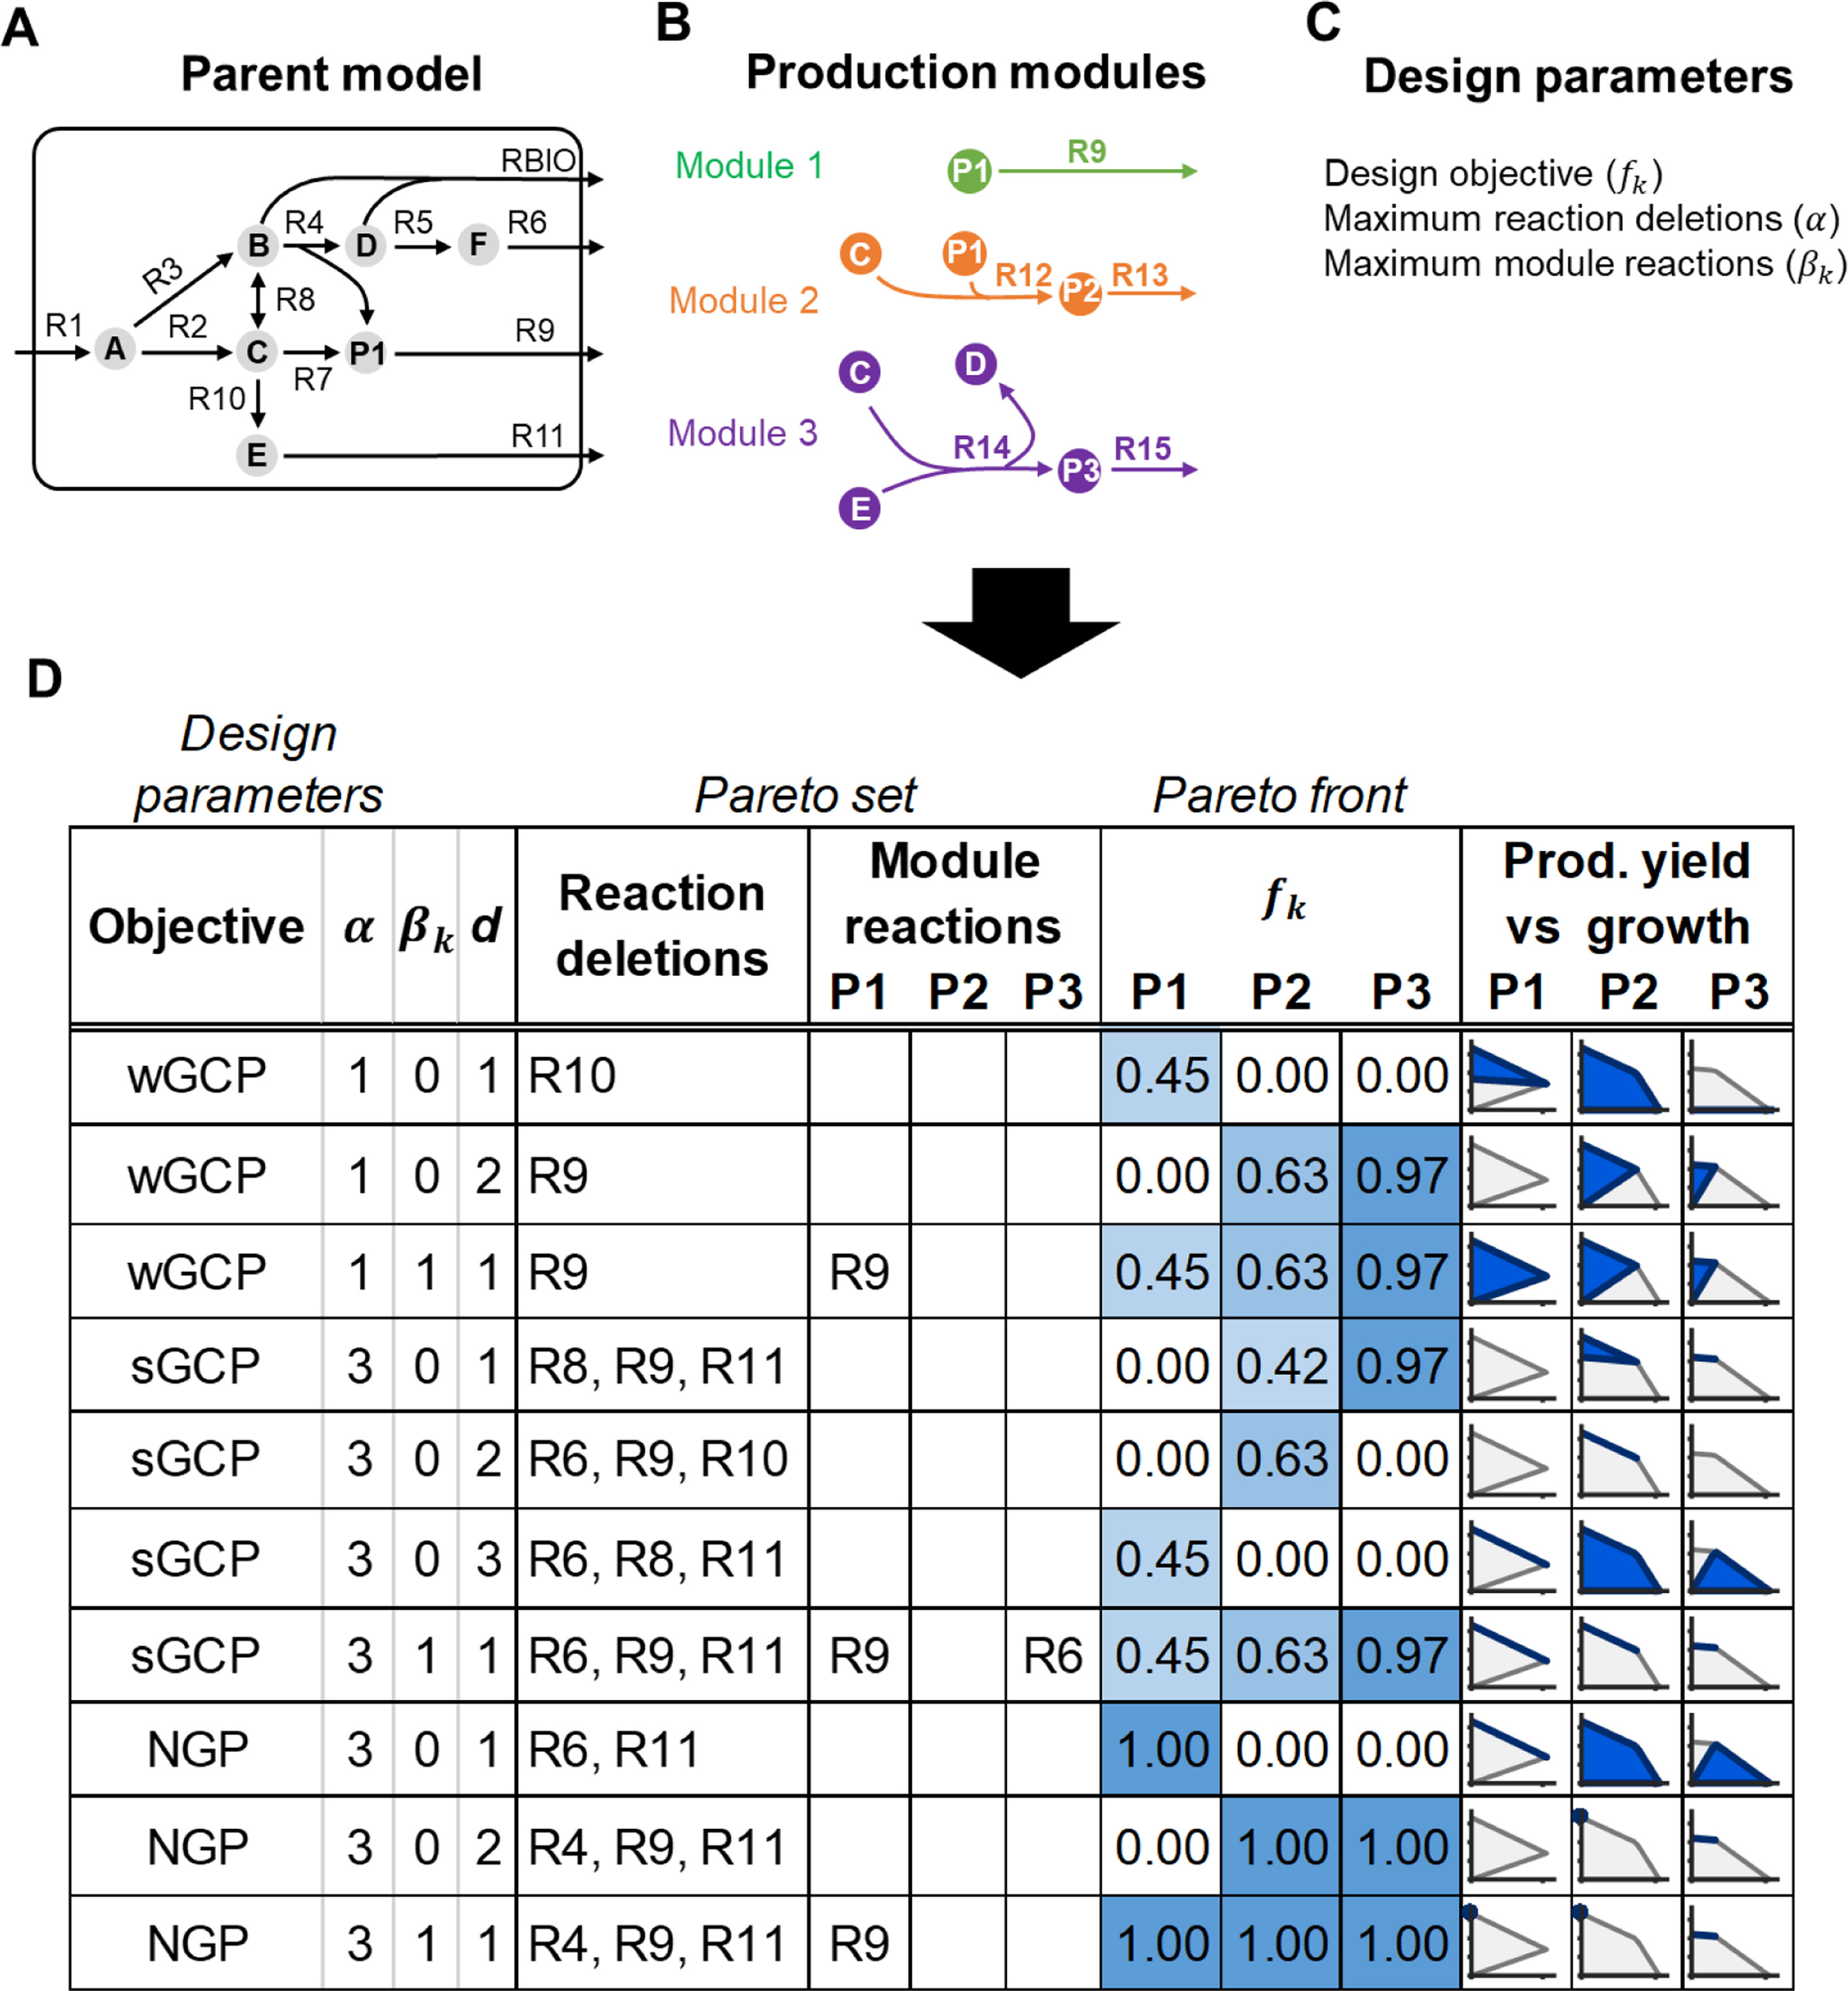
\includegraphics[width=\textwidth]{ms1-3}
    \caption[ModCell2 workflow and analysis]{
Illustration of ModCell2 workflow and analysis
including (\textbf{A}) parent model, (\textbf{B}) production modules,
(\textbf{C}) design parameters, and (\textbf{D}) simulation output for
Pareto set and Pareto front based on design input.
    }
    \label{fig:ms1-fig3}
\end{figure}
%}

Using various \(\alpha\)~and \(\beta_{k}\) values, ModCell2 simulation generated three \emph{wGCP}-\(\alpha\)\emph{-}\(\beta_{k}\)-\(d\), four \emph{sGCP}-\(\alpha\)\emph{-}\(\beta_{k}\)-\(d\) designs, and three \emph{NGP}-\(\alpha\)\emph{-}\(\beta_{k}\)-\(d\) designs, where \(d\) is the design solution index (Figure~\ref{fig:ms1-fig3}D).
For instance, by setting \(\alpha\)~= 3 and \(\beta_{k}\) = 0, we found three \emph{sGCP} designs including \emph{sGCP-3-0-1}, \emph{sGCP-3-0-2}, and \emph{sGCP-3-0-3}.
The first design \emph{sGCP-3-0-1} has a compatibility of 2 with the design objective values of 0.42 and 0.97 for the products P2 and P3, respectively.
In contrast, the \emph{sGCP-3-0-2} and \emph{sGCP-3-0-3} designs have compatibilities of only 1 with the design objectives of 0.63 for P2 and 0.45 for P1, respectively.

Based on all designs, we can clearly see the trade-offs for optimization of different products for \(\beta_{k}\) = 0.
However, setting \(\beta_{k} \geq 1\) helps increase the compatibility of a modular cell with different production modules.
In addition, we found that the Pareto front collapses into a utopia point as seen in the \emph{wGCP-1-1-1}, \emph{sGCP-3-1-1}, and \emph{NGP-3-1-1} designs.
For instance, the modular cell, \emph{sGCP-3-1-1}, is compatible with all three products.
The three corresponding optimal production strains can couple growth and product formation during the growth phase.
During the stationary phase, these strains produce the products at maximum theoretical yields.
In theory, a universal modular cell always exists, provided that enough reaction deletions and module reactions are used.
It might be more tractable to construct such a modular cell from a synthetic minimal cell using the bottom-up approach.
However, construction of a universal modular cell from a host organism (e.g., \emph{E.
coli}, \emph{S. cerevisiae}) using the top-down approach will require a significantly large number of genetic modifications, that might be challenging.


\subsection{Comparing ModCell2 designs with first-generation MODCELL and single product designs}

\subsubsection{ModCell2 can generate more and better designs than the
first-generation modular cell design platform}
To evaluate the algorithms and performance of ModCell2, we directly compared it with
MODCELL \citep{trinh2015} in two case studies, using the same
core model of \emph{E. coli} for production of five alcohols (ethanol,
propanol, isopropanol, butanol, and isobutanol) and 5 derived butyrate
esters (ethyl butyrate, propyl butyrate, isopropyl butyrate, butyl
butyrate, and isobutyl butyrate) from glucose (Figure~\ref{fig:ms1-fig4}A).

%\afterpage{%
\begin{figure}[p]
  \centering
  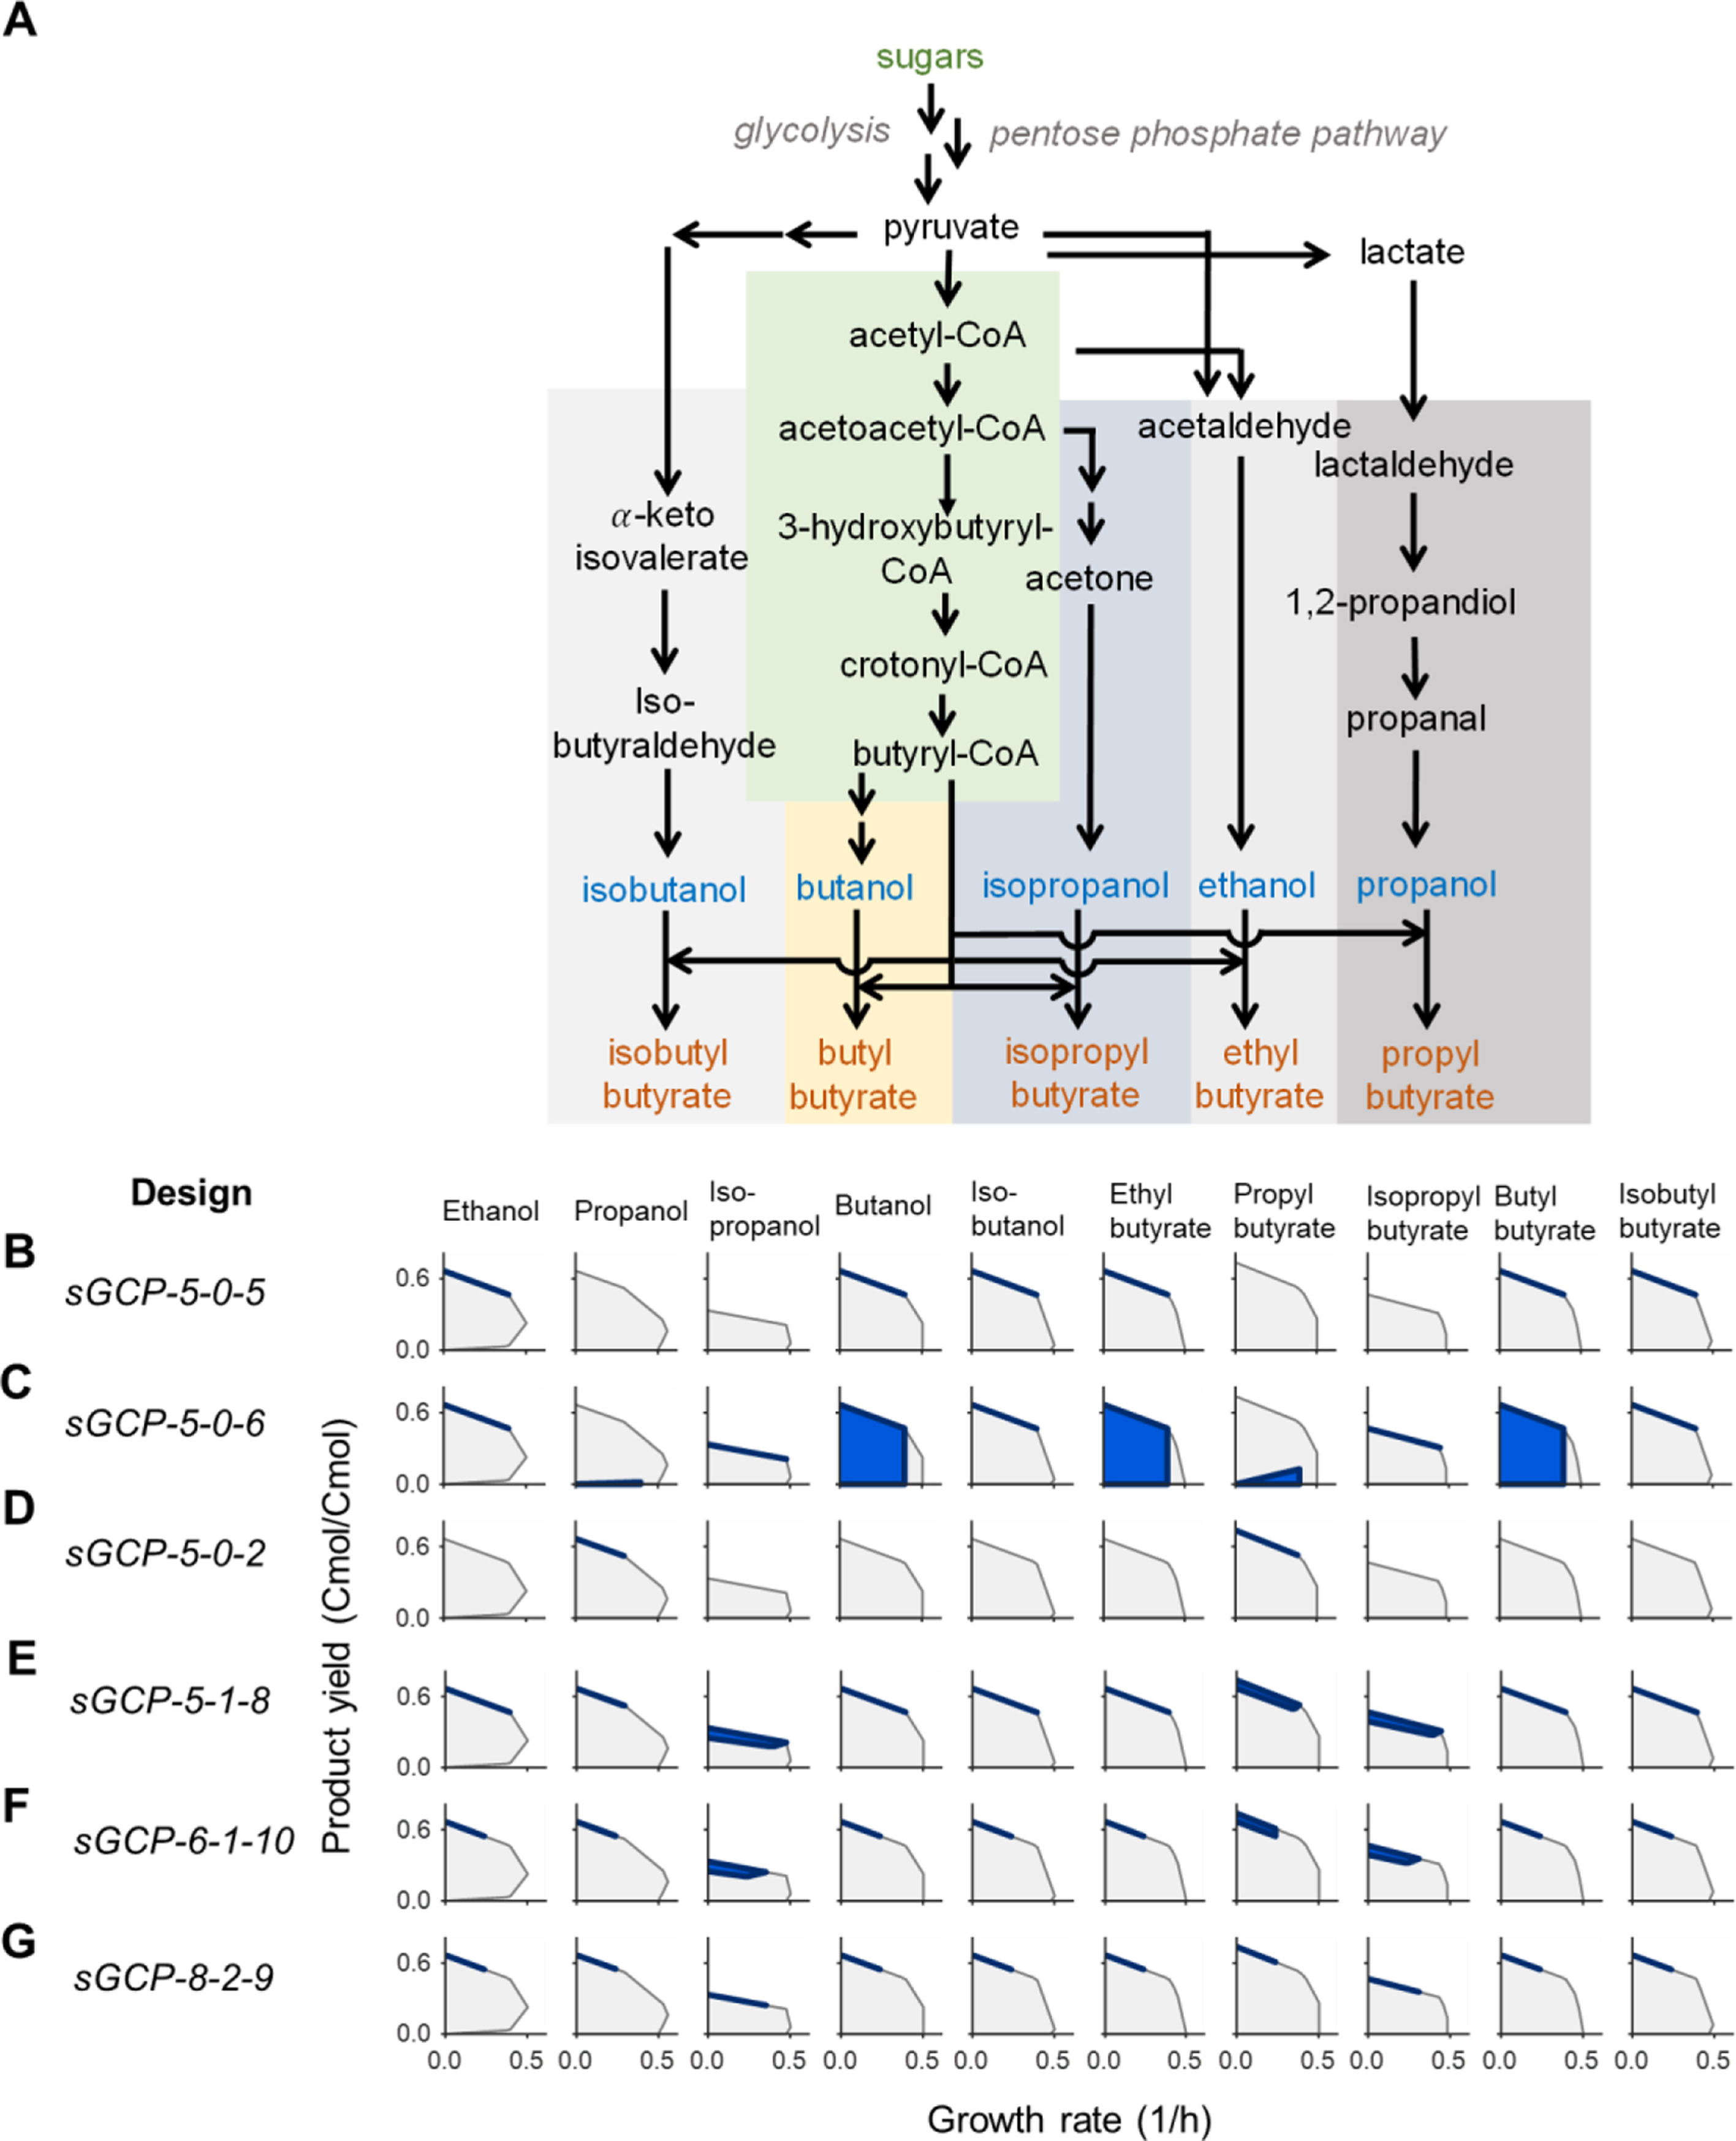
\includegraphics[width=\textwidth]{ms1-4}
    \caption[2-D metabolic phenotypic spaces of different \emph{sGCP} designs using the core metabolic model]{
The 2-D metabolic phenotypic spaces of different
\emph{sGCP} designs using the core metabolic model. (\textbf{A})
Metabolic map, \textbf{(B)} \emph{sGCP-5-0-5} design, \textbf{(C)}
\emph{sGCP-5-0-6} design, \textbf{(D)} \emph{sGCP-5-0-2} design,
\textbf{(E)} \emph{sGCP-5-1-8} design, \textbf{(F)} \emph{sGCP-6-1-10}
design, and \textbf{(G)} \emph{sGCP-8-2-9} design. For each panel, the
gray and blue areas correspond to the phenotypic spaces of the wildtype
and the optimal production strain, respectively.
    }
    \label{fig:ms1-fig4}
\end{figure}
%}

In the first case study, we fixed the reaction module, i.e.
\(\beta_{k} = 2\) for ethanol dehydrogenase (FEM5) and ethanol export reaction (TRA1), in ModCell2 to emulate the same input as MODCELL (Supplementary File S3).
The results showed that ModCell2 generated all the designs with the same \emph{sGCP} objective values like MODCELL (Figure~\ref{fig:ms1-fig4}B, 4C, 4D) together with other alternative solutions (Supplementary File S3).
Interestingly, ModCell2 only required 5 and 6 reaction deletions as opposed to 7 and 7 for the \emph{sGCP-5-0-5} and \emph{sGCP-5-0-6} designs, respectively.
By setting the maximum reaction deletions to \(\alpha \geq 6\), ModCell2 could find better design solutions with fewer deletion reaction requirement and higher objective values (Supplementary File S3).

In the second case study, we used the same model configuration but did not enforce the module reactions.
By setting \(\alpha = 5\) and \(\beta_{k} = 1\), we found the \emph{sGCP-5-1-8} design that is compatible with all products and achieves the same objective values for products found in \emph{sGCP-5-0-5}, \emph{sGCP-5-0-6}, and \emph{sGCP-5-0-2} (Figure~\ref{fig:ms1-fig4}E).
The desirable phenotypic spaces can be further constrained for many products if \(\alpha\) is increased from 5 to 6 (Figure~\ref{fig:ms1-fig4}F).
Remarkably, by setting \(\alpha = 8\) and \(\beta_{k} = 2\), we found a utopia point design, \emph{sGCP-8-2-9}, without any trade-off among design objectives (Figure~\ref{fig:ms1-fig4}G).
This utopia point design could not be achieved with \(\alpha <\) 8 regardless\(\ \)of any \(\beta_{k}\) value.

Overall, the results demonstrate that ModCell2 can efficiently compute the Pareto front of modular cell designs.
It can find better designs with fewer reaction deletion and module reaction requirements, improve design objective values, and enhance compatibility.

\subsubsection{ModCell2 can identify designs with more compatibility than
the conventional single-product designs}
To evaluate if the
conventional, single-product design strategy is suitable for modular
cell engineering, we first used OptKnock to generate \emph{wGCP} designs
for the same 10 target molecules independently with various allowable
reaction deletions (\(\alpha = 2,\ 3,\ \ldots,\ 7\)). Likewise, we
employed ModCell2 to produce \emph{wGCP} designs using the same
\(\alpha\) and various \(\beta\). To directly compare OptKnock and
ModCell2 solutions, we calculated the \emph{wGCP} design objective
values for all products based on each OptKnock solution (Supplementary
File S3). As expected, our result showed that ModCell2 and OptKnock
designs have the same highest objective values for each product (Figure
5A). However, several OptKnock solutions were always dominated by
ModCell2 solutions in all parameter configurations (Figure~\ref{fig:ms1-fig5}B). With
\(\alpha \geq 4\), ModCell2 could identify
\emph{wGCP-}\(\alpha\)\emph{-1} designs with the maximum compatibility
of 10, while the best OptKnock designs only achieved the highest
compatibility of 5 (Figure~\ref{fig:ms1-fig5}C, 5D).

Overall, ModCell2 can generate modular cells compatible with the maximum number of modules and achieve high objective values.
Single-product designs might not be compatible with a large number of products, and the solutions might be far from Pareto optimality.

%\afterpage{%
\begin{figure}[hbp]
  \centering
  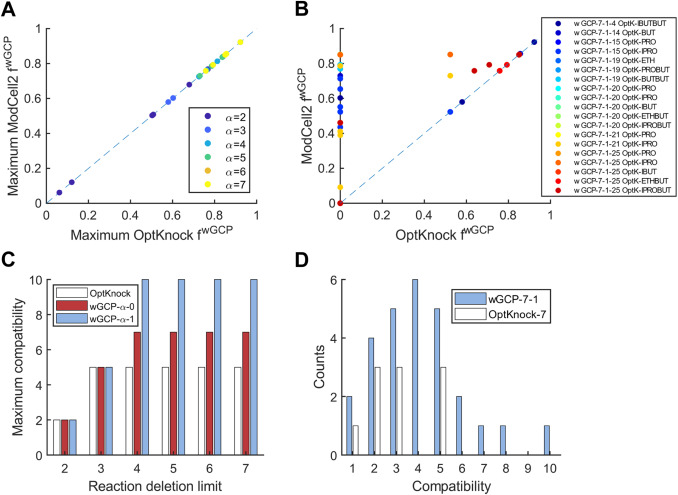
\includegraphics[width=\textwidth]{ms1-5}
    \caption[Comparison of strain design by OptKnock and Modcell2]{
Comparison of strain design by OptKnock and Modcell2.
(\textbf{A}) A correlation between the maximum objective values for each
product generated by OptKnock and the equivalent values attained by
ModCell2. Each point is colored based on the number of reaction
deletions, with warmer colors corresponding to more reaction deletions.
(\textbf{B}) A comparison between the Optknock objective vectors with at
most 7 reaction deletions and the representative ModCell2 objective
vector, \emph{wGCP-7-1} which dominates them. Each color circle
represents a pair of dominating \emph{wGCP} design and dominated
OptKnock solution (Supplementary File S3). (\textbf{C}) Maximum
compatibility of OptKnock designs (blue), \emph{wGCP} designs
    ($\beta_k=0$, orange), wGCP designs ($\beta_k = 1$,
yellow). (\textbf{D}) Compatibility distribution of Optknock ($\alpha = 7$,
orange) and \emph{wGCP-7-1} (blue).
    }
    \label{fig:ms1-fig5}
\end{figure}
%}

\subsection{Exploring emergent features of modular cell design using an \textit{E. coli} genome-scale network}

\subsubsection{Modcell2 can design modular cells using a large-scale
metabolic network.}
To demonstrate that ModCell2 can be applied for a
genome scale metabolic network, we tested it to generate \emph{wGCP}
designs for 20 target molecules with \(\alpha = 4\) and various
\(\beta_{k}\) (Supplementary File S4). The \(\alpha\) value was chosen
because with 4 deletions, OptKnock could identify single product designs
with objectives above 60\% of the theoretical maximum (Supplementary
File S5). With \(\beta_{k} = 0\), ModCell2 could identify modular cell
designs with compatibility of 17, for example, the \emph{wGCP-4-0-50}
design featuring deletion of ACALD (acetaldehyde dehydrogenase,
\emph{adhE}), ACKr/PTAr (acetate kinase, \emph{ack;}
phosphotransacetylase, \emph{pta}), GLYAT (glycine C-acetyltransferase,
\emph{kbl}), and LDH\_D (lactate dehydrogenase, \emph{ldhA}) (Figure~\ref{fig:ms1-fig6}A,
6D, Supplementary File S4). By analyzing all
\emph{wGCP-4-}\(\beta_{k}\)\emph{-}\(d\) designs (257 total for
\(\beta_{k}\) = 0, 1, 2, and 3), we found that the ethanol and D-lactate
production modules are most compatible with all modular cell designs
(Figure~\ref{fig:ms1-fig6}A, 6C, Supplementary File S4). Among reaction deletions,
\emph{LdhA} (86\% of designs), \emph{Pta} (38\%), and \emph{AdhE} (25\%)
are the most frequent deletion reactions (Figure~\ref{fig:ms1-fig6}B). This finding is
consistent with a comprehensive survey of metabolic engineering
publications \citep{winkler2015} showing that these deleted
reactions appeared in most of \emph{E. coli} engineered strains for
production of fuels and chemicals. The result supports the potential use
of modular cell engineering to systematically build modular platform
strains.

%\afterpage{%
\begin{figure}[!bp]
  \centering
  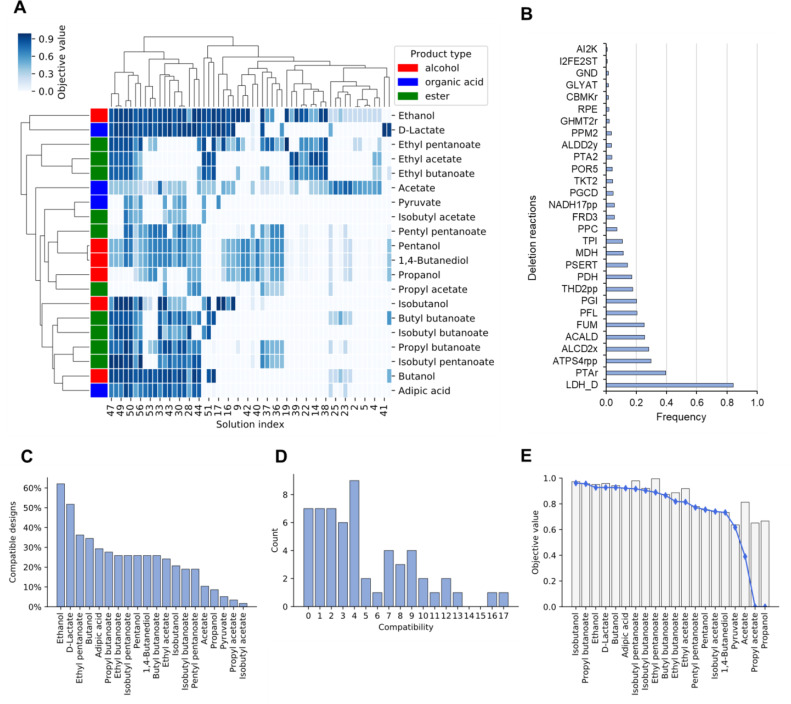
\includegraphics[width=\textwidth]{ms1-6}
    \caption[Analysis of \emph{wGCP} designs with genome-scale model]{
 Analysis of \emph{wGCP} designs with genome-scale model. \textbf{(A)} Pareto front of \emph{wGCP-4-0-d}. The
columns correspond to different designs labeled by their design index,
\emph{d}, where the rows correspond to different products. \textbf{(B)}
Frequency of the top deletion reactions. \textbf{(C)} Product
    compatibility distribution across designs. \textbf{(D)} Design
compatibility. \textbf{(E)} Tradeoff between modularity and performance.
The bars correspond to the maximum objective values attainable for each
product whereas the blue line represent the objective values of the
\emph{wGCP-4-0-48alternative} design.
    }
    \label{fig:ms1-fig6}
\end{figure}
%}

\subsubsection{ModCell2 designs can capture combinatorial characteristics
of production modules.} To evaluate whether ModCell2 could capture the
combinatorial properties among production modules, we analyzed the
Pareto front of \emph{wGCP-4-0-d} that have a total of 58 designs.
Hierarchical clustering of this Pareto front revealed certain products
with similar objective values across solutions, such as ethyl esters and
butyrate esters (Figure~\ref{fig:ms1-fig6}A). These products together were compatible
with different modular cells and exhibited metabolic similarity in their
production modules. Thus, ModCell2 could generate designs that capture
the combinatorial properties useful for modular cell engineering.

\subsubsection{ModCell2 can identify highly compatible modular cells}
Analysis of compatibility shows that certain modular cells can couple
with production modules that may not exhibit the combinatorial
properties (Figure~\ref{fig:ms1-fig6}D). However, there exists a tradeoff between the
number of feasible designs and degree of compatibility. Some modular
cell designs are compatible with up to 17 out of 20 products, for
instance, the most compatible design, \emph{wGCP-4-0-48}, featuring
deletions of ACALD (\emph{adhE}), ACKr/PTAr (\emph{ack}, \emph{pta}),
GND (phosphogluconate dehydrogenase, \emph{gnd}) and LDH\_D
(\emph{ldhA}) (Supplementary File S4). An alternative design
\emph{wGCP-4-0-48-alternative} also exists where deletion of G6PDH2r
(gluose-6-phosphate dehydrogenase, \emph{zwf}) is replaced by that of
GND, the first step in the oxidative pentose phosphate pathway. The gene
deletions in the design \emph{wGCP-4-0-48-alternative} are a subset of
the modular \emph{E. coli} strain TCS095, whose modular properties have
recently been validated experimentally \citep{wilbanks2017}.

To determine if modular cell design is a viable alternative to single-product design, we also analyzed a potential tradeoff between design performance and modularity by comparing the maximum value of each objective across all solutions in the Pareto front and the single-product design optima.
If production modules exhibit competing phenotypes, a modular cell will not achieve the same performance in all modules as a single-product design strain.
Analysis of the most compatible design \emph{wGCP-4-0-48-alternative} showed that it could achieve objectives within 4\% of the single-product optima in 14 products and within 10\% in 3 products (Figure~\ref{fig:ms1-fig6}E).
This result indicates that it is feasible to identify highly compatible modular cell designs without a significant tradeoff between performance and modularity.

\subsubsection{Analysis of potential tradeoff between robustness and
modularity can identify conserved metabolic features}
To evaluate the
robustness of modular cells, we analyzed the compatibility change
(\emph{CD}) of \emph{wGCP-4-0} designs with compatibilities of 4 or
greater (Figure S3 in Supplementary File 2). Remarkably, the result
shows that only 7.5\% of potential reaction deletions were detrimental
to the robustness of modular cells while the large remaining portion did
not affect \emph{CD} values. Out of the 85 reactions whose deletion
affected compatibility, only a few appeared consistently across the
designs. For instance, deletion of TPI (triose-phosphate isomerase,
\emph{tpi}) led to an average compatibility loss of 95\%, inactivating
most modular cell designs. Based on flux variability analysis, TPI must
operate in the forward direction by converting glycerone phosphate
(dhap) to glyceraldehyde-3-phosphate (g3p) to drive sufficient flux
through glycolysis and hence preventing synthesis of undesired
byproducts (D-lactate or 1,2-propanediol) from dhap. Likewise, deletion
of carbon dioxide and water transport and exchange reactions caused
compatibility loss across all designs. Pyruvate carboxylase (PPC) is an
important reaction to channel carbon flux through the Krebs cycle
\citep{coomes1985}, and hence, deletion of PPC reduces
compatibility in most modular cell designs with an average \emph{CL} of
43\%.

While some reaction deletions are critical for modular cell robustness, others are associated with specific products.
For example, deletion of PDH (pyruvate dehydrogenase complex, \emph{lpd/aceEF}) removes compatibility in all butanol-derived designs, indicating PFL (pyruvate formate lyase, \emph{pfl}) is not an appropriate route.
To make heterologous butanol-derived molecules under anaerobic conditions, FDH (NADH-dependent formate dehydrogenase, \emph{fdh}) is required in butanol-derived modules where enzymatic reaction pairs of PFL and FDH could substitute PDH known to be anaerobically inhibited.

Overall, analysis of tradeoff between modularity and robustness can identify not only the conserved metabolic features of modular cells but also potential bottlenecks in specific production modules.

\subsubsection{Enabling metabolic switch among different design
objectives using ModCell2}

The ability to dynamically control growth and production phases can potentially enhance product titers, rates, and yields.
For instance, two-phase fermentation can be employed where growth phase is optimized for biomass synthesis and stationary phase for chemical production \citep{klamt2018}.
Using ModCell2, we investigated the feasibility to design optimal strains to toggle switch desirable production phenotypes\emph{.}
To design a \emph{wGCP}$\rightarrow$\emph{NPG} metabolic switch, we first used our reference \emph{wGCP} design as a parent strain (Figure~\ref{fig:ms1-fig7}A) and then employed ModCell2 to identify the most compatible \emph{wGCP}$\rightarrow$\emph{NPG} designs.
With 5 additional deletions, we could find \emph{wGCP}$\rightarrow$NPG designs that encompass both \emph{wGCP} and \emph{NPG} phenotypes, for instance, the \emph{sup-NGP-5-0-23} design featuring deletion of PGI (glucose-6-phosphate isomerase, \emph{pgi}), MDH (malate dehydrogenase, \emph{mdh}), ASPT (L-aspartase, \emph{aspT}), Tkt2 (transketolase, \emph{tktB}), and ATPS4rpp (ATP synthase, \emph{atp}) (Figure~\ref{fig:ms1-fig7}B).
The deletion reactions in the \emph{wGCP}$\rightarrow$NPG designs appear in both catabolic (PGI, ATPS4tpp) and anabolic (ASP, TKT2) processes, responsible for growth disruption and direction of carbon flow to the biosynthesis of target products.

Likewise, we used ModCell2 to design a \emph{wGCP}$\rightarrow$\emph{sGCP} metabolic switch\emph{.} We identified the most compatible \emph{wGCP}$\rightarrow$\emph{sGCP} designs with 6 additional deletions, for instance, the \emph{sup-sGCP-6-0-39} design featuring the deletion of MGSA (Methylglyoxal synthase, \emph{mgsA}), ALCD2x (alcohol dehydrogenase, \emph{adhE}), PFL, MDH, FADRx (FAD reductase, \emph{fadI}), and GLUDy (NADP\textsuperscript{+}dependent glutamate dehydrogenase, \emph{gdhA}) (Figure~\ref{fig:ms1-fig7}C).
Different from the \emph{wGCP}$\rightarrow$\emph{NGP} metabolic switch, all deletions in the \emph{wGCP}$\rightarrow$\emph{sGCP} designs are involved the elimination of biosynthesis pathways of undesirable byproducts.

While it is feasible to metabolically switch among different production phenotypes, it not only requires more reaction deletions but also reduces the product compatibility.
For instance, the \emph{wGCP}$\rightarrow$sGCP and \emph{wGCP}$\rightarrow$NGP designs are only compatible with 5 products while the \emph{wGCP} parent design have a compatibility of 17 out of 20 products with 4 deletions.
The main reason is that both \emph{wGCP}$\rightarrow$\emph{sGCP} and \emph{wGCP}$\rightarrow$\emph{NGP} designs must eliminate all possible redundant pathways that result in biosynthesis of undesirable byproducts.


\section{Conclusion}

In this study, we developed a multi-objective strain design platform for modular cell engineering.
With a new developed algorithm and computational platform, ModCell2 enables flexible design of modular cells that can couple with production modules to exhibit desirable production phenotypes.
In comparison to the first-generation strain design platform, ModCell2 can handle large-scale metabolic networks and identify better solutions that require fewer genetic modifications and exhibit more product compatibility.
Different from the conventional single-product strain design, ModCell2 can find solutions that are Pareto optimal with negligible tradeoffs among modularity, performance, and robustness.
We envision ModCell2 is a useful tool to implement modular cell engineering and fundamentally study modular designs in natural and synthetic biological systems.

%\afterpage{%
\begin{figure}[p]
  \centering
  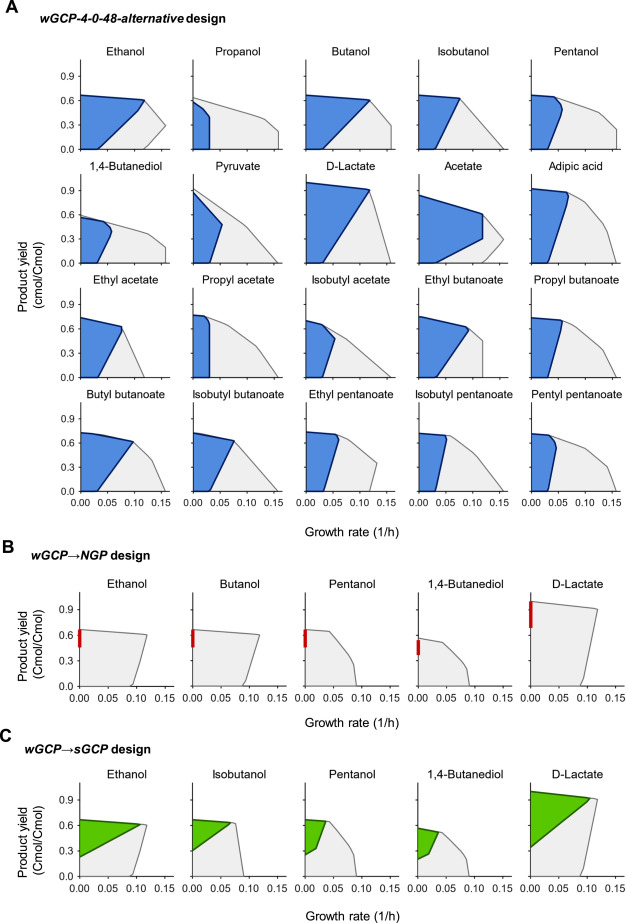
\includegraphics[height=.86\textheight]{ms1-7}
    \caption[Production phenotypes of proposed designs]{
Production phenotypes of (\textbf{A}) the wild type
(gray) and the representative, highly-compatible design
\emph{wGCP-4-0-48-alternative} (blue), (\textbf{B}) the
\emph{wGCP}$\rightarrow$\emph{NPG} design, \emph{sup-NGP-5-0-23}, and (\textbf{C})
the \emph{wGCP}$\rightarrow$\emph{sGCP} design, \emph{sup-sGCP-6-0-39}.
    }
    \label{fig:ms1-fig7}
\end{figure}
%}

%\textbf{ACKNOWLEDGEMENTS}
%
%This research was financially supported in part by the NSF CAREER Award (NSF\#1553250) and the DOE subcontract Grant (DE-AC05-000R22725) by the Center of Bioenergy Innovation (CBI), the U.S.
%Department of Energy Bioenergy Research Center funded by the Office of Biological and Environmental Research in the DOE Office of Science.
%The funders had no role in the study design, data collection and analysis, decision to publish, or preparation of the manuscript.
%



    \chapter{Comparison of multi-objective evolutionary algorithms to solve the modular cell design problem} %\label{ch:conclusion}

\newcommand\HV{\mathit{HV}}
\newcommand\GD{\mathit{GD}}
\newcommand\IGD{\mathit{IGD}}

\disclose{garcia2019c}
Supplementary Material 1 is provided as an attachement.

%{{{ abstract (max ~200 words)

\section*{Abstract}
A large space of chemicals with broad industrial and consumer applications could be synthesized by engineered microbial biocatalysts. However, the current strain optimization process is prohibitively laborious and costly to produce one target chemical and often requires new engineering efforts to produce new molecules. To tackle this challenge, modular cell design based on a chassis strain that can be combined with different product synthesis pathway modules has been recently proposed.
This approach seeks to minimize unexpected failure and avoid task repetition, leading to a more robust and faster strain engineering process. In our previous study, we mathematically formulated
the modular cell design problem based on the multi-objective optimization framework. In this study, we evaluated a library of state-of-the-art multi-objective evolutionary algorithms (MOEAs) to identify the most effective method to solve the modular cell design problem.
Using the best MOEA, we found better solutions for modular cells compatible with many product synthesis modules. Furthermore, the best performing algorithm could provide better and more diverse design options that might help increase the likelihood of successful experimental implementation.
We identified key parameter configurations to overcome the difficulty associated with multi-objective optimization problems with many competing design objectives.
Interestingly, we found that MOEA performance with a real application problem, e.g., the modular strain design problem, does not always correlate with artificial benchmarks. Overall, MOEAs provide powerful tools to solve the modular cell design problem for novel biocatalysis.
%}}}
\section{Introduction}
Multi-objective optimization is a powerful mathematical toolbox widely used in engineering disciplines to solve problems with multiple conflicting design objectives \cite{coello2004}.
For example, in the field of chemical engineering, multi-objective optimization has been applied to balance design conflicts in the performance, material and energy requirements, and environmental sustainability of many different chemical processes \cite{rangaiah2009}. In industrial biotechnology, with recent advancements in synthetic biology and metabolic engineering, microorganisms can be genetically modified to produce a large space of molecules with broad applications using renewable lignocellulosic biomass or waste products as feedstocks \cite{trinh2016, lee2019}.
However, the current strain design process is prohibitively laborious and expensive for broad industrial application \cite{nielsen2016}. To overcome this challenge, recent studies have proposed the application of modular design principles commonly used in engineering \cite{bonvoisin2016} to microbial biocatalysis \cite{trinh2012, trinh2015, garcia2019, garcia2019b}.
This modular cell design approach, known as ModCell, uses multi-objective optimization to account for the competing cellular objectives when cellular metabolism is (re)designed in a modular fashion to produce a diverse class of target chemicals. ModCell has been experimentally demonstrated for biosynthesis of alcohols \cite{trinh2011, trinh2012, wilbanks2017} and esters \cite{layton2014, layton2016, layton2016b, wierzbicki2016, lee2018} in \textit{Escherichia coli}.

Despite the broad applicability of multi-objective optimization problems (MOPs) in engineering design, powerful solution algorithms remain elusive. Two approaches can be used to solve MOPs, including multi-objective evolutionary algorithms (MOEAs) and mixed integer linear programming (MILP) algorithms.
Unlike MOEA, MILP can ensure that the identified MOP solutions are optimal.
Nonetheless, MOEAs are widely used due to the following advantages over MILP: (i) computational scalability for large-scale networks by implementing efficient parallelization algorithms \cite{coello2007}, (ii) compatibility with non-linear objectives and constraints, and (iii) unbiased sampling of Pareto optimal solutions without a need to pre-specify objective preference \cite{marler2004}.
MOEAs are based on a more general type of optimization method known as evolutionary algorithms, where candidate solutions, that represent individuals of a population, are iteratively modified using heuristic rules to increase their fitness (i.e., objective function values).
Recently, much attention has been placed in the development of MOEAs to solve many-objective problems (e.g., problems with 4 or more objectives) that often correspond to real-world applications, but can be very challenging to solve with conventional MOEAs \cite{li2015}.
For the case of ModCell problem, the popular MOEA NSGAII \cite{matlabdoc, deb2001} was used to design a modular cell under 20 different production modules \cite{garcia2019}.
Due to a large space of molecules that can potentially be synthesized by modular cells, scalability issues are expected to occur when constructing modular cells that are designed to be compatible with tenths or hundreds of products.
Furthermore, using the best solver algorithm(s) allows to explore a more diverse design space, resulting in better choices for experimental implementation.

Many MOEAs have been proposed over the past two decades since the inception of landmark algorithms such as NSGAII \cite{deb2002} and SPEA2 \cite{zitzler2001}.
New MOEAs are benchmarked against libraries of artificial problems with known solutions \cite{zitzler2000, deb2002b}, and are expected to show enhanced performance for a subset of these problems in terms of scalability, identification of Pareto optimal solutions, and number of simulation generations needed to converge.
This benchmarking methodology does not always reflect MOEA performance for general problems, since specialized parameter configurations or heuristics are often used and can lead to drastically different performance towards a specific problem of interest.
Thus, the best MOEA for a certain application problem needs to be determined empirically.
In this study, we evaluated a library of state-of-the-art MOEAs to solve the multi-objective ModCell problem, with the focus on many-objectives methods.
Several cases study of increasing difficulty were examined using common performance indicators of solution optimality and diversity, and critical algorithm parameters that determine solution quality were also investigated.

%%%%%%%%%%%%%%%%%%%%%%%%%%%%%%%%%%%%%%%%%%

\section{Methods}
\subsection{Multi-objective modular cell design}
Modular cell design enables rapid generation of optimal production strains with desirable phenotypes from a modular (chassis) cell \cite{garcia2019}, requiring mimimal strain optimization cycles. These production strains are assembled from a modular cell and various compatible pathway modules. A modular cell is constructed by eliminating genes from a parent strain to maintain only core metabolic pathways shared across all pathway modules. Each module enables an optimized target product synthesis phenotype that leads to high yields, titers, and production rates. The different biochemical nature of each target metabolite can make the objectives compete with each other, turning the modular cell design problem into a multi-objective optimization problem known as ModCell2 \cite{garcia2019}:

\begin{alignat}{3}
	& \underset{ \; y_j, z_{jk}}{\max} \quad (f_1, f_2, \ldots, f_{|\mathcal{K}|})^T \quad \text{s.t.}  \label{eq4:of1} \\
	&  \quad f_k \in \, \text{arg }\underset{}{\text{max}} \Bigg\{ \frac{1}{f_k^{max}}\sum_{j \in \mathcal{J}_k} c_{jk}  v_{jk} \quad \text{s.t.} \label{eq4:of2}\\
	& \quad \qquad \sum_{j\in \mathcal{J}_k}S_{ijk}v_{jk} = 0 && \text{for all } i \in \mathcal{I}_k  \label{eq4:mb}\\
	& \quad \qquad  l_{jk} \le v_{jk} \le u_{jk}  && \text{for all } j \in \mathcal{J}_k \label{eq4:rb}\\
	& \quad \qquad  l_{jk} d_{jk} \le v_{jk} \le u_{jk} d_{jk} && \text{for all } j \in \mathcal{C} \label{eq4:db}\\
	& \quad \qquad \mathrm{where} \; d_{jk} = y_j \lor z_{jk} \; \Bigg\} && \text{for all } k \in \mathcal{K} \nonumber \\
	& \quad z_{jk}\le (1-y_j) && \text{for all } j \in \mathcal{C}, \, k \in \mathcal{K} \label{eq4:mr1}\\
	& \quad \sum_{j \in \mathcal{C}}z_{jk} \le \beta_k && \text{for all } k \in \mathcal{K} \label{eq4:mr2} \\
	& \quad \sum_{j \in \mathcal{C}} (1-y_j) \le \alpha \label{eq4:a}
\end{alignat}

\noindent where $\mathcal{I}_k$, $\mathcal{J}_k$, and $\mathcal{K}$ are the sets of metabolites, reactions, and associated production metabolic networks (i.e., the combination of the chassis organism with a specific product synthesis pathway), respectively.
The optimization problem seeks to simultaneously maximize all objectives $f_k$ \eqref{eq4:of1}.
The desirable phenotype $f_k$ for production module $k$ is determined based on key metabolic fluxes $v_{jk}$ (mmol/gDCW/h) predicted by the constraint-based metabolic model (\ref{eq4:of2}-\ref{eq4:db}) \cite{palsson2015}.
For example, the weak growth coupled to product formation (\emph{wGCP}), a common design objective, requires a high minimum product synthesis rate at the maximum growth-rate, enabling growth selection of optimal production strains. Thus, in \emph{wGCP} design, the inner optimization problem seeks to maximize growth rate while calculating the minimum product synthesis rate through the linear objective function \eqref{eq4:of2} (where {$c_{jk}$ is $1$ and $-0.0001$ for $j$ corresponding to the biomass and product reactions across all networks $k$, respectively, and 0 otherwise)
subject to: (i) mass-balance constraints \eqref{eq4:mb}, where $S_{ijk}$ represents the stoichiometric coefficient of metabolite $i$ in reaction $j$ of production network $k$, (ii) flux bound constraints \eqref{eq4:rb} that determine reaction reversibility and available substrates, where $l_{jk}$ and $u_{jk}$ are lower and upper bounds respectively, and (iii) genetic manipulation constraints \eqref{eq4:db}, i.e., deletion of a reaction $j$ in the chassis through the binary indicator $y_{j}$, or insertion of a reaction $j$ in a specific production network $k$ through the binary indicator $z_{jk}$.
The maximum product synthesis rate of each production network $k$, $f_k^{max}$, is determined by maximizing the product synthesis reaction subject to (\ref{eq4:mb}-\ref{eq4:rb}), allowing to bound $f_k$ in \textit{wGCP} between 0 and 1.
Only a subset of all metabolic reactions, $\mathcal{C}$, are considered as candidates for deletion, since many of the reactions in the metabolic model cannot be manipulated to enhance the target phenotype.
Certain reactions can be deleted in the chassis but inserted back to specific production modules, enabling the chassis to be compatible with a broader number of modules \eqref{eq4:mr1}.
The numbers of module-reaction additions and reaction deletions in the chassis are constrained by the parameters $\beta_k$ \eqref{eq4:mr2} and $\alpha$ \eqref{eq4:a}, respectively, to avoid unnecessary genetic manipulations that are generally time-consuming to implement and can lead to unforeseen phenotypes.

\subsection{Optimal solutions for a multi-objective optimization problem}
Optimal solutions for a MOP (\ref{eq4:of1}-\ref{eq4:a}) are defined based on the concept of domination: A vector $a=(a_1,\dots,a_K)^T$ \textit{dominates} another vector $b=(b_1,\dots ,b_K)^T$, denoted as  $a\prec b$ if and only if $a_i\ge b_i \; \forall i\in\{1,2,\dots,K\}$ and $a_i\ne b_i$ for at least one $i$.
Letting $x$ be the design variables (i.e., $y_j$ and $z_{jk}$) and $X$ be the feasible set determined by the problem constraints (\ref{eq4:of2}-\ref{eq4:a}), a feasible solution $x^* \in X$ of the MOP is called a Pareto optimal solution if and only if  there does not exists a vector $x'\in X$ such that $F(x')\prec F(x^*)$.
The set of all Pareto optimal solutions is called Pareto set:
\begin{equation}
\mathit{PS}:=\{x \in X:\nexists \, x' \in X, F(x') \prec F(x)\}
\end{equation}
The projection of the Pareto set in the objective space is denoted as Pareto front:
\begin{equation}
\mathit{PF}:=\{F(x): x \in PS \}
\end{equation}


\subsection{MOEA selection}
To find the best MOEAs for ModCell2, we evaluated a recent and comprehensive set of MOEAs implemented in the PlatEMO platform \cite{tian2017}.
From over 50 algorithms available in PlatEMO, we selected 2 methods for benchmark study, including NSGAII/gamultiobj and MOEAIGDNS, and 8 methods that have been specifically developed to tackle many-objective problems with discrete variables like ModCell2, including ARMOEA, EFRRR, MaOEADDFC, SPEAR, tDEA, BiGE, NSGAIII, and SPEA2SDE (Table~\ref{tab4:moeas}).
It should be noted that gamultiobj is an alternative implementation of the NSGAII algorithm available in Matlab.


\begin{table}[H]
    \caption[Summary of MOEAs]{Summary of MOEAs used in this study}
\centering
%% \tablesize{} %% You can specify the fontsize here, e.g., \tablesize{\footnotesize}. If commented out \small will be used.
%Table: MOEA summary
\rowcolors{2}{gray!25}{white}
\begin{tabular}{cm{6.5cm}m{4cm}c}
	\toprule
	Abbreviation & Name & Notes & Reference \\
	\midrule
	NSGAII & Non-dominated sorting genetic algorithm 2 & Highly applied MOEA & \cite{deb2002} \\
	gamultiobj & Matlab implementation of NSGAII &  Used in the original ModCell2 study\cite{garcia2019} & \cite{matlabdoc} \\
	MOEAIGDNS & Multi-objective evolutionary algorihtm based on an enhanced inverted generational distance metric & General MOEA with an implementation that works well with discrete variables & \cite{tian2016b} \\

	ARMOEA	& Adapation to reference points multi-objective evolutionary algorithm  & Many-objective EA based on MOEAIGDNS 	& \cite{tian2018} \\
	EFRRR	& Ensemble fitness ranking with ranking restriction	& Many-objective EA	& \cite{yuan2016a} \\
		MaOEADDFC & Many-objective evolutionary algorithm based on directional diversity and favorable convergence	& Many-objective EA	& \cite{cheng2015} \\
	SPEAR	& Strength Pareto evolutionary algorithm based on reference direction	& Many-objective EA	& \cite{jiang2017} \\
	tDEA	& $\theta$-dominance evolutionary algorithm	& Many-objective EA	& \cite{yuan2016} \\
	BiGE	& Bi-goal evolution	& Many-objective EA	& \cite{li2015a} \\
	NSGAIII & Non-dominated sorting genetic algorithm 3 	& Many-objective EA	& \cite{deb2014} \\
	SPEA2SDE & Strength Pareto evolutionary algorithm 2 with shift-based density estimation	& Many-objective EA	& \cite{li2014} \\
 \hline
\end{tabular}




    \label{tab4:moeas}
\end{table}

\subsection{Performance metrics}
To evaluate the performance of different MOEAs for a given problem, each algorithm was ran for the same number of generations, and the resulting solutions, known as Pareto front approximations, are compared using functions that measure two qualities: (i)
solution accuracy, i.e., to determine how similar the solution is to the true Pareto front and (ii) solution diversity, i.e., to evaluate how well distributed are the points in the solution.
We selected the top 5 most used  metrics according to a recent literature survey \cite{riquelme2015}.
These include, in order of popularity, hypervolume ($\HV$), generational distance ($\GD$), epsilon indicator ($\epsilon$), inverted generational distance ($\IGD$), and coverage ($C$).
Based on a recent study \cite{schutze2012}, we considered the average Hausdorff distance ($\Delta_p$), that combines $\GD$ and $\IGD$, and hence simplified the number of performance metrics to 4 in our study. These metrics are defined as follows:


$\HV$: This metric measures the volume occupied by the union of the smallest hyperboxes formed by each point in the Pareto front approximation and the reference point.  This Pareto front approximation corresponds to the solution of a specific MOEA (denoted as $\PF$) and the reference point is selected to be greater or equal to the maximum value attainable by any objective, which in our case is $\vec{1}$ (Figure~\ref{fig4:example}a):
\begin{equation}
	\HV = \bigcup\limits_{i\in I}\mathrm{Volume}(\mathrm{Box}(\PF_i,\vec{1})) \label{eq4:hv}
\end{equation}
where $I$ is the index set of $\PF$ points.

$\GD$: This metric measures the distance between the solution $\PF$ and the best Pareto front approximation determined by combining non-dominated points from all MOEA solutions of a specific case study, denoted $\PF^*$. More specifically, $\GD$ corresponds to the average Euclidean distance between each point in $\PF$ and the nearest point in $\PFs$, denoted as $d_i=\min\limits_{k \in K}\left( \sum\limits_{j \in J}(\PF_{ij} -\PFs_{kj})^2 \right)^{\frac{1}{2}}$, where $I$ ($i \in I$), $K$ ($k \in K$), and $J$ ($j \in J$) correspond to the index sets of $\PF$ points, $\PFs$ points, and problem objectives, respectively (Figure~\ref{fig4:example}b):
\begin{equation}
	 \GD = \frac{\sum\limits_{i \in I} d_i}{|I|}
\end{equation}

$\IGD$: This metric measures the distance between $\PF$ and $\PF^*$. It is determined by the average Euclidean distance between each point in $\PFs$ and the nearest point in $\PF$ denoted $\hat{d}_k=\min\limits_{i \in I}\left( \sum\limits_{j \in J}(\PFs_{kj} - \PF_{ij})^2 \right)^{\frac{1}{2}}$ (Figure~\ref{fig4:example}b):
\begin{equation}
	\IGD = \frac{\sum\limits_{k \in K} \hat{d}_k}{|K|}
\end{equation}

$\Delta_p$: This metric combines $\mathit{GD}$ and $\mathit{IGD}$ metric and thus has superior properties \cite{schutze2012}:
\begin{equation}
	 \Delta_p = \max(\mathit{GD},\mathit{IGD})
\end{equation}

$C$: This metric determines the fraction of $\PFs$ captured by the solution $\PF$ (Figure~\ref{fig4:example}c):
\begin{equation}
	C = \frac{|\PF \cap \PFs|}{|\PFs|} = \frac{|\{ k \in K : \exists i \in I \textrm{ such that } \PFs_{kj} = \PF_{ij} \textrm{ for all } j \in J \}|}{|K|}
\end{equation}

$\epsilon$: This metric is the additive epsilon indicator \cite{zitzler2002} that measures the smallest value to be added to any point in $\PF$ to make it non-dominated with respect to some point in  $\PFs$. In other words, it is the smallest value $\epsilon$ such that for any solution in $\PFs$ there is at least one solution in $\PF$ that is not worse by a difference of $\epsilon$ (Figure~\ref{fig4:example}d):
\begin{equation}
	\epsilon = \inf\{\epsilon \in \mathbb{R} : \textrm{for all }i \in I \, \exists k \in K \textrm{ such that } \PF_{ij} + \epsilon \ge \PFs_{kj} \textrm{ for all } j \in J\}
\end{equation}

Use of these metrics can be illustrated with a two-objective design example with 4 generations of improving Pareto front approximations, where the final Pareto front is used as a reference (i.e., $\PFs$) (Figure~\ref{fig4:example}e). As the Pareto fronts contain points that dominate the previous generations, all metrics decrease monotonically with the exception of $C$ that increases to a value of 1 when both Pareto front approximation and reference are the same (Figure~\ref{fig4:example}f).

\begin{figure}[H]
\centering
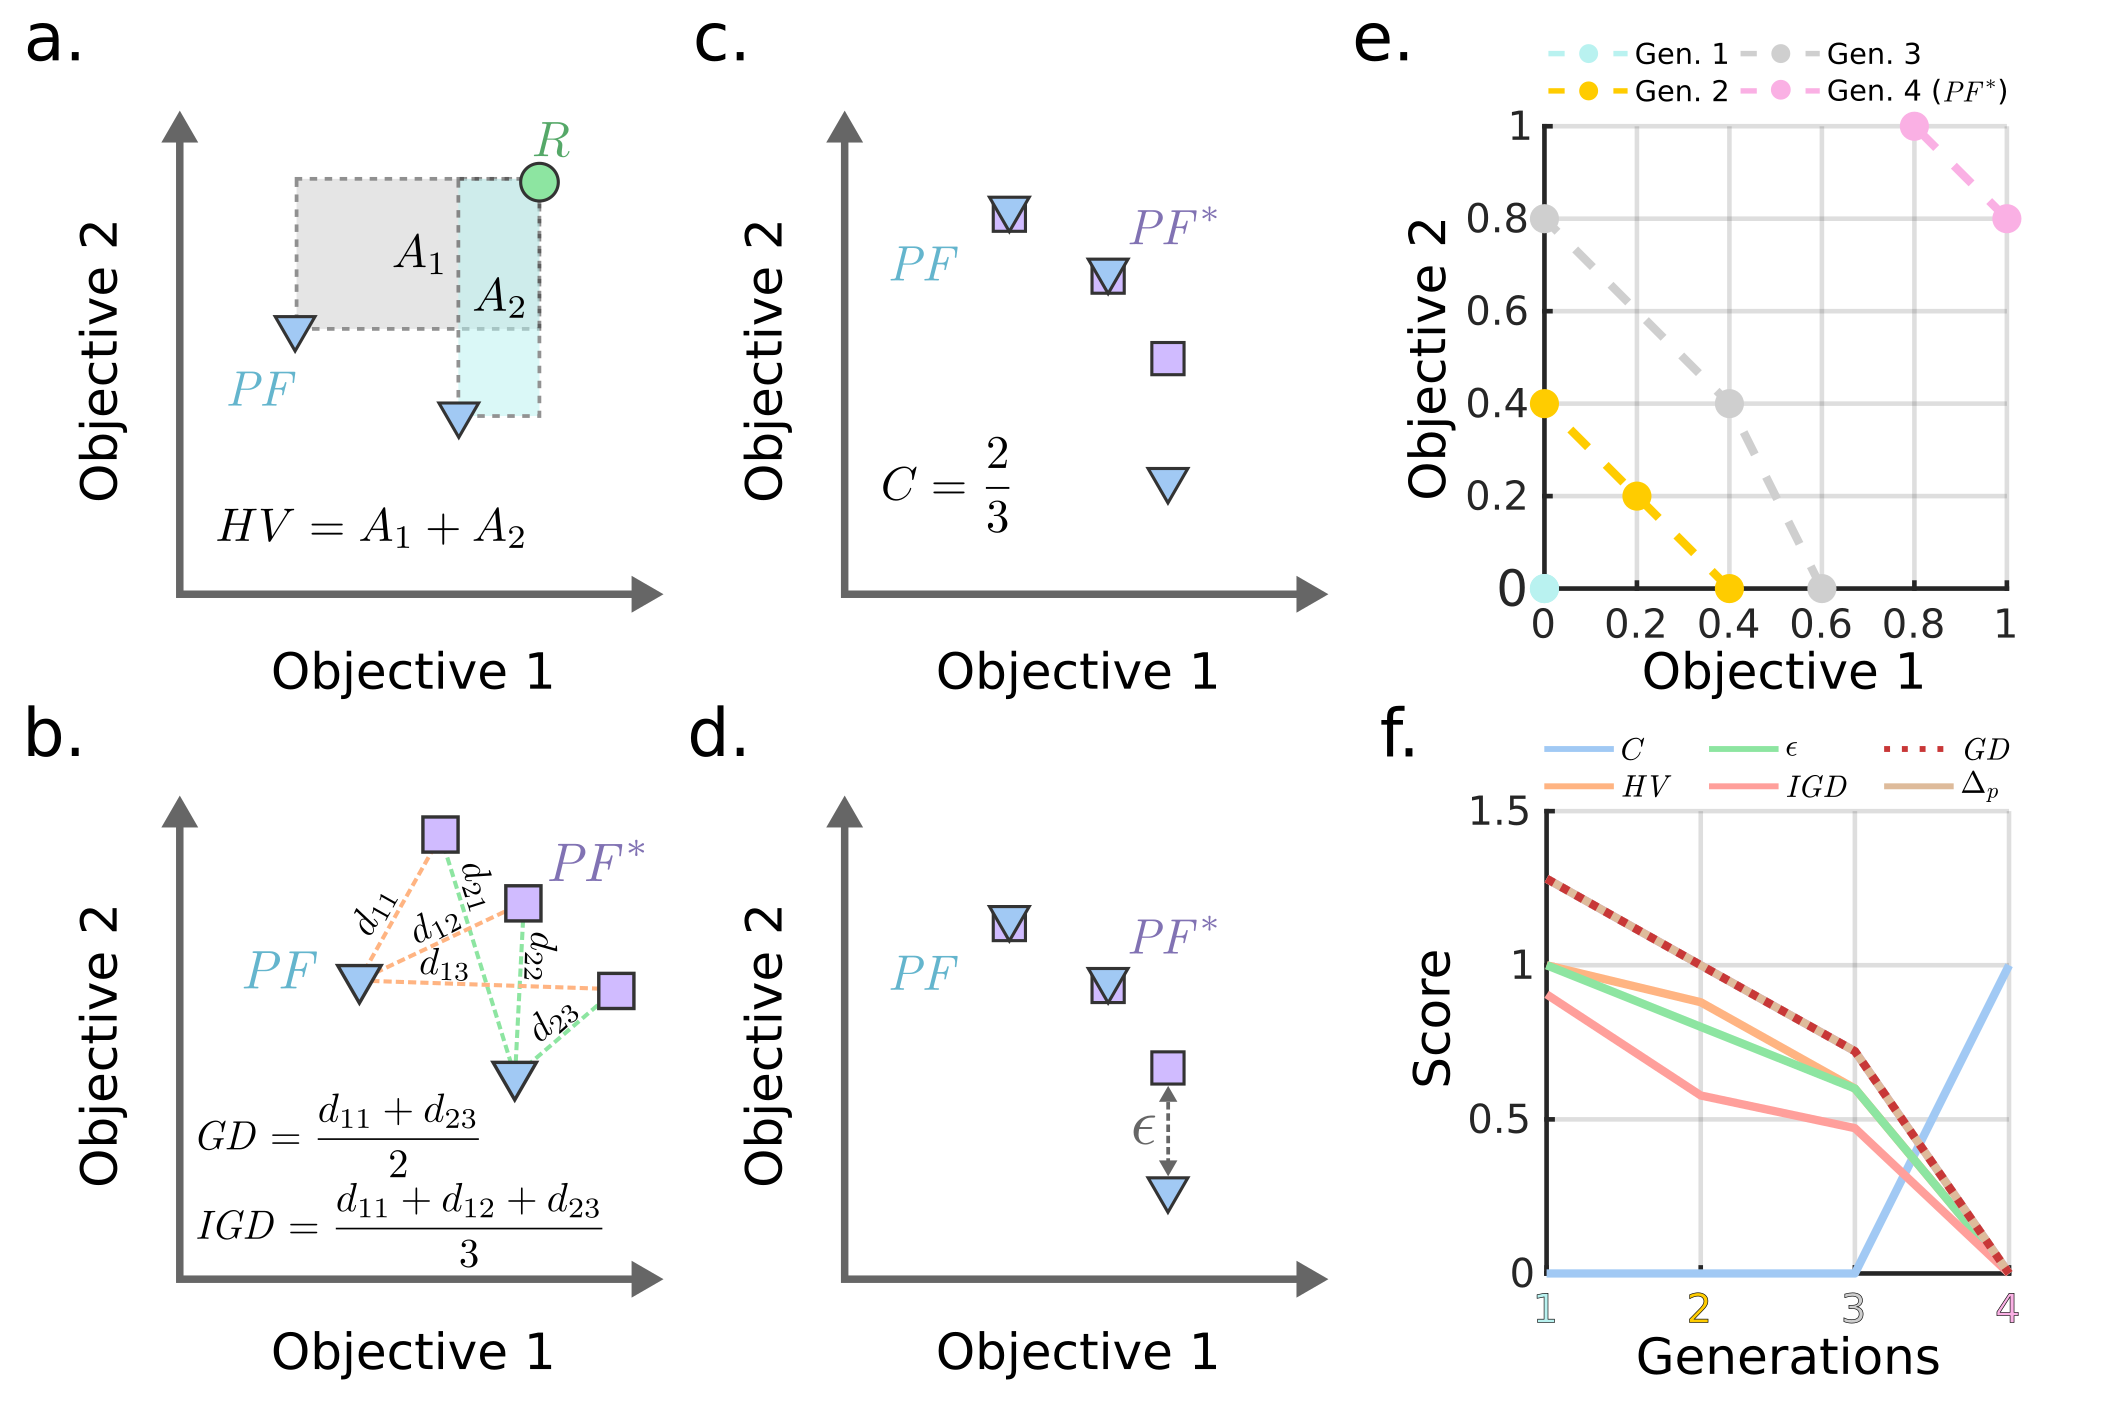
\includegraphics[width=0.8\textwidth,keepaspectratio]{example.png}
    \caption[Conceptual illustration of performance metrics]{(\textbf{a-d}) Conceptual illustration of performance metrics of MOEAs for a two-objectives design problem. $PF$ and $PF^*$ correspond to the Pareto front approximation and the best Pareto front available, respectively. The reference point $R$ must always dominate all solutions in $PF$. (\textbf{e-f}) An example of Pareto fronts with 2 dimensions and associated metrics. The 4th generation corresponds to $\PFs$ used as a reference for comparison.}
\label{fig4:example}
\end{figure}

\subsection{Algorithm parameters}
All parameters used in the simulations of this study were left as default except the following ones. The total number of generations was set to be 200, which was sufficient to reach high quality solutions for the problems of this study. In addition, the population size was set to be 100 for all algorithms unless noted otherwise.  All problems were solved in triplicates with unique random number generator seeds.

\subsection{Metabolic models}
For all simulations, we used a core \textit{E. coli} model, downloaded from the BiGG database (\url{https://bigg.ucsd.edu})  \cite{king2015}, that captures the most important metabolic pathways \cite{palsson2015}.
The product synthesis pathways for each module correspond to native \textit{E. coli} pathways together with well-characterized heterologus pathways for the synthesis of
propanol \cite{tseng2012},
butanol \cite{shen2011},
isobutanol \cite{atsumi2008},
and pentanol \cite{tseng2012}.
The metabolic reactions associated with  these pathways are described in the software implementation (Supplementary Material 1).

\subsection{Implementation} \label{sec:implementation}
The simulations were performed using the ModCell2 software framework \cite{garcia2019}.
The MOEAs are implemented in the PlatEMO Matlab library \cite{tian2017}, except \textit{gamultiobj} which is implemented as part of the Matlab Optimization Toolbox. $HV$ was calculated using the \textit{hv package} \cite{fonseca2006}. All computations were executed in a computer with the Arch Linux operative system, Intel Core i7-3770 processor, and 32 GB of random-access memory. The Matlab 2018b code used to generate the results of this manuscript is available in Supplementary Material 1 and \url{https://github.com/trinhlab/compare-moea}.

\section{Results and Discussion}
\subsection{Case 1: A 3-objectives design problem}
We first formulated a design problem that considers an \textit{E. coli} core model and 3 production modules based on the endogenous acetate, D-lactate, and ethanol biosynthesis pathways (Figure~\ref{fig4:case1}a). We used all MOEAs to solve for the problem by setting the following design parameters: \textit{wGCP} design objective, a maximum number of reaction deletions $\alpha=3$, and no module reactions $\beta=0$.
These design parameters were sufficiently restrictive to generate conflicting objectives.
A total coverage of $\PFs$ ($C=1$)  was reached within 20 generations by several algorithms (Figure~\ref{fig4:case1}b, e, h, i) and by \textit{gamultiobj} after 150 generations (Figure~\ref{fig4:case1}k), while the remaining algorithms could not attain $C$ values above 0.8 (Figure~\ref{fig4:case1}c, d, f, g, j, l). In particular, MaOEADDFC and BiGE obtained the worst $C$, $\epsilon$, and $\Delta_p$ values (Figure~\ref{fig4:case1}m).
Although $C$, $\epsilon$, and $\Delta_p$ values of BiGE indicated inferior performance, this algorithm had the lowest $HV$ since it generated only one point with a high objective value (Figure~\ref{fig4:case1}o).
Due to the simplicity of the problem, every algorithm except MaOEADDFC, tDEA, and BiGE converged to very similar Pareto fronts (Figure~\ref{fig4:case1}n-x), and 5 of them reached $C=1$, indicating convergence to the reference Pareto front (Figure~\ref{fig4:case1}y).

\subsection{Case 2: A 10-objectives design problem}
Using the same model and design parameters as in Case 1, we expanded the number of objectives to represent a more realistic scenario.
These objectives correspond to 6 endogenous pathways for biosynthesis of D-lactate, acetate, ethanol, formate, pyruvate and L-glutamate and 4 heterologous pathways for biosynthesis of propanol, butanol, isobutanol, and pentanol.
The additional objectives increased the difficulty of the problem, leading to more notable difference among algorithm performances (Figure~\ref{fig4:case2}a-k).
The SPEA2SDE algorithm displayed consistent improvement of $C$ as generations progressed, and quickly reached the smallest values of  $\epsilon$ and $\Delta_p$ (Figure~\ref{fig4:case2}h).
Other algorithms, including ARMOEA and MOEAIGDNS, also improved their $\epsilon$ values with the increasing number of generations and reached the same final values of $\epsilon$ and $\Delta_p$ as SPEA2SDE (Figure~\ref{fig4:case2}a, d). However, SPEA2SDE approached $C\cong0.6$, which is twice the value reached by the next best-performing methods (Figure~\ref{fig4:case2}l). Remarkably, SPEA2SDE outperformed every other algorithm in all metrics, except $\HV$. The $\HV$ metric continues to show bias towards algorithms that generated a small number of points and scored poorly in other metrics.


\subsection{Case 3: Use of large population size overcomes poor MOEA performance}
Increasing the number of objectives often leads to a combinatorial explosion of the number of feasible Pareto optimal points and consequently causes poor MOEA performance. This problem can be alleviated by using a larger population size to sample a broader volume of solution space \cite{ishibuchi2009}.
To test this strategy for the 10-objectives design problem above, we increased the population size from 100 to 1000 individuals while all other parameters remained unchanged.
The result showed that
ARMOEA,
MOEAIGDNS,
NSGAII,
SPEA2SDE (the best performer in Case 2),
and \textit{gamultiobj},
could reach $C$ of 0.7, $\epsilon$ of 0, and $\Delta_p$ of 0 in fewer than 50 generations (Figure~\ref{fig4:case3}a, d, g, h, j).
These 5 algorithms also yielded very similar final values across all metrics  (Figure~\ref{fig4:case3}l). The remaining algorithms converged to considerably lower $C$ values (Figure~\ref{fig4:case3}b, c, e, f, i, k).
Remarkably, NSGAII/\textit{gamultiobj}, that is not considered a many-objective solver, performed better than more recent many-objective algorithms such as NSGAIII.

One limitation of using larger populations is an increased cost in computational time. We observed that a 10-fold increase in population sizes resulted in a 10-fold increase in the run times (Figure~\ref{fig4:timing}). Nonetheless, all metrics reached a stable value in the top performing algorithms after 50 generations (out of 200 total), suggesting that fewer generations were needed by using a larger population size.  Among the best performing algorithms with large population sizes, \textit{gamultiobj}, implemented in the Matlab Optimization Toolbox, required the shortest run time, followed by NSGAII and SPEA2SDE implemented in PlatEMO.

\begin{figure}[H]
    \centering
    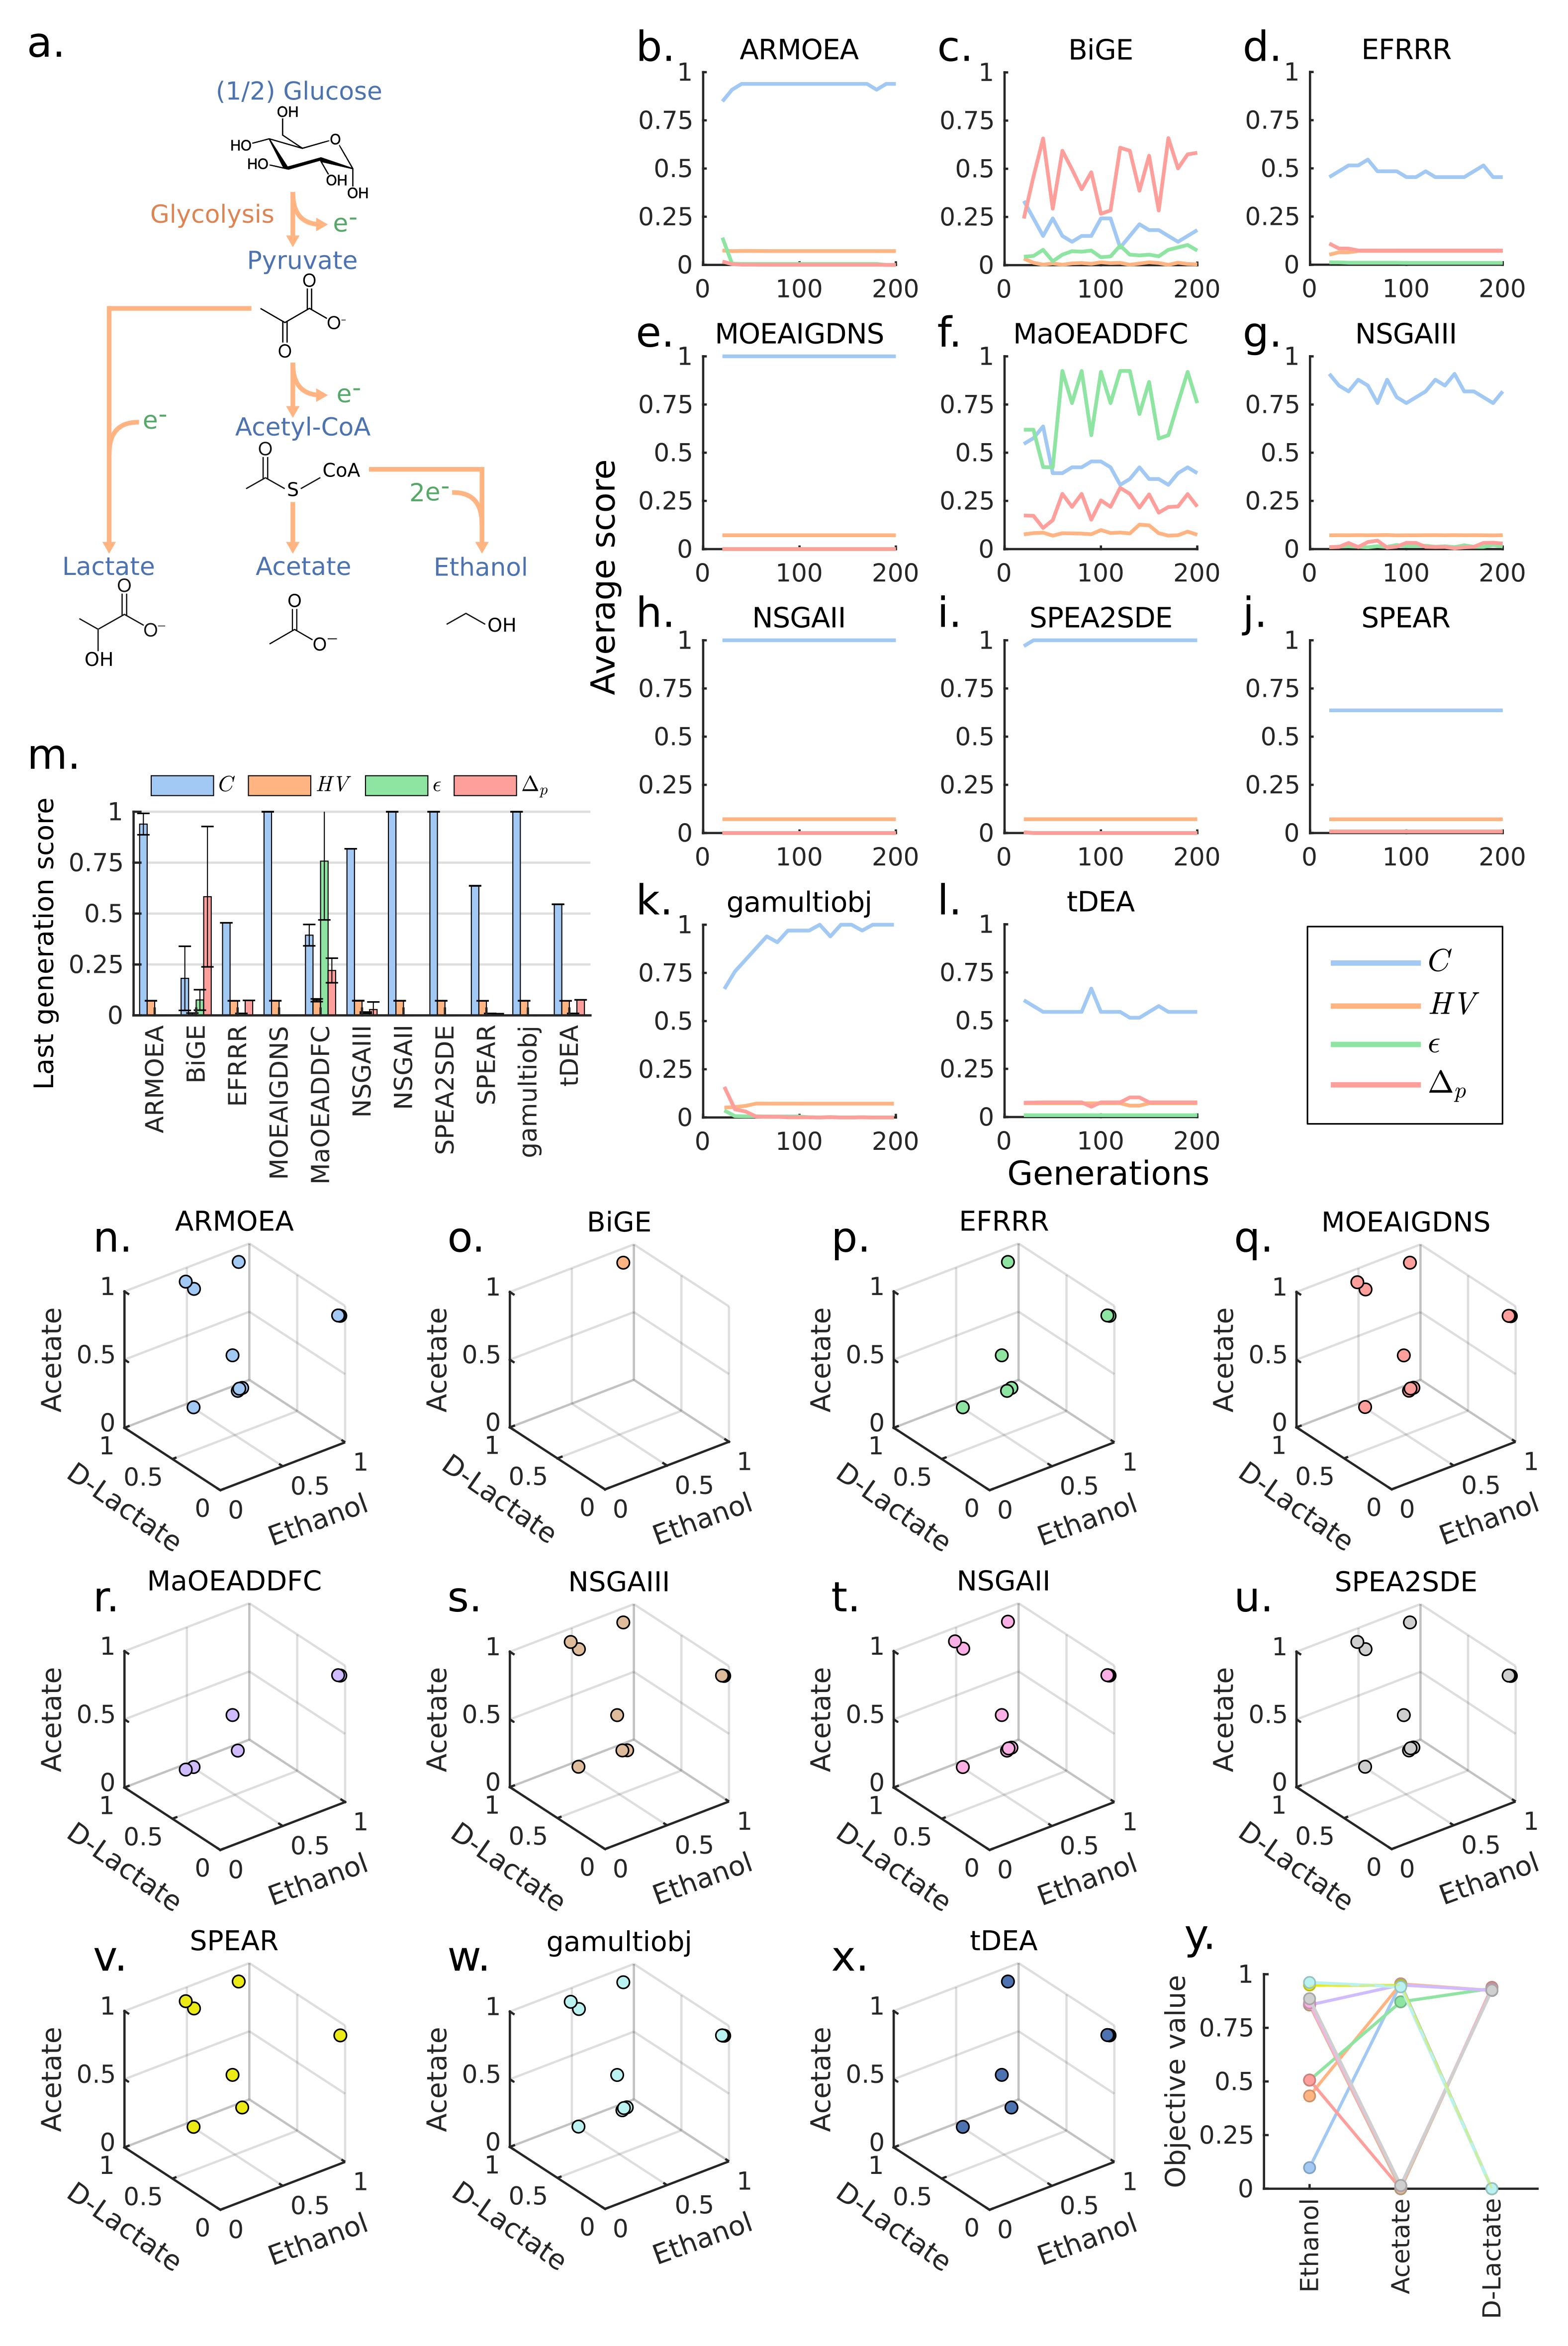
\includegraphics[height=.83\textheight,keepaspectratio]{case1.png}
    %\caption{(Caption next page.)}
    \caption[Comparison of MOEAs for a 3-objectives design problem]{Comparison of MOEAs for a 3-objectives design problem.
	(\textbf{a}) The simplified metabolic pathways for conversion of glucose to the target products. Reducing equivalents are presented with $e^-$.
	(\textbf{b-l}) Generation-dependent performance metrics for various MOEAs.
	(\textbf{m}) Performance metrics for various MOEAs at the last generation.
	(\textbf{n-x}) Pareto fronts of various MOEAs at the last generation. It should be noted that only the first replicate is plotted for clear illustration.
	(\textbf{y}) Reference Pareto front ($\PFs$). Each line represents a solution.}
    \label{fig4:case1}
\end{figure}
%\addtocounter{figure}{-1}
%
%\begin{figure}[t!]
%	\caption{(Previous page.) Comparison of MOEAs for a 3-objectives design problem.
%	(\textbf{a}) The simplified metabolic pathways for conversion of glucose to the target products. Reducing equivalents are presented with $e^-$.
%	(\textbf{b-l}) Generation-dependent performance metrics for various MOEAs.
%	(\textbf{m}) Performance metrics for various MOEAs at the last generation.
%	(\textbf{n-x}) Pareto fronts of various MOEAs at the last generation. It should be noted that only the first replicate is plotted for clear illustration.
%	(\textbf{y}) Reference Pareto front ($\PFs$). Each line represents a solution.}
%\end{figure}

\begin{figure}[H]
    \centering
    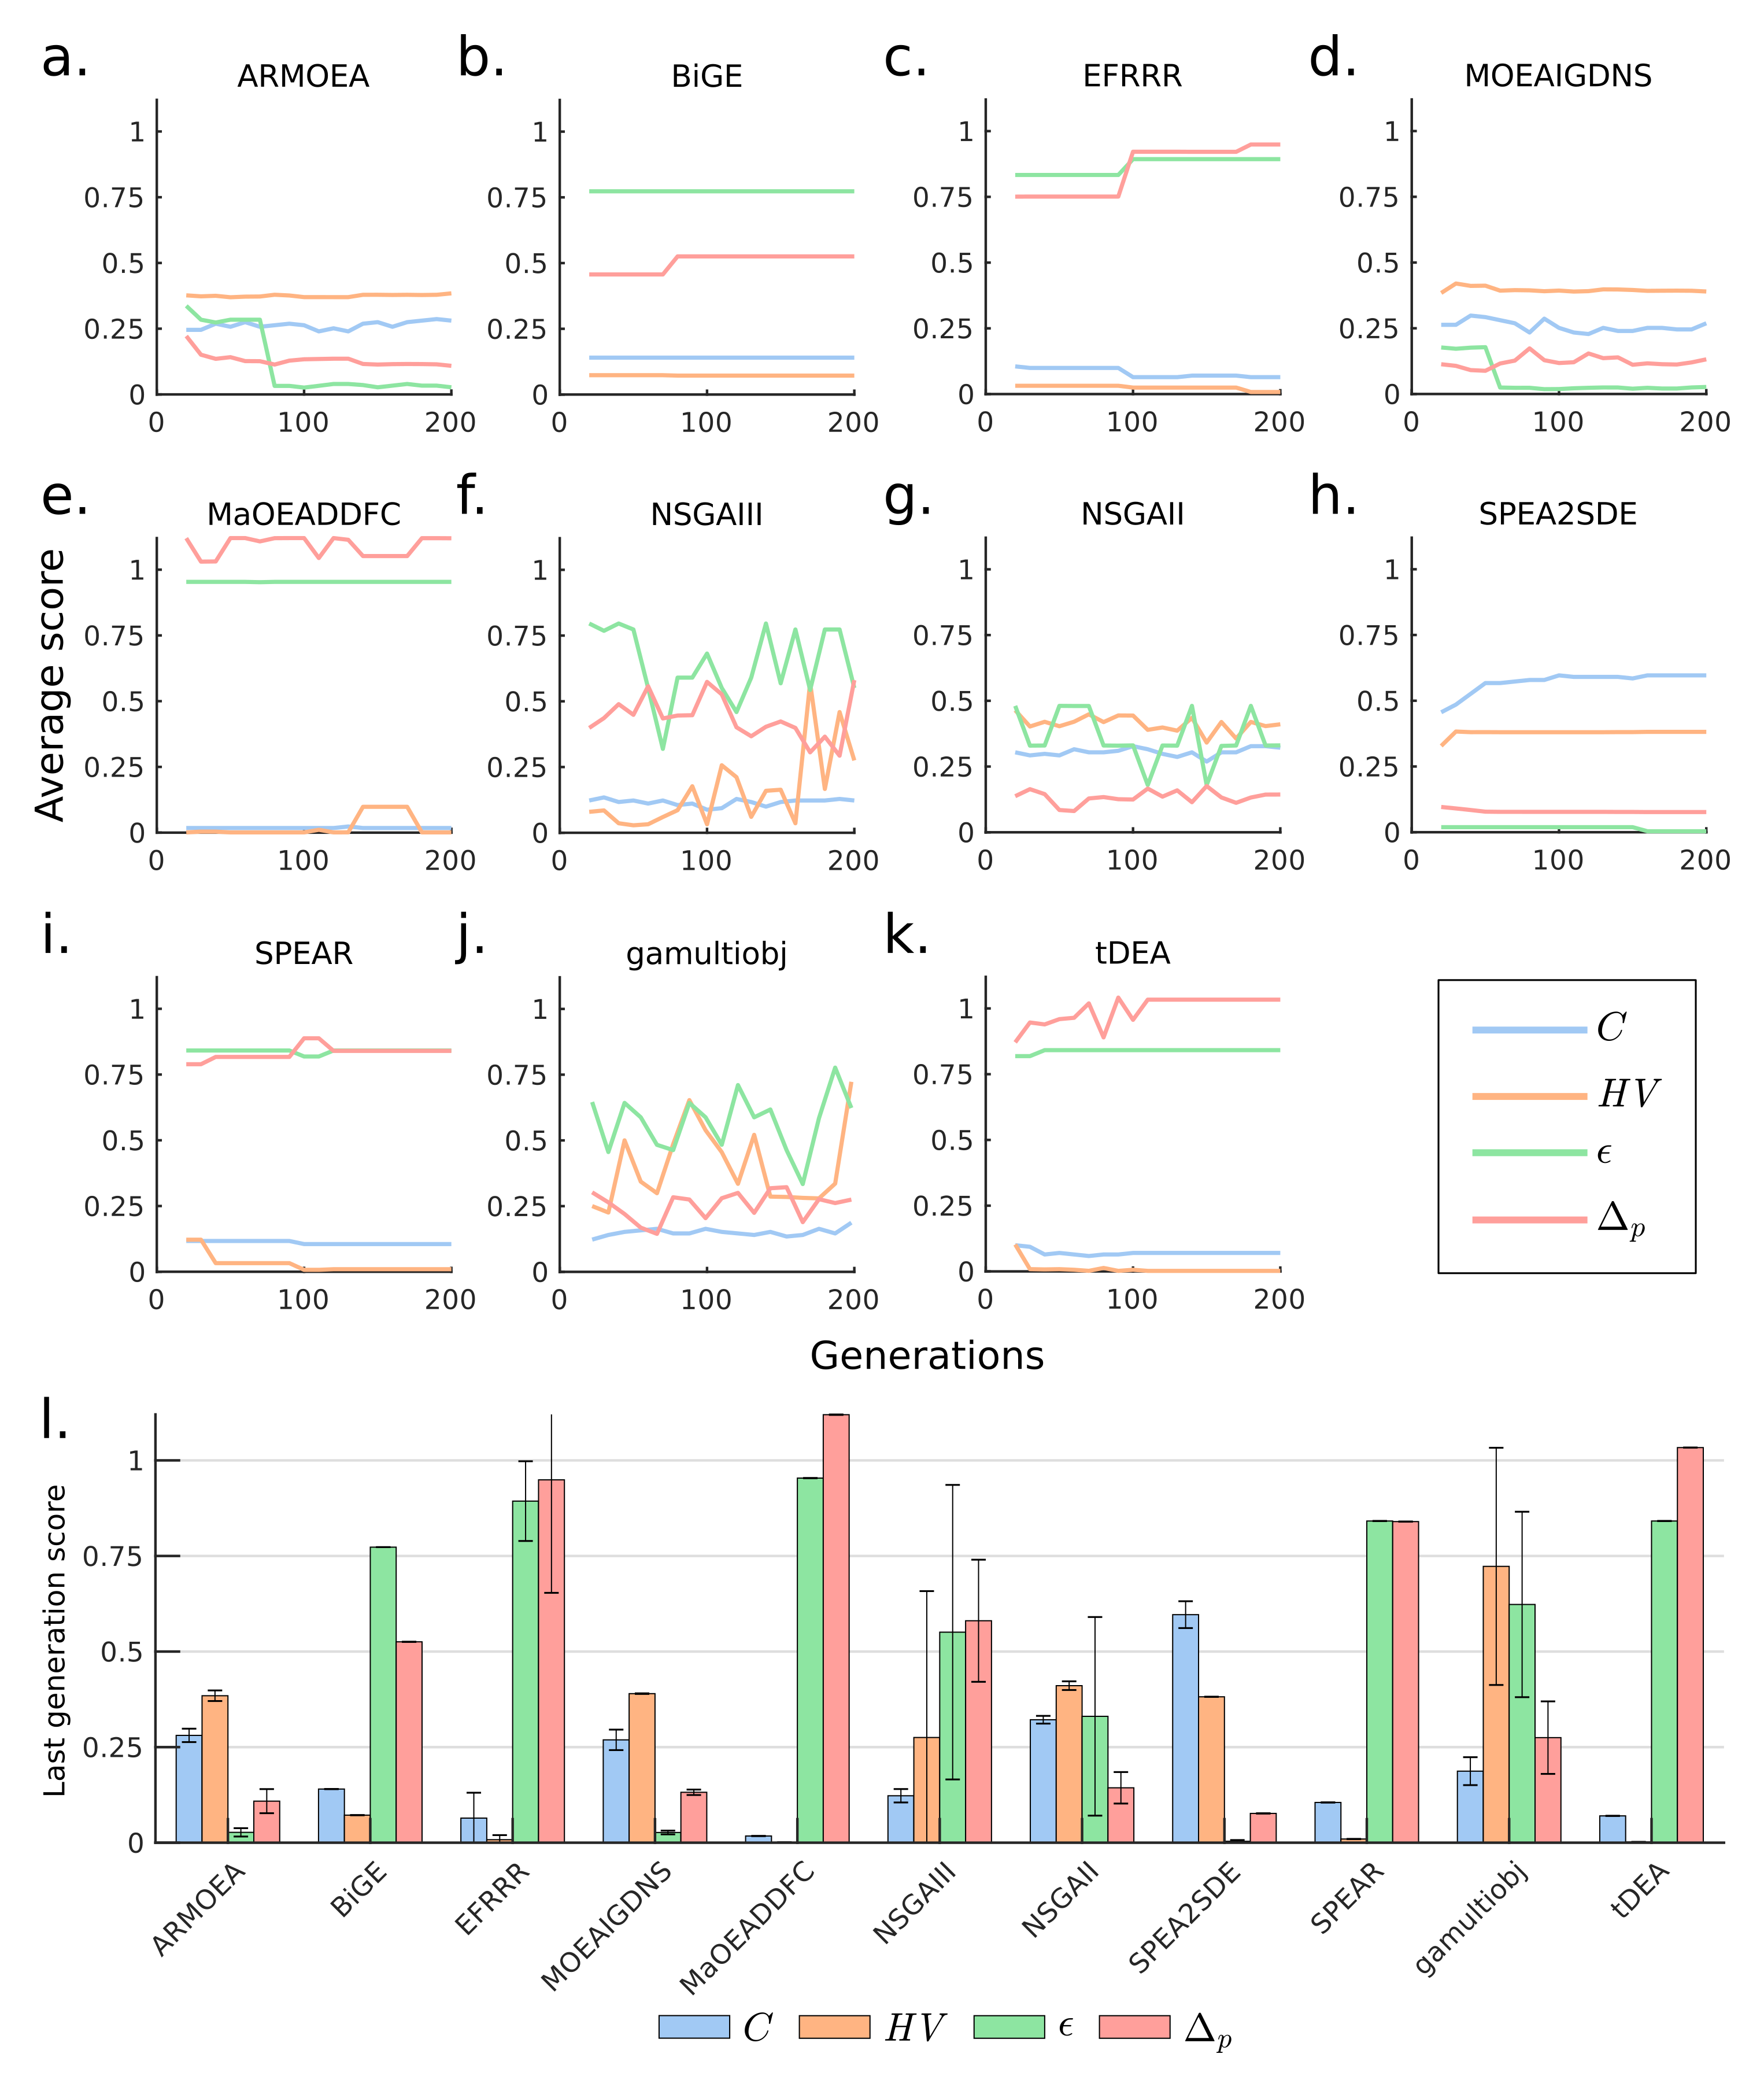
\includegraphics[width=\textwidth,height=\textheight,keepaspectratio]{case2.png}
    \caption[Comparison of MOEAs for a 10-objective design problem]{Comparison of MOEAs for a 10-objective design problem. (\textbf{a-k}) Generation-dependent performance metrics for various MOAEs. (\textbf{l}) Performance metrics for various MOEAs at the last generation.}
\label{fig4:case2}
\end{figure}

\begin{figure}[H]
    \centering
    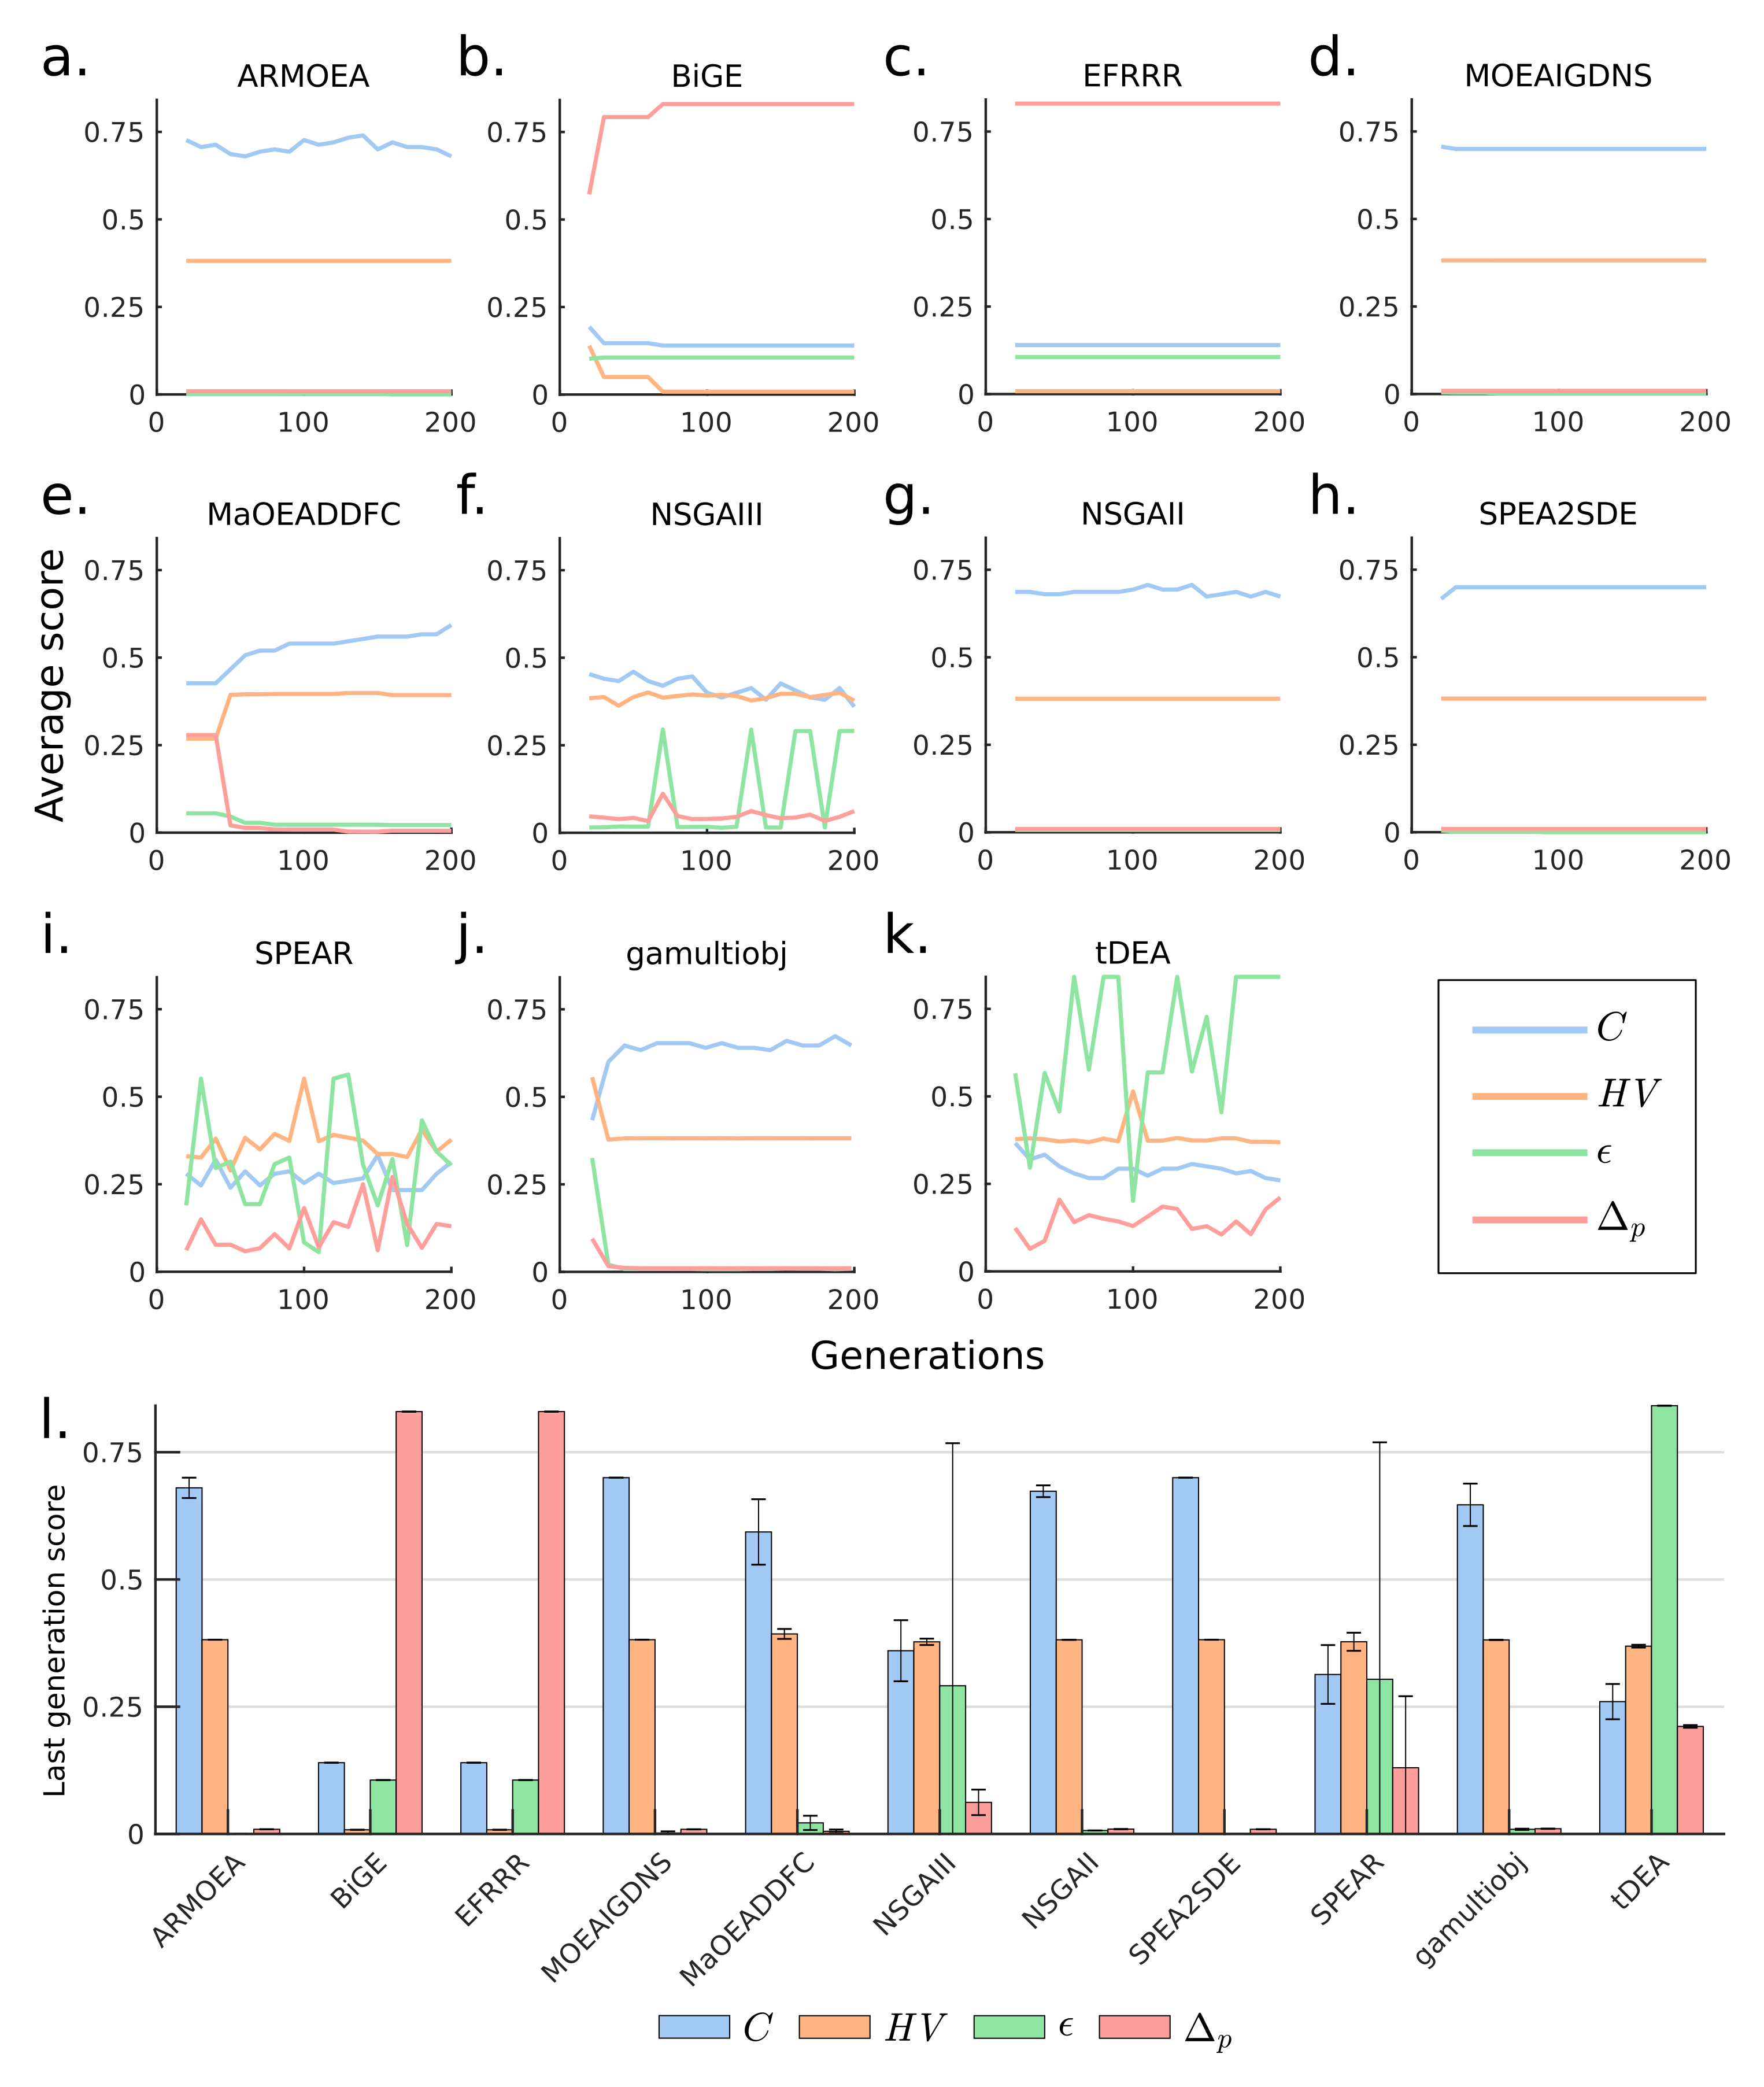
\includegraphics[width=\textwidth,height=\textheight,keepaspectratio]{case3.png}
    \caption[Comparison of MOEAs with increased population sizes]{Comparison of MOEAs for a 10-objectives design problem with larger population sizes
	(\textbf{a-k}) Generation-dependent performance metrics for various MOAEs.	(\textbf{l}) Performance metrics for various MOEAs at the last generation.}
\label{fig4:case3}
\end{figure}

\begin{figure}[H]
    \centering
    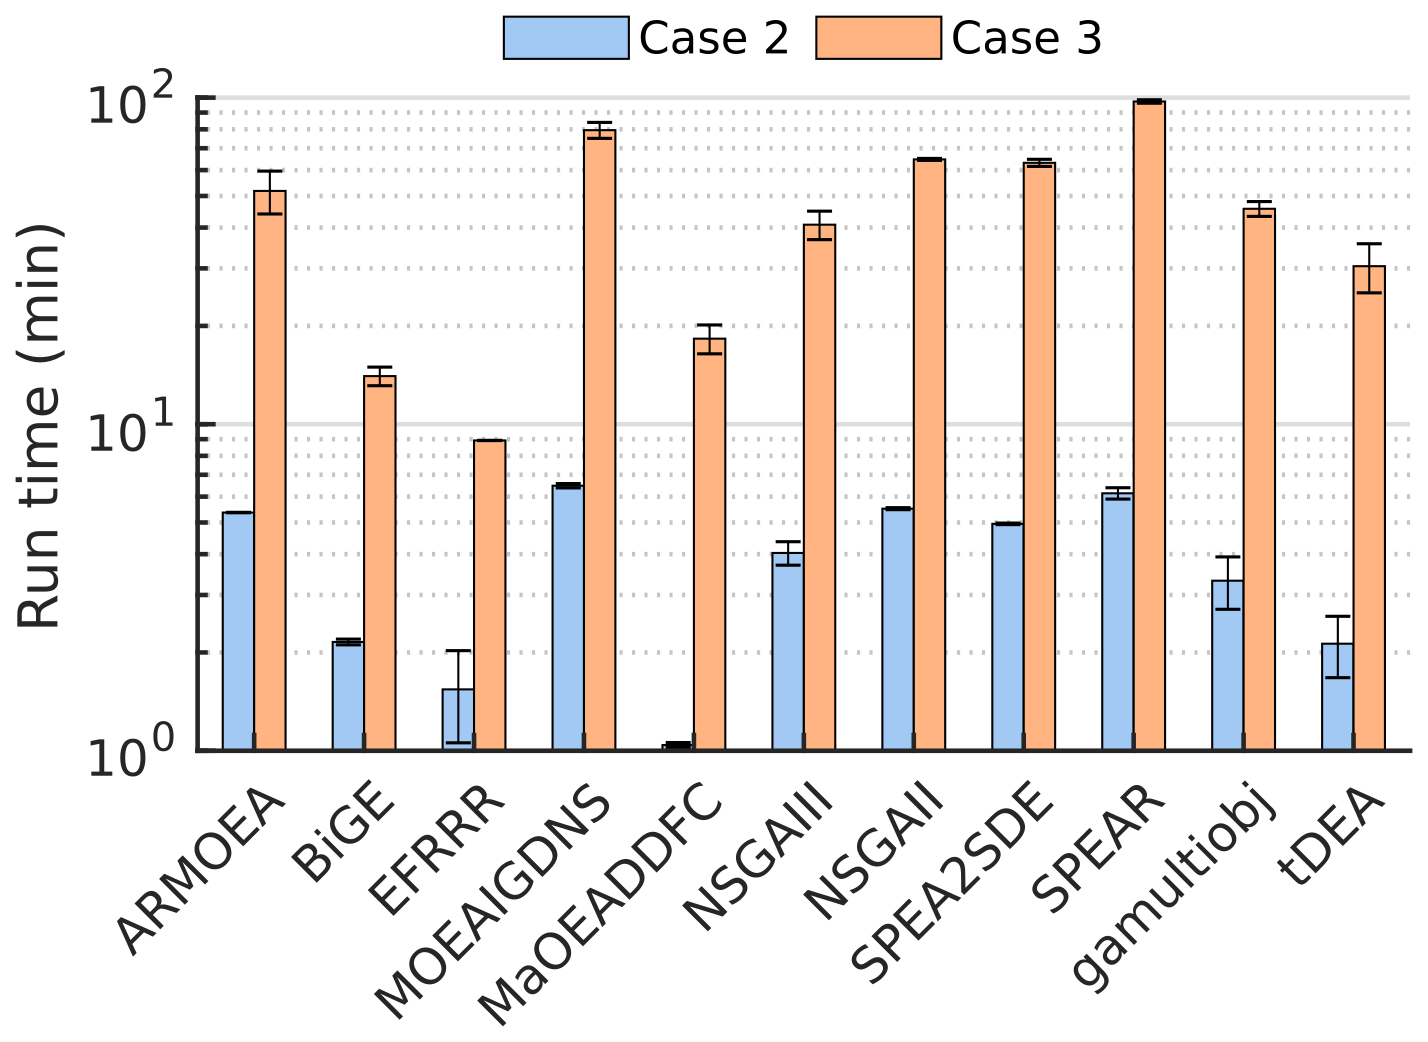
\includegraphics[width=0.45\textwidth,keepaspectratio]{timing.png}
    \caption[Wall-clock run times]{Wall-clock run times for the 10-objectives design problem with population sizes of 100 (Case 2) and 1000 (Case 3).}
\label{fig4:timing}
\end{figure}

%%%%%%%%%%%%%%%%%%%%%%%%%%%%%%%%%%%%%%%%%%

\section{Conclusions}
In this study, we evaluated the performance of several MOEAs to solve the modular cell design problem. SPEA2SDE, the recently developed many-objectives method, was the best performing MOEA for limited population sizes in our study. However, for sufficiently large populations, several algorithms attained the best results, including the well-established NSGAII, which performed better than more recently developed many-objectives MOEAs. We used the most popular performance metrics to compare MOEAs and found that the coverage ($C$) metric is the most valuable indicator. This metric can provide an intuitive quantitative meaning and tends to increase monotonically with the number of generations simulated. In contrast, hypervolume ($\HV$) generally did not differentiate algorithm performance and was misleading in some scenarios where an algorithm generated very few solutions. Overall, these results highlight the need for empirical testing of MOEAs towards specific problems and of the population size as a more important factor in performance than the unique heuristics commonly used by different algorithms.
For the application of modular cell engineering, efficient MOEAs will enable the design of modular cell(s) compatible with many product synthesis modules for large-scale metabolic networks and the identification of more diverse and better solutions that will provide more viable options for practical implementation.

%%%%%%%%%%%%%%%%%%%%%%%%%%%%%%%%%%%%%%%%%%





%%%%%%%%%%%%%%%%%%%%%%%%%%%%%%%%%%%%%%%%%%
%\vspace{6pt}

%%%%%%%%%%%%%%%%%%%%%%%%%%%%%%%%%%%%%%%%%%
%% optional
%\supplementary{The following are available online at \linksupplementary{s1}, Figure S1: title, Table S1: title, Video S1: title.}

% Only for the journal Methods and Protocols:
% If you wish to submit a video article, please do so with any other supplementary material.
% \supplementary{The following are available at \linksupplementary{s1}, Figure S1: title, Table S1: title, Video S1: title. A supporting video article is available at doi: link.}

%%%%%%%%%%%%%%%%%%%%%%%%%%%%%%%%%%%%%%%%%%
%\authorcontributions{conceptualization, S.G. and C.T.; methodology, S.G.; software, S.G.; validation, S.G.; formal analysis, S.G.; investigation, S.G.; resources, S.G.; data curation, S.G.; writing--original draft preparation, S.G.; writing--review and editing, S.G. and C.T.; visualization, S.G. and C.T.; supervision, C.T.; project administration, C.T.; funding acquisition, C.T.}
%\authorcontributions{CTT initiated and supervised the study. SG and CTT designed experiments. SG performed simulation experiments and analyzed data. SG and CTT wrote and approved the manuscript.}

%%%%%%%%%%%%%%%%%%%%%%%%%%%%%%%%%%%%%%%%%%
%\funding{Please add: ``This research received no external funding'' or ``This research was funded by NAME OF FUNDER grant number XXX.'' and  and ``The APC was funded by XXX''. Check carefully that the details given are accurate and use the standard spelling of funding agency names at \url{https://search.crossref.org/funding}, any errors may affect your future funding.}
%\funding{This research was funded by the NSF CAREER Award (NSF\#1553250) and the Center of Bioenergy Innovation (CBI), U.S. Department of Energy Bioenergy Research Center supported by the Office of Biological and Environmental Research in the DOE Office of Science. The views, opinions, and/or findings contained in this article are those of the authors and should not be interpreted as representing the official views or policies, either expressed or implied, of the funding agencies.}

%%%%%%%%%%%%%%%%%%%%%%%%%%%%%%%%%%%%%%%%%%
%\acknowledgments{In this section you can acknowledge any support given which is not covered by the author contribution or funding sections. This may include administrative and technical support, or donations in kind (e.g., materials used for experiments).}

%%%%%%%%%%%%%%%%%%%%%%%%%%%%%%%%%%%%%%%%%%
%\conflictsofinterest{The authors declare no conflict of interest.}

    \chapter{Development of linear formulations to solve the modular cell problem and application to design a universal modular cell} \label{ch:milp}

\disclose{Harnessing natural modularity of cellular metabolism to design a modular chassis cell for a diverse class of products by using goal attainment optimization. Garcia, S., and Trinh, C. T. In review, 2020} Supplementary Files S1 and S2 are provied as attachments.

\newcommand*\mycommand[1]{\texttt{\emph{#1}}}

\section*{Abstract}
Modular design is key to achieve efficient and robust systems across engineering disciplines. Modular design potentially offers advantages to engineer microbial systems for biocatalysis, bioremediation, and biosensing, overcoming the slow and costly design-build-test cycles in the conventional cell engineering approach. These systems consist of a modular cell chassis compatible with modules that enable programmed functions such as overproduction of a desirable chemical. We previously proposed a multi-objective optimization framework coupled with metabolic flux models to design modular cells and solved it using multi-objective evolutionary algorithms. However, such approach might not achieve solution optimality and hence limit design options for experimental implementation. In this study, we developed the goal attainment formulation compatible with optimization algorithms that guarantee solution optimality. We applied goal attainment to design an \textit{Escherichia coli} modular cell capable of synthesizing all molecules in a biochemically diverse library at high yields and rates with only a few genetic manipulations. To elucidate modular organization of the designed cells, we developed a flux variance clustering (FVC) method by identifying reactions with high flux variance and clustering them to identify metabolic modules. Using FVC, we identified reaction usage patterns for different modules in the modular cell, revealing its broad pathway compatibility is enabled by the natural modularity and flexible flux capacity of endogenous core metabolism. Overall, this study not only sheds light on modularity in metabolic networks from their topology and metabolic functions but also presents a useful synthetic biology toolbox to design modular cells with broad applications.


\section{Introduction}

Microbial metabolism can be engineered to produce a large space of molecules from renewable and sustainable feedstocks \citep{lee2019}.
Currently, only a handful of fuels and chemicals out of the many possible molecules offered by nature are industrially produced by microbial conversion, mainly because the strain engineering process is too laborious and expensive \citep{nielsen2016}.
To overcome this roadblock and produce a more diverse range of molecules requires innovative technologies for rapid and economically competitive strain engineering \citep{trinh2016, nielsen2016, lee2019}.
The principles of modular design that have shown great success in traditional engineering disciplines can be adapted to construct modular cell biocatalysts in a plug-and-play fashion with minimal strain design-build-test cycles \citep{garcia2019b}.

Multi-objective optimization is a powerful mathematical framework widely applied in engineering disciplines to tackle the optimal design of a complex system with multiple conflicting objectives \citep{coello2004, rangaiah2009}.
This framework has recently been used to design modular systems in conventional  engineering \citep{helmer2010}, and to explain the modularity of natural biological systems that enable cellular robustness and adaptability \citep{kitano2004, kashtan2007, clune2013, shoval2012, schuetz2012}.
Using multi-objective optimization, microbial metabolism can be redirected to generate modular production strains that are systematically assembled from an engineered modular cell and exchangeable production modules, where each module synthesizes a target molecule \citep{garcia2019}. This modular cell design approach, known as ModCell2, uses the principles of mass balance and thermodynamics of biochemical reaction networks to predict metabolic fluxes upon genetic manipulations \citep{garcia2019, garcia2019c}.
Based on such flux predictions, a multi-objective optimization problem is then formulated and solved with a multi-objective evolutionary algorithm (MOEA)\citep{zhou2011,deb2002} to yield a sample of the Pareto front (i.e., the set of optimal solutions to the problem with minimal trade-offs among objectives) that a designer can explore genetic manipulation targets for modular cell engineering.

In this study, we developed ModCell2-MILP, a ModCell2-based formulation to be compatible with mixed integer linear programming (MILP) algorithms. This framework presents a significant advancement from ModCell2 in solving the multi-objective strain design problem for modular cell engineering. Specifically, ModCell2-MILP is developed to (i) guarantee optimal solutions, (ii) completely enumerate alternative solutions of a target design, and (iii) describe practical engineering goals more directly (e.g., design of a modular cell where all production modules lead to a product yield above 50\% of the theoretical maximum). By applying ModCell2-MILP to analyze the genome-scale metabolic network of \textit{Escherichia coli}, we could identify a universal modular cell that is compatible with a diverse class of production modules. To gain a mechanistic view into the modular organization of metabolic networks, we developed a flux variance clustering (FVC) method by identifying reactions with high flux variance and clustering them to identify metabolic modules. Using FVC, we found that broad pathway compatibility of the modular cell is facilitated by its natural modularity and flexible flux capacity of endogenous core metabolism. We anticipate ModCell2-MILP and FVC can serve as powerful tools for not only elucidating natural and synthetic metabolic modularity but also rationally designing modular cells for broad biotechnological applications in biocatalysis, bioremediation, and biosensing.

\section{Materials and methods}
\subsection{Modular cell design}
\subsubsection{Design principles}

ModCell design enables rapid assembly of production strains with desirable phenotypes from a modular (chassis) cell \citep{trinh2015, garcia2019, garcia2019b}.
More specifically, a modular cell contains core metabolic pathways shared among production modules (Figure~\ref{fig5:modcell}a).
The chassis interfaces with the modules through enzymatic and genetic synthesis machinery and precursor metabolites (Figure~\ref{fig5:modcell}b).
Modules contain auxiliary regulatory and metabolic pathways (Figure~\ref{fig5:modcell}c) that enable a desired phenotype for optimal biosynthesis of a target molecule, for example, \emph{weak growth coupled to product formation} (\textit{wGCP}), where a positive correlation between growth and product synthesis rates is enforced (Figure~\ref{fig5:modcell}d) \citep{burgard2003, klamt2015, garcia2019}.
The \textit{wGCP} phenotype is useful because it enables rapid pathway optimization by adaptive laboratory evolution \citep{fong2005, trinh2009b} or high-throughput genetic library selection \citep{garst2017}.
The design objective phenotypes are determined from cellular growth and product synthesis rates based on steady-state stoichiometric metabolic models \citep{palsson2015}. A modular cell is said to be \emph{compatible} with a module if the design objective of the resulting production strain is above a specified threshold.
The different biochemical nature of production modules to synthesize target metabolites can make the design objectives compete with each other and also the cellular objectives (e.g., biomass formation) compete with the engineering objectives (e.g., product formation), turning the ModCell design problem into a multi-objective and multi-level optimization problem.

%\afterpage{%
\begin{figure}[p]
    \centering
    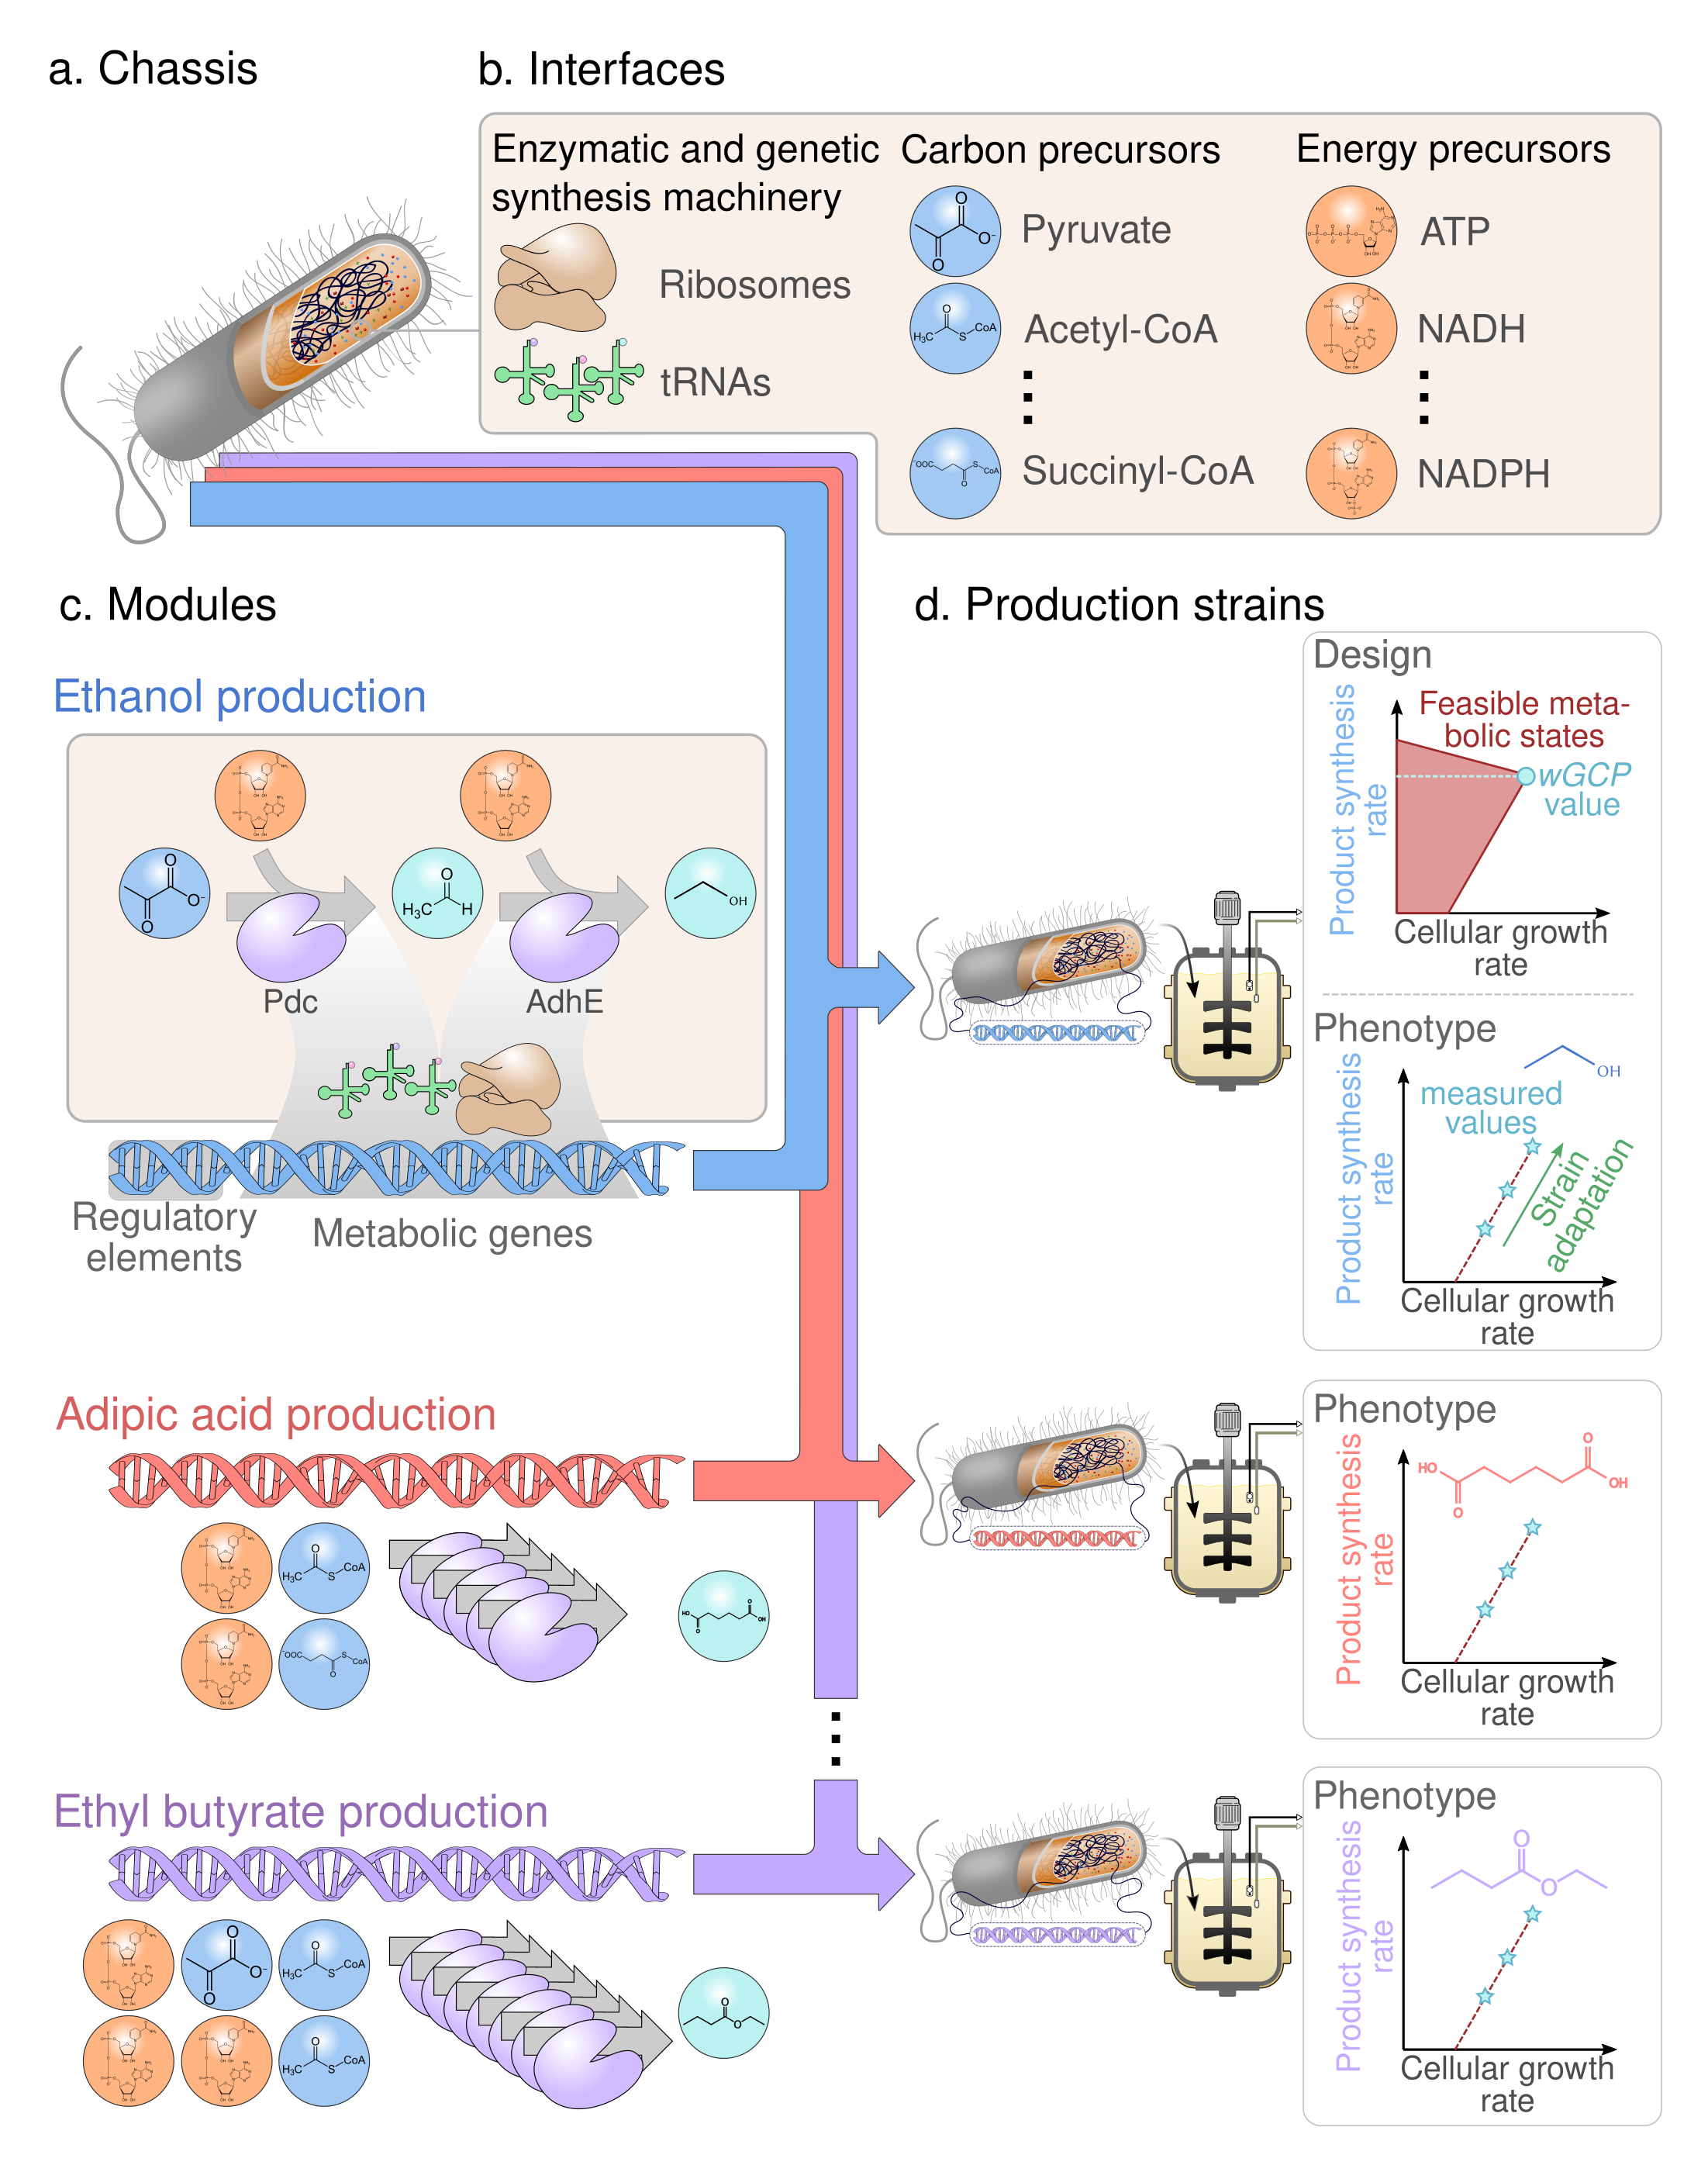
\includegraphics[width=\textwidth,height=.8\textheight,keepaspectratio]{modcell.png}
    \caption[Principles of modular cell design]{Principles of modular cell design. (a) Modular cell chassis. (b) Interfaces. (c) Production modules. (d) Production strains. A modular cell is designed to provide the necessary precursors for biosynthesis pathway modules that are independently assembled with the modular cell to generate production strains exhibiting desirable phenotypes. The \textit{wGCP} phenotype, one of the possible design objectives, enforces the coupling between the desirable product synthesis rate and the maximum cellular growth rate.}
    \label{fig5:modcell}
\end{figure}
%}

\subsubsection{Multi-objective optimization formulation}
The modular cell design problem is stated as a general multi-objective optimization problem of the form:
\begin{equation}
\underset{x}{\text{max}} \quad  F(x) = (f_{1}(x), f_{2}(x), \ldots, f_K (x))^\top  \quad  \text{s.t. } x \in X \label{eq5:multiobj}
\end{equation}
\noindent where $f_k$ is the desirable phenotype for production module $k$, $x$ are the problem variables including binary design variables corresponding to genetic manipulations, and $X$ is the set of constraints including mass balance of metabolism. Optimal solutions for the multi-objective optimization problem \eqref{eq5:multiobj} are defined using the concept of domination: A vector $a=(a_1,\dots,a_K)^\top$ \textit{dominates} another vector $b=(b_1,\dots ,b_K)^\top$, denoted as  $a\prec b$, if and only if $a_i\ge b_i \; \forall i\in\{1,2,\dots,K\}$ and $a_i\ne b_i$ for at least one $i$. A feasible solution $x^* \in X$ of the multi-objective optimization problem is called a Pareto optimal solution if and only if  there does not exist a vector $x'\in X$ such that $F(x')\prec F(x^*)$. The set of all Pareto optimal solutions is called Pareto set:
\begin{equation}
\mathit{PS}:=\{x \in X:\nexists \, x' \in X, F(x') \prec F(x)\}
\end{equation}
The projection of the Pareto set in the objective space is denoted as Pareto front:
\begin{equation}
\mathit{PF}:=\{F(x): x \in PS \}
\end{equation}
Different feasible points in $\mathit{PS}$ (i.e., different genetic manipulations) which map to a single point in $\mathit{PF}$ (i.e., the same phenotype) are denoted \textit{alternative solutions}.

The design variables $x$ in ModCell2 correspond to chassis reaction deletions, that remove undesired metabolic functions,  and module reaction insertions, that allow to identify optimal module configurations without extensive prior knowledge of the product synthesis pathway.  The constraint set $X$ is comprised of two types: (i) flux simulation constraints (e.g., mass balance,  reaction reversibility, and flux bound) that allow to predict fluxes in the design objectives upon genetic manipulations, and (ii) implementation constraints that involve the maximum number of reaction deletions in the chassis (denoted by $\alpha$) and the maximum number of module reaction insertions per module (denoted by $\beta$). The following sections describe the problem formulation in detail using the definitions compiled in the Definitions Section.

\subsubsection{Design objectives} \label{sec:do}

Design objectives, $f_k$, that correspond to specific metabolic phenotypes within the space of feasible steady-state reaction fluxes, $\Pi_{km}$, of production network $k$ (i.e., the combination of the chassis network with the production module $k$) and metabolic state $m$, are defined as follows:
\begin{alignat}{2}
		& \Pi_{km}(e_{jk}):=\{v_{jkm}\in\mathbb{R}: \\
		&	\sum_{j\in \mathcal{J}_k} S_{ijk} v_{jkm} =0  && \forall i\in \mathcal{I}_k 		\label{eq5:pi_mass_bal}\\
		& l_{jkm} e_{jk}  \le v_{jkm} \le e_{jk} u_{jkm} \;  && \forall j\in \mathcal{J}_k 			\label{eq5:pi_bound}%\\
\end{alignat}
\noindent Here, $v_{jkm}$ is the rate (mmol/gCDW/hr) of reaction $j$ in production network $k$ under metabolic state $m$.
Constraint \eqref{eq5:pi_mass_bal} enforces mass balance for all metabolites according to reaction stoichiometry given by the coefficients $S_{ijk}$, and constraint \eqref{eq5:pi_bound} imposes bounds, $l_{jkm}$ and $u_{jkm}$, for the metabolic fluxes according to reaction reversibility, experimentally measured values, and specified metabolic state.
The binary variable $e_{jk}$ is used in the overall optimization problem to indicate whether reaction $j$ in production network $k$ is removed and thus cannot carry any flux. Two metabolic states $m$ are considered, growth and non-growth, denoted $\mu$  and $\bar{\mu}$, respectively. These states are differentiated by their   flux bounds $l_{jkm}$ and $u_{jkm}$. For growth state, the lower bound of the biomass formation reaction that represents cell division, $v_{Xkm}$, is set to a minimum value of  $\gamma$, i.e., $l_{Xk\mu} = \gamma \; (\forall k \in \mathcal{K}$), while there is no upper limit to growth, i.e., $u_{Xk\mu} = \infty \; (\forall k \in \mathcal{K}$).
On the other hand, for the non-growth state both bounds are set to 0, i.e., $l_{Xk\bar{\mu}} = 0 \text{ and } u_{Xk\bar{\mu}}= 0 \; (\forall k \in \mathcal{K}$).

Given the feasible metabolic flux space, $\Pi_{km}$, the following design objectives, based on the product synthesis rate reaction, $v_{Pkm}$, are of interest:
\begin{alignat}{3}
	f_k^{wGCP} & =\frac{v_{Pk\mu}}{v_{Pk\mu}^{max}}\in[0,1], \qquad & & \forall k\in \mathcal{K} \label{eq5:obj_wgcp}\\
	f_k^{lsGCP} & =b_{\mu} \frac{v_{Pk \mu}}{v_{Pk\mu}^{max}} \, + b_{\bar{\mu}} \frac{v_{Pk \bar{\mu}}}{v_{Pk\bar{\mu}}^{max}} \in[0,b_{\mu}+b_{\bar{\mu}}], \quad  & &  \forall k\in \mathcal{K} \label{eq5:obj_lsgcp}\\
	f_k^{NGP} & = \frac{v_{Pk \bar{\mu}}}{v_{Pk\bar{\mu}}^{max}} \in[0,1], \qquad  & &  \forall k\in \mathcal{K} \label{eq5:obj_ngp}
\end{alignat}
\noindent
The product synthesis fluxes, including $v_{Pk\mu}$, $v_{Pk\mu}^{max}$, $v_{Pk\bar{\mu}}$, and $v_{Pk\bar{\mu}}^{max}$, are computed by solving the following linear programming problems:
\begin{alignat}{3}
& v_{Pk\mu} 	&\in& \,	\text{arg }	\underset{}{\text{max}} \{v_{Xk\mu}-\epsilon \, v_{Pk\mu} : v_{k\mu}\in \Pi_{k\mu}(e_{jk})	\} \label{eq5:vpgLP}	\\
& v_{P k\mu}^{max} &\in& \,	\text{arg }	\underset{}{\text{max}} \{v_{Pk \mu} : v_{k \mu} \in \Pi_{k \mu} (e_{jk} = 1, \; \forall j\in \mathcal{J}_k) 	\}   \label{eq5:vpmaxLP_g}	\\
& v_{Pk \bar{\mu}} 	&\in& \,	\text{arg }	\underset{}{\text{min}} \{v_{Pk \bar{\mu}} : v_{k \bar{\mu}} \in \Pi_{k \bar{\mu}}(e_{jk})\} \label{eq5:vpngLP} \\
& v_{Pk\bar{\mu}}^{max} &\in& \,	 \text{arg }	\underset{}{\text{max}} \{v_{Pk \bar{\mu}} : v_{k \bar{\mu}} \in \Pi_{k \bar{\mu}}(e_{jk} = 1, \; \forall j\in \mathcal{J}_k)\}  \label{eq5:vpmaxLP_ng}
\end{alignat}
\noindent
The maximum product synthesis fluxes \eqref{eq5:vpmaxLP_g} and \eqref{eq5:vpmaxLP_ng} used for objective scaling are only calculated once by not using any deleted reactions ($e_{jk}=1$), while the target phenotype fluxes \eqref{eq5:vpgLP} and \eqref{eq5:vpngLP} are functions of the deleted reactions $e_{jk}$. The design objectives, \textit{wGCP} \eqref{eq5:obj_wgcp}, \textit{lsGCP} \eqref{eq5:obj_lsgcp}, and \textit{NGP} \eqref{eq5:obj_ngp}, were previously proposed \citep{garcia2019} and briefly described here. The weak growth coupled to product formation objective (\textit{wGCP}) \eqref{eq5:obj_wgcp} seeks to maximize the minimum product rate at the maximum cellular growth, which is accomplished by a titled objective function\citep{feist2010} \eqref{eq5:vpgLP}. The linearized strong growth coupled to product formation (\textit{lsGCP}) \eqref{eq5:obj_lsgcp} objective seeks to maximize the minimum product synthesis rate at the non-growth state $v_{Pk\bar{\mu}}$ in addition to the goal of \textit{wGCP}. Finally, the non-growth production (\textit{NGP}) \eqref{eq5:obj_ngp} objective seeks to optimize the minimum product synthesis rate during the non-growth state.


\subsubsection{Design constraints} \label{sec:problem_constraints}
All the constraints of the modular cell design problem are gathered as follows:
\begin{alignat}{2}
& \mathrlap{	 \Omega:=\{f'_k \in \mathbb{R}, \, y_j, z_{jk}, d_{jk}, w_{k}, e_{jk} \in \, \{0,1\} : }\\ %
& \sum_{j\in \mathcal{C}} (1-y_j)\le \alpha 						\label{eq5:acon}\\
& \sum_{j\in \mathcal{C} - \mathcal{N}_k }z_{jk} \le \beta_k & \forall k\in \mathcal{K} 	\label{eq5:bcon}\\
& z_{jk}\le 1-y_j  & \forall j\in \mathcal{C} - \mathcal{N}_k , \;  k\in \mathcal{K}	\label{eq5:yzcon}\\
& d_{jk} = y_j \lor z_{jk} & \forall j \in \mathcal{C} ,\;  k \in \mathcal{K} \label{eq5:d_def}\\
& f'_k = f_k w_k & \forall k \in \mathcal{K} \label{eq5:fprime}\\
& e_{jk} = (d_{jk} \land w_k) \lor \lnot w_k & \forall j \in \mathcal{C} ,\;  k \in \mathcal{K} \label{eq5:e_def} \\
& w_k \le M^w f_k & \forall k \in \mathcal{K} \label{eq5:w_symmetry}\\
& v_{Pkm} \in \Psi_{km}(e_{jk})  & \forall k \in \mathcal{K} ,\;  m \in \mathcal{M} \label{eq5:psi} \, \}
\end{alignat}

\noindent Constraints \eqref{eq5:acon}-\eqref{eq5:d_def} are formulated for practical limitations and features of the modular cell. Specifically, the two variables that represent design choices for genetic manipulations include: (i) $y_j$ that takes a value of 0 if reaction $j$ is deleted in the chassis (and consequently in all production networks) and 1 otherwise and (ii) $z_{jk}$ that takes a value of 1 if reaction $j$ is inserted in production network $k$. The maximum number of reaction deletions, is limited by $\alpha$ through constraint \eqref{eq5:acon} while the maximum number of module reactions in each module $\beta_k$ is imposed by \eqref{eq5:bcon}. Constraint \eqref{eq5:bcon} excludes non-candidate reactions $\mathcal{N}_k$ (since $j\in \mathcal{C} - \mathcal{N}_k$)  so that endogenous module reactions can be fixed  (i.e., $z_{jk}=1$), according to problem-specific knowledge. Constraint \eqref{eq5:yzcon} ensures that only reactions deleted in the chassis can be inserted back to the modules.
Constraint \eqref{eq5:d_def} indicates that reaction $j$ is deleted in production network $k$ if the reaction is deleted in the chassis and not added as an endogenous module reaction. The designer can gradually increase $\alpha$ and $\beta_k$ to obtain solutions with higher performance.

Constraints \eqref{eq5:fprime}-\eqref{eq5:w_symmetry} are introduced for modeling purposes. The indicator variable, $w_k$, is introduced to allow for certain production networks to be ignored from the final solution. Without $w_k$, the whole multi-objective problem becomes infeasible if a set of deletions renders one of the production networks infeasible (e.g., its minimum growth rate cannot be accomplished). However, in practice it is acceptable for some modules not to work with the chassis cell.
If $w_k=0$, the objective value $f'_k=0$ \eqref{eq5:fprime} and reaction deletions do not apply to network $k$ since $e_{jk}=1$ \eqref{eq5:e_def}; if $w_k=1$, $f'_k = f_k$ and $e_{jk} = d_{jk}$, where $f_k$ is any of the design objectives presented earlier \eqref{eq5:obj_wgcp}-\eqref{eq5:obj_ngp}.
The use of $w_k$ is likely to introduce symmetry (i.e., alternative integer solutions with no practical meaning) due to cases where $f_k=0$ for a given $k$ while the associated production network remains feasible, allowing $w_k$ to take a value of 0 or 1. This symmetry is removed by enforcing $w_k$ to be 0 if $f_k=0$ \eqref{eq5:w_symmetry}.


Finally, constraint \eqref{eq5:psi} indicates that the fluxes featured in the design objectives, $v_{Pkm}$, are contained in the polytope $\Psi_{km}$. The space of $v_{Pkm}$ is originally defined as an optimization problem \eqref{eq5:vpgLP}-\eqref{eq5:vpmaxLP_ng}, thus representing a non-linear constraint and turning the ModCell design problem into a bilevel optimization problem. These inner optimization problems are linearized, leading to $\Psi_{km}$ as described in the following sections.

\subsubsection{Linearization of logical expressions}
The logical expressions in $\Omega$ are replaced by the following linear constraints in the final problem formulation:

\noindent $d_{jk} = y_j \lor z_{jk}$ corresponds to:
\begin{alignat}{2}
& d_{jk} \le y_j + z_{jk}  \label{eq5:d1}\\
& d_{jk} \ge y_j  \label{eq5:d2}\\
& d_{jk} \ge z_{jk} \label{eq5:d3}\\
&  0 \le d_{jk} \le 1  \label{eq5:d4}
\end{alignat}

\noindent $f'_k = f_k w_k$ corresponds to:
\begin{alignat}{2}
& f'_k \le w_k M^{obj}  \\
& f'_k \le f_k - (1-w_k) M^{obj}  \\
& f'_k \le f_k\\
& 0 \le f'_k \le M^{obj}
\end{alignat}

\noindent $e_{jk} = (d_{jk} \land w_k) \lor \lnot w_k$, given $r_{jk} = d_{jk} \land w_k$, corresponds to:
\begin{alignat}{2}
& e_{jk} = r_{jk} + 1 - w_k  \\
& r_{jk} \le w_k  \\
& r_{jk} \le d_{jk}\\
& r_{jk} \ge w_k + d_{jk} - 1 \\
& 0 \le r_{jk} \le 1
\end{alignat}

\subsubsection{Linearization of inner optimization problems} \label{sec:linearization}

Non-linear constraints expressed as linear programming problems can be linearized using basic mathematical programming theory. Consider the following canonical linear program, with primal variables $x\in\mathbb{R}^n$ and its dual variables $u\in \mathbb{R}^m$:
\begin{alignat}{3}
& \text{max} \quad \{c^\top x: Ax \le b ,\; x \ge 0 \} \label{eq5:primal} \\
& \text{min} \quad \{b^\top u: A^\top u \ge c ,\; u \ge 0 \} \label{eq5:dual}
\end{alignat}
\noindent the strong duality theorem states that the objective functions of primal (\ref{eq5:primal}) and dual (\ref{eq5:dual}) are equal at their optima, $c^\top x^* = b^\top y^*$. Thus the optimal solution to the primal problem is described by the following linear constraints:
\begin{alignat}{3}
x^* \in \{x \in \mathbb{R}^n: \\
& Ax \le b \\
& A^\top u \ge c \\
& c^\top x = b^\top u\\
& x,u \ge 0 \,\}
\end{alignat}

Using the strong duality theorem as presented by Maranas and Zomorrodi \citep{maranas2016}, the inner optimization problems \eqref{eq5:psi} are linearized as follows:
\begin{alignat}{2}
&	\Psi_{km}(e_{jk}) := \{v_{jkm} \in \mathbb{R}:  \\
%
&	\sum_{j\in \mathcal{J}_k} S_{ijk} v_{jkm} =0  && \forall i\in \mathcal{I}_k 		\label{eq5:primal_mass_bal}\\
		& l_{jkm} e_{jk}  \le v_{jkm} \le e_{jk} u_{jkm} \;  && \forall j\in \mathcal{J}_k 			\label{eq5:primal_bound}\\
&\sum_{i\in \mathcal{I}_k} \lambda_{ikm} S_{ijk}-\mu_{jkm}^{l} +\mu_{jkm}^{u}  = c_{jkm} && \forall j\in \mathcal{J}_k	\label{eq5:dual-eq}\\
%
& \lambda_{ikm} \in \mathbb{R} && \forall i \in \mathcal{I}_k \label{eq5:dual-bounds-lambda}\\
&0\le \mu_{jkm}^{l} \le M && \forall j\in \mathcal{J}_k								\label{eq5:dual-bounds-mul}	\\
&0\le \mu_{jkm}^{u} \le M && \forall j\in \mathcal{J}_k								\label{eq5:dual-bounds-muu} \\
%
\nonumber &\sum_{j\in \mathcal{J}_k} c_{jkm} v_{jkm}=
-\sum_{j\in \mathcal{J}_k - \mathcal{C}}(l_{jkm}\mu_{jkm}^{l})\, +
\sum_{j\in \mathcal{J}_k - \mathcal{C}}(u_{jkm}\mu_{jkm}^{u}) \,
\label{eq5:sd}	\\ &\phantom{{}=1}
-\sum_{j\in C}(l_{jkm}p_{jkm}^{l}) \,+
\sum_{j\in C}(u_{jkm} p_{jkm}^{u})\\
%
& p_{jkm}^{l}\le e_{jk} M && \forall j\in \mathcal{C}				\label{eq5:lin1}	\\
&\mu_{jkm}^{l}-(1-e_{jk})M \le p_{jkm}^{l} \le \mu_{jkm}^{l} && \forall j\in \mathcal{C} \label{eq5:lin2} \\
&0\le p_{jkm}^{l}\le M && \forall j\in \mathcal{C} \label{eq5:lin3}\\
%
& p_{jkm}^{u}\le e_{jk} M  && \forall j\in \mathcal{C} \label{eq5:lin4}\\
&\mu_{jkm}^{u}-(1-e_{jk}) M \le p_{jkm}^{u}\le \mu_{jkm}^{u} && \forall j\in  \mathcal{C} \label{eq5:lin5} \\
&0\le p_{jkm}^{u}\le M && \forall j\in \mathcal{C} \label{eq5:lin6}  \, \}
\end{alignat}
\noindent Constraints \eqref{eq5:primal_mass_bal}-\eqref{eq5:primal_bound} correspond to the primal metabolic network problem and were introduced earlier in $\Pi_{km}$.
Constraints \eqref{eq5:dual-eq}-\eqref{eq5:dual-bounds-muu} correspond to the dual problem. We use the dual variables, $\lambda_{ikm}$, for the primal mass balance constraints \eqref{eq5:primal_mass_bal}, together with $\mu^{l}_{jkm}$ and $\mu^{u}_{jkm}$ for the primal flux bound inequalities \eqref{eq5:primal_bound} involving lower and upper reaction bounds respectively.
Constraints \eqref{eq5:dual-bounds-lambda}-\eqref{eq5:dual-bounds-muu} emphasize the domain of the dual variables, with $M$ being a large value above the expected value of any dual variable.
Constraints \eqref{eq5:sd}-\eqref{eq5:lin6} correspond to the strong duality equality. The left hand side of the strong duality equality \eqref{eq5:sd} features the objectives presented in \eqref{eq5:vpgLP} for $m=\mu$ and \eqref{eq5:vpngLP} for $m=\bar{\mu}$. On the right hand side, products of binary and continuous variables appear, thus requiring linearization variables $p_{jkm}^l$ and $p_{jkm}^u$. Constraints \eqref{eq5:lin1}-\eqref{eq5:lin6} ensure that $p_{jkm}^l=e_{jk} \mu_{jkm}^l$ and $p_{jkm}^u = e_{jk} \mu_{jkm}^u$.

\subsubsection{Conversion of a multi-objective problem into a single-objective problem}

The multi-objective optimization problem \eqref{eq5:multiobj} is now described entirely in terms of linear constraints through $\Omega$.
However, to make the formulation compatible with MILP solver algorithms, the objective function vector, $f'$, must be expressed as a scalar. To accomplish this without loss of relevant information, we employed blended and goal attainment formulations \citep{marler2004}.

\paragraph{Blended formulation}
In the blended formulation all objectives are summed as follows:
\begin{equation}
\underset{}{\text{max}} \quad \sum_{k\in \mathcal{K}} a_k\, f'_k  \quad  \text{s.t. } f' \in \Omega \label{eq5:blended}
\end{equation}

\noindent where $a_k$ is a scalar weighting factor associated with the design objective of product $k$.  Different Pareto optimal solutions can be obtained by varying these weights. The blended formulation always provides Pareto optimal solutions as long as $a_k>0 \; (\forall k\in K$). In practice, the product priority, $a_k$, can be determined by criteria such as product market value or ``pathway readiness level" (i.e., certain pathways are easier to engineer than others).

\paragraph{Goal attainment formulation}
In the goal attainment problem a target value is defined for each objective:
\begin{alignat}{3}
& \underset{}{\text{min}}
\quad \sum_{k \in \mathcal{K}} (a_k^+ \delta_k^+ + a_k^-  \delta_k^-) \label{eq5:goal_obj} \\
\nonumber & \text{s.t. }  \qquad \\
& \qquad f'_k + \delta_k^+ - \delta_k^- = g_k & \forall k \in \mathcal{K} \label{eq5:goal_con}\\
&  \qquad \delta_k^+ , \delta_k^- \ge 0 & \forall k \in \mathcal{K} \\
& \qquad f' \in \Omega
\end{alignat}
The problem seeks to minimize the variables $\delta_k^+$ and $\delta_k^-$ that represent the deficiency and excess of the objective $f'_k$ from the target value $g_k$, respectively. Weighting parameters $a_k^+$ and $a_k^-$ correspond to different types of discrepancy to be minimized. In general, when it is important to meet the target value without exceeding it, we set $a_k^+ = a_k^- = 1$; however, when the design objective is required to be greater or equal than the target value, we set $a_k^+=1$ and $a_k^-=0$, effectively converting \eqref{eq5:goal_con} into $f'_k + \delta_k^+ \ge g_k$. Solutions to the goal attainment problem are not guaranteed to be Pareto optimal, even if all demands $g_k$ are met. To address this issue, the blended problem \eqref{eq5:blended} can be solved where the objectives are constrained to be equal or greater than the values found by solving the goal attainment problem. In practice, the goal attainment formulation corresponds to the identification of the modular cell \emph{compatible} with the largest number of modules. Here, a module $k$ is said to be \emph{compatible} if $f'_k \ge g_k$.


\subsection{Implementation}
\subsubsection{Metabolic models}
We used two parent models from which production networks were built, including: i) a core metabolic model of \textit{E. coli} \citep{trinh2015} to develop the ModCell2-MILP algorithm and compare with previous ModCell2 results \citep{garcia2019}, and ii) the iML1515 genome-scale metabolic model of \textit{E. coli}\citep{monk2017} for biosynthesis of a library of endogenous and heterologous metabolites, including 4 organic acids, 6 alcohols, and 10 esters (Figure~\ref{fig5:fig-s1}) \citep{akita2016, atsumi2008, layton2014, niu2014, rodriguez2014, shen2011, trinh2008, tseng2012, yim2011, yu2014}.
These models were configured as in the previous ModCell2 study\citep{garcia2019}, briefly: Anaerobic conditions were imposed by setting oxygen exchange fluxes to be 0, and the glucose uptake rate was constrained to be at most 10 mmol/gCDW/h. When using the genome-scale model iML1515 to simulate \emph{wGCP} designs, only the commonly observed fermentative products (acetate, CO$_2$, ethanol, formate, lactate, succinate) were allowed for secretion as described elsewhere \citep{kamp2017}.
%\afterpage{%
%\paragraph{Figure S1}
\begin{figure}[h]
    \centering
    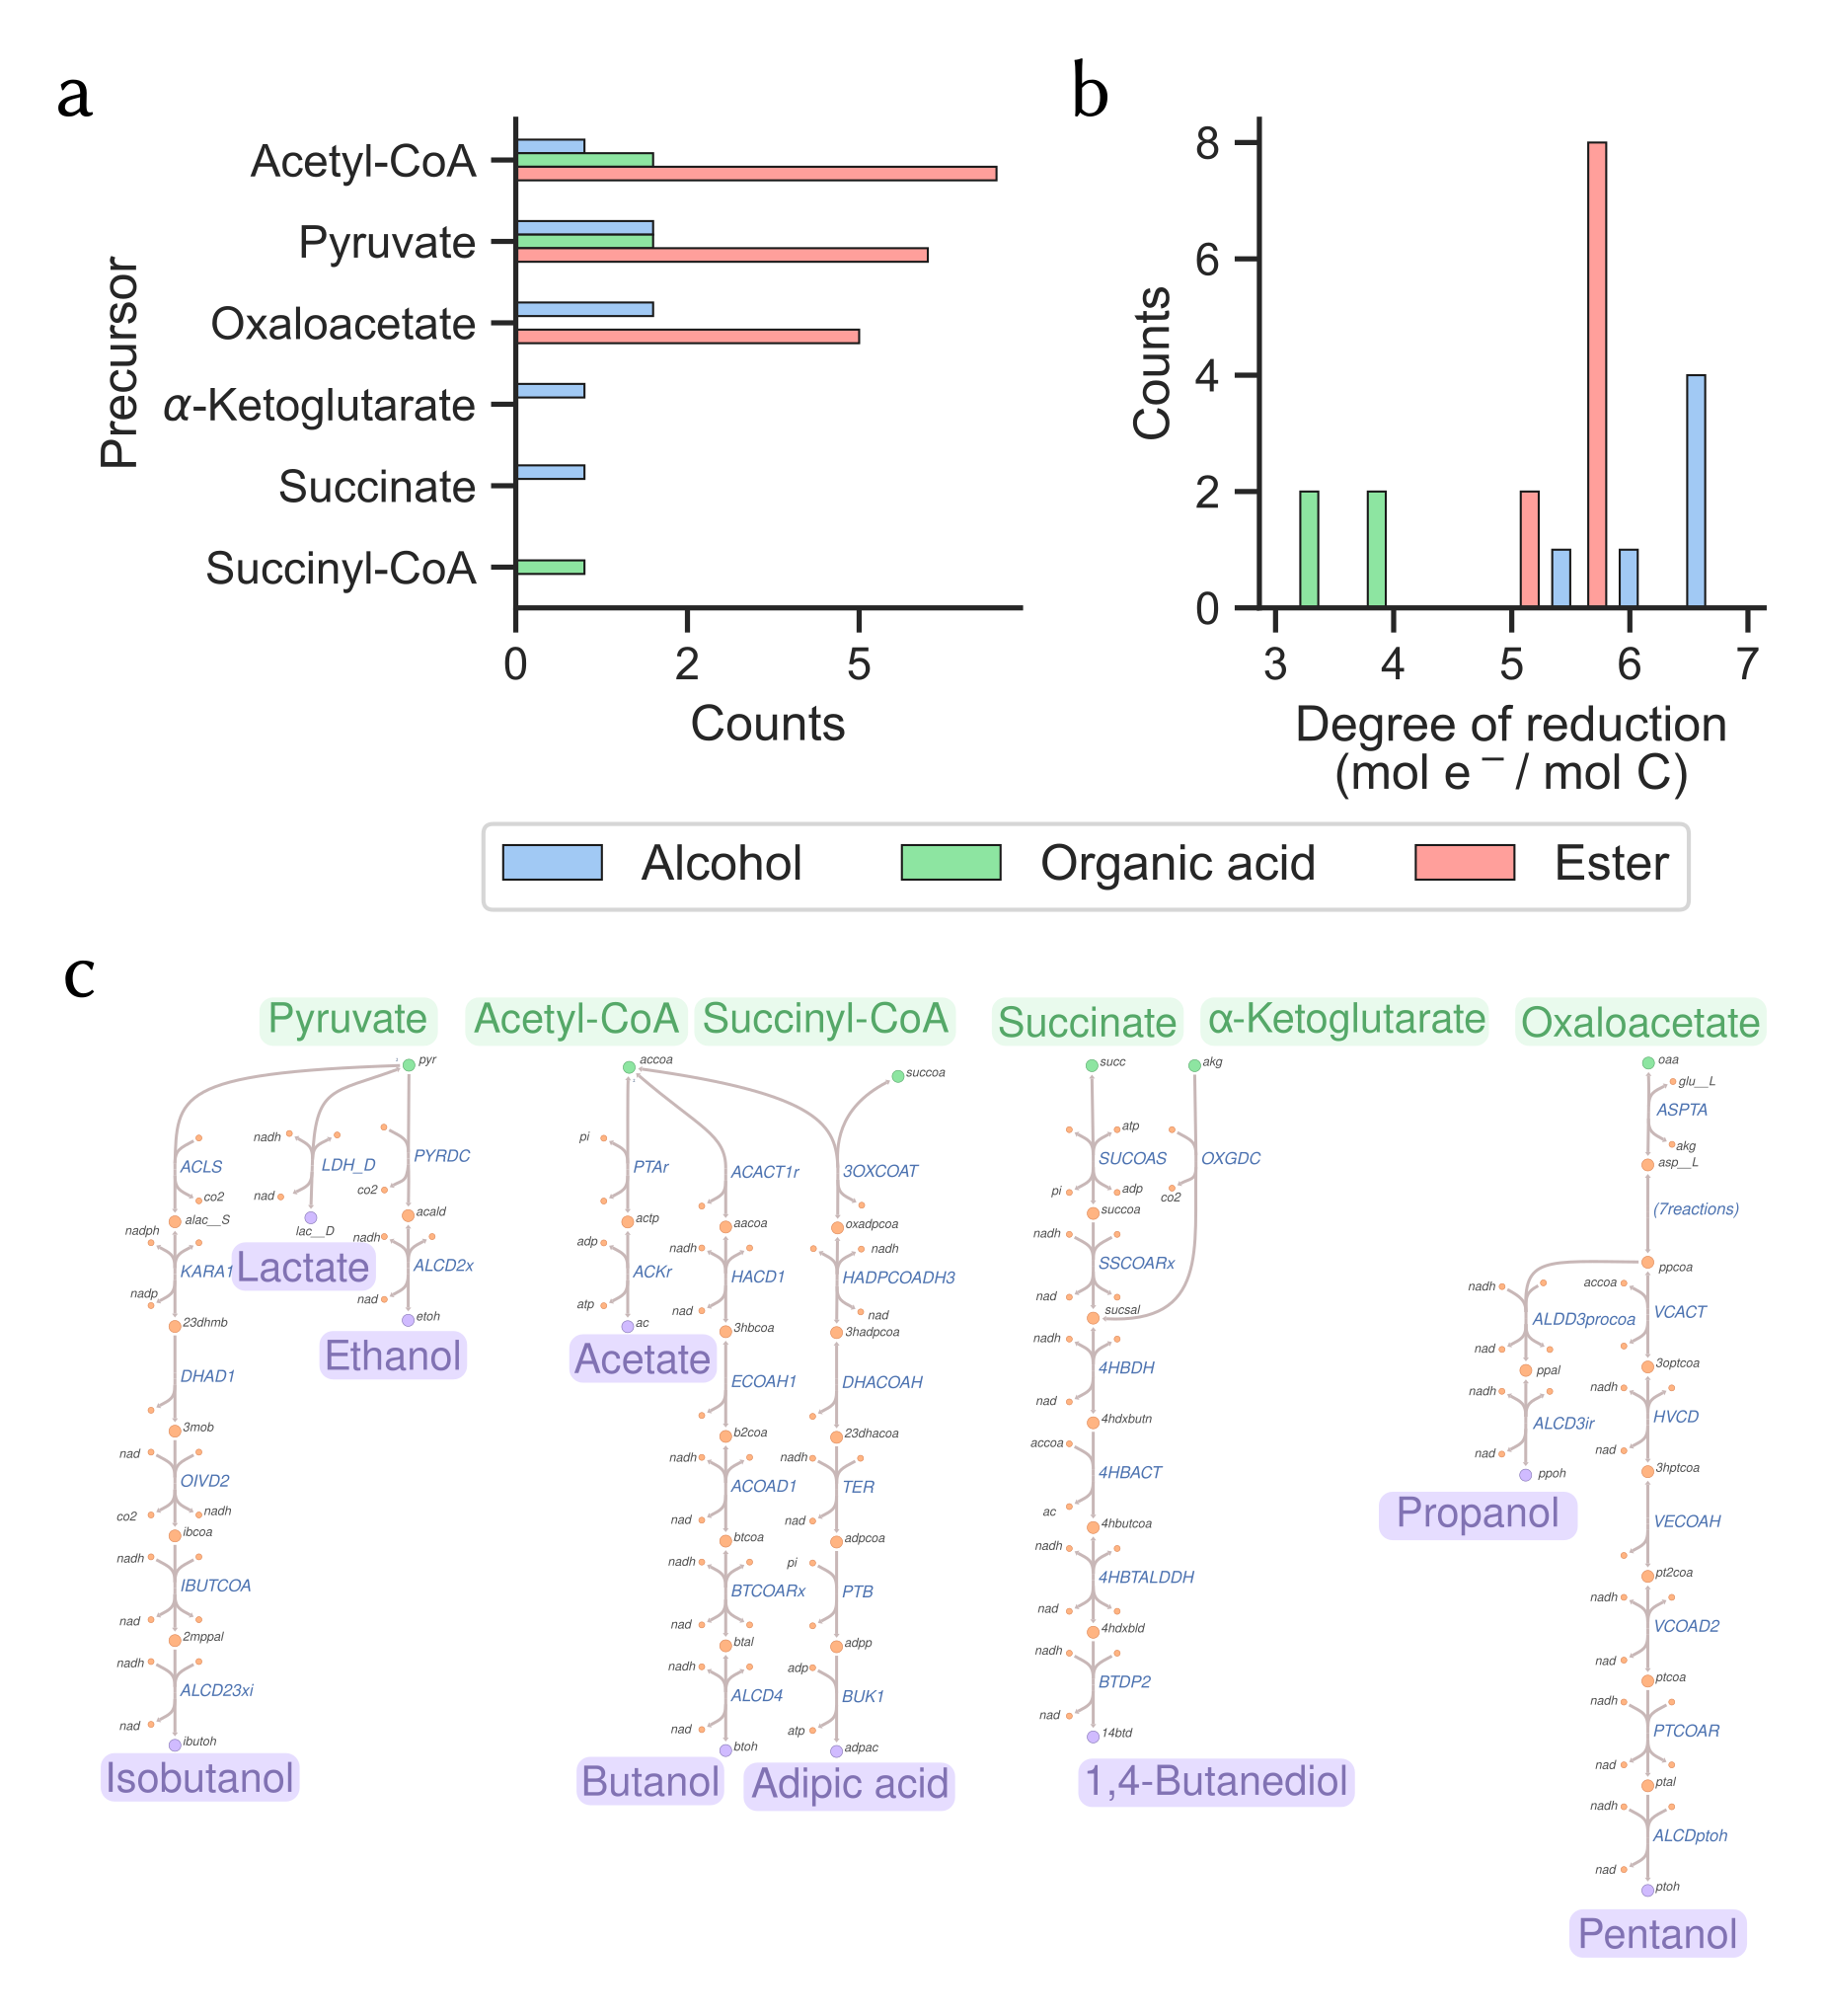
\includegraphics[width=0.7\textwidth,keepaspectratio]{Figure-S1}
    \caption[Biochemical and metabolic diversity of the 20 production modules]{
Biochemical and metabolic diversity of the 20 production modules. (a) Precursor metabolite distribution, using the 12 essential biomass precursors as a reference. (b) Degrees of reduction of the produced metabolites. (c) Production pathway metabolic modules excluding esters.
    }
    \label{fig5:fig-s1}
\end{figure}
%}

\subsubsection{ModCell2-MILP simulations}
ModCell2-MILP was implemented using Pyomo \citep{hart2017}, an algebraic modeling language embedded in the Python programming language. All simulations were performed on a computer with an Intel Core i7-3770 processor, 32 GB of random access memory, and the Arch Linux operative system. The implementation and scripts used to generate the results of this manuscript are available as part of the ModCell2 package via File S2  and \url{https://github.com/trinhlab/modcell2}.
\subsubsection{Optimization solver configuration} \label{sec:solver}
 The Pyomo \citep{hart2017} implementation of ModCell2-MILP was solved with IBM Ilog Cplex 12.8.0. To avoid incorrect solutions associated with numerical issues the following Cplex parameters were changed from their default values: (i) \textit{numerical emphasis} was set to ``true", (ii) \textit{integrality tolerance} was lowered to $10^{-7}$, and (iii) the \textit{MIP pool relative gap} was increased to $10^{-4}$ for enumerating alternative solutions.  Alternative solutions were enumerated using the Cplex ``populate" procedure.


\subsection{Analysis methods}
\subsubsection{Reference flux distribution} \label{sec:flux}
The reference flux distribution, $\frac{v_{jk}^*}{|v_{Sk}^*|}$, is determined by solving the following quadratic program based on the parsimonious enzyme usage hypothesis \citep{machado2014, lewis2010}:
\begin{alignat}{3}
    & \underset{v_{jk}}{\text{min}} \label{eq5:pfba_obj}
\quad \sum_{j \in \mathcal{J}_k} v_{jk}^2 \\
\nonumber & \text{s.t. }  \qquad \\
	& \qquad 	\sum_{j\in \mathcal{J}_k} S_{ijk} v_{jkm} =0  \quad && \forall i\in \mathcal{I}_k 		\label{eq5:pfba_mass_bal}\\
	& \qquad  l_{jk}  \le v_{jk} \le u_{jk} \;  && \forall j\in \mathcal{J}_k 			\label{eq5:pfba_bounds}\\
	& \qquad  v_{Xk} = \text{MaxDesignBio} 			\label{eq5:pfba_bio}
\end{alignat}
\noindent  Constraint \eqref{eq5:pfba_mass_bal} corresponds to mass balance for the metabolic network.
Constraint \eqref{eq5:pfba_bounds} corresponds to reaction bounds, including reaction deletions found in the modular cell design problem.
Constraint \eqref{eq5:pfba_bio} fixes the biomass formation rate, $v_{Xk}$, to the maximum reachable by the design.
This value (MaxDesignBio) is obtained by maximizing $v_{Xk}$ subject to \eqref{eq5:pfba_mass_bal} and \eqref{eq5:pfba_bounds}.
The reference flux distribution $\frac{v_{jk}^*}{|v_{Sk}^*|}$ represents the desired metabolic state of a \textit{wGCP} designed production network. This distribution, if feasible, is unique because the convex optimization problem is formulated with a positive definite quadratic objective function (see Theorem 16.4 in Nocedal and Wright\citep{nocedal2006}). % This is not hard to show here given that the objective function is strictly convex. However, showing the strict convexity requires multivariate calculus (taylors series or frechet derivatives) which are very likely to loose our audience.


\subsubsection{Flux variance clustering}

Flux variance clustering (FVC) seeks to identify and group reactions that exhibit high flux changes under different conditions. Reactions with high flux variance can be considered as metabolic interfaces between core metabolic processes and pathway modules. In our study, each condition corresponds to a different product synthesis phenotype.  FVC implementation entails three steps. First, flux distributions are simulated for each condition and standard deviations for each reaction are calculated. Then, a standard deviation threshold is set to select the reactions with highest flux changes across conditions. Finally, these selected reactions are clustered to identify patterns that repeat under specific conditions. The filtering threshold is set to capture the top reactions with most change while maintaining a sufficiently small list that is biologically meaningful. In our study, we chose an \emph{ad-hoc} value that captures well-known reactions in \textit{E. coli} central metabolism. To cluster the selected reactions, only flux magnitudes, not directionality, were considered in our study. Further, each reaction flux was normalized by the maximum value of that same reaction across all production networks. Clustering was performed using the method \emph{clustermap()} with default clustering-related parameters from the Python library Seaborn 0.9.
%In principle, pathway ontology enrichment or biochemical connectivity of the resulting clusters can potentially be used as metrics to systematically identify a threshold but not explored here.


\subsubsection{Flux sampling} \label{sec:sampling}
To determine an ensemble of flux distributions for a production network, we used the ACHR algorithm \citep{kaufman1998} in the COBRA toolbox \citep{heirendt2017}. Constraints for flux sampling simulation include the reaction deletions and module reactions found in the ModCell design problem solution, a fixed substrate uptake rate of -10 mmol glucose/gCDW/hr, and a minimum product synthesis flux of 50\% of its maximum value.

\subsubsection{Metabolic map drawing}
Drawings of metabolic map were performed using the Escher \citep{king2015a} tool (\url{https://escher.github.io}) that produces \textit{svg} files. Coloring, highlighting candidate reactions, and other systematic adjustments of metabolic maps were done with the Python-based \textit{lxml} module. Additional editing for visual enhancement was done with the Inkscape software.



\section{Results and discussion}

\subsection{Performance and solution time optimization of ModCell2-MILP}
\subsubsection{ModCell2-MILP can not only reproduce the results of the original ModCell2 formulation but also find more alternative solutions}
To evaluate ModCell2-MILP, we compared its performance with the previously developed ModCell2 platform\citep{garcia2019} that solves the optimization problem with multi-objective evolutionary algorithms (MOEAs). As a basis of comparison, we used the same \textit{E. coli} core metabolic model, maximum number of deletion reactions $\alpha$, and maximum number of module-specific reactions $\beta_k$ for both ModCell2 and ModCell2-MILP. Due to fundamental differences in problem formulations for MOEA and MILP, we used the \textit{lsGCP} design objective for ModCell2-MILP with multiple weighting factors, $a_k$, specifically selected to reproduce previous results, in the blended formulation and the \textit{sGCP} design objective for ModCell2 (File S1). The results showed that ModCell2-MILP could generate the same Pareto optimal designs like ModCell2. In addition, ModCell2-MILP enumerated a larger number of alternative solutions than ModCell2. For example, the design named \textit{sGCP-5-0-6} generated by ModCell2 had 3 alternative solutions while ModCell2-MILP found 8 alternative solutions. By increasing $\alpha$ to 8 and $\beta$ to 2, we could identify a utopia design (i.e., one solution with the maximum value for all objectives) with 192 alternative solutions, expanding the possibilities for experimental implementation.


\subsubsection{Tuning MILP formulations significantly improves solution times}
We considered three techniques that can improve solution times of ModCell2-MILP, including:

(i) \textit{Fixing the network feasibility indicator} $w_k$. If all modules are expected to be compatible with a final ModCell design (i.e., $f_k > 0,\, \forall k \in \mathcal{K}$), $w_k$ is set to be 1 for all $k \in \mathcal{K}$ to avoid computational efforts in finding non-optimal feasible solutions.

(ii) \textit{Flux bound tightening}. Constraints of the form $ e_{jkm} l_{jkm} \le v_{jkm} \le e_{jkm} u_{jkm}$ are known to result in weak linear relaxations, i.e., feasible values of $v_{jkm}$ are far from their bounds $l_{jkm}$ and $u_{jkm}$. To tighten the formulation by making continuous relaxations closer to the feasible integer solution, smaller values of $u_{jkm}$ and $l_{jkm}$ are determined by solving a series of linear programs that maximize and minimize each flux $v_{jkm}$ in the parent production networks $\Pi_{km}(e_{jk}=1, \, \forall j \in \mathcal{J}_k)$.

(iii) \textit{Benders decomposition}. ModCell2-MILP has a separable structure compatible with Benders decomposition\citep{geoffrion1972, fischetti2016} that creates a  master problem, using binary variables and associated constraints \eqref{eq5:acon}-\eqref{eq5:w_symmetry}, and sub-problems for each production network $\Psi_{km}(e_{jk})$ with fixed binary variables. This decomposition implementation is automatically done by Cplex 12.8.

We evaluated these three techniques for tuning MILP formulations and used the core\textit{ E. coli} model\citep{garcia2019} for the benchmark study. The results showed that flux bound tightening, fixed $w_k$, and Benders decomposition could reduce the solution time to find solutions by 50\%, 80\%, and  95\%, respectively (Table~\ref{tab5:timing}). By combining these techniques, the solution time was shortened by 96\% from 63.3 s to 2.8 s. In subsequent studies, we used these three tuning techniques to solve the ModCell design problem unless otherwise noted.

%\begin{table}[!ht]
\begin{table}[ht]
    \caption[Solution time reduction by tuning the ModCell2-MILP formulation]{Solution time reduction by tuning the ModCell2-MILP formulation.
    Fixed network indicator means $w_k = 1\;, \forall k \in \mathcal{K}$. The simulations were performed in triplicates.
    }
    \centering
	%Table: Solution times (n=3) for \alpha=5 and \beta=1 and objective lsGCP.
\rowcolors{2}{gray!25}{white}
\begin{tabular}{cccc}    \toprule
	\multicolumn{1}{>{\centering\arraybackslash}m{20mm}}{Feasibility indicator $w_k$  fixed} &
	\multicolumn{1}{>{\centering\arraybackslash}m{20mm}}{Benders decomposition} &
	\multicolumn{1}{>{\centering\arraybackslash}m{20mm}}{Bounds tightened} &
	\multicolumn{1}{>{\centering\arraybackslash}m{20mm}}{Solution time (s)} \\
	\midrule
	No&No&No&63.3 $\pm$ 16.9 \\
	No&No&Yes&32.5 $\pm$ 10.2 \\
	No&Yes&No&3.6 $\pm$ 0.1 \\
	No&Yes&Yes&3.4 $\pm$ 0.4 \\
	Yes&No&No&13.8 $\pm$ 2.7 \\
	Yes&No&Yes&11.9 $\pm$ 1.7 \\
	Yes&Yes&No&2.7 $\pm$ 0.3 \\
	Yes&Yes&Yes&2.8 $\pm$ 0.1 \\
 \hline
\end{tabular}



    \label{tab5:timing}
\end{table}

\subsubsection{Choice of design parameters affect solution time}
In designing a modular cell with ModCell2-MILP, the designer needs to specify the formulation type (i.e., blended or goal attainment formulation), the target phenotype (e.g., \textit{wGCP, lsGCP}, and \textit{NGP}), and the limits of deletion reactions ($\alpha$) and endogenous module-specific reactions ($\beta_{k}$). We evaluated the impact of these parameters on solution time using the \textit{E. coli} core model (Figure~\ref{fig5:times}).  Regardless of the formulation type, increasing $\alpha$ and $\beta$ led to harder problems and hence required more solution time due to the exponentially increasing number of feasible solutions as expected. The goal attainment formulation took longer time to solve for the \textit{lsGCP} and \textit{NGP} design objectives, but about the same time for the \textit{wGCP} design objective. Interestingly, the overall difficulty of \textit{wGCP} is higher than that of \textit{lsGCP} in both the blended and goal attainment formulations, despite \textit{lsGCP} having approximately twice the number of constraints. Furthermore, the \textit{NGP} design objective could be solved most quickly, likely due to the narrower design space associated with the no-growth associated production of target metabolites.

%\afterpage{%
\begin{figure}[hp]
    \centering
    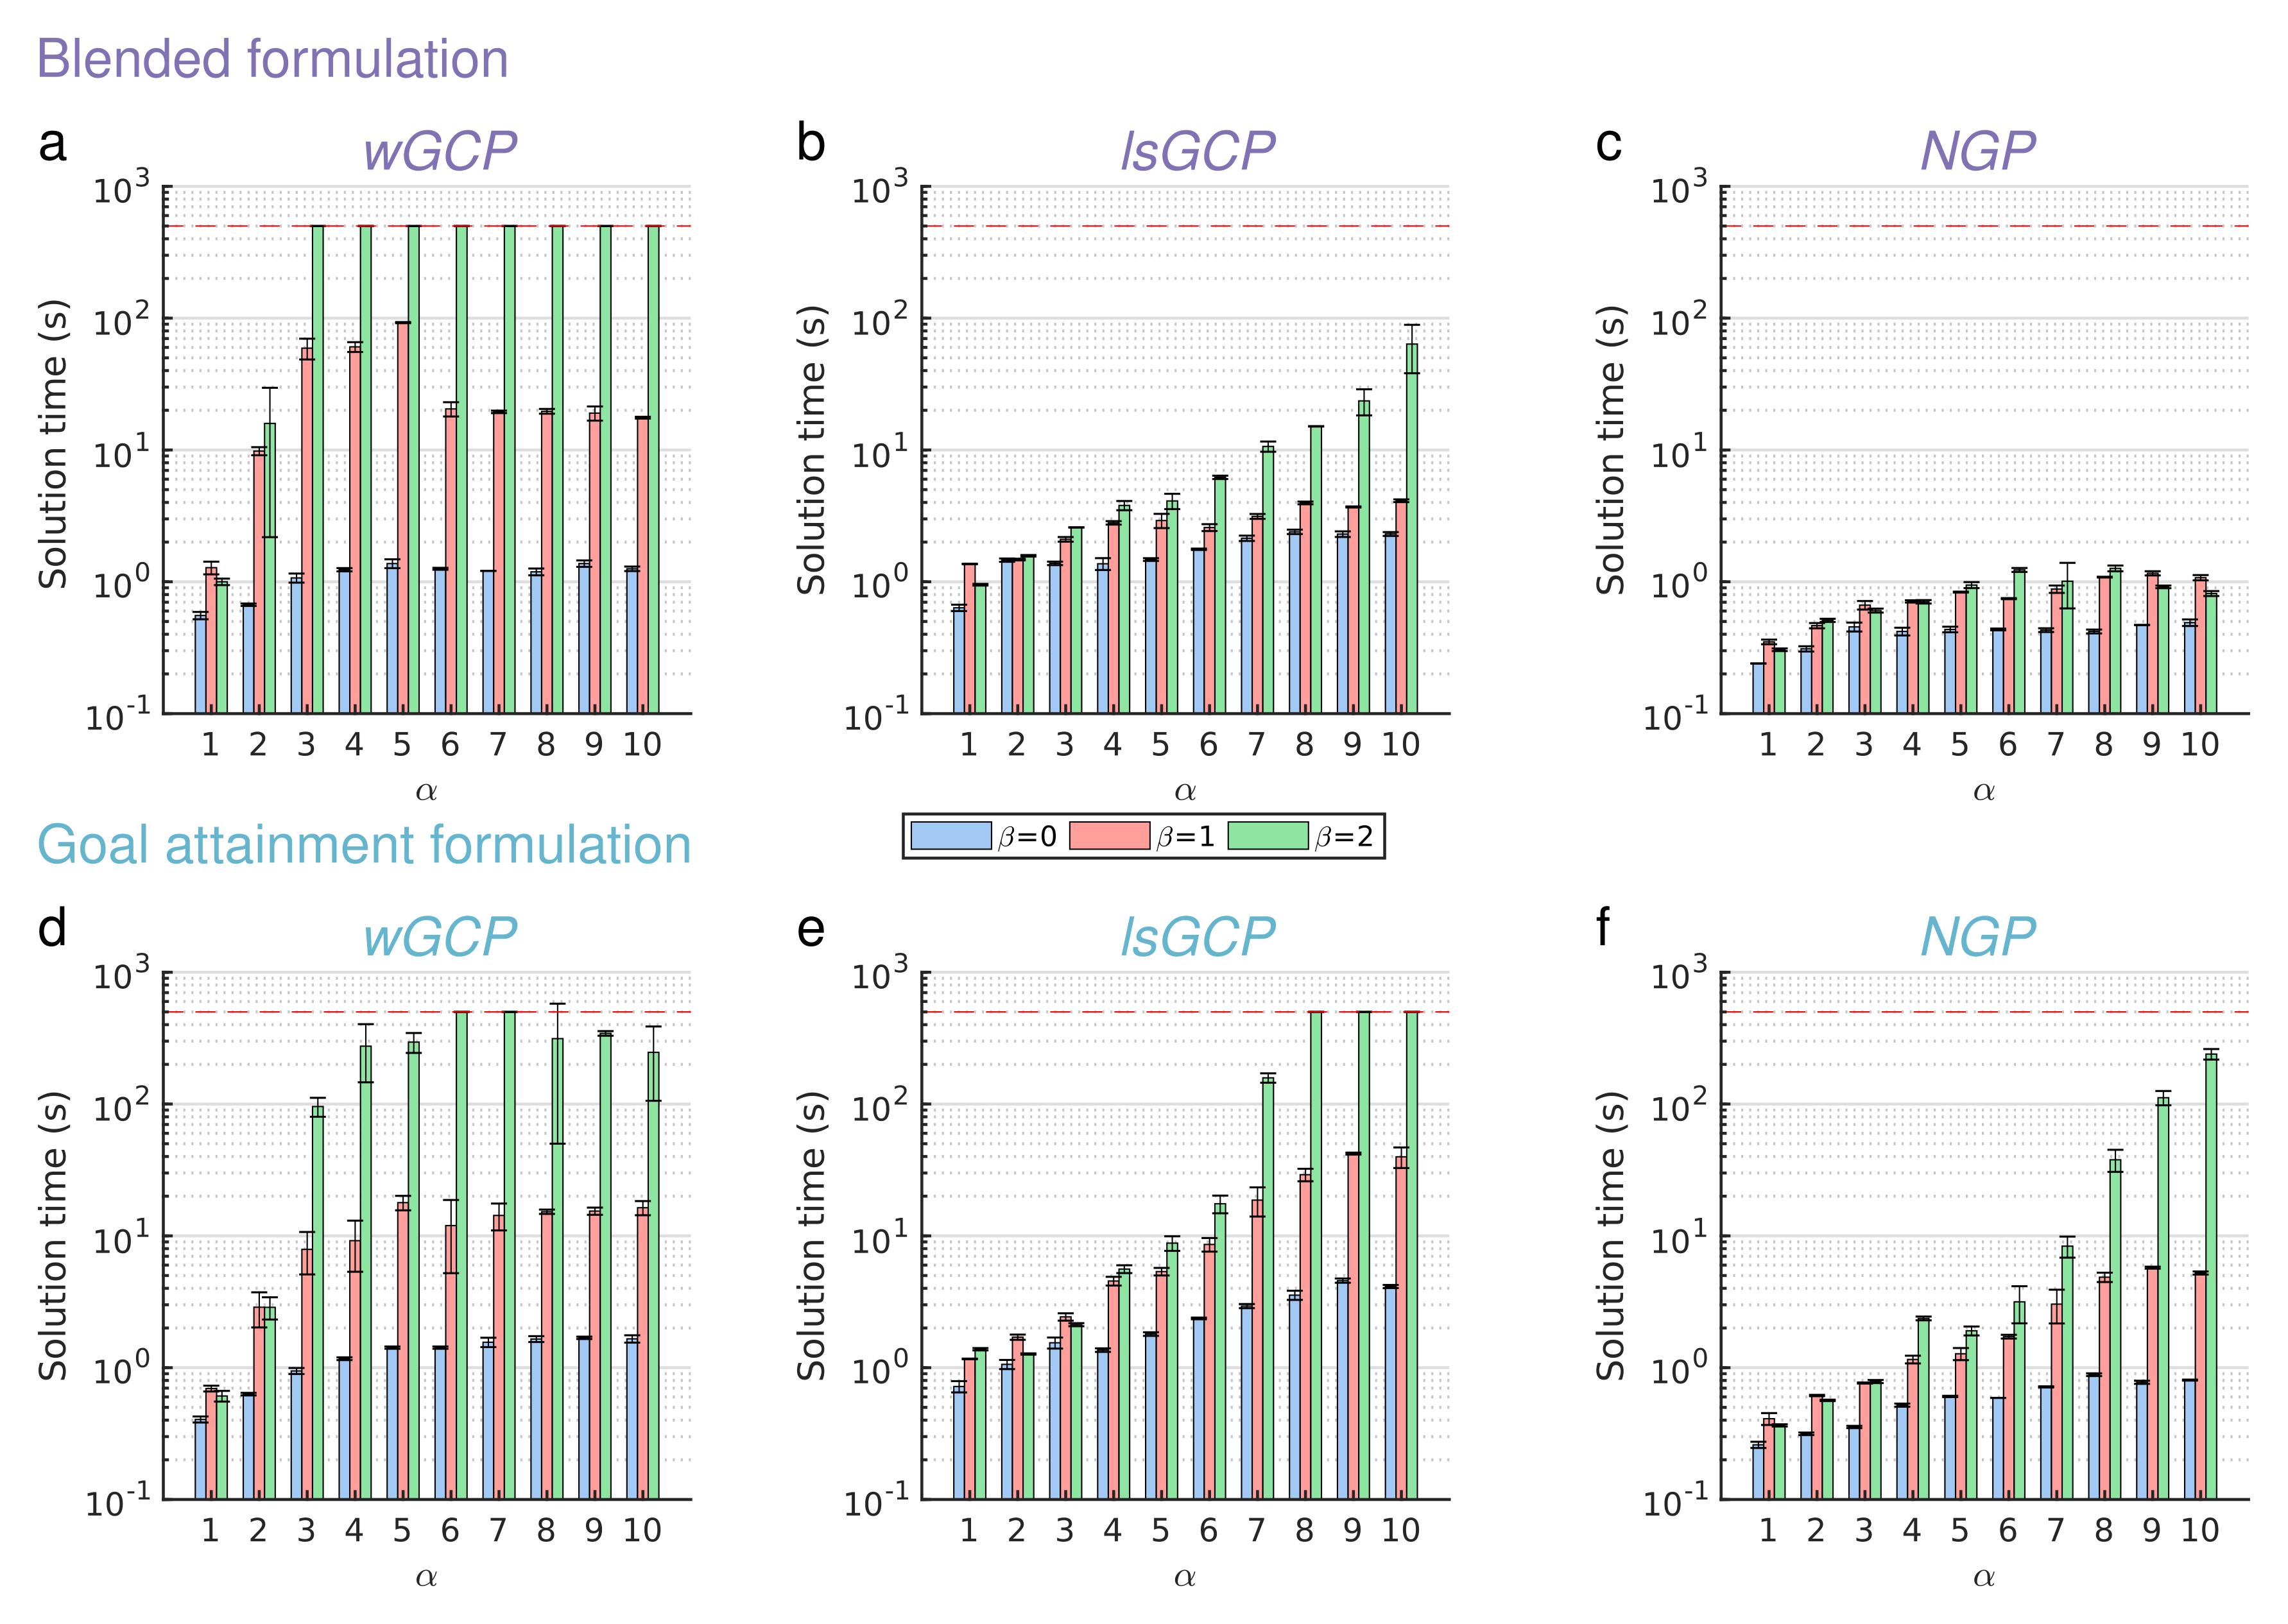
\includegraphics[width=\textwidth,height=\textheight,keepaspectratio]{performance-timing.png}
    \caption[Effect of design parameters on solution time]{Effect of design parameters on solution time. We examined the target design objective (i.e., \textit{wGCP}, \textit{lsGCP}, and \textit{NGP}) and the limits of deletion reactions $\alpha$ and endogenous module-specific reactions $\beta_k$, on computation time for solving the ModCell2-MILP problem with the blended (a-c) and goal attainment (d-f) formulations. A time limit of 500 seconds indicated by a red dashed line was used in all cases, but only reached by certain \textit{wGCP} and \textit{lsGCP} cases with $\beta \ge2$. The simulations were performed in duplicates.}
    \label{fig5:times}
\end{figure}
%}

\subsection{Design of a universal modular cell for a genome-scale metabolic model of \textit{E. coli}} \label{sec:univ_design}

\subsubsection{Reduction of the candidate reaction deletion set enables ModCell2-MILP to find modular cell designs for a large-scale metabolic network}

Finding genetic modifications towards a desired phenotype using mathematical optimization for large-scale metabolic networks is a computationally expensive task, due to the combinatorial search space spanned by a large number of reaction deletion candidates in the network \citep{feist2010, kamp2014}.
Preprocessing of metabolic networks to reduce reaction candidates is not only critical but also practical for experimental implementation. The set of reaction candidates in the iML1515 \textit{E. coli} model\citep{monk2017} was reduced from 2,712 to 276 by ModCell2 \citep{garcia2019}. Using this model and the \textit{wGCP} objective, an \textit{E.~coli} modular cell was then identified to be compatible with 17 out of 20 products with requirement of only 4 reaction deletions \citep{garcia2019}.
Since MOEA implemented in ModCell2 does not guarantee optimality, here we aimed to evaluate the capability of ModCell2-MILP for handling a large-scale metabolic network and identifying the Pareto optimality and potential alternative solutions.

We applied ModCell2-MILP to analyze the same iML1515 model with a set of 20 products using the same design parameters (i.e., $\alpha$ and $\beta_k$) and the blended formulation with all objective weights $a_k=1$. The simulation shows that ModCell2-MILP could not solve the ModCell design problem to optimality over 2 days of run time, likely due to the large number of candidate deletion reactions still present in the genome-scale model. Currently the best MILP solution algorithms do not scale well with parallel computing. In order to obtain solutions within an acceptable time, the set of candidate reactions must be further reduced. Since only a small subset of all metabolic reactions in genome-scale models tend to be deleted by strain design algorithms \citep{feist2010, king2017, garcia2019}, we used a pool of \textit{wGCP} designs with $\alpha= 4,5,6$ and $\beta = 0,1$ reported with ModCell2 \citep{garcia2019} to identify relevant deletion candidates. From a set of 601 designs found by ModCell2, only 33 out of 276 reaction deletion candidates were used at least once. Hence, these 33 reactions were used to create a new, computationally-tractable set of reaction candidates. This new set contains reactions mostly from the well-characterized central metabolic pathways (Figure~\ref{fig5:candidate-reactions}a) while the original set includes reactions in peripheral pathways that lead to biomass synthesis. Interestingly, within these 33 reaction candidates, only a few are used in most designs (Figure~\ref{fig5:candidate-reactions}b), highlighting the importance of their removal in growth-coupled production phenotypes. Reactions with high deletion frequencies mainly occur in high-flux central metabolic pathways (Figure~\ref{fig5:candidate-reactions}c), closely associated with cellular energetics and carbon precursors that interface with the production modules (Figure~\ref{fig5:candidate-reactions}d).

\begin{figure}[p]
    %\textit{Figure on previous page.}}
    \centering
    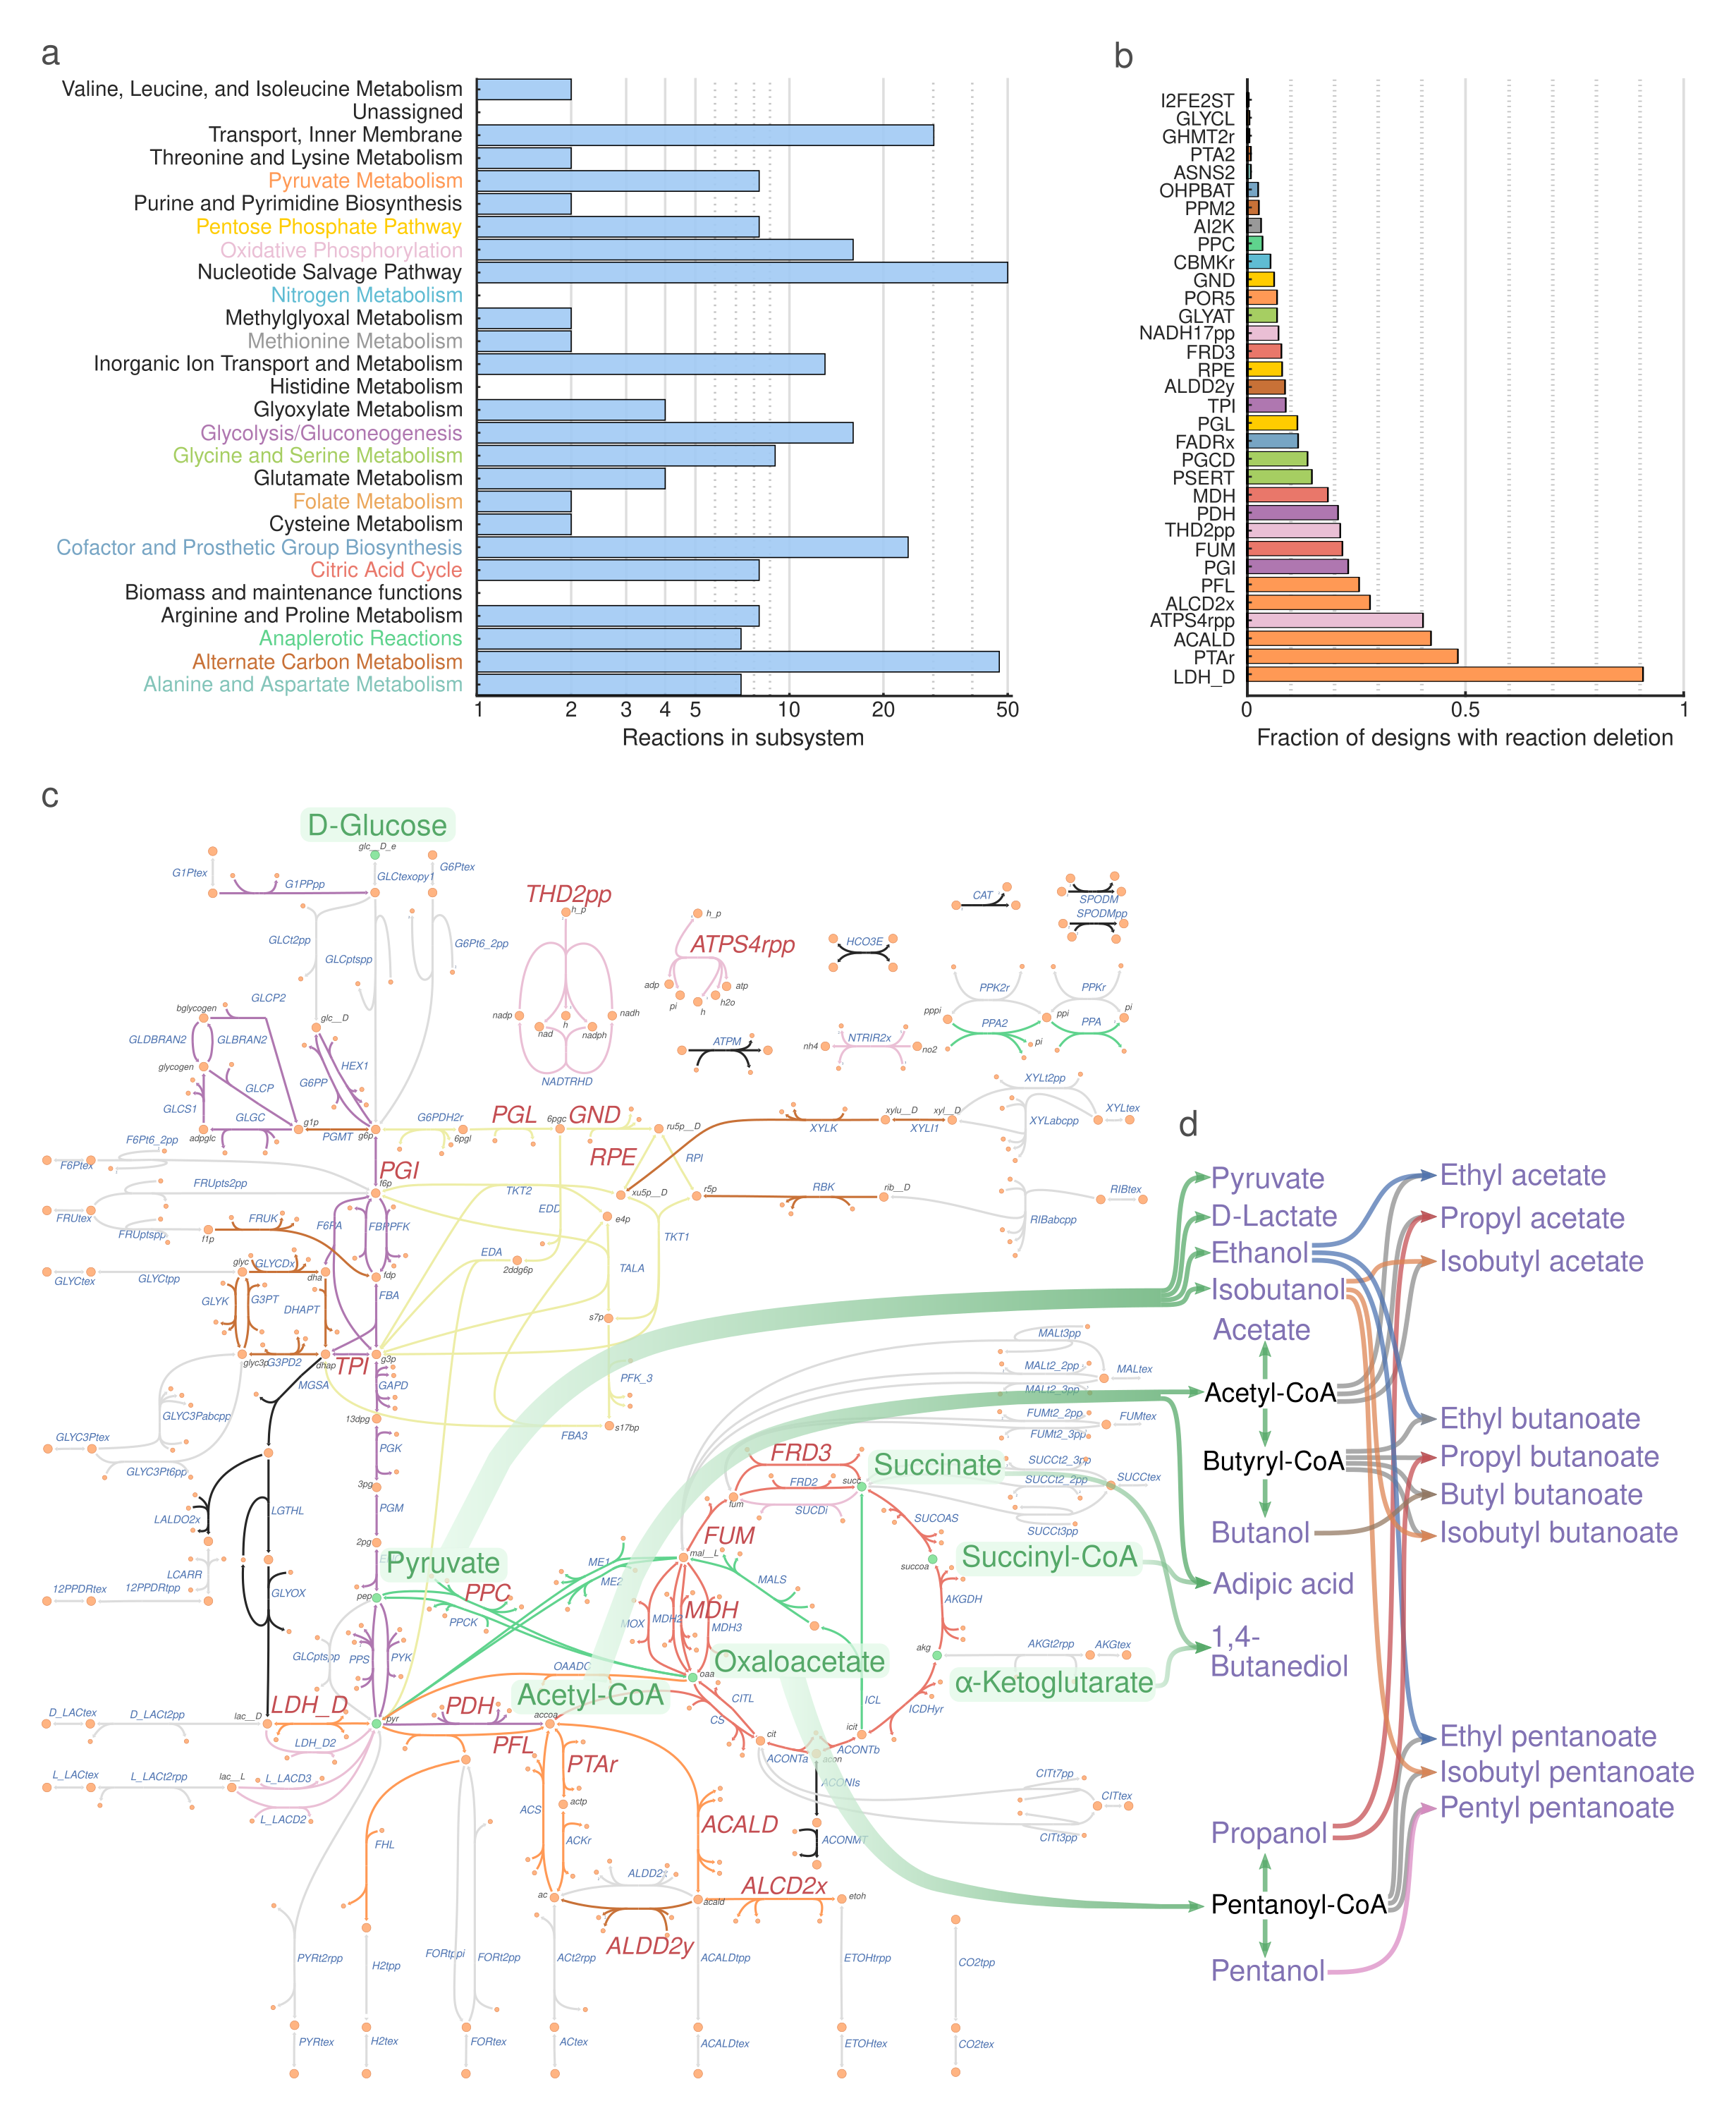
\includegraphics[height=.71\textheight,keepaspectratio]{candidate-reactions.png}
    \caption[Metabolic functions of deletion candidate reactions]{Metabolic functions of deletion candidate reactions. (a) Subsystem distribution for the original set of 276 candidate reactions in the iML1515 model. Those subsystems that contain a reaction used in at least one design are colored.  (b) Deletion frequency for the reduced set of 33 candidate reactions. The analysis is based on a pool of 601 \textit{wGCP} designs from different $\alpha$ and $\beta$ parameters whose Pareto fronts were previously determined with ModCell2.\citep{garcia2019} Bar colors indicate membership of these reactions to the subsystems. (c) Metabolic map of core metabolism. Key metabolites, including precursors for the 20 product modules (i.e., pyruvate, acetyl-CoA, succinyl-CoA, succinate, and $\alpha$-ketoglutarate), are highlighted in green. Reactions are colored according to subsytem labels indicated in (a), reactions colored in light gray do not appear  in any of the subsytems of (a), and reactions that are candidates for deletion, listed in (b), are labeled in red. (d) Link between major precursors and target products where colors are only used to facilitate visualization. Reaction and metabolite abbreviations correspond to BiGG\citep{king2015} identifiers (\protect\url{http://bigg.ucsd.edu/}).
    }
    \label{fig5:candidate-reactions}
\end{figure}
%\addtocounter{figure}{-1}
%\afterpage{%
%\begin{figure}[H]
    %\caption{\textit{Caption on next page.}}
	%\centering
    %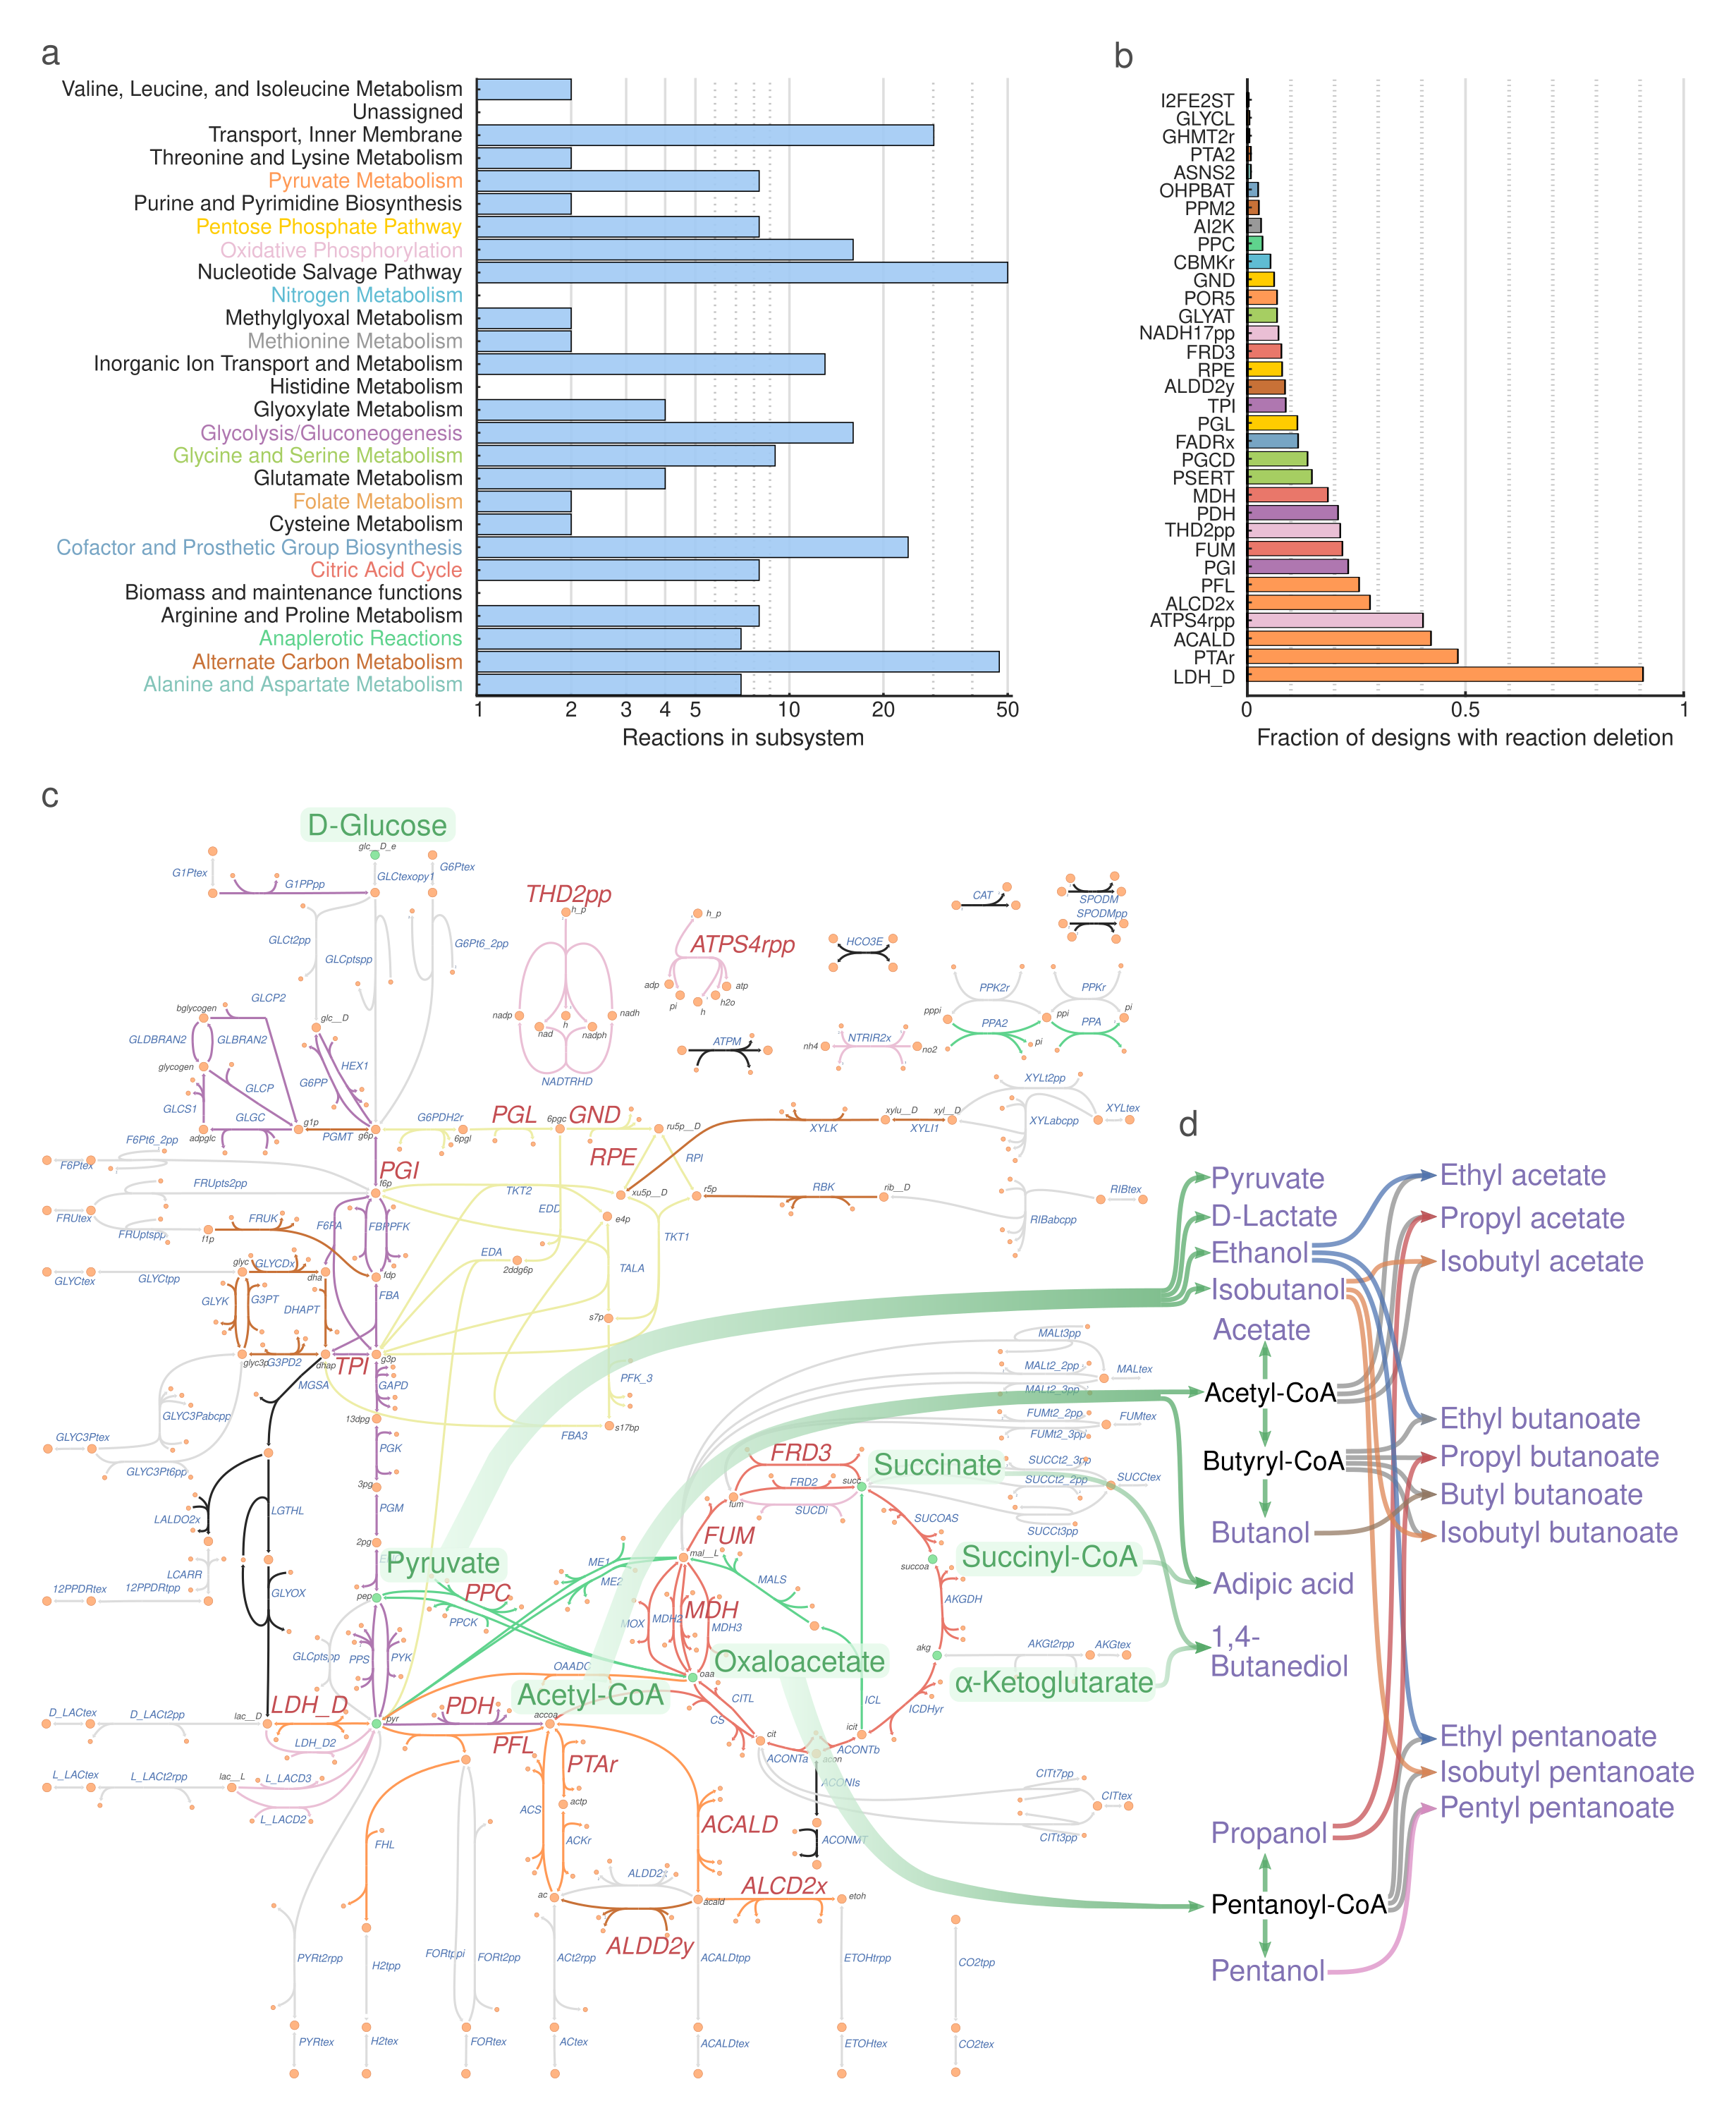
\includegraphics[height=\textheight,keepaspectratio]{candidate-reactions.png}
%\end{figure}}

Using the reduced reaction deletion candidate set, ModCell2-MILP could find an optimal solution in $\sim 30$ min and enumerated all optimal solutions in $\sim 8$ hours. All the optimal solutions found by ModCell2-MILP in this case were in agreement with those previously found by ModCell2 \citep{garcia2019}. It should be noted that a reduced deletion candidate set can be identified for any metabolic model and target products by using previous designs identified with either ModCell2 or single-phenotype strain design algorithms \citep{long2015}. This heuristic for reaction deletion candidate selection might affect design optimality to the extent that it omits relevant reactions. However, using a sufficiently informative pool of designs from other strain design algorithms helps minimize the chances of missing relevant candidates.


\subsubsection{ModCell2-MILP can identify a universal modular cell compatible with all exchangeable production modules} \label{sec:universal_design}
Based on the computationally tractable reaction deletion candidate set, we next evaluated whether the goal programming formulation could help identify a universal ModCell design that is compatible with all modules.
By screening for increasing $\alpha$ and $\beta_k$, we found that a design with $\alpha=6$ and $\beta_k=1$ could overcome the performance trade-offs between modules and hence constitute a universal modular cell that is compatible with all production networks considered (Figure~\ref{fig5:universal-design}a). Once coupled with a module, each resulting production strain displays the engineered phenotype with the defined minimum objective goal of 0.5 (i.e., 50\% of the theoretical maximum product yield attained at the maximum growth rate).
Remarkably, most products surpassed this minimum goal with yields above 90\% of the theoretical maximum values (Figure~\ref{fig5:universal-design}b). All production networks displayed a feasible metabolic space where an increase in product synthesis rate is needed to attain faster growth rates (Figure~\ref{fig5:universal-design}c). This designed phenotype is useful for optimal pathway selection using adaptive laboratory evolution \citep{fong2005, trinh2009b} and/or pathway libraries \citep{garst2017}.

%\afterpage{%
\begin{figure}[p]
%\begin{adjustwidth}{-2.25in}{0in}
    \centering
    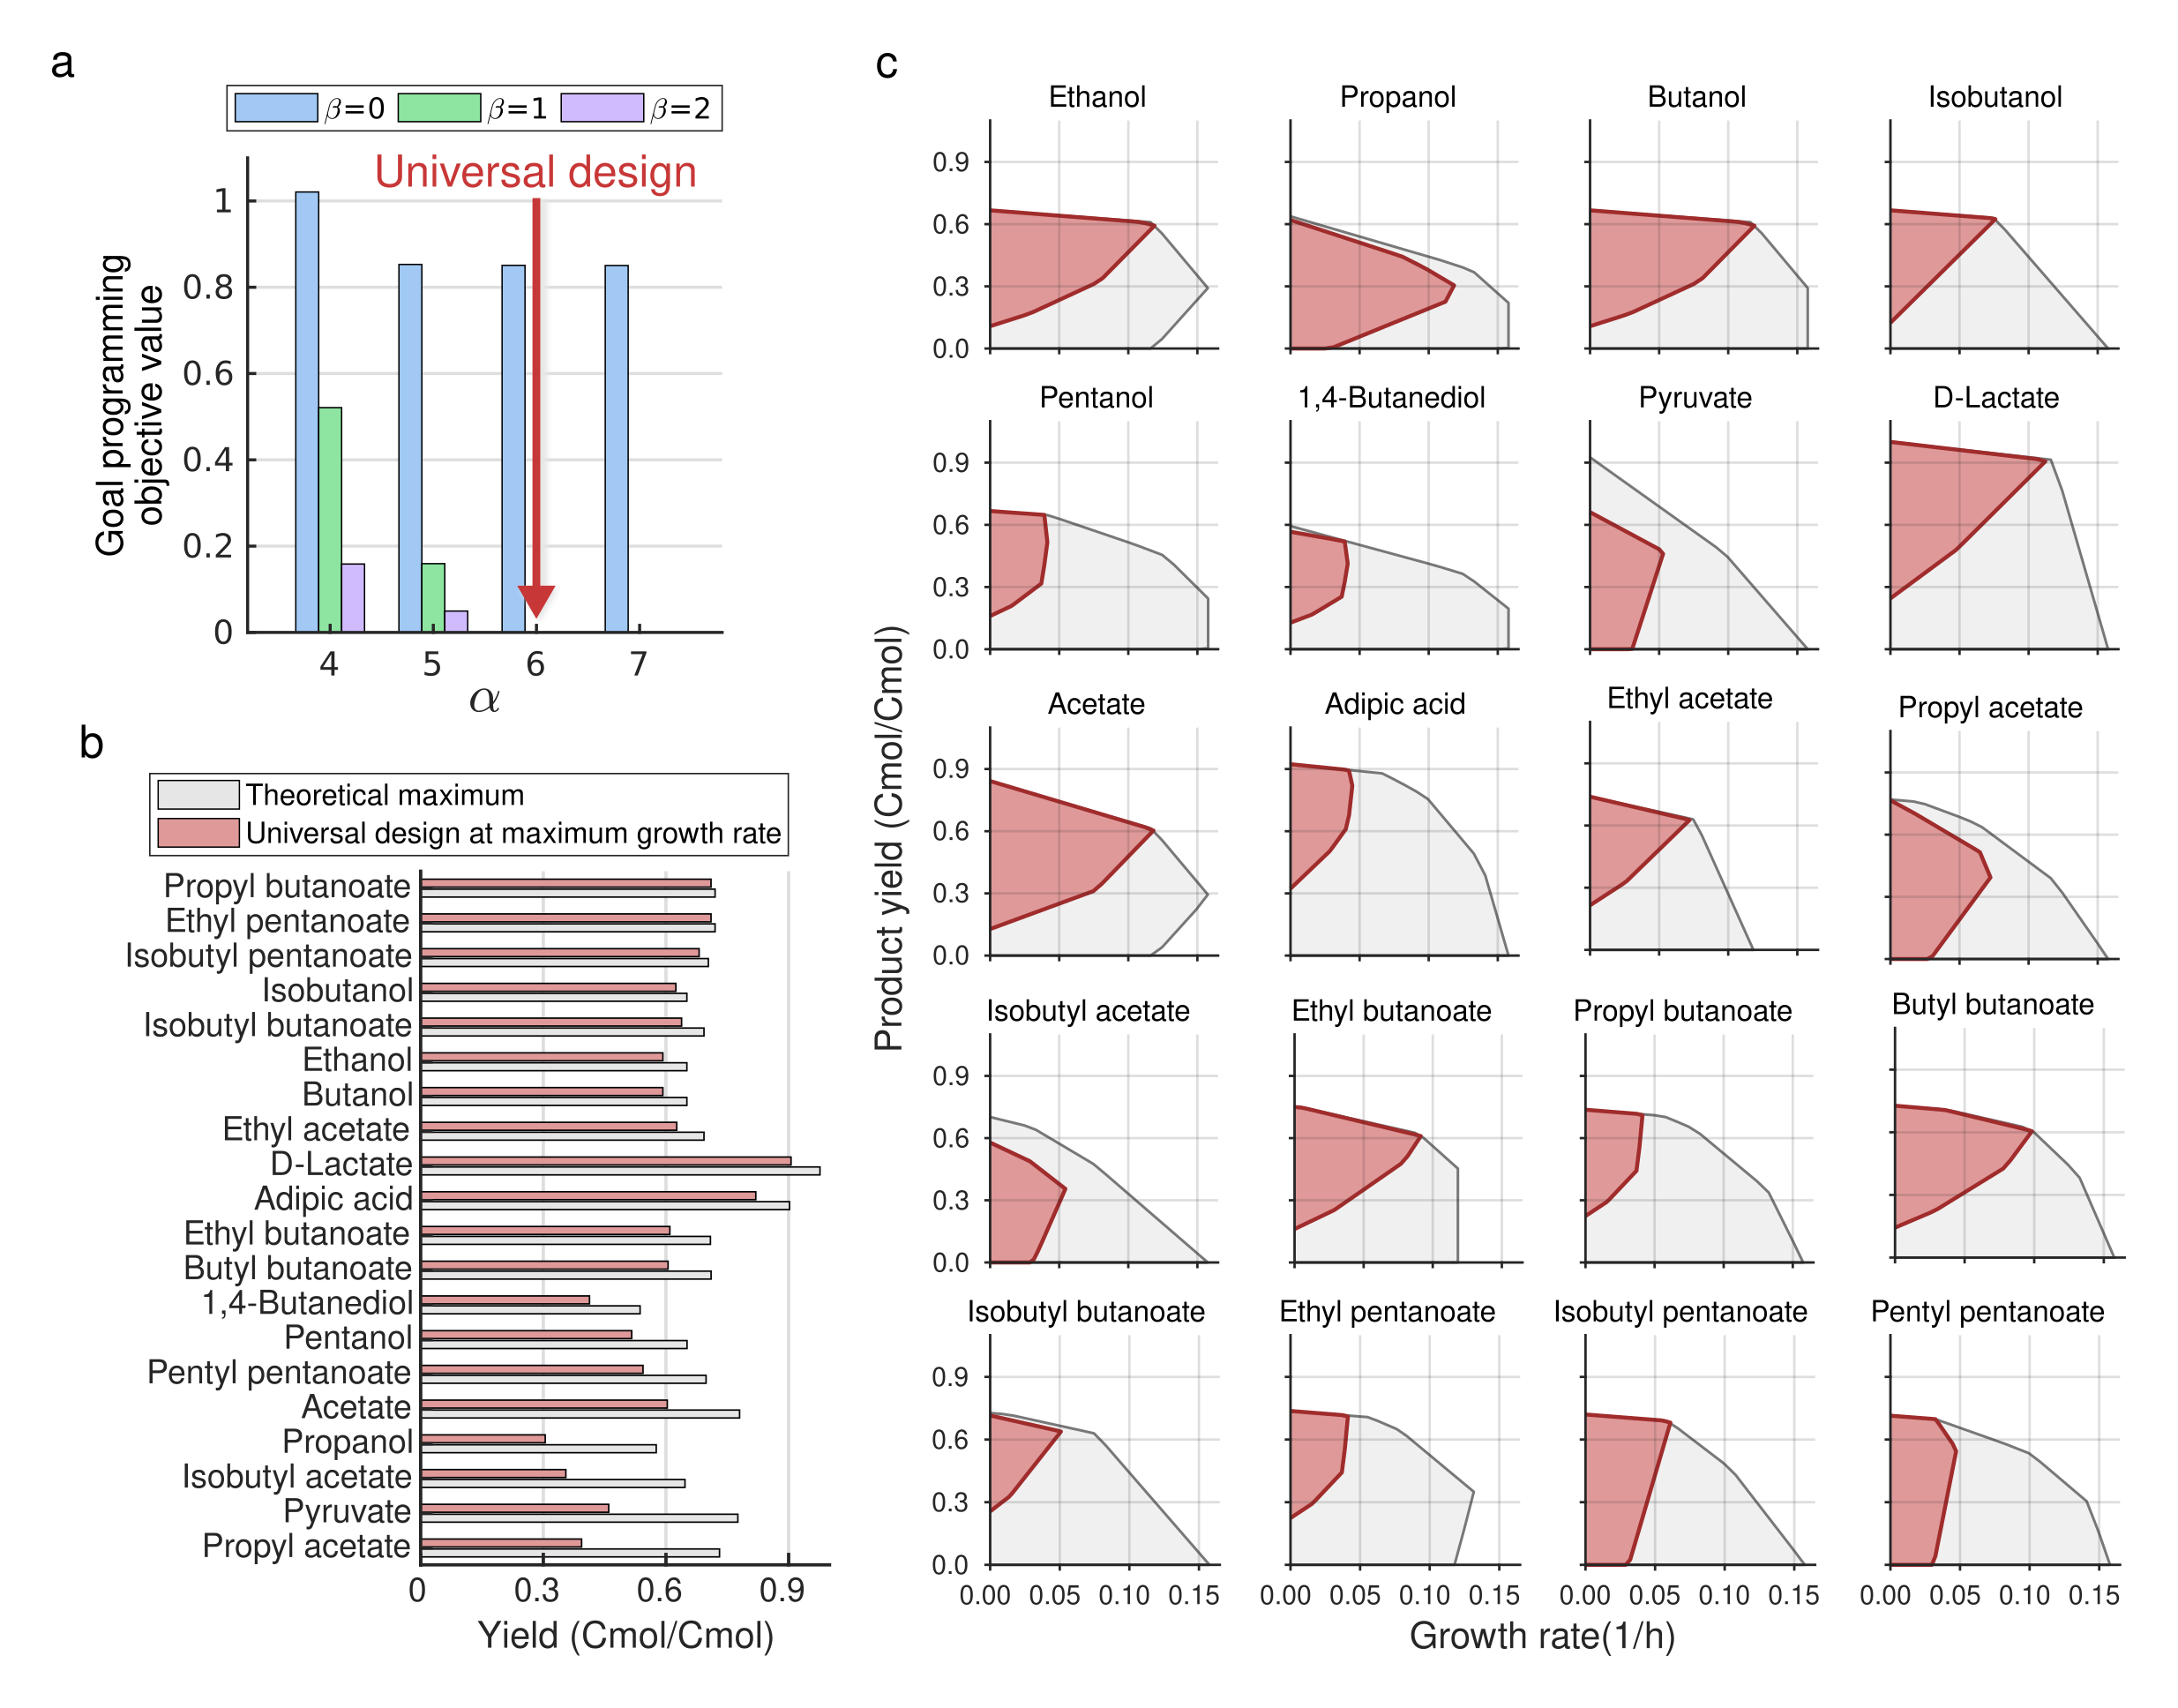
\includegraphics[width=\textwidth,keepaspectratio]{universal-design.png}
    \caption[Identification of a universal modular cell compatible with all production modules under the \textit{wGCP} design phenotype]{Identification of a universal modular cell compatible with all production modules under the \textit{wGCP} design phenotype. (a) Goal programming solutions with increasing $\alpha$ and $\beta$ values. The goal programming objective value \eqref{eq5:goal_obj} in the y-axis measures the difference between the performance of production strains and the target goal, i.e., $\sum_{k\in \{ k \in \mathcal{K}: f'_k < g_k\}}(f'_k - g_k)$ where the target goal is set to be $g_k=0.5$. The parameters $\alpha=6$ and $\beta=1$ are sufficient to identify a universal modular cell design meeting the required goal for all production networks. (b) Comparison between the yield performances of the designed modular production strains and maximum theoretical values. (c) The feasible flux spaces for the wild-type (gray) and designed modular production strains (crimson). Based on the \textit{wGCP} design phenotype, to increase growth rate, each mutant must increase product synthesis rate. The genetic manipulations of this universal modular cell design are indicated in the metabolic map of Figure~\ref{fig5:core-modules}c.}
    \label{fig5:universal-design}
%\end{adjustwidth}
\end{figure}
%}

\subsection{Flexible metabolic flux capacity of \textit{E. coli} core metabolism enables the design of a universal modular cell}

\subsubsection{Endogenous modules responsible for metabolic flexibility of a universal modular cell are identified by comparing flux distributions of production networks}
The designed universal modular cell (Figure~\ref{fig5:universal-design}) can theoretically adapt to the conflicting metabolic requirements of all production modules (Table~\ref{tab5:pathways}).
To gain further insight into this unique metabolic capability of the modular cell, we analyzed the simulated \emph{reference flux distributions} of each production network using the \emph{flux variance clustering} (FVC) analysis (Materials and Methods).
Reactions with the highest flux changes across the production networks are likely critical for the proper operation of the universal modular cell and might present potential bottlenecks.
Such reactions were identified by filtering their reference flux standard deviation calculated across production networks with an \textit{ad hoc} threshold of 0.2 (mol/substrate mol).
Over 90\% of the 535 active reactions, each of which carries a non-zero flux in at least one production network, had standard deviation values below the threshold, indicating  highly conserved metabolic core pathways among production networks. Only 9.5\% of the active reactions presented a standard deviation magnitude above the threshold (Figure~\ref{fig5:core-modules}a).


\begin{table}[ht]
%\begin{table}[!ht]
%\begin{adjustwidth}{-2.25in}{0in}
    \caption[Overall production module pathway stoichiometries and associated simulated secretion fluxes of the universal modular cell design]{Overall production module pathway stoichiometries and associated simulated secretion fluxes of the universal modular cell design.
    DoR is the degree of reduction of the final product (mol~$e^-$ / mol~C). Metabolite secretion profiles are determined from the simulated reference flux distributions (mol~C / mol~C) of the universal modular cell design.
    Flux abbreviations: $r_{p}$, product; $r_{ac}$, acetate; $r_{co_2}$, CO$_2$; $r_{for}$, formate; $r_{succ}$, succinate.
    Note that the negative CO$_2$ fluxes in pyruvate and acetate production networks indicate overall CO$_2$ uptake enabled by phosphoenolpyruvate carboxylase (PPC).}
    \centering
 	%Table : Production networks overall reactions and secreted product yields for the reference flux distributions of the universal design.

\rowcolors{2}{gray!25}{white}
\resizebox{\textwidth}{!}{\begin{tabular}{lcccccc}
\toprule
    Overall reaction  & DoR  & $r_{p}$ & $r_{ac}$ & $r_{co_2}$ & $r_{for}$ & $r_{succ}$ \\
\midrule
pyr + nadh $\rightarrow$ \textbf{ethanol} $|$  accoa + 2 nadh $\rightarrow$  \textbf{ethanol} (native) 		&7.0&0.58&0.01&0.27&0.04&- \\
oaa + glu  + 2 atp + 2 nadph  +  nadh $\rightarrow$ akg + \textbf{propanol}					&6.7&0.31&0.36&0.07&0.18&- \\
2 accoa + 4 nadh $\rightarrow$ \textbf{butanol}									&6.5&0.59&0.01&0.28&0.04&- \\
2 pyr + nadph + nadh $\rightarrow$  \textbf{isobutanol}								&6.5&0.62&-&0.31&-&- \\
oaa + glu  + accoa + 3 nadh + 2 atp + 2 nadph $\rightarrow$ akg + \textbf{pentanol}				&6.4&0.50&0.21&0.24&0.03&- \\
succ  + akg + atp + 4 nadh + accoa  $\rightarrow$  ac + \textbf{1,4-butanediol}					&5.5&0.46&0.33&0.17&-&- \\
$\rightarrow$ \textbf{pyruvate}											&3.0&0.46&-&-0.16&-&0.66 \\
pyr + nadh $\rightarrow$ \textbf{D-lactate}									&3.7&0.91&-&-&-&- \\
accoa  $\rightarrow$  atp + \textbf{acetate}									&3.5&0.60&0.60&-0.30&0.61&- \\
accoa + succoa + 2 nadh $\rightarrow$  atp + \textbf{adipic acid}						&4.0&0.82&0.05&0.04&0.06&- \\
accoa + pyr + nadh $\rightarrow$ \textbf{ethyl acetate}								&5.0&0.63&-&-&0.32&- \\
accoa + oaa + glu  + 2 atp + 2 nadph  +  nadh $\rightarrow$ akg + \textbf{propyl acetate}			&5.2&0.41&0.30&-&0.24&- \\
accoa + 2 pyr + nadph + nadh $\rightarrow$ \textbf{isobutyl acetate}						&5.3&0.36&-&0.02&0.06&0.52 \\
2 accoa + 3 nadh  + pyr $\rightarrow$ \textbf{ethyl butanoate}							&5.3&0.61&-&0.09&0.23&- \\
2 accoa + 3 nadh  + oaa + glu  + 2 atp + 2 nadph  $\rightarrow$ akg + \textbf{propyl butanoate}			&5.4&0.68&0.03&0.23&0.04&- \\
4 accoa + 6 nadh  $\rightarrow$ \textbf{butyl butanoate}							&5.5&0.61&-&0.14&0.18&- \\
2 accoa + 3 nadh  + 2 pyr + nadph $\rightarrow$ \textbf{isobutyl butanoate}					&5.5&0.64&-&0.16&0.16&- \\
oaa + glu  + accoa +  2 nadh + 2 atp + 2 nadph  + pyr $\rightarrow$  akg + \textbf{ethyl pentanoate}		&5.4&0.68&0.03&0.23&0.04&- \\
oaa + glu  + accoa + 2 nadh + 2 atp + 3 nadph + 2 pyr $\rightarrow$ akg + \textbf{isobutyl pentanoate}		&5.6&0.67&0.01&0.25&0.03&- \\
2 oaa + 2 glu  + 2 accoa +  4 nadh + 4 atp + 4 nadph  $\rightarrow$ 2 akg + \textbf{pentyl pentanoate}		&5.6&0.53&0.22&0.20&0.02&- \\
\hline
\end{tabular}}

    \label{tab5:pathways}
%\end{adjustwidth}
\end{table}


In our case study of designing a universal modular cell compatible with all 20 production modules, unbiased hierarchical clustering (Figure~\ref{fig5:core-modules}b) revealed the presence of four endogenous module types in the core metabolism of \textit{E. coli} that are activated to fit specific production modules (Figure~\ref{fig5:core-modules}c).
In the context of chassis metabolism, an endogenous module corresponds to a reaction or group of highly coupled reactions that become active to accomplish a certain metabolic function.
The endogenous module classification can be understood in terms of location (i.e., proximity in the metabolic network) and three metabolic functions. The first function is the direction of carbon towards general precursor metabolites including (i) pyruvate and acetyl-CoA captured by acetyl-CoA-associated modules and (ii) oxaloacetate, succinate, succinyl-CoA, and $\alpha$-ketoglutarate captured by TCA-associated modules. The second function is the direction of carbon from the precursor metabolites towards secretable molecules, captured by the upstream and TCA-associated modules. The third function is the use of ATP- and NADP(H)-dependent pathways required to maintain homeostasis, captured by the acetyl-CoA-associated and energetic modules. While these functions are conceptually separable, their biochemical manifestation overlaps, i.e., specific metabolic reactions or pathways can simultaneously fulfill several functions.

Each endogenous module can be viewed as an interface of the universal modular cell with production modules that are exchangeable.
The endogenous modules might become potential metabolic bottlenecks in practice if they cannot satisfy the predicted fluxes, and thus might be critical engineering targets when the associated production modules are used.




\paragraph{Acetyl-CoA-associated endogenous modules.}
This module type contains pyruvate formate lyase (PFL) and pyruvate dehydrogenase enzyme complex (PDH) reactions that convert pyruvate to acetyl-CoA.
Intuitively, products derived from pyruvate, such as isobutanol, require a low flux through PFL and PDH while those derived from acetyl-CoA require a high flux.
Remarkably, the redox states of production strains determine the ratios of PFL to PDH  fluxes.
For example, the ethanol production network has a relatively high flux through PDH and a low flux through PFL; however, for ethyl acetate that has a lower degree of reduction than ethanol (Table~\ref{tab5:pathways}), PFL with formate secretion is prioritized over PDH with NADH  generation.
Note that our model did not include the regulatory restriction that PDH is inhibited in \textit{E. coli} anaerobically because the function of PDH is equivalent with the coupling of PFL and heterologous NADH-dependent formate dehydrogenase (FDH) demonstrated experimentally for increased butanol\citep{shen2011, nielsen2009} and pentanol\citep{tseng2012} production.

\paragraph{Upstream modules.}
This module  type is formed by reactions located directly upstream of a secretable metabolite, often associated with the target production module, and thus provides the necessary precursor metabolite(s). Such reactions are commonly over-expressed in practice, e.g., the ECOAH1-HACD1-ACACT1r endogenous module (comprising of 3-hydroxyacyl-CoA dehydratase, 3-hydroxyacyl-CoA dehydrogenase, and acetyl-CoA acetyl transferase) responsible for generating butyryl-CoA and  the ACLS-DHAD1-KARA1 endogenous module (comprising of acetolactate synthase, dihydroxy-acid dehydratase, and keto-acid reductoisomease) responsible for generating isobutyryl-CoA.
These endogenous modules can also become active to form byproducts in certain production networks, e.g., the PTAr-ACKr-ACT2rpp-ACtex  endogenous module (comprising of phosphate acetyl transferase, acetate kinase, and cytosolic and periplasmic acetate transport) that not only carries the highest flux in the acetate production network but also becomes active in the propanol-associated modules.

\paragraph{TCA-associated endogenous modules}
This module type has the same function as the upstream endogenous modules but it is localized in the TCA (Krebs) cycle.
Several products, including adipic acid, 1,4-butanediol, propanol, pentanol, and their associated esters, are derived from the TCA intermediates and interface with the universal modular cell via the TCA-derived endogenous modules.
The SUCOAS-MMM-MMCD endogenous module (comprising of succinyl-CoA synthetase, Methylmalonyl-CoA mutase, methylmalonyl-CoA decarboxylase) must be activated to convert succinate into succinyl-CoA and then propanoyl-CoA. Remarkably, two routes are present to synthesize fumarate from oxaloacetate, including the conventional MDH-FUM endogenous module (comprising of malate dehydrogenase and fumarase) that consumes NADH and the cyclic ASPTA-GLUDY-ASPT endogenous module (comprising of aspartate transaminase, glutamate dehydrogenase, and L-aspartase) that consumes NADPH. These NADH/NADPH cofactors are not interchangeable due to the deletion of the transhydrogenase THD2pp in the universal modular cell, so the isobutyl pentanoate and pentyl pentanoate modules, that are derived from the ASPTA-GLUDY-ASPT endogenous module, also have a high NADPH requirement. Some production networks, such as pyruvate and isobutyl acetate that are not based on the TCA-derived endogenous modules, secrete succinate instead of ethanol and/or lactate to balance redox by using the PPC-MDH-FUM-SUCCtex endogenous module (comprising of phosphoenolpyruvate carboxylase, malate dehydrogenase, fumarase, and succinate transport).

\paragraph{Energetic modules}
This module type primarily involves NAD(P)-dependent transhydrogenase (THD2pp) and ATP synthase (ATPS4rpp). Other reactions that allow coupling of phosphate- and electron-transfer cofactors are also included. The reactions in this module help buffer the diverse electron and ATP requirements of production networks. THD2pp is deleted in the chassis but used as a module reaction in the isobutanol and acetate production networks.
In the case of isobutanol production, transhydrogenase expression has been demonstrated to increase the synthesis of NADPH and thus isobutanol \citep{shi2013}.
Acetate has the smallest degree of reduction after pyruvate, which results in redox imbalance that is compensated via formate secretion. In conjunction with these mechanisms, ATPsynthase works in the reverse direction by hydrolyzing excess ATP. Other production networks also use ATPS4rpp to eliminate excess ATP as observed, for example, in the ethyl acetate production network. This strategy is consistent with ATP wasting approaches recently demonstrated \citep{hadicke2015}.

%\afterpage{%
%\begin{figure}[H]
%    \caption{\textit{Caption on next page.}}
%	\centering
%    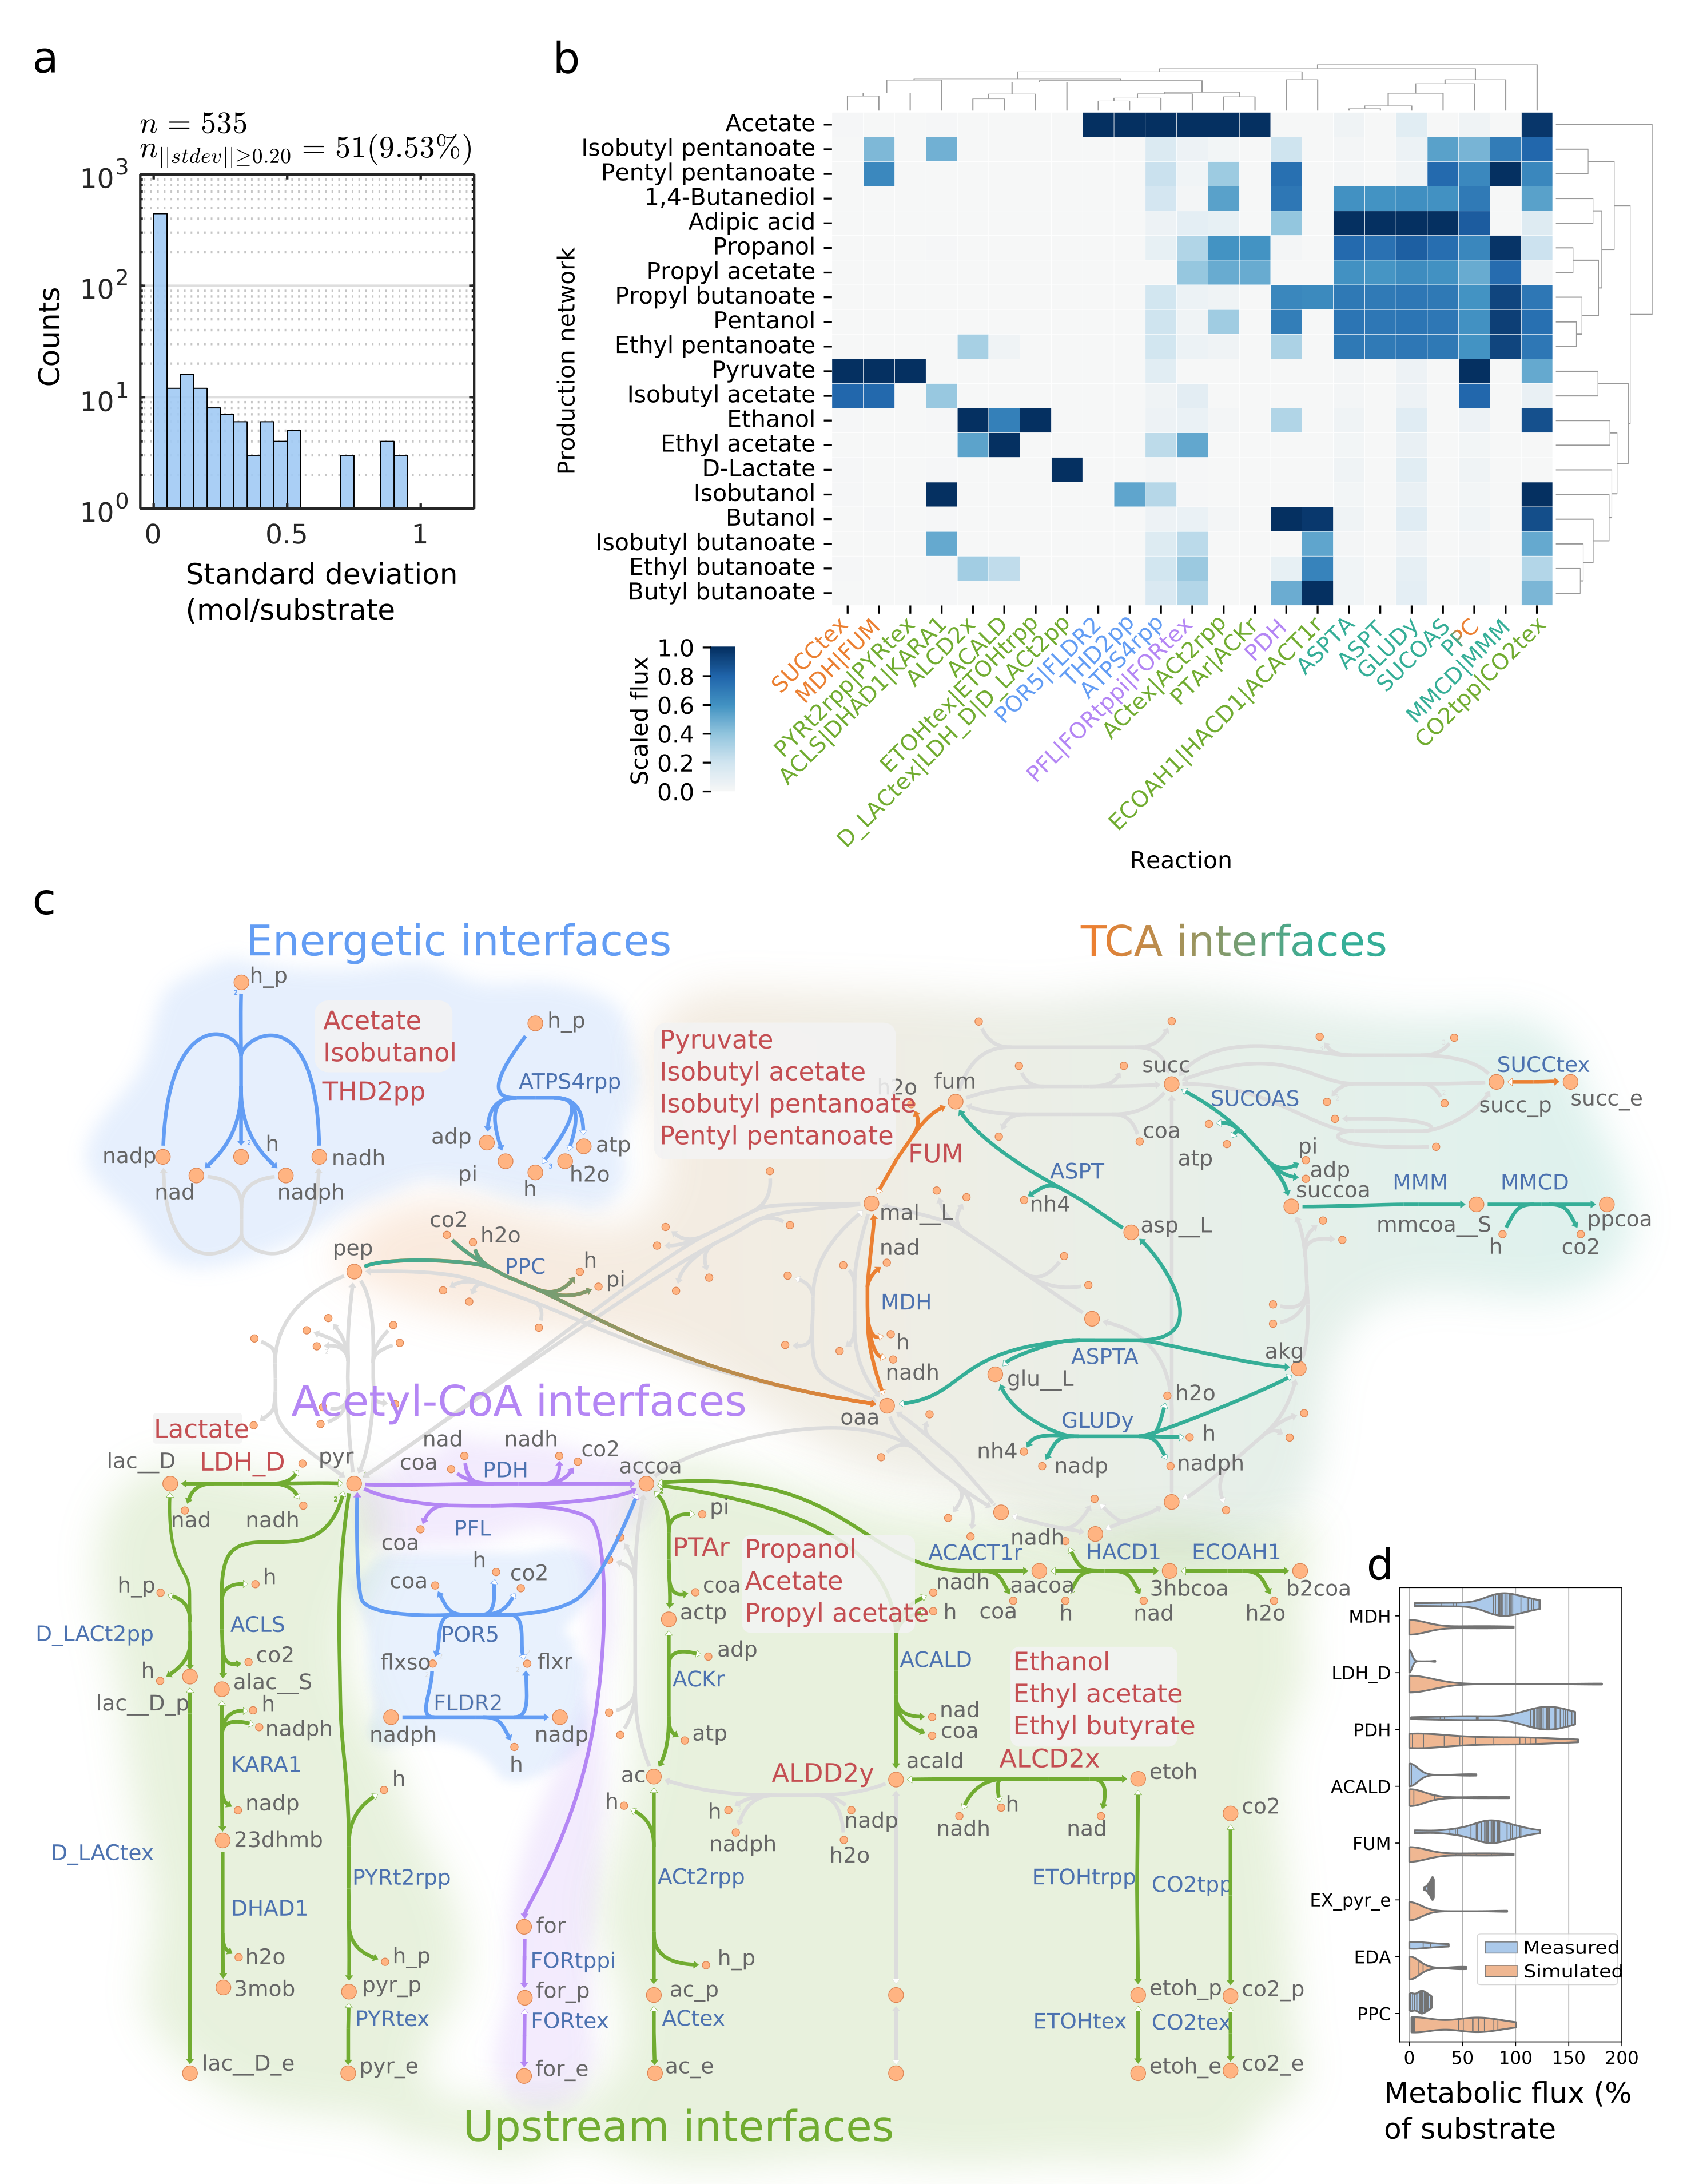
\includegraphics[height=\textheight,keepaspectratio]{core-modules.png}
%\end{figure}
%
%\addtocounter{figure}{-1}
\begin{figure}[!hp]
    \centering
    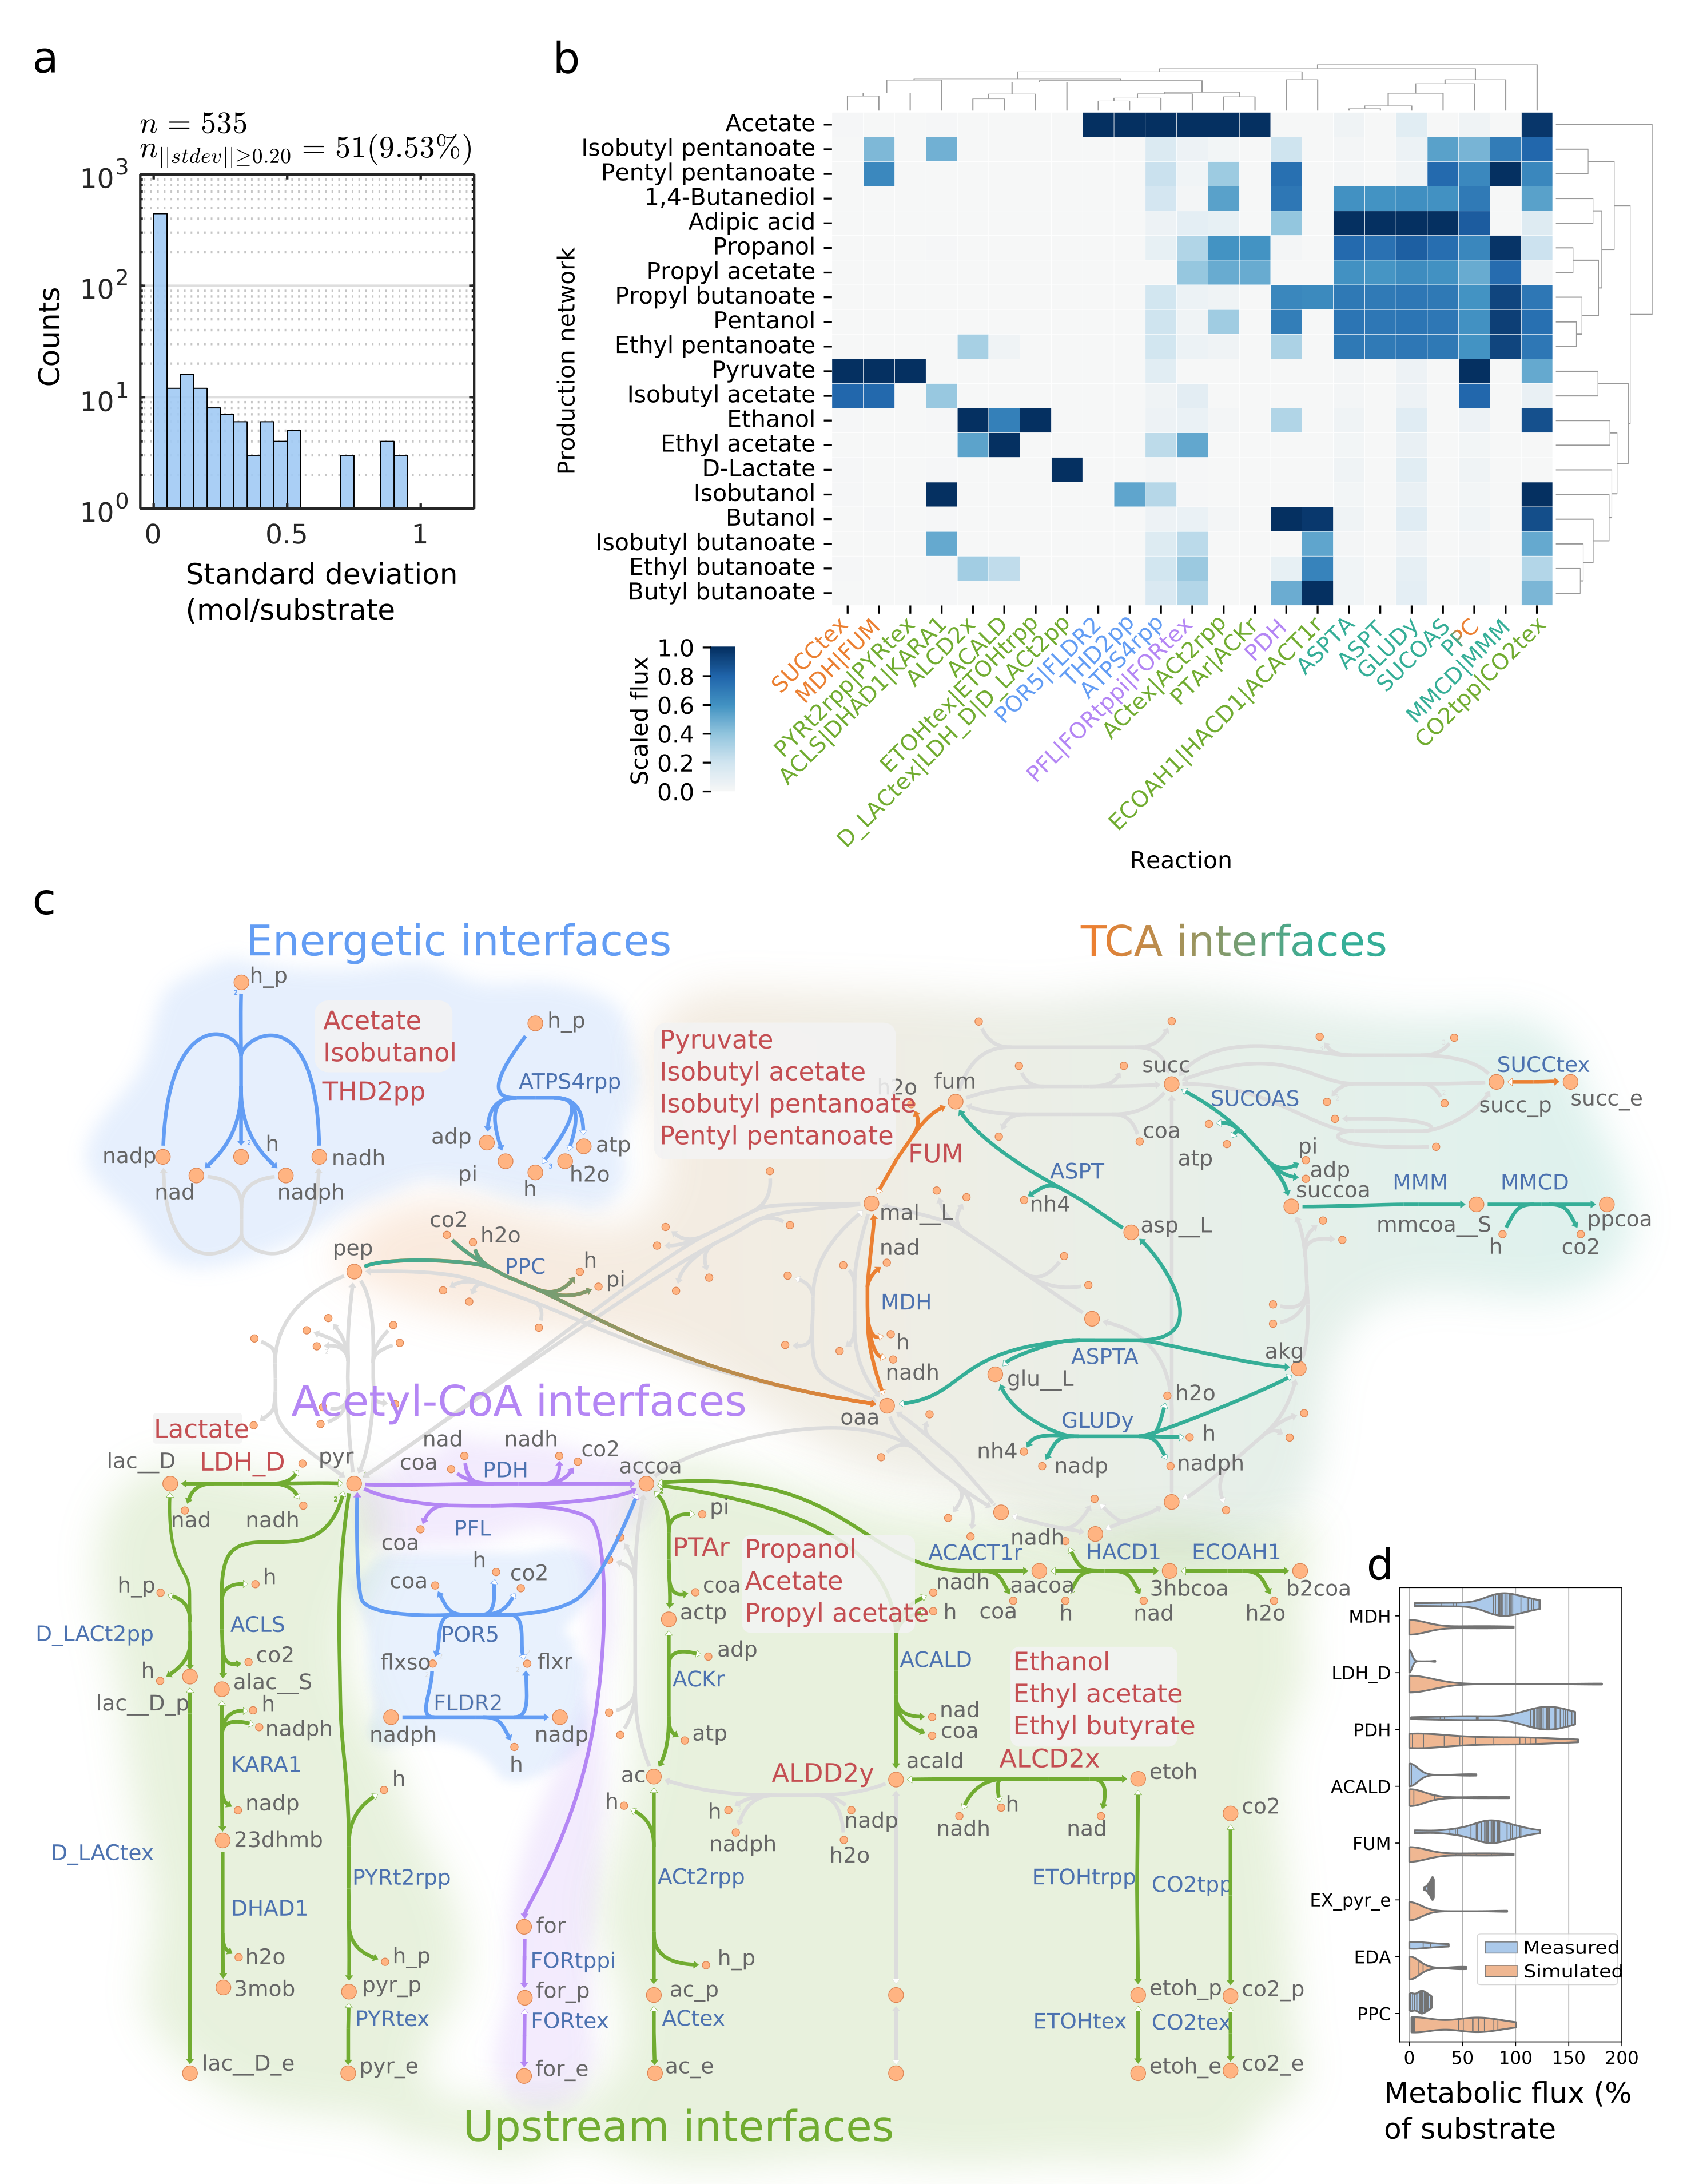
\includegraphics[height=.7\textheight,keepaspectratio]{core-modules.png}
    \caption[Flexible metabolic flux capacity of \textit{E. coli} metabolism enables the universal modular cell design]{Flexible metabolic flux capacity of \textit{E. coli} metabolism enables the universal modular cell design. (a) Standard deviation of each reaction flux  across production networks. (b) Scaled fluxes of the 51 reactions with standard deviation magnitude above 0.2,  excluding proton, water transport, and exchange reactions. A scaled flux for a reaction is determined by the reference flux distribution value divided by the maximum value of that reaction across all production networks. Hence, a scaled flux of 0 indicates a given reaction does not carry any flux, and a scaled flux of 1 indicates that this reaction carries the highest flux across production networks.  Several columns have multiple reactions, separated by $\vert$, since they carry exactly the same flux. (c) Endogenous modules of the universal modular cell.  The reactions colored in red are deleted in the chassis, but are used as module reactions in the production networks shown in the adjacent gray boxes. Metabolites in periplasmic and extracellular compartments have ``\_p" and ``\_e" suffixed to their abbreviations, respectively. Metabolite and reaction abbreviations follow BiGG\citep{king2015} notation.  (d) Comparison between simulated and measured fluxes. The solid lines within the ``violins" correspond to samples.
    %The simulated fluxes for the  reversible reactions, including FUM, LDH, MDH, and ACALD, were multiplied by -1 to reflect their most common direction.
    }%\textit{Figure on previous page.}}
    \label{fig5:core-modules}
\end{figure}
%}

\subsubsection{Comparison between simulated and measured intracellular fluxes reveals flexible metabolic flux capacity of \textit{E. coli} to accommodate the required wide flux ranges} \label{sec:flux_comparison}

Flux analysis of the production networks suggests that the core metabolic reactions (Figure~\ref{fig5:core-modules}b) require a wide range of fluxes when coupled with different production modules. To successfully implement this modular design in practice, we need to evaluate whether the metabolism of \textit{E. coli} has the inherent metabolic flux capacity to accommodate these required fluxes.
We compared the simulated reference flux distributions with a recent collection of 45 measured metabolic fluxes \citep{khodayari2016} that are collected from multiple studies across various conditions (e.g., growth under aerobic and anaerobic conditions, use of glucose or acetate or pyruvate as a carbon source) and genotypes (e.g., wild-type \textit{E. coli} and mutants with single gene deletions) \citep{ishii2007, kabir2005, zhao2004, zhao2003}.
Note that while the experimental data set provides a flux distribution baseline for wild-type and relatively small deviations for single gene deletion mutants, we anticipate that highly engineered strains with more gene deletions are likely to exhibit wider flux distributions.

Within the reactions present in the 23 groups that constitute endogenous modules (Figure~\ref{fig5:core-modules}b), 8 reactions also appeared in the experimental dataset (Figure~\ref{fig5:core-modules}d).
Remarkably, a highly consistent overlap of flux ranges was observed between the simulated and measured fluxes for malate dehydrogenase (MDH), pyruvate dehydrogenase (PDH), acetaldehyde dehydrogenase (ACALD), fumarase (FUM), and 2-dehydro-3-deoxy-phosphogluconate aldolase (EDA).
For the cases of  D-lactate dehydrogenase (LDH\_D), and pyruvate secretion (EX\_pyr\_e) that are directly coupled with the biosynthesis of lactate and pyruvate, respectively, we observed the maximum simulated fluxes surpass the measured values, suggesting that further engineering of wild-type and single-gene deletion \textit{E. coli} is needed to attain the requried fluxes.
Indeed, previous studies\citep{zhou2003, causey2004} have been able to redirect metabolic fluxes in \textit{E. coli} for yields of lactate and pyruvate above 75\% of the theoretical maximum values by simultaneous elimination of competing fermentative pathways for biosynthesis of acetate ($\Delta$\textit{ackA}), formate ($\Delta$\textit{pflB}), and ethanol ($\Delta$\textit{adhE}).
The only remaining discrepancy between the simulated and measured fluxes is PPC.
Studies, not included in the comparison data set, have reported up to 50\% more PPC flux observed under aerobic conditions \citep{peng2004, siddiquee2004}, which is still considerably below several of the simulated fluxes.
This result suggests that PPC can be a potential metabolic bottleneck in certain production modules. One possible solution is to include in the affected production modules the heterologous PPC from \textit{Actinobacillus succinogenes} which has been successfully over-expressed in \textit{E. coli} for increased succinate production \citep{kim2004}.
Additionally, bacterial PPC activity can be increased by elevating the acetyl-CoA pool \citep{lin2004}.


% Note: Most of the fluxes are aerobic, which may explain some of the bias in particular with LDH_D, however this can also be a source of challenge, since the design is anaerobic. Also the fluxes of engineered strains with most fermentative products remove can be very different, and such strains are not necessarily included here, but the type of strain we are analyzing has 6 knockouts. Also some fluxes in W.T. seem to be widely different among studies.

\subsubsection{Random sampling of metabolic fluxes confirms the narrow operation range of endogenous modules}
The reference flux distributions analyzed so far represent the ideal metabolic states for each production strain. However, other metabolic states might also exist.
To address this uncertainty, we performed randomized flux sampling \citep{kaufman1998, heirendt2017} for each production network under the constraint that product synthesis rate must be above 50\% of the maximum value.
The results show that the metabolic flux distributions (Figure~\ref{fig5:fig-s2}) for most reactions involved in the endogenous modules are very narrow, except for the two alternative pathways of ethanol biosynthesis, i.e., the endogenous PDH-ACALD-ALCD2x route comprising of pyruvate dehydrogenase, acetaldehyde dehydrogenase, and alcohol dehydrogenase (Figure~\ref{fig5:sampling}a) and the heterologous PYRDC-ALCD2x route comprising of pyruvate decarboxylase and alcohol dehydrogenase. These two pathways can be used interchangeably in the ethanol production network, where there is a linear correlation between PYRDC and PDH fluxes (Figure~\ref{fig5:sampling}b). Notably, the sampled fluxes cannot indicate preferential use of either the ethanol synthesis route because the model does not take into account of kinetic ($k_{\textrm{cat}}$, $k_\textrm{M}$) and regulatory constraints.
%Furthermore, the sampled fluxes do not capture the extremes where only of the two alternative pathways is used, this could be indicative of a possible biological phenomenon or introduced by a bias in flux sampling towards high volume regions of the solution space.
In summary, even though reactions in the endogenous modules must have flexible metabolic flux capacities to enable a universal modular cell to be compatible with various exchangeable production modules, they must also operate within in a narrow flux range when interfacing with a specific production module.

%\afterpage{%
%\paragraph{Figure S2}
\begin{figure}[!hp]
    \centering
    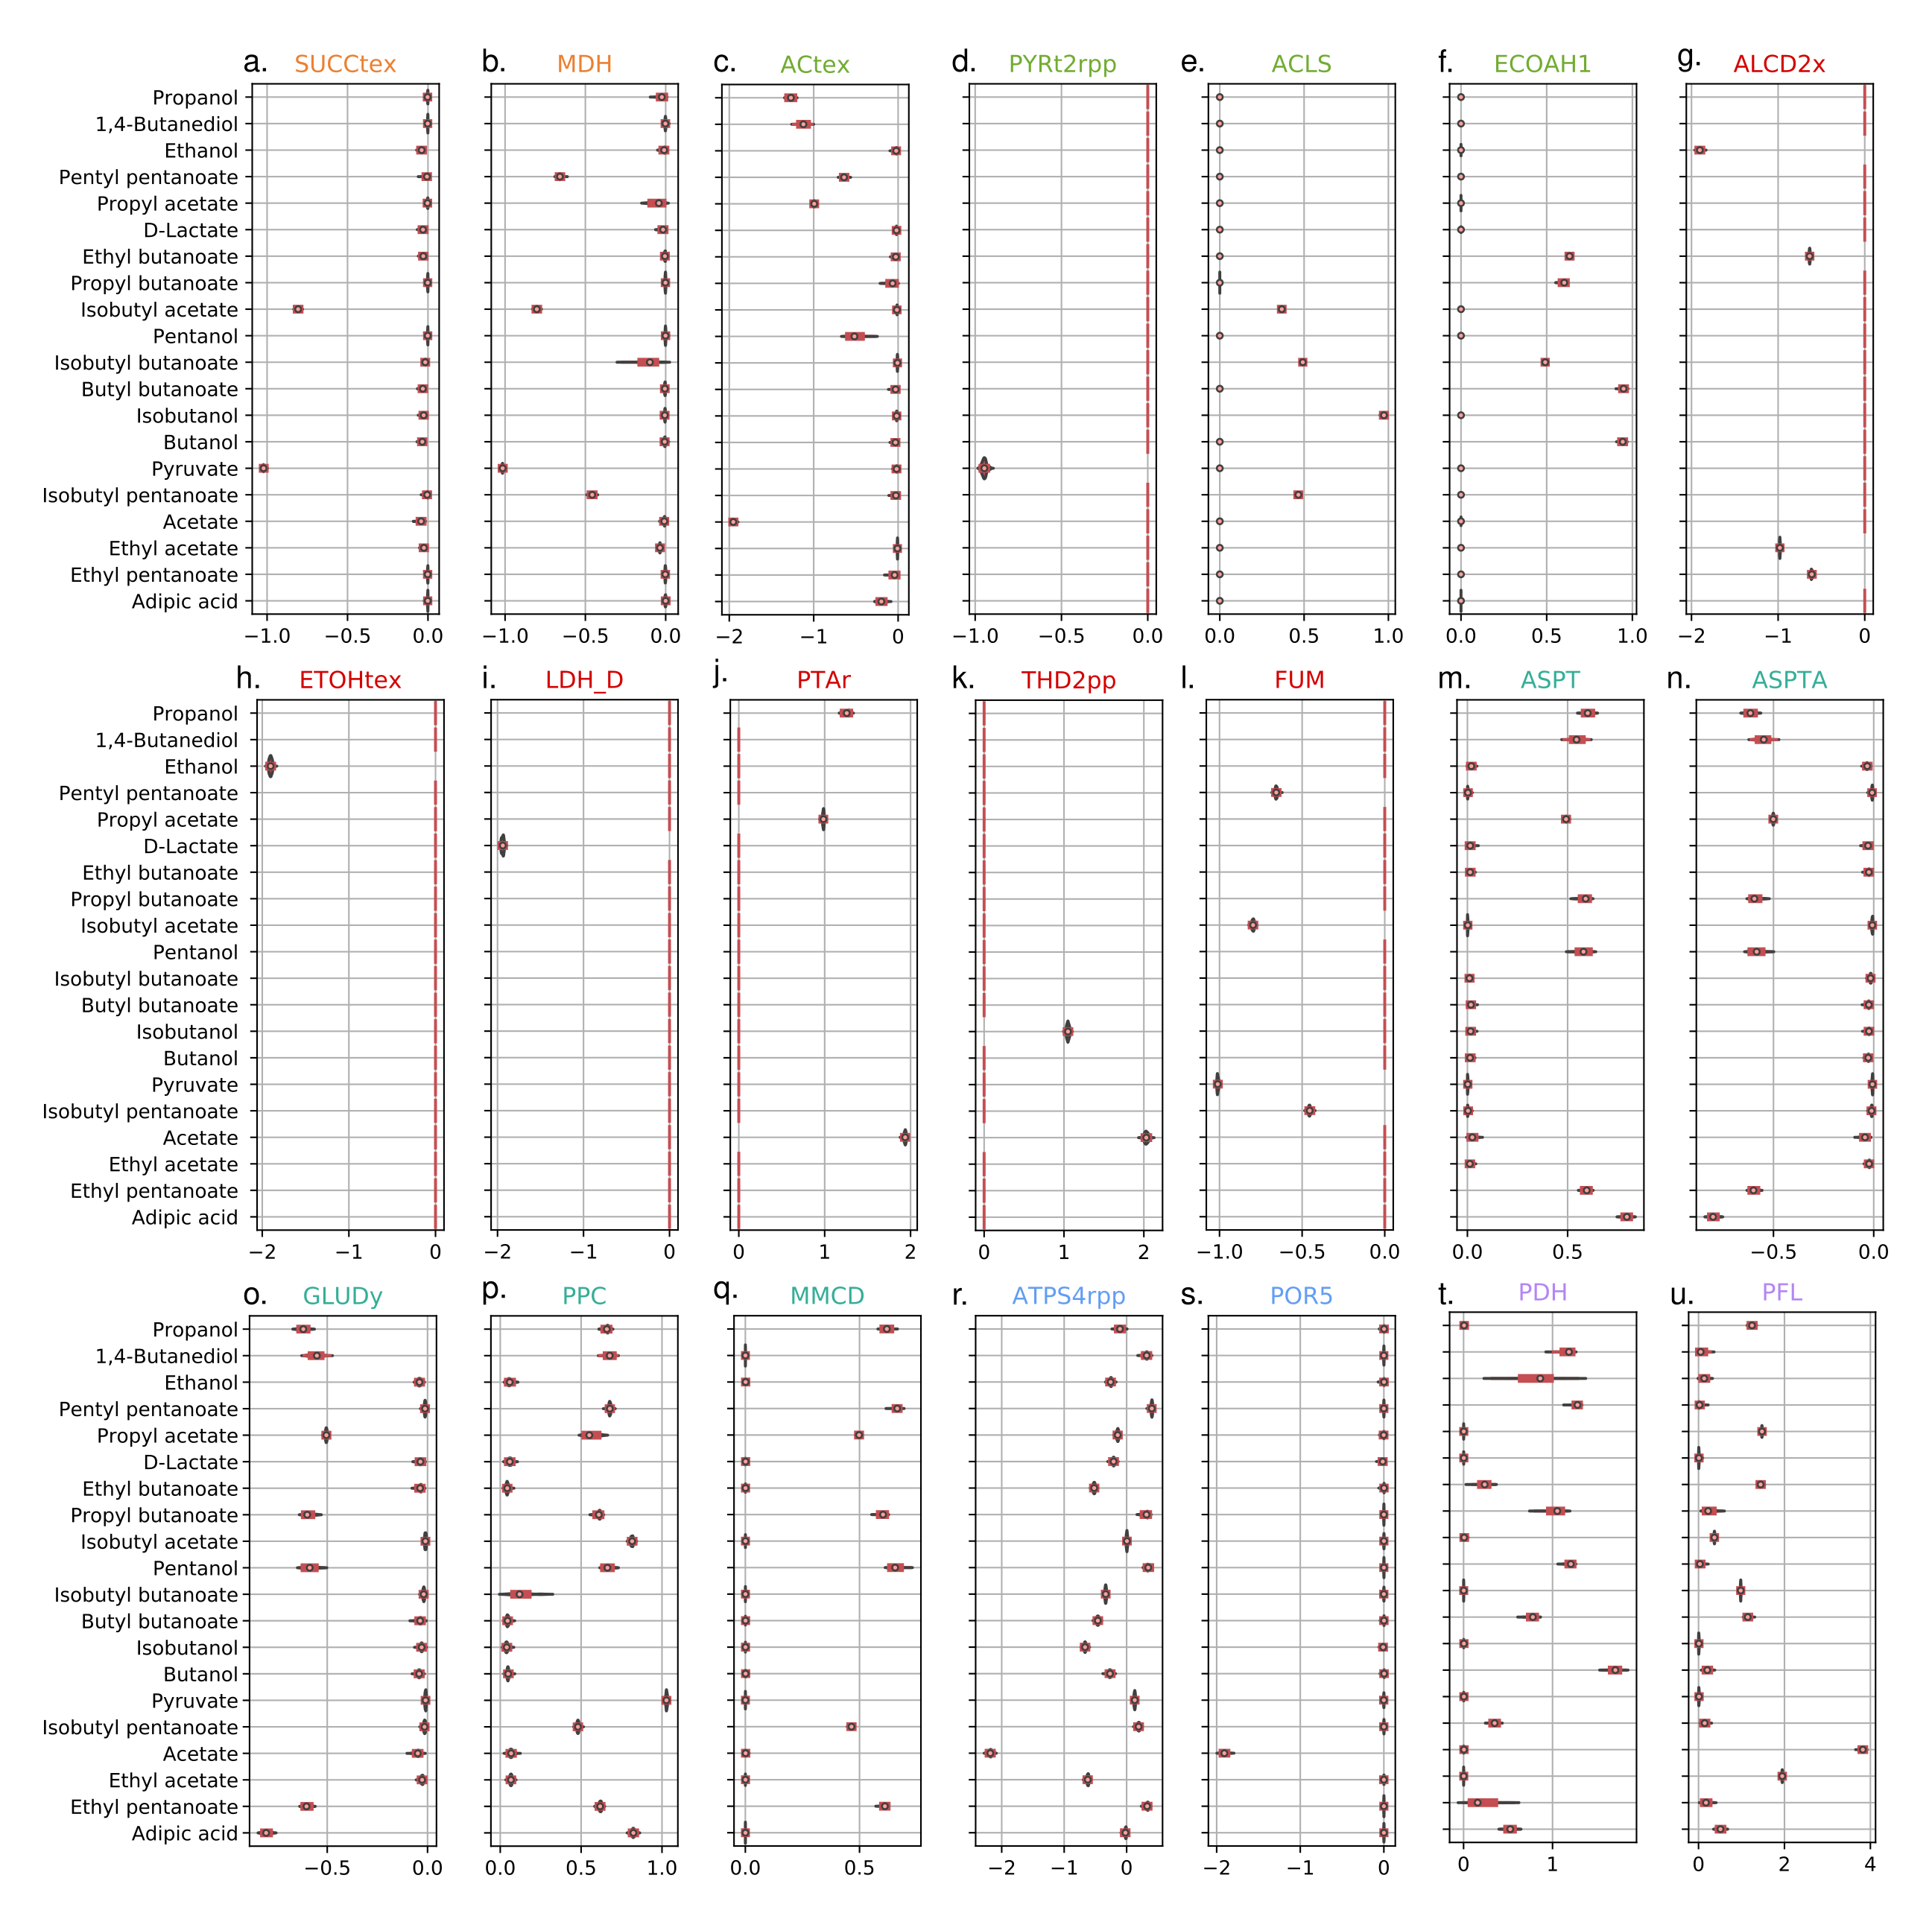
\includegraphics[width=\textwidth,height=\textheight,keepaspectratio]{Figure-S2}
    \caption[Violin plot of sampled reaction flux distributions]{
Violin plot of sampled reaction flux distributions. Reaction colors are consistent with Figure~\ref{fig5:core-modules}. The flux of SUCOAS could not be sampled since this reaction is involved in a thermodynamically infeasible cycle.
    }
    \label{fig5:fig-s2}
\end{figure}
%}

%\afterpage{%
\begin{figure}[!ht]
    \centering
    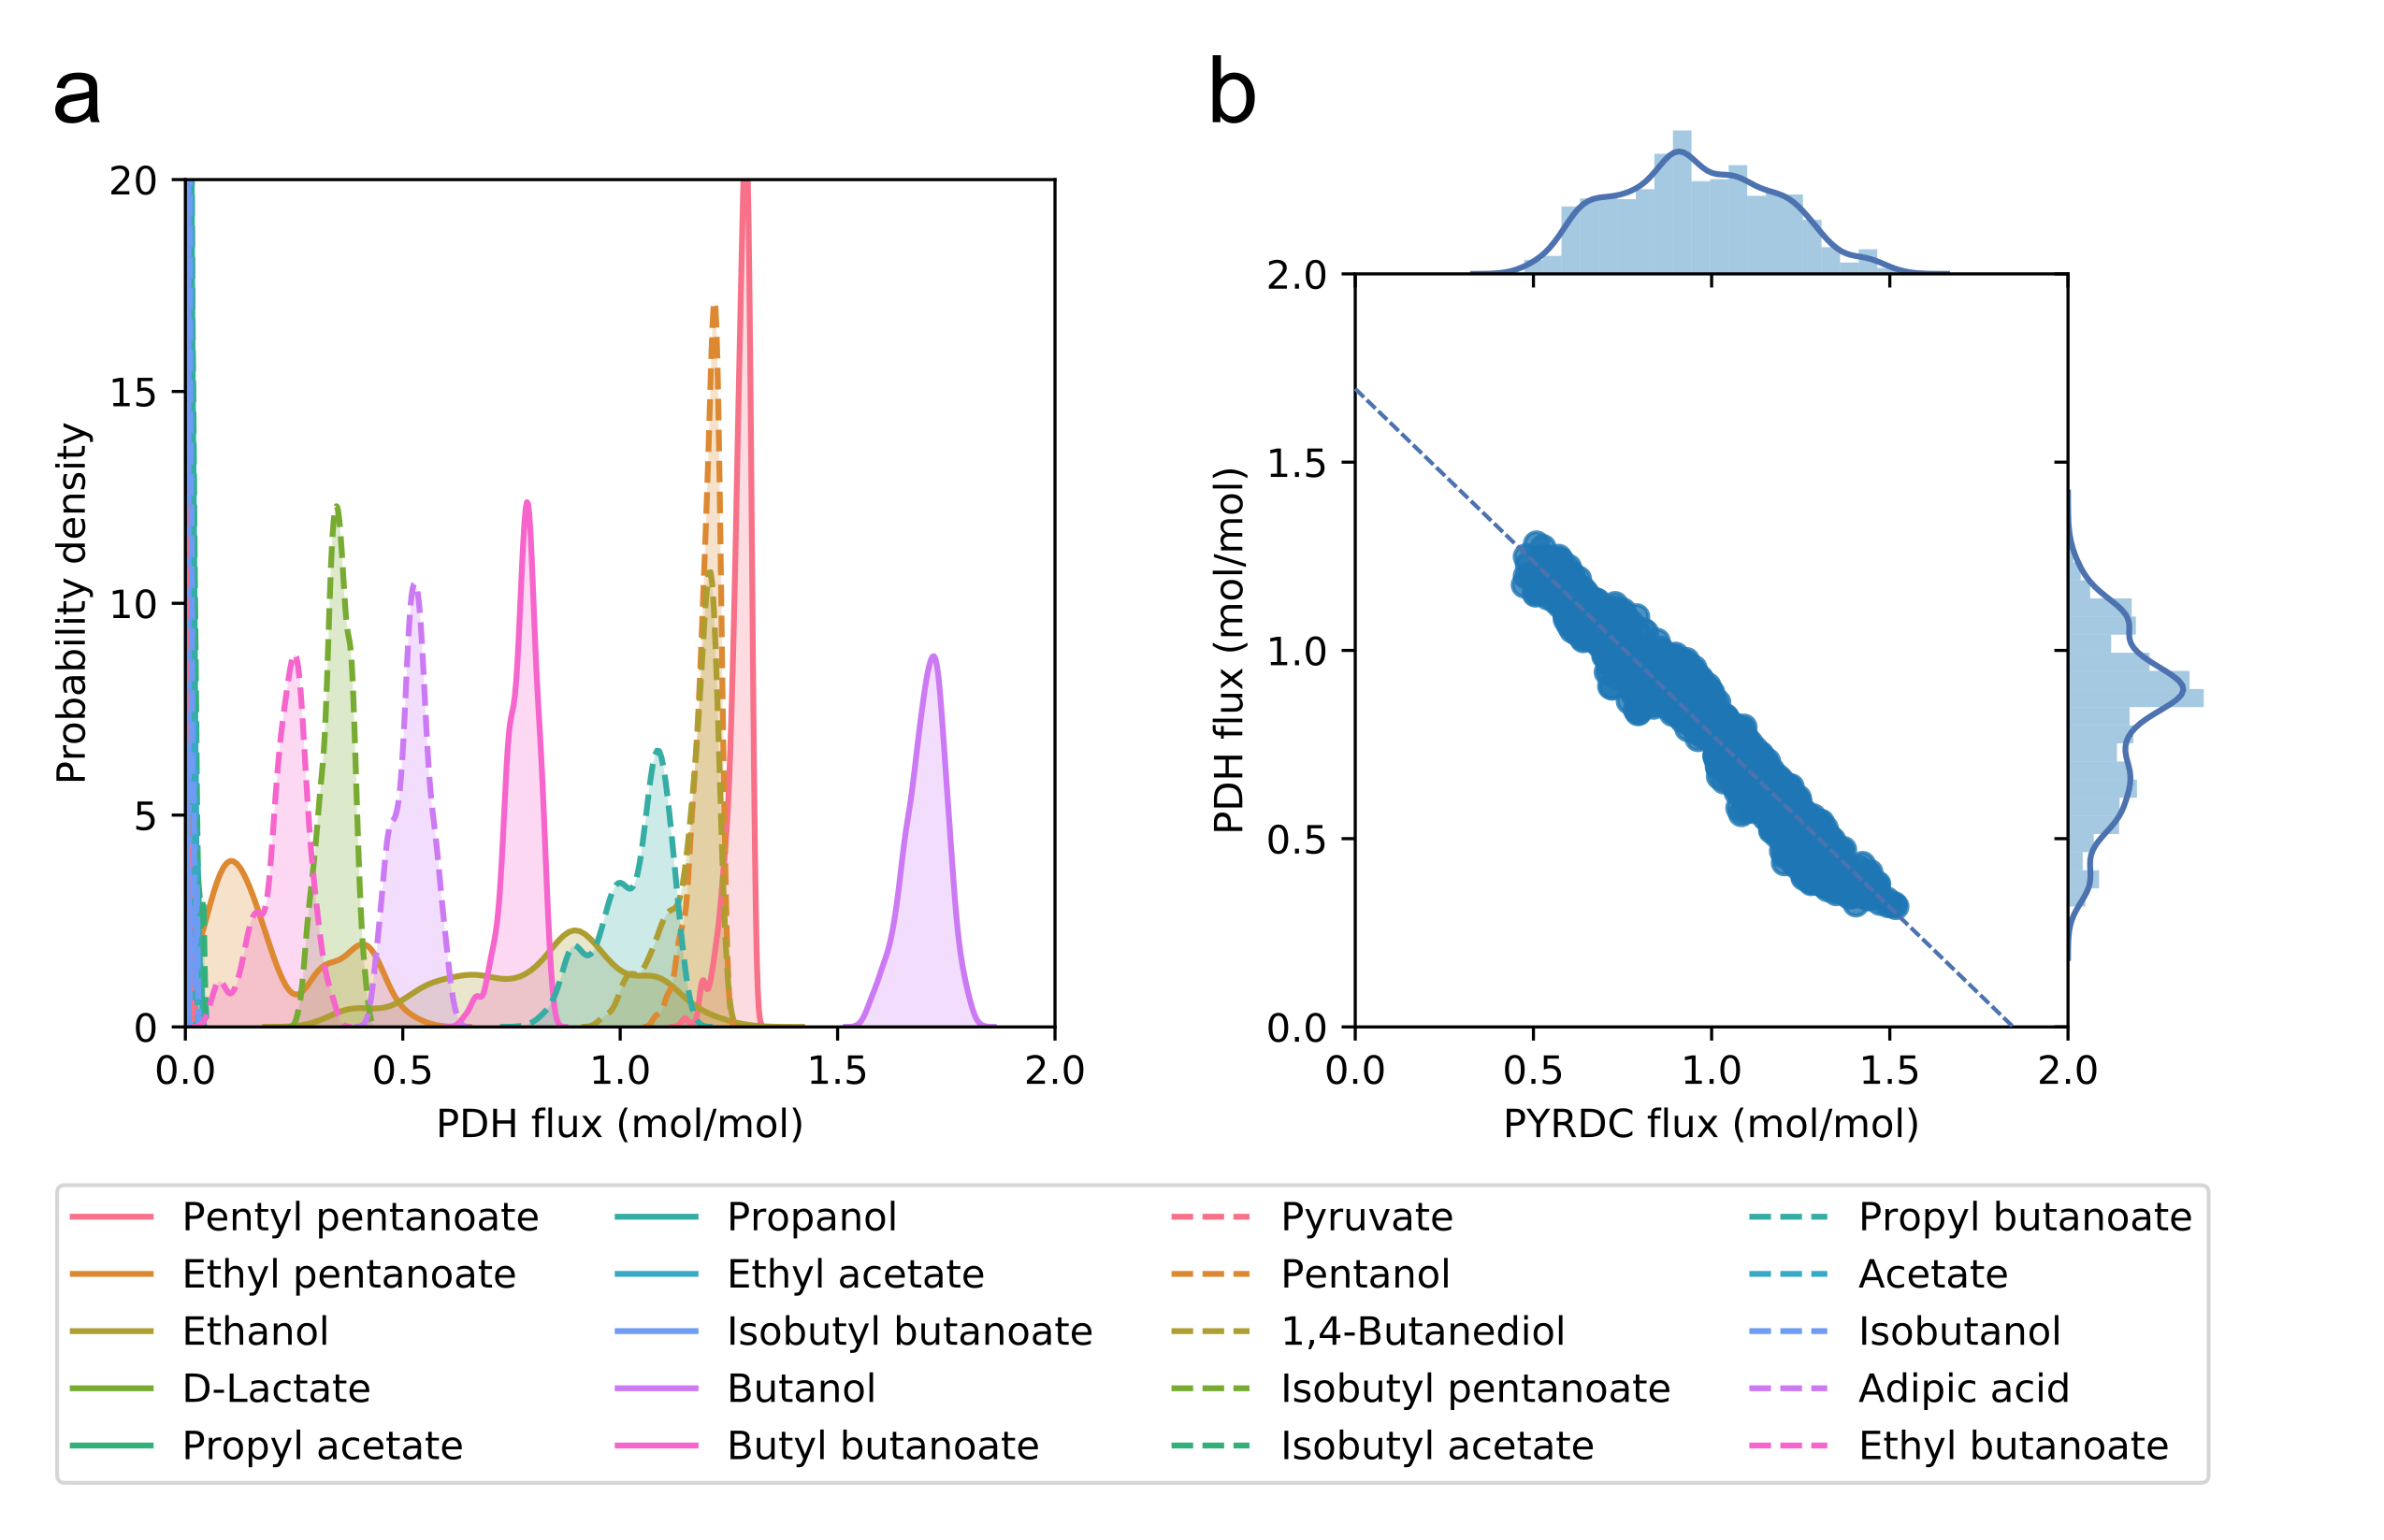
\includegraphics[width=.9\textwidth,keepaspectratio]{ethanol_sampling.png}
    \caption[Sampled flux distributions of the ethanol biosynthesis pathways]{Sampled flux distributions of the ethanol biosynthesis pathways. (a)~Probability density function of sampled fluxes for pyruvate dehydrogenase (PDH) across all production networks. Note that ethanol and ethyl pentanoate have the widest operation range. (b)~Sampled metabolic fluxes of pyruvate decarboxylase (PYRDC) and PDH in the ethanol production network.}
    \label{fig5:sampling}
\end{figure}%}


\section{Conclusions}
In this study, we formulated multi-objective modular strain design as blended and goal attainment optimization problems. These problems can be solved by MILP algorithms that guarantee Pareto optimal solutions, exhaustively search the space of alternative solutions, and specify design requirements such as module prioritization or universal compatibility.
This multi-objective strain design approach can be extended with additional design variables (e.g., up- and down-regulation\citep{pharkya2004} or reaction insertion from database\citep{pharkya2006}) or alternative flux prediction models\citep{chowdhury2014,dinh2018} to expand its applications, including use of exchangeable metabolic modules for bioremediation  and biosensing.
In terms of biological significance, the ModCell2-MILP and FVC methods developed could identify a universal modular cell that harnesses the inherent modularity and flexibility of native \textit{E. coli} metabolism to properly interface with a variety of biochemically diverse pathways. This universal design was predicted to display a growth-coupled-to- product-formation phenotype for all pathways, enabling its use as a platform for pathway optimization through high-throughput library selection and/or adaptation. The feasibility of this universal design strategy is found to be consistent with experimental evidence of isolated metabolic engineering strategies towards target products and measured intracellular flux ranges. Furthermore, analysis of the metabolic fluxes in this universal design revealed clusters of reactions in central metabolism, named endogenous modules, that become activated to interface with specific pathways, providing a mechanistic view into the modularity of metabolic pathways.
In this study, the universal design developed was limited to a library of 20 molecules in \textit{E. coli} because one primary aim was to compare the MILP solution with the MOEA solution previously presented. Future studies will use the developed methods to design and understand modularity for different organisms and a larger library of product synthesis modules.


% Include only the SI item label in the paragraph heading. Use the \nameref{label} command to cite SI items in the text.
\section*{Supporting information}

\paragraph{File S1}
\textbf{Spreadsheet with modular cell designs for \textit{E. coli} core model.}

\paragraph{File S2}
\textbf{Computer programs used to generate the results of this study.}






%\section{Acknowledgments}
%This research was funded by the NSF CAREER Award (NSF\#1553250) and the Center of Bioenergy Innovation (CBI), U.S. Department of Energy Bioenergy Research Center supported by the Office of Biological and Environmental Research in the DOE Office of Science. The funders had no role in the study design, data collection and analysis, decision to publish, or preparation of the manuscript.
%

%\section*{Author contributions}
%Conceptualization: SG, CT; Data Curation: SG; Formal Analysis: SG; Funding Acquisition: CT; Investigation: SG; Methodology: SG; Project Administration: CT;  Resources: CT; Software: SG; Supervision: CT; Validation: SG, CT; Visualization: SG, CT; Writing: SG; Writing – Review \& Editing: SG, CT.

\section{Definitions} \label{sec:definitions}
\paragraph{Sets}
\begin{description}[leftmargin=1.5cm, style=nextline, itemindent=-10pt]
\item[$\mathcal{I}_k$] Metabolites in production network $k$.
\item[$\mathcal{J}_k$] Reactions in production network $k$.
\item[$\mathcal{K}$]  Production networks that are derived from a combination of the parent metabolic network with the metabolic pathways associated with production modules. The parent metabolic network is the network of the host strain that is genetically manipulated to build a modular cell chassis.
\item[$\mathcal{M}$] Metabolic states that correspond to the growth phase, denoted $\mu$, and the non-growth or stationary phase, denoted $\bar{\mu}$.
\item[$\mathcal{C}$] Candidate deletion reaction set. The removal of these reactions are applied to all production networks, $\mathcal{C} \subseteq \mathcal{J}^{\textrm{parent}} \subseteq \mathcal{J}_k, \; \forall k \in \mathcal{K}$.
\item[$\mathcal{N}_k$] Non-targeted deletion reaction set in production network $k$. This set arises from the use of fixed endogenous module reactions $z_{jk}$ in certain production networks.
\end{description}

\paragraph{Binary variables}
\begin{description}[leftmargin=1.5cm, style=nextline, itemindent=-10pt]
\item[$y_j$] Reaction deletion indicator that takes a value of 0 if reaction $j$ is deleted in the chassis and 1 otherwise.
\item[$z_{jk}$] Endogenous module reaction indicator that takes a value of 1 if reaction $j$ is added back as module reaction in production network $k$ and 0 otherwise.
\item[$d_{jk}$] Reaction activity indicator that takes a value of 0 if reaction $j$ in production network $k$ might not carry a flux and 0 otherwise, thus $d_{jk} = y_j \lor z_{jk}$. This variable is declared as a continuous and linear constraints enforce the OR relation and thus makes the variable binary.
\item[$w_k$] Production network feasibility indicator that takes a value of 0 if reaction deletions are ignored and the objective value is set to 0 for production network $k$, and a value of  1 otherwise.
\item[$e_{jk}$]  Reaction activity indicator adjusted to $w_k$ that takes the value of $d_{jk}$ if $w_k=1$ and a value of 1 if $w_k=0$, thus $e_{jk}=(d_{jk}\land w_k) \lor \lnot w_k$.
\item[$r_{jk}$] Linearization variable, $r_{jk} = d_{jk} \lor w_k.$
\end{description}

\paragraph{Continuous variables}
\begin{description}[leftmargin=1.5cm, style=nextline, itemindent=-10pt]
\item[$v_{jkm}$] Flux (mmol/gCDW/hr) of reaction $j$ from network $k$ at metabolic state $m$.
\item[$v_{Pkm}$] Flux (mmol/gCDW/hr) of product synthesis reaction from network $k$ at metabolic state $m$.
\item[$v_{Xkm}$] Flux (mmol/gCDW/hr) of biomass synthesis reaction from network $k$ at metabolic state $m$.
\item[$f_k$] General objective function for production network $k$ that can be represented by $f_k^{wGCP}$, $f_k^{lsGCP}$, or $f_k^{NGP}$.
\item[$f_k'$] Objective function adjusted by $w_k$ such that $f_k'$ = $f_k$ if $w_k=1$ and $f_k'=0$ otherwise.
\item[$\delta_k^+$] Amount required by the objective value $f_k'$ to attain the target goal $g_k$,  i.e.. $\delta_k^+ = g_k - f_k$ if $f_k' < g_k$.
\item[$\delta_k^-$] Amount that the objective value $f_k'$ surpasses the target goal $g_k$, i.e., $\delta_k^- = f_k' - g_k$ if $f_k' > g_k$.
\item[$\lambda_{ikm}$] Dual variable associated with mass balance constraint of metabolite $i$ from production network $k$ at growth state $m$.
\item[$\mu_{jkm}^{l}$] Dual variable  associated with the lower bound of reaction $j$ from production network $k$ at growth state $m$.
\item[$\mu_{jkm}^{u}$] Dual variable  associated with the upper bound of reaction $j$ from production network  $k$ at growth state $m$.
\item[$p_{jkm}^{l}$] Linearization variable, $p_{jkm}^{l}=e_{jk} \mu^{l}_{jkm}$.
\item[$p_{jkm}^{u}$] Linearization variable, $p_{jkm}^{u}=e_{jk} \mu^{u}_{jkm}$.
\end{description}

\paragraph{Parameters}
\begin{description}[leftmargin=1.6cm, style=nextline, itemindent=-10pt]
\item[$S_{ijk}$] Stoichiometric coefficient of metabolite $i$ in reaction $j$ of production network $k$.
\item[$l_{jkm}$] Lower bound for reaction $j$ of production network $k$ at metabolic state $m$.
\item[$u_{jkm}$] Upper bound for reaction $j$ of production network $k$ at metabolic state $m$.
\item[$\gamma$] Minimum biomass synthesis rate required for growth states. Note that in this study a conservative value of 20\% of the maximum predicted growth rate of the wild-type strain was used to generate all results.
\item[$\alpha$] Maximum number of deleted reactions in the modular cell chassis.
\item[$\beta_k$] Maximum number of endogenous module reactions in production network $k$.
\item[$\epsilon$] Small scalar used for tilting the biomass objective function, leading to the minimum product rate available at the maximum growth rate. Note that in our study $\epsilon=0.0001$ was used to generate all results.
\item[$b_{\mu}$, $b_{\bar{\mu}}$] Weights on the growth  and non-growth objectives of $f_k^{lsGCP}$, respectively. Note that in our study  $b_{\mu}=1$ and $b_{\bar{\mu}}=10$ were used to generate all results.
\item[$a_k$] Weighting factor applied to the objective function for production network $k$ in the  blended formulation. Note that in our study $a_k =1, \; \forall k \in \mathcal{K}$ was used unless otherwise noted.
\item[$g_k$] Target value for objective $f_k'$ in the goal programming formulation.
\item[$a_k^+$] Weighting factor applied to $\delta_k^+$ which emphasizes the importance of objective value $f_k'$ to avoid falling below the target value $g_k$. Note that in our study $a_k^+ = 1, \; \forall k \in \mathcal{K}$ was used in all cases.
\item[$a_k^-$] Weighting factor applied to $\delta_k^-$ which emphasizes the importance of the objective $f_k'$ to avoid surpassing the target value $g_k$. Note that in our study $a_k^- = 1, \; \forall k \in \mathcal{K}$ was chosen everywhere except to determine the universal modular cell design, where $a_k^- = 0, \; \forall k \in \mathcal{K}$ was used.
\item[$M^w$] Determines the minimum value of $f_k$ that allows $w_k$ to not be 0. A value of 10, corresponding to $f_k \ge 0.01$ for $w_k \ne 0$, was used in all cases.
\item[$M^{obj}$] Upper bound for each objective value. Note that in our study a value of 20 was set for all cases.
\item[$M$] Upper bound for dual variables. Note that in our study a value of 100 was set for all cases.
\end{description}

%\bibliography{bibliography}
%\end{document}




    \chapter{Genome-scale metabolic network reconstruction of \textit{C. thermocellum} to design modular cells for consolidated bioprocessing} \label{ch:ctherm}

\disclose{Development of an updated genome-scale metabolic model of Clostridium thermocellum and its application for integration of multi-omics datasets. Garcia, S., Thompson, R.A., Giannone, R. J., Dash, S., Maranas , C. D., and Trinh, C. T. In preparation, 2019}

    \chapter{Design of modular cells for large product libraries}
%\chapter{Development of method to design modular cells with many objectives and its application to identify generalized modular cell design principles}
\label{ch:hpc}

\disclose{Top-down design of microbial catalysis platforms for large libraries of product synthesis modules. Garcia, S. and Trinh, C. T. In preparation, 2020}

\section*{Abstract}
    % 1. Intro
    Microbial metabolism can be engineered to produce many useful chemicals from renewable resources such as plant biomass.
    % 2. Problem/research question
    However, this technology remains economically unfeasible for most target chemicals due to the large amount of time and resources required to develop microbial catalysts for each new product.
    % 3 What is lacking
    To tackle this challenge, metabolic engineers have gained recent interest in the construction of platform strains that can avoid redundant efforts and increase system robustness, transferring the proven advantages of modular design to cellular biocatalysis.
    % 3
    In particular, we have recently proposed modular cell (ModCell) design, a method to systematically build a chassis that can readily couple with modules that enable phenotypes like target molecule overproduction.
    % 3 / 4 (why care about looking at more products to address the original challenge
    However, previous ModCell design methods were limited to libraries of up to 20 products, but the potential number of products for modular biocatalysts is much larger due to the biochemical diversity of nature.
    % 5 approach
    In this study, we develop ModCell-HPC, a method to design modular platform strains compatible with libraries of hundredths of product synthesis modules, and apply it to design \textit{E. coli} modular cells compatible with a library of 161 production modules under various carbons sources.
    We identify three \textit{E. coli} platform strains with few genetic manipulations that can cover total of 85 products for growth-coupled production.
    These designs not only include removal of major byproducts, but also alter key metabolic branch-points in central metabolism.
    We also use ModCell-HPC to identify the design features that allow an existing strain to be repurposed towards production of new molecules.
   % production of new to be re design modular cells under different carbon sources and to identify the features that make a strain compatible towards products unknown at the time of design.
    %We also use ModCell-HPC to design modular cells under different carbon sources and to identify the features that make a strain compatible towards products unknown at the time of design.
    %The designs, consistent with isolated cases from the literature, not only relay Identify branch points in central metabolism as key targets for the design of platforms strains
    % Should separate aerobic from anaerobic conditions?
    Overall, ModCell-HPC is an effective tool towards more efficient and generalizable design of modular platform strains to reduce the R\&D cost of  biocatalysis.


\section{Introduction}
% Structure:
% - Motivation: Strain design challenges
% - Gap and proposed approach
% - Accomplishments(/goals) of the study
% - Need to justify the use of growth coupling (take from a previous paper) primarly as a pathway selection tool

% 1.Motivation
%   - State of modular design
%   - Metabolic engineering/modcell/biocatalysis
%   - Shortcomings?
Modular design has gained recent interest as an effective tool to understand and efficiently redesign cellular systems. \citep{garcia2019b}
In the field of metabolic engineering, that aims to manipulate cellular metabolism for novel application including renewable chemical synthesis, pathway-\citep{biggs2014} and system-level\citep{trinh2015,garcia2019,garcia2019c,garcia2019d} modularization strategies have been proposed to address the noncompetitive slow and expensive design-build-test cycles of microbial catalysts.\citep{nielsen2016}
Among system-level modularization strategies, the ModCell approach formulated modular strain design as a multi-objective optimization problem that uses stoichiometric models to simultaneously design the chassis and modules towards desirable phenotypes such as growth coupled to product synthesis or two-phase fermentation.\citep{garcia2019}
There is a vast number of potential molecules that could be manufactured using metabolically engineered microbes,\citep{trinh2016} and modular design principles and methods such as ModCell could be effective to harness this potential, but remain unexplored at such larger scales. %TODO: Maybe a bit unclear?

Previous efforts in computational modular strain design investigated libraries of up to 20 products primary derived from central metabolism.\citep{garcia2019,garcia2019d}
This small number of products is useful for an implementation point of view,  since each product synthesis pathway module remains time consuming to build. However, to generalize design rules for modular platform strains is necessary to increase the product library size.
This leads to many-objective multi-objective optimization problems, which are notoriously difficult to solve.\citep{ishibuchi2008, li2018}  %(mention GA/MOEA parallelization, but how this is not well established
%by increasing the library size%, %an order of magnitude,
%we can generalize design rules for modular platform strains.
Such problems are often solved with multi-objective evolutionary algorithms (MOEA), however parallelization schemes that harness the power of high-performance computing (HPC) remain largely unexplored in this field.
Fortunately, conventional genetic algorithms for single-objective problems have developed multiple approaches to harness HPC \citep{alba2013} that seem applicable to MOEA.\citep{martens2013, jozefowiez2005, garcia2016}


% 3. Accomplishments and impact (highlights, but not as specific)
In this study we developed ModCell-HPC, a parallel MOEA that uses HPC to solve problems with hundredths of objectives for modular platform strain design.
We use ModCell-HPC to design \textit{Escherichia coli} modular cell with endogenous metabolites as production modules that constitute
a highly diverse library of molecules derived from all regions of metabolism.
%Using endogenous metabolites as target products, not only provides a highly diverse library of molecules derived from all areas of metabolism, but can also reveal aspects of the theorized naturally existing modularity of metabolism.\citep{kitano2004,ma2003,csete2004,ravasz2002} %NOTE: Don't bring it up unless relvant
The resulting designs reveal the importance of manipulating branch points in central metabolism, and the need for different specialized chassis to ensure maximum coverage of products in the library. %NOTE: There is also module usage analysis
%type of manipulations required by certain product types like fatty acids.
Furthermore, we also identify the effect of different carbon sources in the design modular cells and the features that increase the potential of an existing strain to be repurposed towards new products.
%Among the identified designs, we observe emerging product families that require different chassis as a consequence of their diverging biochemical needs. We also identify branching points in central metabolism that are important to manipulate to build modular platform strains.
%Furthermore, we identify the differences between various carbon sources for platform strain design and the features that increase the potential of an existing platform strain to be repurposed towards new products.

% In this study: 1) Develop and implement a multi-objective optimization algorithm for many-objectives for high scalability in HPC; 2) Apply the algorithm to design modular cells for 100s of molecules in core metabolism; 3) Study the metabolic features of the designs to identify general design principles for platform strains; 4) Identify the universality of the proposed designs by evaluating their compatibility towards modules not present in the input 4)


\section{Methods}
\subsection{Modular cell design multi-objective optimization formulation}

\begin{figure}[hp]
    % TODO: Avoid too much narration and just explain what the pictures mean
    % TODO(figure):  lighten chassis color and darken Product 1 module color.
    \centering
    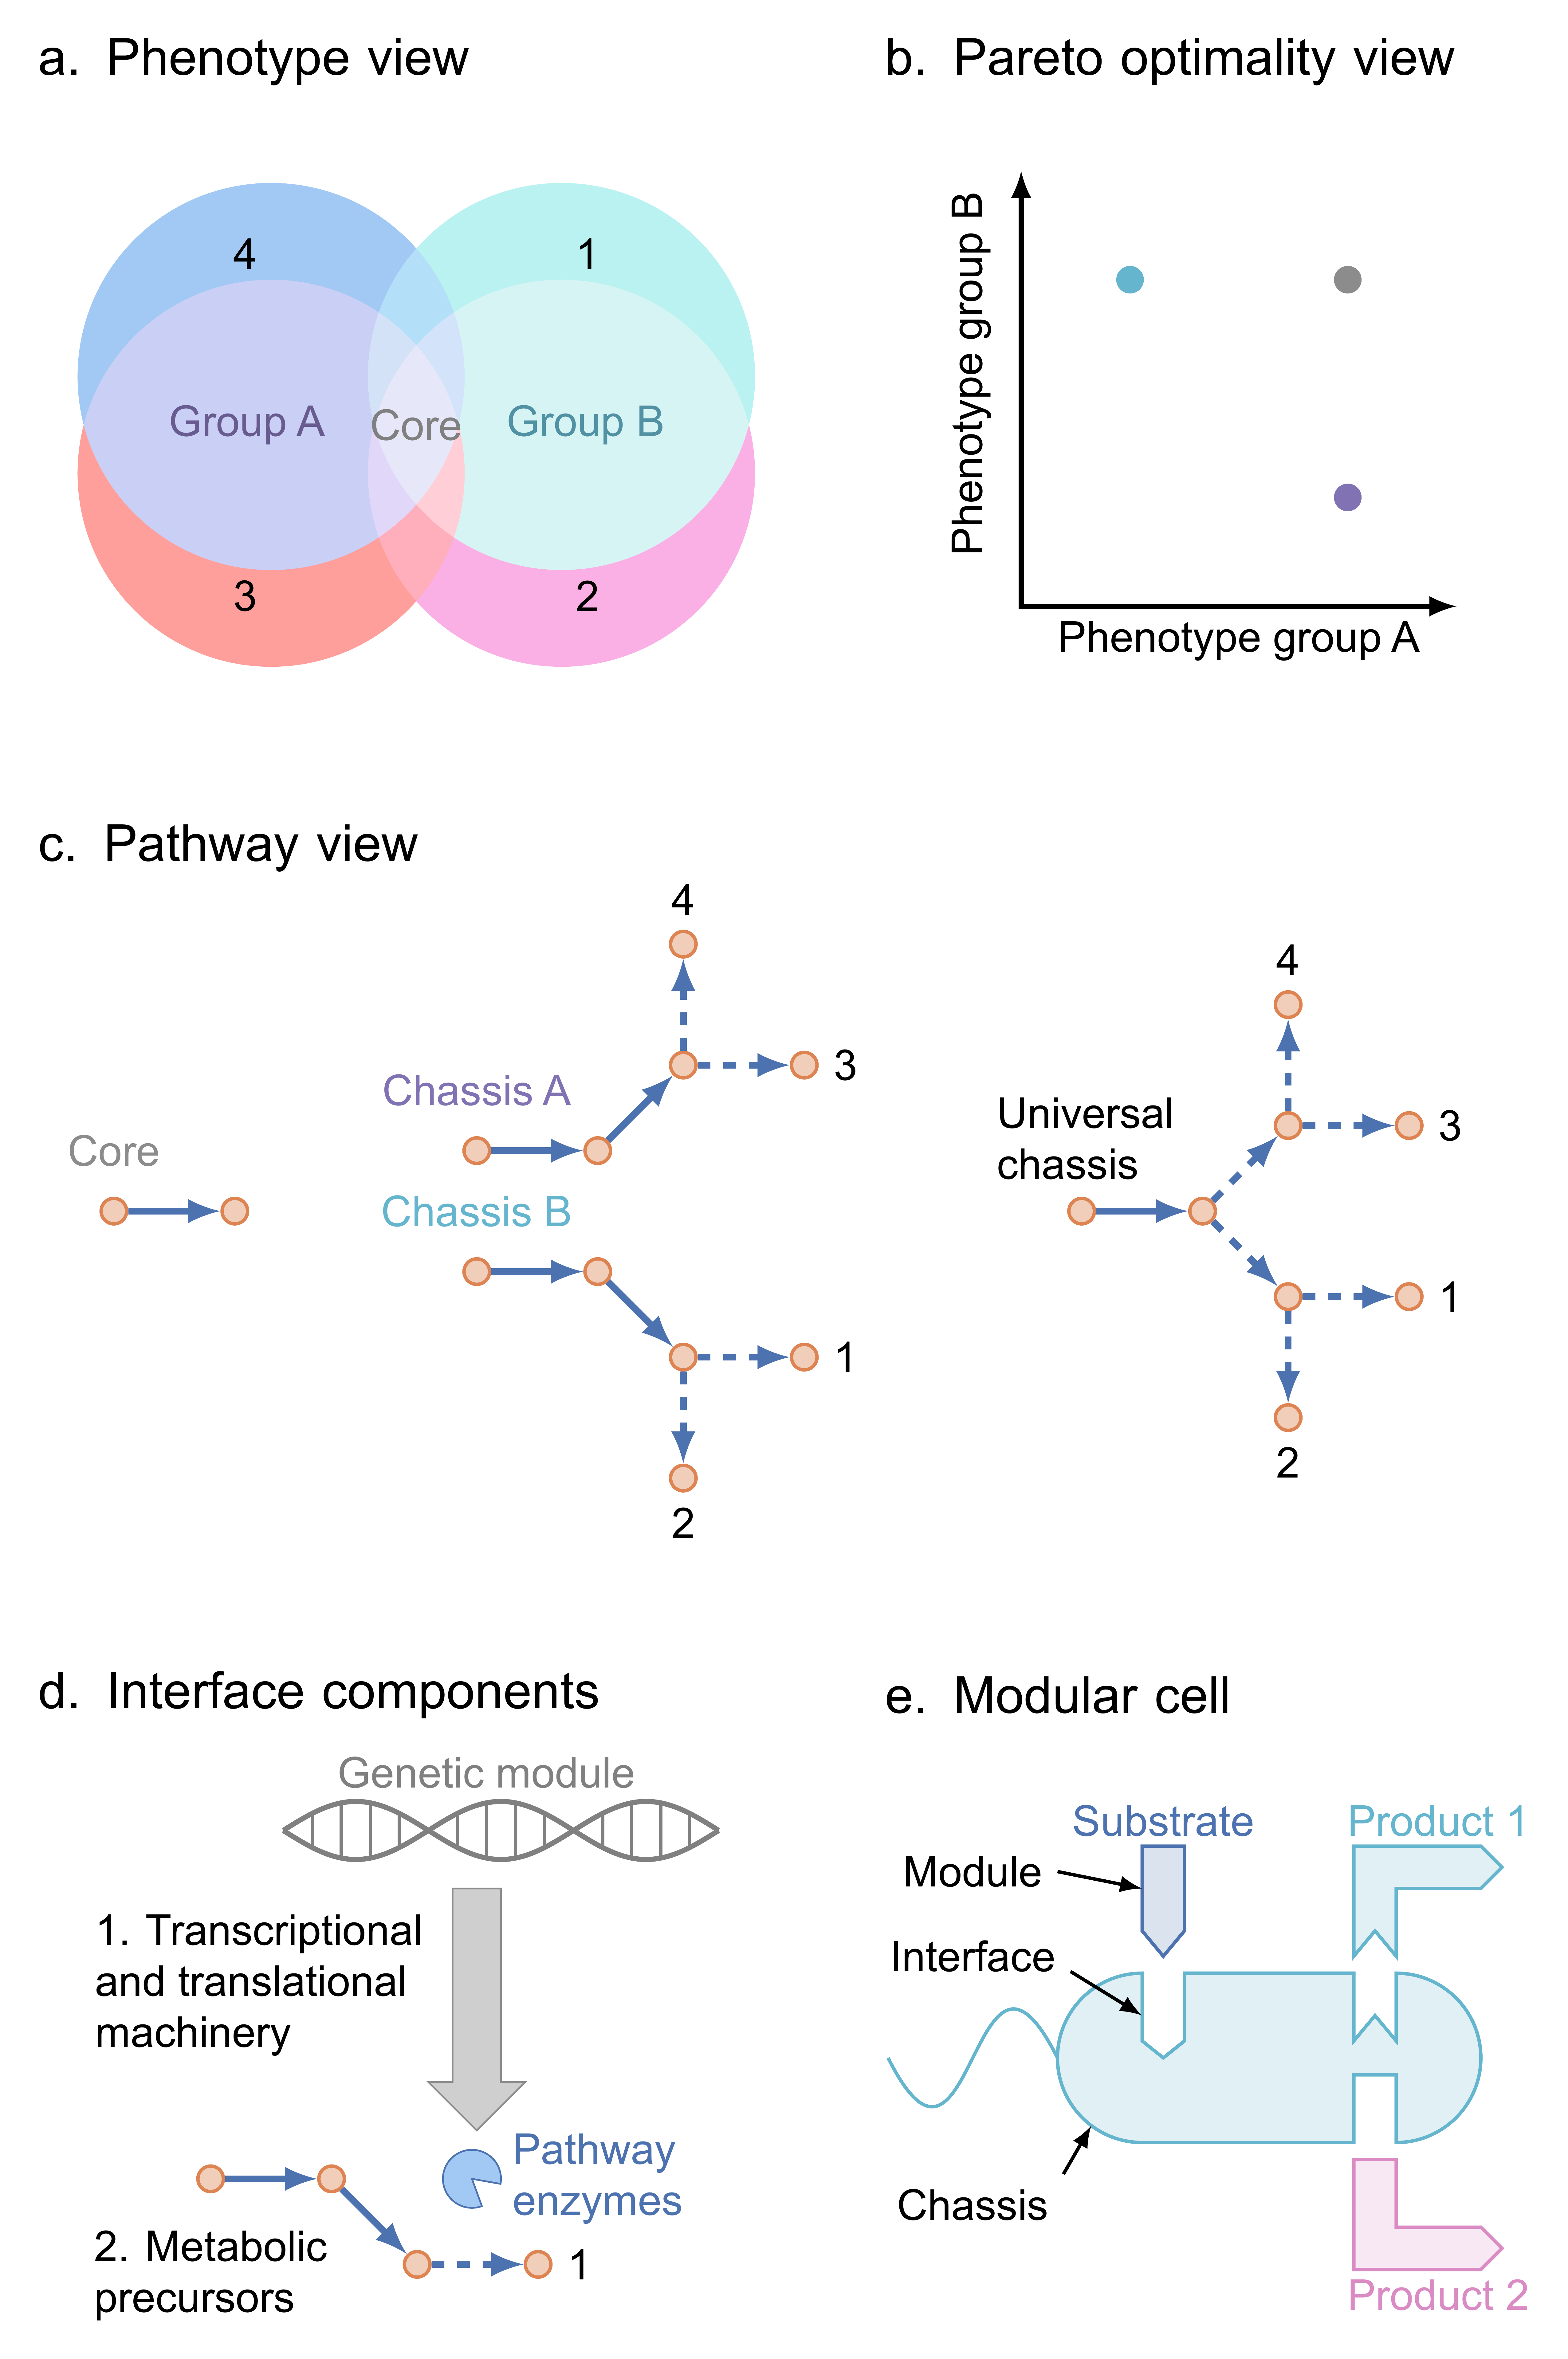
\includegraphics[height=.7\textheight,keepaspectratio]{modcell-concept.png}
    \caption[Modular cell design principles]{Modular cell design principles. (a) Multiple target phenotypes often share common functional states; e.g., different target molecules for overproduction that share precursors and undesired byproducts.
    (b) Several chassis strains are built by optimizing towards different phenotype groups, minimizing the effort required to build modules, at the expense of incompatibility among chassis. Alternatively, a universal core chassis can be build that would require more functions to be performed by the modules, likely introducing undesirable redundancy in module construction.
    (c) In the context of metabolic pathways, modularity can be described in terms of common precursors and downstream pathways.
    (d) The key component of a modular cell system are properly defined interfaces, the chassis must provide adequate enzyme biosynthesis machinery and metabolic precursors for modules to function properly. (e) The proposed modular cell is an efficient chassis strain compatible with modules that enable target phenotypes, minimizing redundant efforts and increasing robustness, hence accelerating the design-build-test cycles in strain engineering.
    }
    \label{fig7:modcell}
\end{figure}

%(Figure~\ref{fig7:modcell}a)
Engineering microbes towards novel phenotypes often repeats previous efforts leading to slower design cycles and less robust systems.
Alternatively, to avoid such redundancy we can design a modular cell chassis that interfaces with a variety of modules (Figure~\ref{fig7:modcell}).\citep{garcia2019, garcia2019b}
The modular cell chassis is built in a top-down manner by removing metabolic functions from a parent strain, then different modules are inserted into the chassis to obtain production strains that optimally display the target phenotype (e.g., high titer, rate, and yield of a given molecule).
Due to the conflicting biochemical requirements of different pathways %, under a limited number of genetic manipulations to construct chassis and modules,
the modular cell design problem was formulated as the following multi-objective optimization problem (MOP) known as ModCell2\citep{garcia2019}, which is summarized as follows:


\begin{alignat}{3}
    & \underset{ \; y_j, z_{jk}}{\max} \quad (f_1, f_2, \ldots, f_{|\mathcal{K}|})^T \quad \text{s.t.}  \label{eq7:of1} \\
    &  \quad f_k \in \, \text{arg }\underset{}{\text{max}} \Bigg\{ \frac{1}{f_k^{max}}\sum_{j \in \mathcal{J}_k} c_{jk}  v_{jk} \quad \text{s.t.} \label{eq7:of2}\\
    & \quad \qquad \sum_{j\in \mathcal{J}_k}S_{ijk}v_{jk} = 0 && \text{for all } i \in \mathcal{I}_k  \label{eq7:mb}\\
    & \quad \qquad  l_{jk} \le v_{jk} \le u_{jk}  && \text{for all } j \in \mathcal{J}_k \label{eq7:rb}\\
    & \quad \qquad  l_{jk} d_{jk} \le v_{jk} \le u_{jk} d_{jk} && \text{for all } j \in \mathcal{C} \label{eq7:db}\\
    & \quad \qquad \; d_{jk} = y_j \lor z_{jk} \; \Bigg\} && \text{for all } k \in \mathcal{K} \label{eq7:defdjk} \\
    & \quad z_{jk}\le (1-y_j) && \text{for all } j \in \mathcal{C}, \, k \in \mathcal{K} \label{eq7:mr1}\\
    & \quad \sum_{j \in \mathcal{C}}z_{jk} \le \beta && \text{for all } k \in \mathcal{K} \label{eq7:mr2} \\
    & \quad \sum_{j \in \mathcal{C}} (1-y_j) \le \alpha \label{eq7:a}
\end{alignat}

\noindent This MOP simultaneously maximizes all objectives $f_k$ \eqref{eq7:of1}, where $k$ belongs to the set of production networks $\mathcal{K}$.
Each production network represents the combination of the chassis with a specific production module, and it is simulated through a stoichiometric model\citep{palsson2015} (\ref{eq7:of2}-\ref{eq7:defdjk}) with a set of metabolites $\mathcal{I}_k$ and a set of reactions $\mathcal{J}_k$.
The stoichiometric model predicts metabolic fluxes according to the following constraints:
(i) mass-balance \eqref{eq7:mb}, where $S_{ijk}$ represents the stoichiometric coefficient of metabolite $i$ in reaction $j$ of production network $k$, (ii) flux bound \eqref{eq7:rb} that determine reaction reversibility and available substrates, where $l_{jk}$ and $u_{jk}$ are lower and upper bounds respectively, and (iii) genetic manipulation \eqref{eq7:db}, i.e., deletion of a reaction $j$ in the chassis through the binary indicator $y_{j}$, or insertion of a reaction $j$ in a specific production network $k$ through the binary indicator $z_{jk}$.
Only a subset of all metabolic reactions, $\mathcal{C}$, are considered as candidates for deletion, since many of the reactions in the metabolic model cannot be manipulated to enhance the target phenotype.

The desirable phenotype $f_k$ for production module $k$ is determined based on key metabolic fluxes $v_{jk}$ (mmol/gDCW/h) predicted by the model (\ref{eq7:of2}-\ref{eq7:db}).
For this study we selected the weak growth coupled to product formation (\emph{wGCP}) design objective that requires a high minimum product synthesis rate at the maximum growth-rate, enabling growth selection of optimal production strains.
Hence, in \emph{wGCP} design, the inner optimization problem seeks to maximize growth rate while calculating the minimum product synthesis rate through the linear objective function \eqref{eq7:of2} (where {$c_{jk}$ is $1$ and $-0.0001$ for $j$ corresponding to the biomass and product reactions across all networks $k$, respectively, and 0 otherwise).
In general, the definition of $f_k$ need not be linear and other design phenotypes can be defined.\citep{garcia2019}

Finally, design constraints (\ref{eq7:mr1}-\ref{eq7:a}) define the limitations of the design variables representing genetic manipulations, $y_j$ and $z_{jk}$.
As part of modular cell design, reactions can be removed from the chassis but inserted back to specific production modules, enabling the chassis to be compatible with a broader number of modules \eqref{eq7:mr1}.
The total module reaction additions and reaction deletions in the chassis are limited by parameters $\beta$ \eqref{eq7:mr2} and $\alpha$ \eqref{eq7:a}, respectively.%, to avoid unnecessary genetic manipulations that are generally time-consuming to implement and can lead to unforeseen phenotypes.


\subsection{Solution techniques for multi-objective optimization problem}
% All this info is background/lit reveiw, but it seems to fit better in its own section than in the intro
% - Define Pareto optimality
% - Explain why we choose MOEA instead of MILP? <= Is this a method?
% - Explain how MOEA works for next section (how important is this?)

Without loss of generality, consider a multi-objective optimization problem with design variables $x$ from a set $\mathcal{X}$ and objective functions $f_i(x)$:
\begin{equation*}
    \underset{ \;x}{\max} \quad F(x) = (f_1(x), f_2(x), \ldots)^T \; \forall x \in \mathcal{X}
\end{equation*}
The solution of such optimization problem is denoted as Pareto set:
\begin{equation*}
    \mathcal{PS}:=\{x \in \mathcal{X}:\nexists \, x' \in \mathcal{X}, F(x') \prec F(x)\} \label{eq7:ps}
\end{equation*}
Here $F(x') \prec F(x)$ indicates that the objective vector $F(x')$ \emph{dominates} $F(x)$, defined as $f_i(x') \ge f_i(x)$ for all objectives $i$, and $f_i(x') \ne f_i(x)$ for at least one $i$. Hence, the Pareto set contains all non-dominated solutions to the optimization problem, i.e., when comparing any two non-dominated solutions, the value of a certain objective must be diminished in order to increase the value of a different objective. The projection of the Pareto set on the objective space is denoted Pareto front: %This can be easily visualized in the Pareto front, defined as the projection of the Pareto set in the objective space: %TODO: Let the reader know why PF is useful? Since it is referenced later
\begin{equation*}
    \PF:=\{F(x): x \in \mathcal{PS} \}
\end{equation*}

MOP can be solved either directly or by conversion into a single-objective problem.\citep{marler2004}  When solved directly, multi-objective evolutionary algorithms (MOEA) are often used to identify the Pareto set, then the designer selects interesting solutions.
On the other hand, when the problem is converted into a single-objective optimization problem, this requires some form of \textit{a priori} specification of preference towards desired Pareto optimal points.
The main advantage of the second approach is that single-objective problems are easier to solve and powerful algorithms such as branch and bound used for mixed-integer linear programing (MILP) are available. % (Note: The state of the art solvers use also cutting planes and other heuristics on top of branch and bound. So I feel that branch and bound is not accurate enough  to later refer to it as the MILP solving method.)
Briefly, MOEA are population based heuristics where potential solutions are iteratively modified based on stochastic processes and information from other potential solutions to identify better solutions, while MILP solver algorithms systematically partition the design space to efficiently identify optimal solutions.
Both approaches have been successfully applied to design modular cells for problems with up to 20 objectives.\citep{garcia2019, garcia2019c, garcia2019d}
MILP can guarantee solution optimality, unlike MOEA. However, effective MILP solver algorithms remain highly challenging to parallelize. \citep{ralphs2016} % Also consider citing (can a million cores solve a ILP?)
Therefore, MOEA presents better options to address problems with many-objectives through high-performance computing as discussed next.

\subsection{Implementation of high-performance parallel many-objective evolutionary algorithm}
% - Describe master-slave vs island, why island is necessary, and other details that might be relevant in the implementation?
% - Define computing processes
% - The basics of genetic algorithms seem to have been introduced to late?
% - Explain any necessary background to understand the benchmarking results.
% - Important: Parameters need to be defined here to follow benchmarking discussion. Even easier, create a table that defines parameters.
% - Note MOEA are described above

The original ModCell2 implementation \citep{garcia2019, garcia2019c} is compatible with several MOEA and used a master-slave parallelization scheme, where the objective functions are evaluated in parallel by slave processes, but every other step in the algorithm is performed serially (Figure~\ref{fig7:algorithm}~a).
This approach contains many serial steps, limiting the scalability of the algorithm with the number processes according to Ahmdal's law.\citep{hill2008}
%In particular for one of the best performing algorithms NSGA-II time complexity \citep{garcia2019c}
In particular, large population sizes, an effective strategy to deal with many objectives,\citep{garcia2019c,ishibuchi2009} can dramatically slow down serial algorithm operations such as non-dominated sorting in NSGA-II, \citep{deb2002} one of the best performing algorithms to solve ModCell2.\citep{garcia2019c}%, quickly turning the serial part into a major performance bottleneck.


\begin{figure}[h]
    \centering
    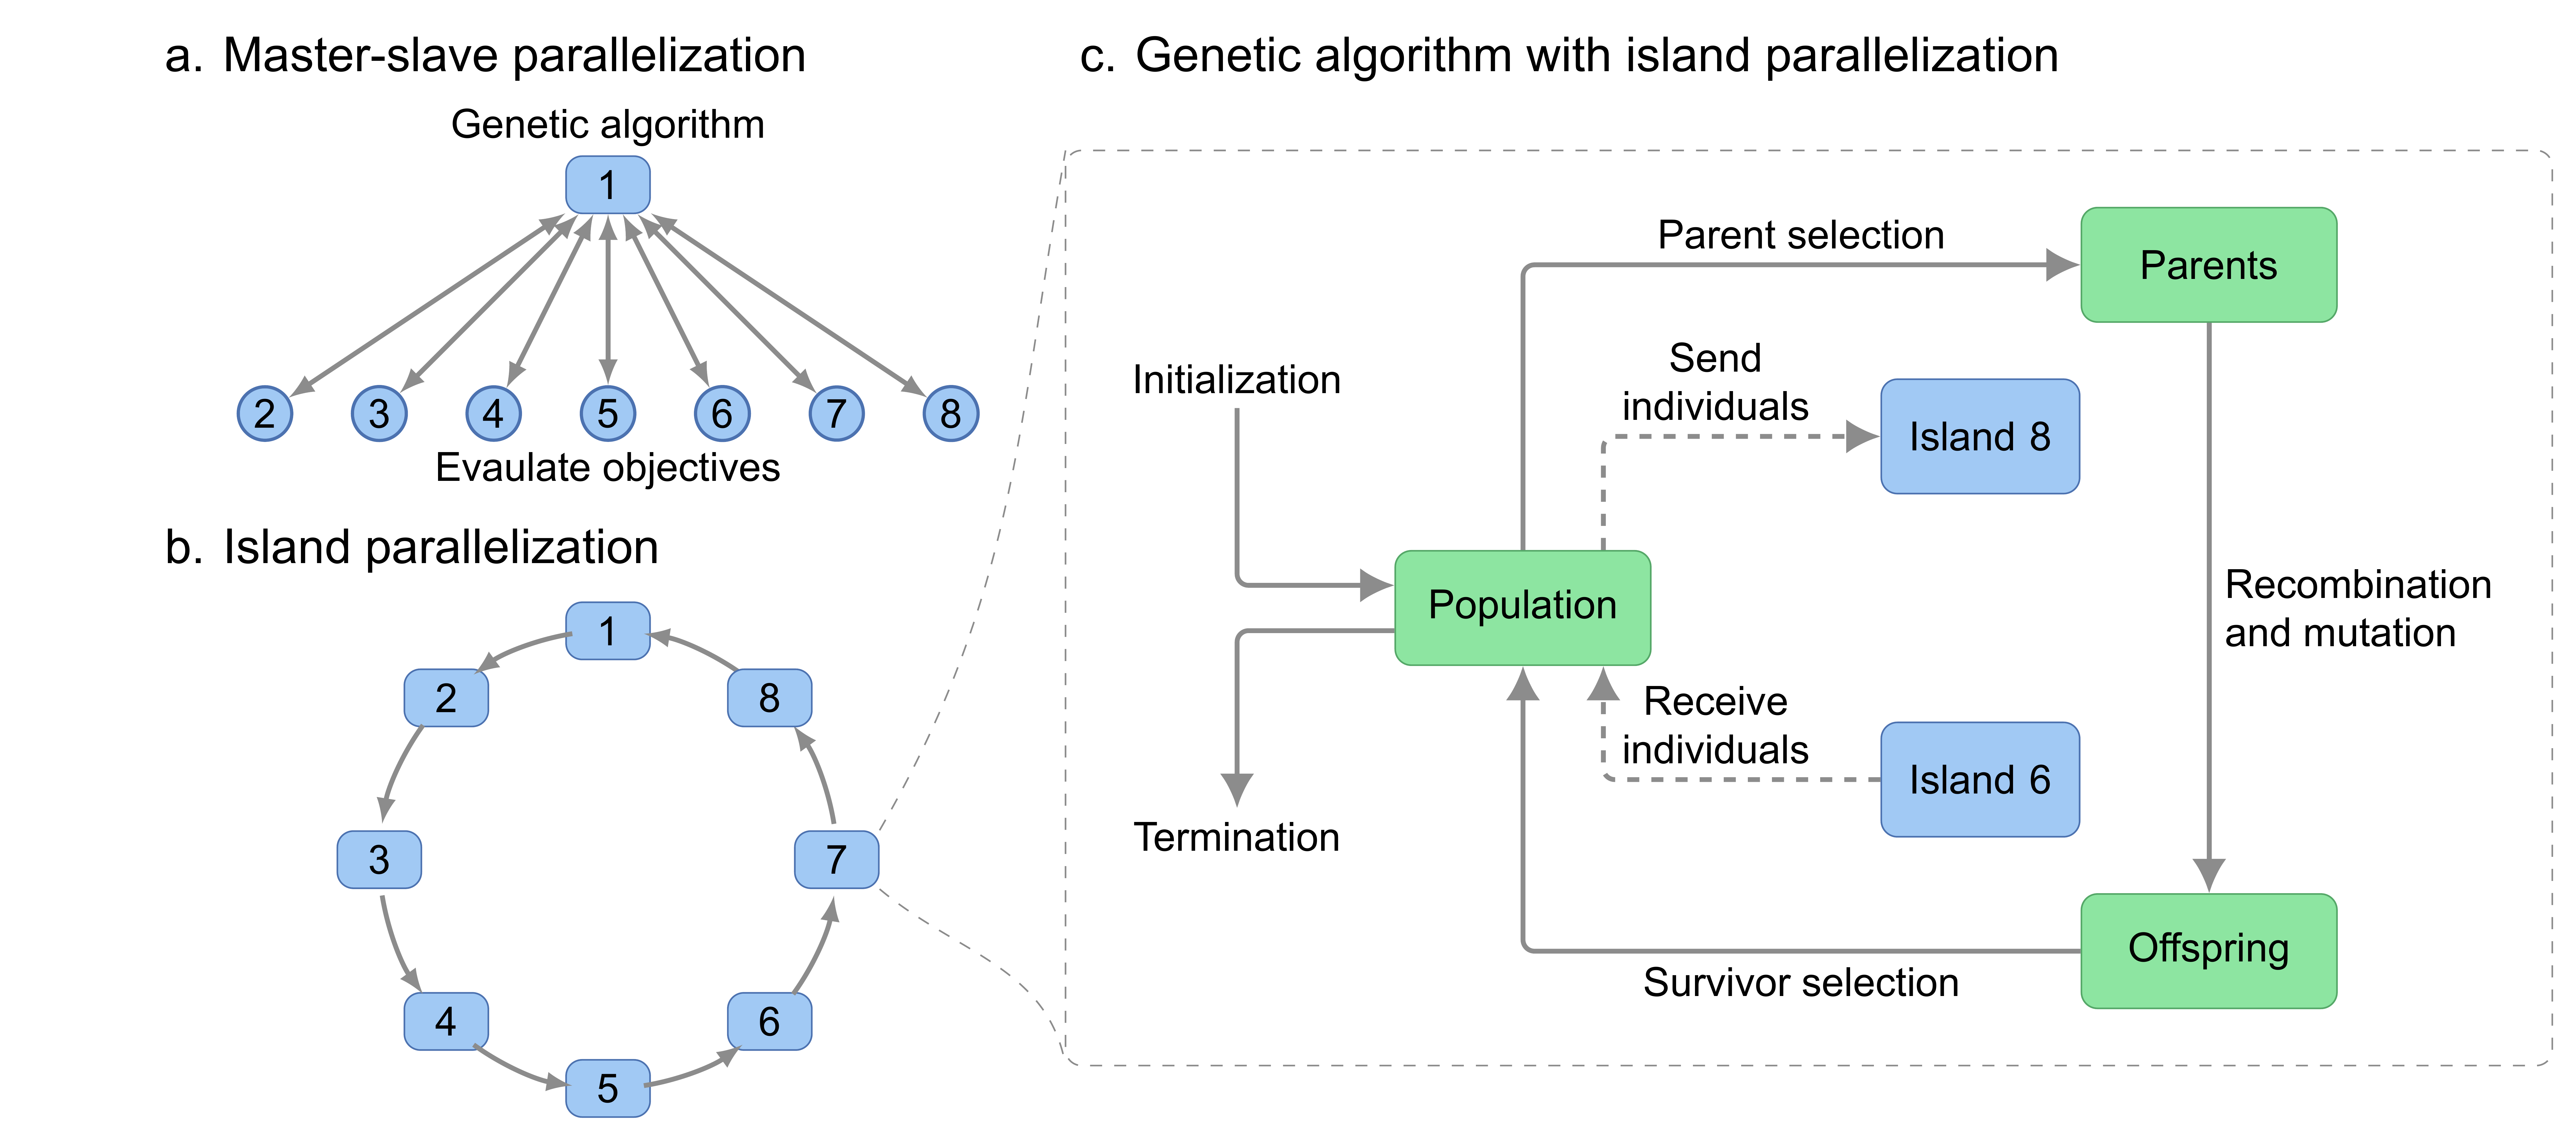
\includegraphics[width=\textwidth,keepaspectratio]{algorithm.png}
    \caption[Parallelization schemes for multi-objective evolutionary algorithm]{Parallelization schemes for multi-objective evolutionary algorithm. (a) Master-slave approach used in the original ModCell2 implementation. (b) Island parallelization following ring topology implemented in ModCell-HPC. (c) Key steps in evolutionary algorithm.} %TODO balance info here with text descritipon, but make the figure standalone. Provide brief ga description of part c, in particular describe the meaning of the words used in the figure.
    \label{fig7:algorithm}
\end{figure}

%An effective strategy to deal with many objectives is to use large
%In particular, for large populations sizes, an effective strategy to deal with large numbers of objectives, \citep{garcia2019c,ishibuchi2009},  certain algorithm steps like non-dominated population sorting in NSGA-II,\citep{deb2002} one of the best performing algorithms to solve ModCell2,\citep{garcia2019c}, quickly turning the serial part into a major performance bottleneck.

To overcome the issues of the master-slave approach, we implemented an island parallelization scheme, where each computing process is an instance of the MOEA (Figure~\ref{fig7:algorithm}~b).
These instances exchange individuals (i.e., potential solutions) in a process called migration, which enhances overall convergence towards optimal solutions (Figure~\ref{fig7:algorithm}~c).
The migration operation allows for multiple configurations that reflect which individuals are exchanged and how such exchange happens.
These options are captured by the migration type and migration interval parameters, respectively (Table~\ref{tab7:parameters}).
To enhance performance and scalability, the migration process was implemented asynchronously, i.e., the population within each island can continue to evolve without needing to wait for sent individuals to arrive at their destination island or for incoming individuals to be received.

The software implementation of the proposed island-MOEA, denoted \textit{ModCell-HPC}, is written from the bottom up in the C programming language and available in Supplementary~Material~\ref{sm:code} and \url{https://github.com/TrinhLab/modcell-hpc}.

%This migration process can occur in differentThe number of iterations in between migrations is denoted, \textit{migration frequency}
%A genetic algorithm is an iterative process where a population of potential solutions is modified under heuristic rules in order to identify solutions closer to optimality (Figure~\ref{fig7:algorithm}~c). In the island parallelization scheme, after a certain number of iterations, determined by the \textit{migration frequency}, individuals are sent and received to and from neighboring islands.
%(Table~\ref{tab7:parameters})

%In a genetic algorithm, a population composed by individuals that represent problem variables, is used to produce an offspring by stochastic combinations of their design variables and subsequent evaluation of their fitness (i.e., the design objectives of the optimization problem).


% \item The Matlab implementation of ModCell2 is slow and cannot handle large-scale problems due to both its inability to effectively parallelize beyond a few cores and its inefficient use of CPU and memory resources.
% \item modcell-hpc was written from the bottom up in C and uses MPI to implement island parallelization. In this approach multiple instances of the algorithm run in individual processes known as islands. These islands exchange individuals with certain periodicity in a process called migration.
% \item Migration occurs asynchronously so islands may continue to evolve while messages are being passed, greatly enhancing performance.
% \item This approach can potentially scale to hundredths or thousands of cores since the program does not contain any sequential operations that would become a bottleneck (See Amdahl's Law).

\subsection{Computation hardware}
We conducted all ModCell-HPC computations in \emph{beacon} nodes from the Advanced Computing Facility at the Joint Institute for Computational Science (The University of Tennessee and Oak Ridge National Laboratory). Each node contains a 16 core Intel Xeon E5-2670 central processing unit (CPU) and 256 GB of random access memory (RAM). The results were analyzed in a desktop computer with an Intel Core i7-3770 CPU and 32 GB of RAM.

\subsection{Target product identification}
The target products are endogenous \textit{E. coli} metabolites that meet the following requirements: i) Maximum theoretical yield above 0.1 (mol product/mol of substrate); ii) organic; iii) can be coupled to growth under anaerobic conditions, indicated by the existence of a constrained Minimal Cut Set (cMCS) with yield above 50\% under anaerobic conditions in a previous study;\citep{kamp2017} iv) If the same metabolite appears in multiple compartments, only one instance is selected, prioritizing extracellular, then periplasm, then cytosol.
This resulted in 161 target metabolites.
Metabolites that did not have a secretion mechanism originally present in the model required to add an exchange pseudo-reaction that represents metabolite secretion to the growth medium or intracellular accumulation at steady-state. %TODO: Not sure where to mention this, or if very relevant at all.
The products in the resulting library have diverse molecular weights and are highly reduced due to the use of anaerobic conditions (Figure~\ref{fig7:biochemical-properties}).

%If the same metabolite

% Either explain in the table or on the text but avoid redundancy
%The target products are endogenous \textit{E. coli} metabolites that have the potential to be produced in a growth-couple manner according to a previous study by Kamp and Klamt.\citep{kamp2017}
%We further filtered the target products according to the criteria of Table \ref{tab7:products}.
%In summary, only endogenous metabolites that are organic, have a maximum theoretical yield above 0.1 (mol product / mol of substrate) and can potentially be coupled to growth under anaerobic conditions were kept as targets.

\subsection{Model configuration}
Since the study of Kamp and Klamt\citep{kamp2017} was used as basis to identify products compatible with growth-coupled design, we used the same model configuration, adapted to the most recent \textit{E. coli} model iML1515.\citep{monk2017} Briefly, glucose uptake limit was set to 15 (mmol/gCDW/h); the default ATP maintenance value in iML1515 was used; 20\% of the maximum anaerobic growth rate was used as the minimum growth rate, corresponding to 0.0532 (1/h). The model configuration is equivalent to previous modular cell design studies\citep{garcia2019} except for the higher glucose uptake rate.

%The only difference between anaerobic and aerobic model configurations is the oxygen uptake rate limit, which is 0 in the former and 20 mmol/gCDW/h in the later.

\subsection{Solution improvement process}
The MOEA output can be improved by: i) eliminating \emph{futile module reactions}, i.e., module reactions that when removed do not diminish the objective value of the associated production network; and ii) coalescing module reaction, i.e., in multiple designs with the same deletions, but different module reactions, can often be combined to obtain a superior solution. This procedure is detailed in Figure~\ref{fig7:processing}.
%We applied this improvement process to anerobic and aerobic results and observed remarkable improvement in solution quality. (most module reactions are futile, the PF of $\alpha=5,\beta=1$ has a minimal set cover of 8 before coalescing and 3 after coalescing.
% NOTE: This was not applied to benchmarking, but was applied to all other solutions.

\subsection{Design characterization} \label{sec:design_characterization}
\subsubsection{Compatible modules and compatibility}
An important qualitative feature of a designed chassis is module compatibility.
A chassis and a given module are \emph{compatible} if the performance of such module is above a defined threshold.
In this study, we used the \textit{wGCP} design objective that corresponds to the minimum product yield at the maximum growth rate, and selected a threshold of 0.5 to establish compatibility. Under these conditions, we expect a module compatible with the chassis can lead to a product yield above 50\% of the theoretical maximum during the growth phase.
The \emph{compatibility} of a chassis corresponds to the number of modules that are compatible with it.

\subsubsection{Minimal covers} \label{sec:minimal_covers}
After solving the modular cell  design problem, we obtain several Pareto optimal chassis, $h \in \mathcal{H}$, that are compatible with different subsets of products. %I.e., a design $h$ is said to be compatible with product $k$, if its objective function is above a defined threshold.
A set cover is a collection of designs $h$ such that their union contains all compatible products.
Hence, we developed minimal set cover analysis to find the smallest number of designs needed to ensure all compatible products are present in at least one of the designs.
This is formulated as the canonical minimal set covering problem of integer programming:

\begin{align}
    & \underset{ \;x_h \in \{0,1\}}{\min} \sum_{h \in \mathcal{H}} ( \gamma_h x_h) \label{eq7:mc_1}\\
    & \nonumber \; \text{subject to:} \\
    & \quad \sum_{h \in \mathcal{H}} a_{hk} x_h \ge 1 & \forall \; k \in \mathcal{K'} \label{eq7:mc_2}%\\
    %& \quad x_h \in \{0,1\} & \forall h \in \mathcal{H} \label{eq7:mc_3}
\end{align}

\noindent
The optimization problem minimizes the number of designs in the set cover \eqref{eq7:mc_1}.
The binary indicator variable $x_h$ takes a value of 1 if design $h$ is selected as part of the cover and 0 otherwise.
Certain designs can be prioritized (e.g., due to the genetic manipulations they contain being preferable or to reduce the number of alternative solutions) using the weighting parameter $\gamma_h$, however in all our simulations we set $\gamma_h = 1$. All compatible products $k$ must be included in at least one of the selected designs \eqref{eq7:mc_2}. The parameter $a_{hk}$ takes a value of 1 if product $k$ is compatible with design $h$ and 0 otherwise. There must exist at least one $h \in \mathcal{H}$ for which $a_{hk} = 1$ to ensure a feasible solution exists, hence $\mathcal{K'}$ is the set of products compatible in at least one design of the Pareto front.
%Thus if a product is not compatible at all under the specified modcell design parameters ($\alpha$ and $\beta$) it must be discarded from $\mathcal{K'}$ or the problem would become infeasible.

To enumerate all minimal covers we iteratively solved the minimal cover problem (\ref{eq7:mc_1}-\ref{eq7:mc_2}) with the addition of an integer cut inequality \eqref{eq7:ic} in each iteration that removes a previously found solution $\mathcal{S}$.
\begin{equation}
    \sum_{h\in\mathcal{S}} x_h \le |\mathcal{S}|  - 1 \label{eq7:ic}
\end{equation}
%Here $\mathcal{S}$ is a previously found optimal solution that should be excluded from the problem.


\section{Results}

\subsection{Design of modular \textit{E. coli} platform strains for growth-coupled production}

\paragraph{A small number of genetic manipulations are sufficient for highly compatible chassis}
We tuned ModCell-HPC method parameters (Supplementary Text 1) and used it to design \textit{E. coli} modular cells for our library of 161 products.
%, we used ModCell-HPC to design modular cells.
First, we scanned a broad range of design parameter combinations ($\alpha$-$\beta$: 5-1, 10-2, 20-4, and 40-8) to identify the required genetic manipulations for highly compatible designs (Figure~\ref{fig7:parameter-scan} a).
Increasing the number of genetic manipulations leads to an average increase in design compatibility.
However, the maximum compatibility remains around 50\% of the library (80 products) for all cases.
Indicating that highly compatible platforms can be built with a small number of genetic manipulations.
We selected the designs with case of $\alpha=5,\beta=1$ (Supplementary~Material~\ref{sm:designs}) for further analysis, since designs with fewer genetic manipulations are likely more accurately simulated and also easier to implement in practice.
%We will analyzed overall features of the designs , then focus on specific suggestions for experimental implementation.

\paragraph{A few reaction deletions in central metabolism targeting byproducts and branch-points are relevant to build chassis strains}
% Key points:
% - Few reactions are relevant
% - Reactions are concentrated in central metabolism
% - Reactions belong to two categories: Remove undesired byproducts and metabolic branchpoints
% - Branchpoitns are not commonly targeted, even though their potential importance was highlighted early on:
% https://science.sciencemag.org/content/252/5013/1675
% \citep{stephanopoulos1991}
% the use of models may assist in solving the problem

We sorted reaction deletions according to how often they appear across designs (Table~\ref{tab7:top20deletions}).
The top 7 reactions are used $\ge$10\% of the designs and belong to central metabolism, indicating their importance to accomplish growth coupled to product secretion phenotypes.
%The top 20 reactions mainly belong to central metabolism (Figure~\ref{fig7:deletion-map}), and quickly decay in deletion frequency, highlighting the relevance of the top 3 reactions, appearing in >40\% of the designs, to accomplish the target growth coupled to product secretion phenotypes.
% Central metabolism:
% sauer1999
%The top 3 deletions all apear in 40\% or more of the designs.
%However, this frequency quickly decays.
%Indicating that these reactions, ALCD2x, TPI, and ACALD, are key deletions for growth-coupled product synthesis.
%Both ALCD2x and ACALD are involved in the conversion of acetyl-CoA to ethanol, which is the main pathway for acetyl-CoA reduction and secretion under anaerobic conditions. Unsuprisingly this pathway must be avoided to couple target molecule secretion to growth.
Overall, the role of these deletions can be classified into two functions: i) To eliminate major byproducts; ii) to alter key branch-points in metabolism that influence the pools of precursor metabolites (including carbon, redox, and energy precursors).
% and overall energy efficiency of catabolism.
The first type is generally intuitive and often used in metabolic engineering efforts.\citep{winkler2015}
The second type are not commonly identified unless metabolic model simulations are used, \citep{tokuyama2014, venayak2018, chemler2010}
even though the importance of targeting metabolic branch-points was noted early. \citep{stephanopoulos1991}
%importance of manipulating key metabolic branch-points that are not part or directly upstream of the production pathway was noted early.\citep{stephanopoulos1991}
% - Branchpoitns are not commonly targeted, even though their potential importance was highlighted early on:
% \citep{stephanopoulos1991}
Examples of the later manipulations are TPI deletion, that activates the methylglyoxal bypass,\citep{fong2006} reducing the overall ATP yield resulting from glucose conversion into pyruvate.
Lower ATP yield limits biomass formation hence redirecting carbon flow towards products of interest.
While such strategies are not common, TPI deletion predicted by model simulations was successfully used for enhanced 3-hydroxypropionic acid production,\citep{tokuyama2014} and ATP waisting is receiving increased attention to enhance production of certain molecules.\citep{boecker2019} %NOTE: MAybe ATP waistin is a bit of a strech here?
Another example of branch-point manipulation is PPC deletion, that has been shown to lower flux from lower glycolysis towards the TCA cycle,\citep{de2006,peng2004} resulting in lower succinate production, and an increased pool of \textit{pep}, pyruvate and acetyl-CoA.
Additionally, PPC deletion to increase the \textit{nadph} pool for production of flavonoids was predicted by model simulation and experimentally validated. \citep{chemler2010}
%which synthesis important precursors and also enables succinate secretion. %\citep{} %see MILP paper for succinate citations
In summary, design of highly compatible chassis strains requires not only major byproduct removal, but also manipulation of key branch points in central metabolism.

\begin{table}[ht]
    \caption[Top 20 reaction deletions]{Top 20 reaction deletions for design parameters $\alpha=5$, $\beta=1$ with 162 designs. Counts indicates the percentage of designs where the deletion is used. All reaction and metabolite abbreviations used in this study correspond to BiGG identifiers (\protect\url{http://bigg.ucsd.edu}).}
    \centering
    \resizebox{1\textwidth}{!}{%
\rowcolors{2}{gray!25}{white}
\begin{tabular}{llll}
\toprule
ID	&	Name	&	Formula	&	Counts (\%) \\
\midrule
ALCD2x	&	Alcohol dehydrogenase (ethanol)	&	etoh\_c + nad\_c $\leftrightarrow$ acald\_c + h\_c + nadh\_c	&	57.4	\\
TPI	&	Triose-phosphate isomerase	&	dhap\_c $\leftrightarrow$ g3p\_c	&	45.1	\\
ACALD	&	Acetaldehyde dehydrogenase (acetylating)	&	acald\_c + coa\_c + nad\_c $\leftrightarrow$ accoa\_c + h\_c + nadh\_c	&	40.7	\\
FLDR2	&	Flavodoxin reductase (NADPH)	&	2.0 flxso\_c + nadph\_c $\rightarrow$ 2.0 flxr\_c + h\_c + nadp\_c	&	24.1	\\
PPC	&	Phosphoenolpyruvate carboxylase	&	co2\_c + h2o\_c + pep\_c $\rightarrow$ h\_c + oaa\_c + pi\_c	&	21.6	\\
TKT2	&	Transketolase	&	e4p\_c + xu5p\_\_D\_c $\leftrightarrow$ f6p\_c + g3p\_c	&	15.4	\\
LDH\_D	&	D-lactate dehydrogenase	&	lac\_\_D\_c + nad\_c $\leftrightarrow$ h\_c + nadh\_c + pyr\_c	&	13	\\
G3PD2	&	Glycerol-3-phosphate dehydrogenase (NADP)	&	glyc3p\_c + nadp\_c $\leftrightarrow$ dhap\_c + h\_c + nadph\_c	&	7.4	\\
POR5	&	Pyruvate synthase	&	coa\_c + 2.0 flxso\_c + pyr\_c $\leftrightarrow$ accoa\_c + co2\_c + 2.0 flxr\_c + h\_c	&	7.4	\\
ACKr	&	Acetate kinase	&	ac\_c + atp\_c $\leftrightarrow$ actp\_c + adp\_c	&	6.8	\\
THD2pp	&	NAD(P) transhydrogenase (periplasm)	&	2.0 h\_p + nadh\_c + nadp\_c $\rightarrow$ 2.0 h\_c + nad\_c + nadph\_c	&	6.2	\\
GLUDy	&	Glutamate dehydrogenase (NADP)	&	glu\_\_L\_c + h2o\_c + nadp\_c $\leftrightarrow$ akg\_c + h\_c + nadph\_c + nh4\_c	&	5.6	\\
ASPT	&	L-aspartase	&	asp\_\_L\_c $\rightarrow$ fum\_c + nh4\_c	&	5.6	\\
ASNS2	&	Asparagine synthetase	&	asp\_\_L\_c + atp\_c + nh4\_c $\rightarrow$ amp\_c + asn\_\_L\_c + h\_c + ppi\_c	&	4.9	\\
CBMKr	&	Carbamate kinase	&	atp\_c + co2\_c + nh4\_c $\leftrightarrow$ adp\_c + cbp\_c + 2.0 h\_c	&	4.3	\\
RNDR4	&	Ribonucleoside-diphosphate reductase (UDP)	&	trdrd\_c + udp\_c $\rightarrow$ dudp\_c + h2o\_c + trdox\_c	&	3.7	\\
RPE	&	Ribulose 5-phosphate 3-epimerase	&	ru5p\_\_D\_c $\leftrightarrow$ xu5p\_\_D\_c	&	3.1	\\
SERD\_L	&	L-serine deaminase	&	ser\_\_L\_c $\rightarrow$ nh4\_c + pyr\_c	&	3.1	\\
LCARS	&	Lacaldehyde reductase (S-propane-1,2-diol forming)	&	h\_c + lald\_\_L\_c + nadh\_c $\leftrightarrow$ 12ppd\_\_S\_c + nad\_c	&	2.5	\\
FUM	&	Fumarase	&	fum\_c + h2o\_c $\leftrightarrow$ mal\_\_L\_c	&	2.5\\
\hline
\end{tabular}}

    \label{tab7:top20deletions}
\end{table}

%PPC
%TKT2
% TKT1 overxpression is imnportant for aromatic aminoacids and other products

% This paper as ppc and tpi deletion, though just examined in the context of evolution:
% https://www.nature.com/articles/ng1432

%Notably the actitivty of this gene, w.... evolved mutants. Highlighting that special care must be t... for underground metabolism in growth-coupled design % \citep{wilbanks2017}


% Note above flavodoxin dependent
% https://ecocyc.org/ECOLI/NEW-IMAGE?type=ENZYME&object=Flavodoxin
%  These are not commonly paid attention in e.coli, even though they are known to be active (when?). No clear reason why
% In terms of the model FLDR2 for example exchange nadph and fldx then POR5 can oxidize pyruvate using nadph

\paragraph{Module reaction usage reveals pathway interfaces and unbiased module definition}
% Key points:
% - Reminder of module reactions, enhance compatibility
% - We can identify what reactions are critical for certain producst
% - Instead of defining what reactions must be present in a module, this allows to ... Further flux analysis as done previously can also lead to reactions that should be overexpressed.
% - Use the trivial cases first (e.g., acetate, lactate, ethanol) then move on to the more sophisticated pathways/less obvious cases.
The modular cell optimization formulation not only identifies genetic manipulations in the chassis, but also in the production modules.
Module reactions correspond to reactions deleted in the chassis but inserted back in specific production modules to enable compatibility.
We examined the module reactions used by all designs (Figure~\ref{fig7:module-usage}).
As expected, ethanol often uses ALCD2x, acetate uses ACKr, and lactate LDH\_D, all these are the primary producers of those metabolites.
More notably, we observe that products which are not highly reduced such as acetate, use ACALD, and similarly 3-methyl-2-oxobutanotae and 2,3-dihydroxy-3-methylbutanoate (which are naturally precursors of valine and artificially of isobutanol\citep{atsumi2008,atsumi2010}) use FUM and MDH.
These module reactions enable the synthesis of ethanol and succinate, respectively, necessary to maintain electron balance in the production of less reduced metabolites.
Interestingly, fatty acids tend to use TPI, which as mentioned earlier, its deletion activates the methylglyoxal bypass lowering the overall ATP yield.
The first step in fatty acid biosynthesis, acetyl-CoA carboxylase, requires one ATP per mol of malonyl-CoA, explaining the usage of TPI as a module reaction for this family of products.
Overall, module reactions provide with a systematic method to enhance the compatibility of a chassis, leading to more efficient strategies and revealing potential metabolic flux bottlenecks that are not always directly upstream of the target product.


\begin{figure}[h]
    \centering
    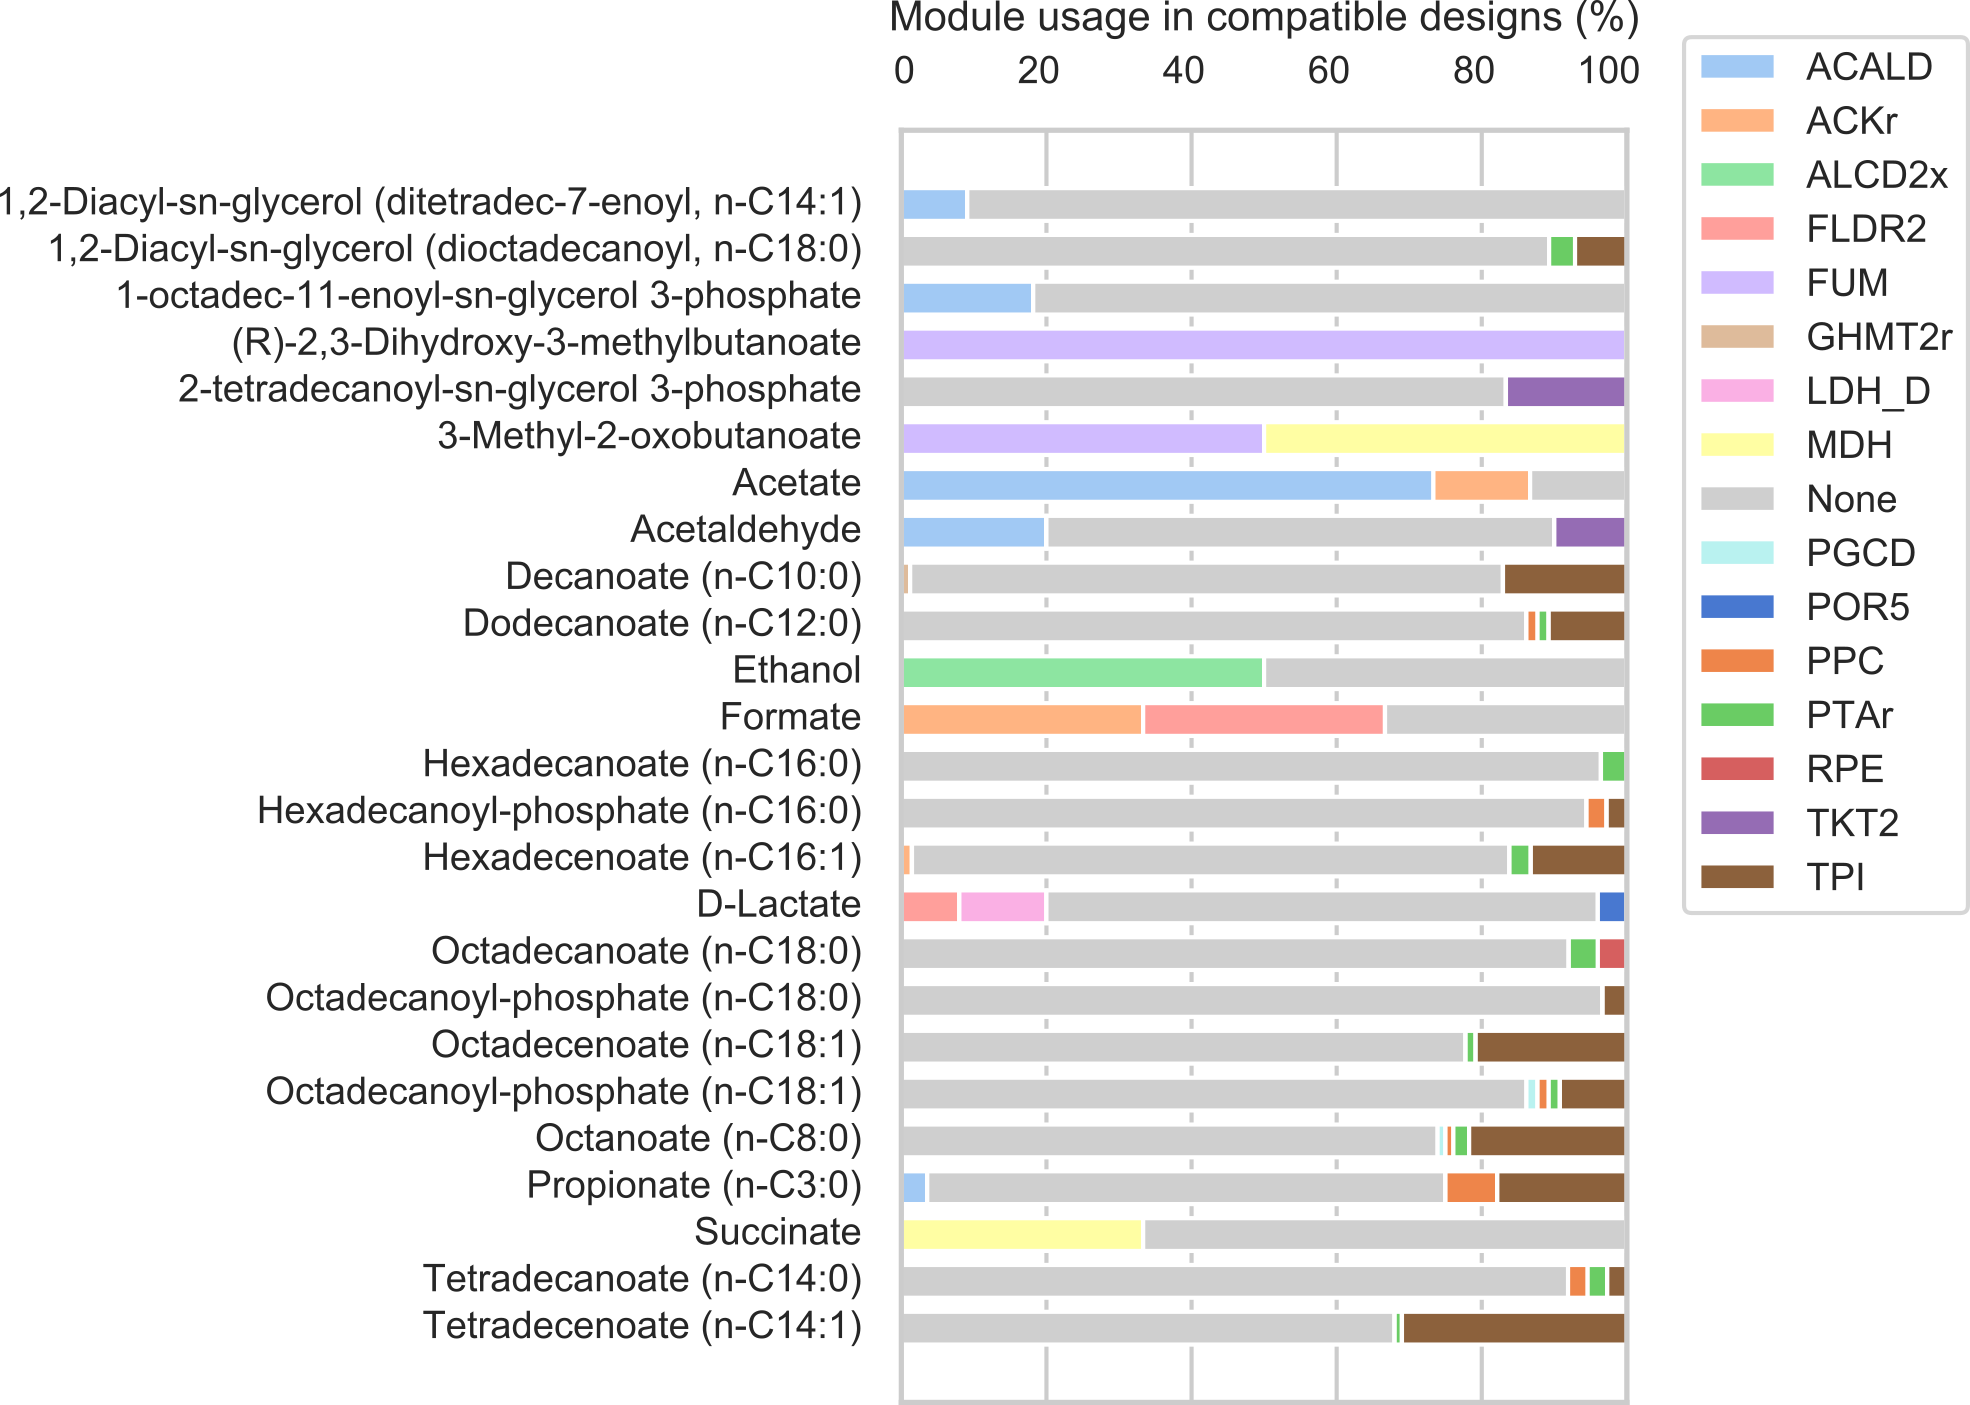
\includegraphics[width=\textwidth,keepaspectratio]{a5_b1_comp_0p5_module_usage.png}
    \caption[Module reaction usage]{Module reaction usage for design parameters $\alpha=5$ and $\beta=1$. Only designs compatible with the product are considered in the module usage frequency.}%For each product, designs in which the product is compatible are selected and the frequency of used module reactions is extracted.}
    \label{fig7:module-usage}
\end{figure}

% Why not many products use module reactions?

\paragraph{Three chassis strains is the smallest set of designs needed to cover all compatible modules}
% Key points:
% - We apply minimal covers to demonstrat the smallest ...
% - We find in this case the minimal cover size is 3, there are xxx, resulting form
One of the tenets of efficient design is to minimize redundant efforts.
When it comes to the construction of platform strains, we would like to identify the smallest set of strains needed to cover a certain product library.  %while avoiding redundancy.
To address this question we use the set of designs produced by ModCell-HPC and a set covering optimization problem (Section~\ref{sec:minimal_covers}).
%We applied this analysis to the set of designs with
For the Pareto set of designs $\alpha=5,\,\beta=1$ we  enumerated a total of 12 minimal covers of size 3. These covers are spanned by combinations of 8 unique designs (Figure~\ref{fig7:cover-graph}). %NOTE: Could add the table with designs
We selected cover k that contains designs 82, 121, and 124, which use few deletions and have similar genetic manipulations among them.
All designs in the cover have in common the deletion of ALCD2x and LDH\_D, disabling production of ethanol and lactate, the major reduced products of anaerobic growth in \textit{E. coli}.
% and well-known targets.
Designs 121 and 124 are compatible with the same 57 products, and design 121 is uniquely compatible with ethanol, formate, and 2,3-dihydroxymethylbutanoate, while design 124 is uniquely compatible succinate (Figure~\ref{fig7:design-comparison} a).
These two designs only differ in that design 121 uses FUM deletion while design 124 uses MDH deletion,
(Figure~\ref{fig7:design-comparison} b)
FUM deletion blocks metabolic flux towards succinate secretion%
%FIXME: this can be contradictory with what I said earlyr about 23dhmb production,
, while MDH routes it toward this product (Figure~\ref{fig7:design-comparison} c).
%Given a few additional genetic manipulations they could potentially be combined. % NOTE: Probably not good to say, since someone might suggest to do it
Design 82 is the only design that features the deletion of FLDR2 and PPC, and it is uniquely compatible with 24 modules, all fatty acids, making this design quite different from from 121 and 124.
FLDR2 is coupled with POR5 to form a pathway for the reduction of pyruvate into acetyl-coa consuming \textit{nadph} (Figure~\ref{fig7:design-comparison} c), a key redox cofactor in fatty acid biosynthesis.
PPC deletion is another strategy to increase \textit{nadph} available that has been experimentally validated. \citep{chemler2010}
Overall, these designs can be efficiently built due to their similarity,  and are composed of strategies that have been demonstrated in isolation but also seem applicable to cover large product families.

\begin{figure}[hp]
    \centering
    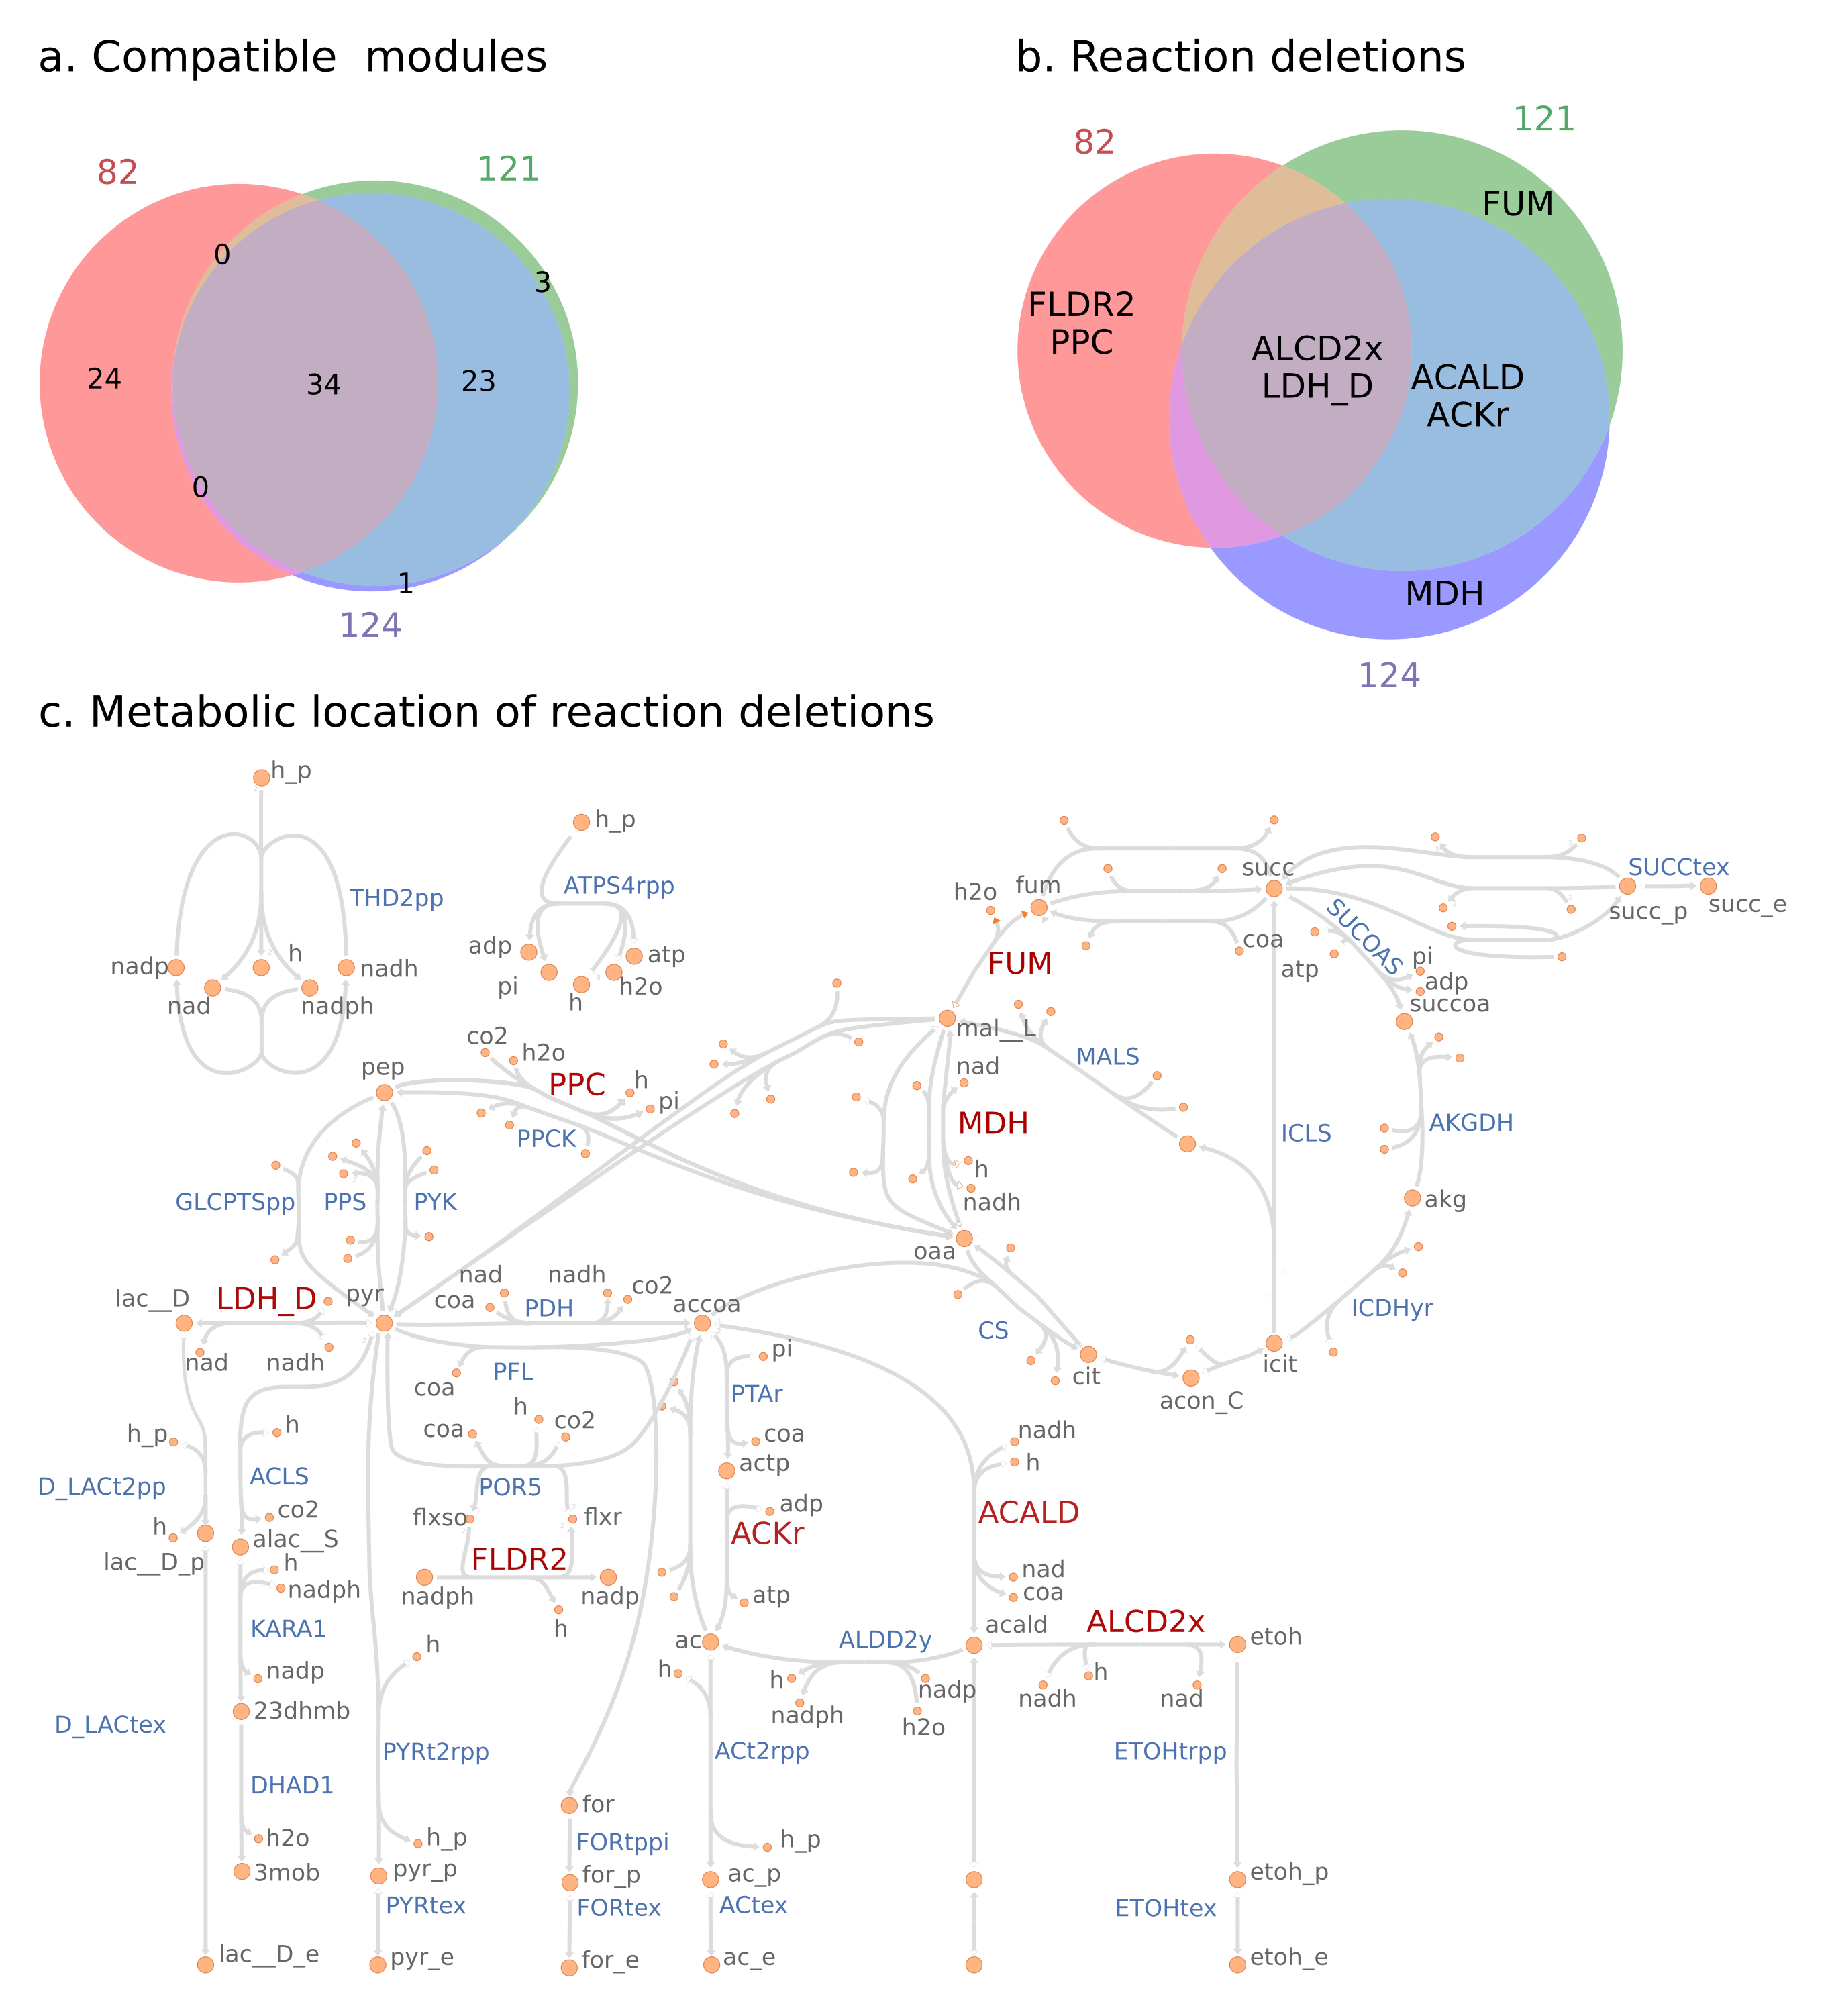
\includegraphics[width=\textwidth,keepaspectratio]{cover-venns.png}
    \caption[Comparison of designs in the selected minimal cover]{Comparison of designs in the selected minimal cover. (a) Venn diagram of products compatible with each design. The products uniquely compatible with specific designs are:
       Design 121: \textit{etoh, for, 23dhmb};
       Design 124: \textit{succ};
%       Design 25: \textit{pe120, 2agpg180, 1ddecg3p, 1agpg180, pgp140, pgp120, pg141, pg140, 2odecg3p, pgp141, ps140, lipidX, 2tdecg3p, ps141, pg120, pe140, 2odec11eg3p, pe141, apg120, ps120, 2hdecg3p, 2hdec9eg3p, pgp161, pg161}.
       Design 82: \textit{pg140, 2hdecg3p, 2odec11eg3p, 1agpg180, pe140, pg161, pg141, 2hdec9eg3p, pgp161, 2agpg180, 1ddecg3p, pg120, pgp141, pgp140, pe141, ps140, apg120, ps120, pgp120, pe120, lipidX, 2tdecg3p, 2odecg3p, ps141}.
    (b) Venn diagram of reaction deletions that constitute each design.
    (c) Metabolic map with reaction deletions colored in red.
       }
    \label{fig7:design-comparison}
\end{figure}


%%%
% Other potential sections:
% - Design for other carbon sources (just repeat analysis but compare key features) or design for unknown modules (identify what "unknown products" are easier to couple, and what designs have the most compatibility with "unknown products"
% - Raise the compatibiliy therhold to e.g., 80. Do more clear product families emerge?

\subsection{Design of modular \textit{E. coli} platform strains for growth-coupled production from various sugar carbon sources} %\subsection{Design of platform strains for other carbon sources}
\paragraph{Non-glucose carbon sources can require more genetic manipulations for high compatibility designs}
We designed modular cells to consume other relevant carbon sources besides glucose also present in feedstocks, including two pentoses, xylose and arabinose, and two more hexoses, galactose and mannose (Figure~\ref{fig7:sugars} a).
For this case study, everything remained the same except for the substrate uptake reaction in the model which was changed to reflect the sole carbon source in each case.
We first scanned the distribution of design compatibilities resulting from various combinations of $\alpha$ and $\beta$ for each carbon source (Figure~\ref{fig7:parameter-scan} b-e).
All cases plateau at maximum compatibilities around 50\%, however, galactose, arabinose and xylose require at least $\alpha=10, \, \beta=2$ to reach this level, while glucose and mannose reach it with only $\alpha=5, \, \beta=1$.
Hence, we selected $\alpha=10, \, \beta=2$ for further analysis.
%Despite the increase in the required number of manipulations,
Overall, this simulation reveals the possibility of highly compatible modular cells for various hexose and pentose carbon sources, at the expense of an increased number of genetic manipulations for some of the carbon sources.

\begin{figure}[hp]
    \centering
    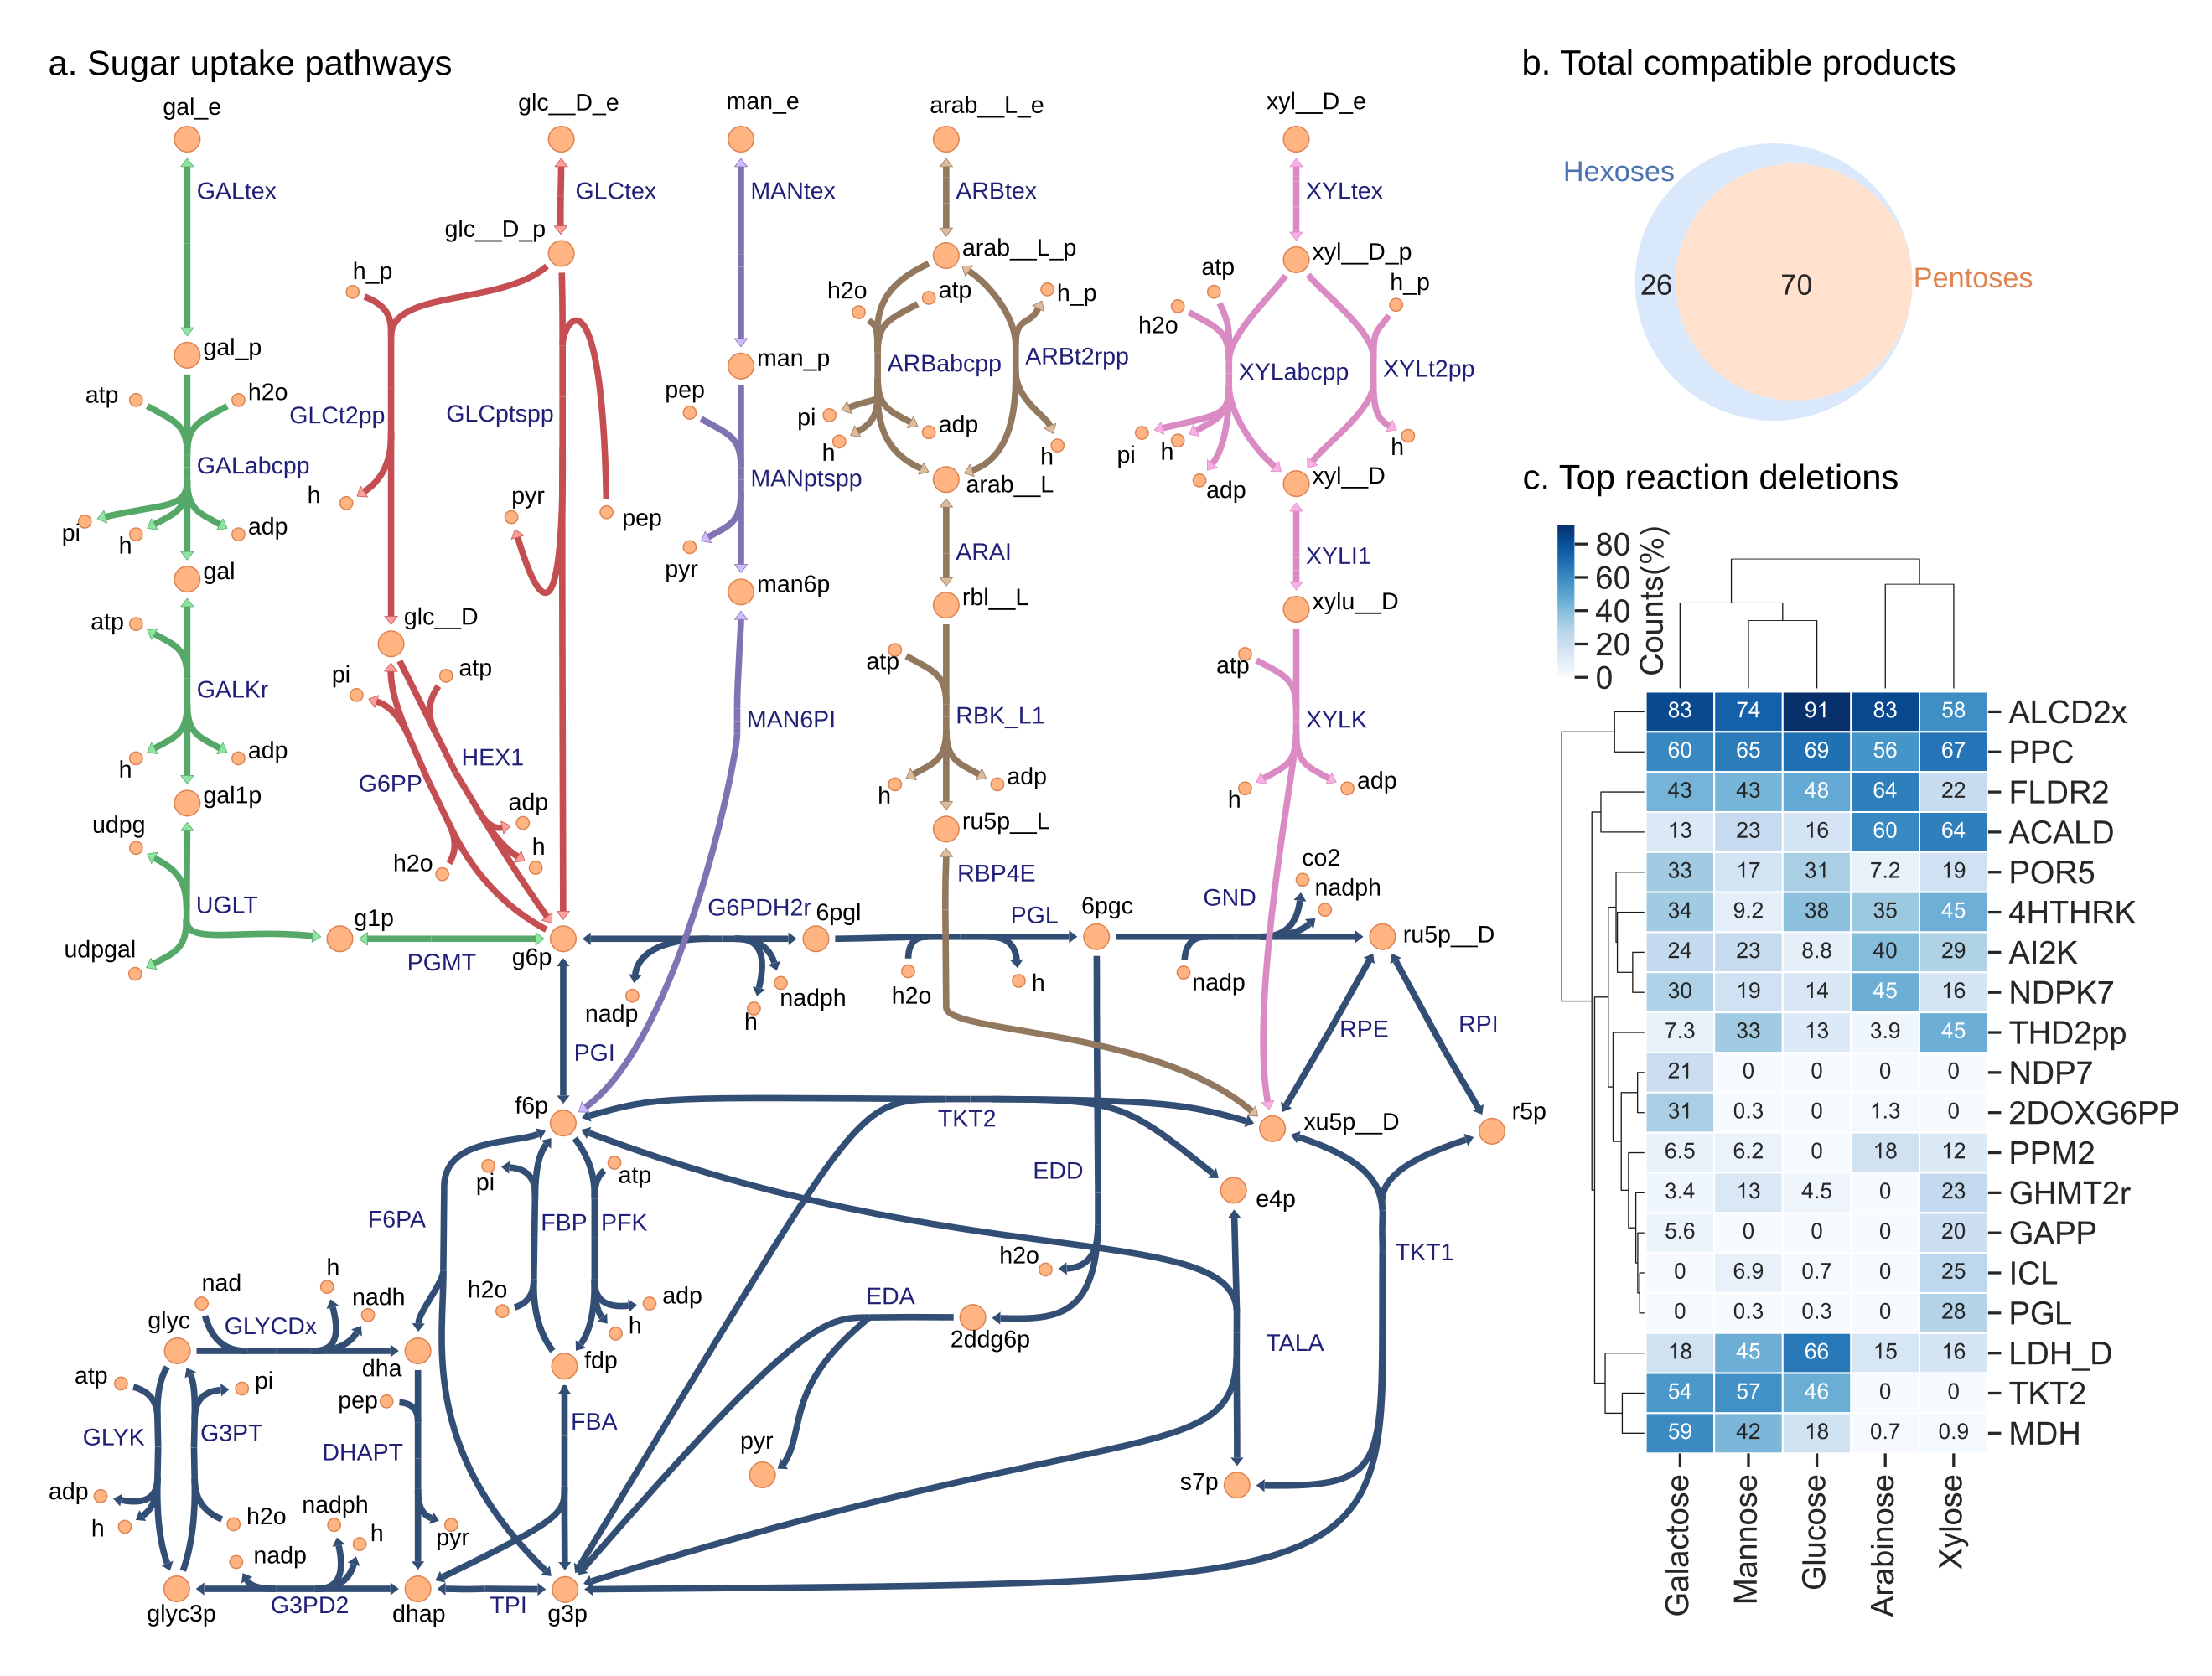
\includegraphics[width=1\textwidth,keepaspectratio]{sugars.png}
    \caption[Design of modular cells for different carbon sources ]{Design of modular cells for different carbon sources with design parameters $\alpha=10, \, \beta=2$. (a) Sugar uptake, pentose phosphate, Entner-Doudoroff, and upper glycolysis pathways. (b) Venn diagram of total products compatible with designs under pentoses and hexoses.
    The 26 products uniquely compatible with hexoses are:
    1agpg180, 2tdecg3p, 2agpg181, 3c3hmp, 3mob, 2hdecg3p, pe141, ps120, 1agpg160, 2agpg160, 23dhmb, ps141, 1agpe180, 2agpg180, apg120, 2agpe180, pe120, 2odec11eg3p, 4mop, lipidX, 3c2hmp, 2ippm, 2hdec9eg3p, 1agpg181, dha, 2odecg3p.
    (c) Top 20 reaction deletions according to deletion frequencies average across carbon sources. The counts for each carbon source correspond to the percentage of designs containing that reaction deletion.}
    \label{fig7:sugars}
\end{figure}


\paragraph{Unique metabolic features of pentoses limit their compatibility towards production modules that are compatible under hexoses}
%\paragraph{Certain production modules compatible under hexoses are incompatible with pentoses due to less metabolic possibilities of pentoses}
%- Limited ability to generate nadph due to incorporation downstream in the pentose phosphate pathway. This may indicate the use of MDH as a potentials ource of nadh
%- Limited ability to manipulate ppp reactions, most notably  TKT2
For the set of designs in each carbon source, we examined the total compatible products (i.e., number of unique products compatible in at least one design from the Pareto front).
This revealed a group of 26 products (27\% of the total 96 compatible products and 16\% of the original library size) that are only compatible in designs with hexose carbon sources  (Figure~\ref{fig7:sugars} b).
%Pentoses have a lower reduction potential and different uptake pathways than hexoses. %hence two features are
The incompatibility of these 26 products is likely due to the
 lower reduction potential and different uptake pathways of pentoses with respect to hexoses (Figure~\ref{fig7:sugars} a).
More specifically, we examined the most deleted reactions in each carbon source which revealed several differences in deletions between pentoses and hexoses (Figure~\ref{fig7:sugars} c).
Notably, pentoses do not use TKT2 and MDH reaction deletions, while hexoses make highly frequent use of them.
TKT2 is a key component of incorporating pentoses into glycolysis, and hence cannot be deleted by pentose consuming designs.
MDH  has been observed to be upregulated under anaerobic conditions when the sole carbon source is pyruvate, galactose, or xylose with respect to glucose.\citep{park1995}
Hence, MDH could be an important source of \textit{nadh} for substrates with less reduction potential.
Alternatively, MDH could also be important for \textit{nadph} generation as part of a pathway involving NADP-dependent Malic enzyme (ME2) that converts malate to pyruvate generating one mol of \textit{nadph}. % NOTE: THD2pp is present and can convert nadh to nadph more directly at no cost, so the use of MDH by pentose designs is not clear.
Overall, pentose uptake does not use the oxidative phase of the pentose phosphate pathway, the most important source of \textit{nadph} in \textit{E. coli},\citep{christodoulou2018}
hence limiting the products that can be growth-coupled to these carbon sources.
Further study of the reactions that limit pentose compatibility could enable strategies to overcome it in certain cases (e.g., create alternative sources of \textit{nadph} \citep{lee2013, ng2015c}).

% Of these 26 incopatible products which use nadhp?
% - 3-methyl-2-oxobutanotae  (3mob)
% - Fatty acids, as mentioned earlier

% Although if cofactor specificity, rather than redox  potential, is the limiting factor, that could be addressed by further engineering:
% https://link.springer.com/article/10.1007/s00253-013-4750-z


%TODO: Change section name
\subsection{Compatibility towards modules unknown at the time of chassis design}

\paragraph{There is a high correlation between design compatibility and its unknown product compatibility}
%\paragraph{Compatibility of a design towards the modules known at the time of design is is highly correlated with compatibility towards unknown modules}
% - Describe why is intersting
% - Describe approach: How to generate results and how to measure interesting feature (unknown compatibility)
% - Highlight correlation between known and unknown compatibility.
Given the vast space of potential modules, it is interesting to identify existing strains that can be repurposed for production of molecules not considered as part of the original strain design process.
To examine this scenario,  we randomly partitioned the product library into two evenly sized groups, and independently used each partition as input for ModCell-HPC.
This was done in triplicates that correspond to different random product partitions.
Hence, in each replicate there is a group of known products at the time of design and a group of unknown products. For the designs produced by ModCell-HPC, we computed their objective value and then compatibility towards unknown products, which we refer to as \emph{unknown compatibility} of a design, a useful metric to understand the potential to repurpose a given design.
In contrast, \emph{known compatibility} is the compatibility towards known products at the time of design, simply referred to as compatibility in previous cases study.
The total number of designs for each product group and the unknown compatibility distributions noticeably change across replicates (Figure~\ref{fig7:partitions} a).
Highlighting the important effect of known products in the resulting designs, which could be further explored to identify ``representative products" that can capture the necessary metabolic phenotypes required for certain product families. %TODO: Not very clear?
%Indicating that the specific input products can have an important effect in the unknown compatibility of the resulting designs.
%Indicating that there might be ``representative products" that can capture the necessary metabolic phenotypes required for certain product families.
Remarkably, there is a high correlation between known and unknown compatibility
of a given design (Figure~\ref{fig7:partitions} b-d).
Hence, highly compatible designs are better suited to be repurposed towards unknown products.

\begin{figure}[h]
    \centering
    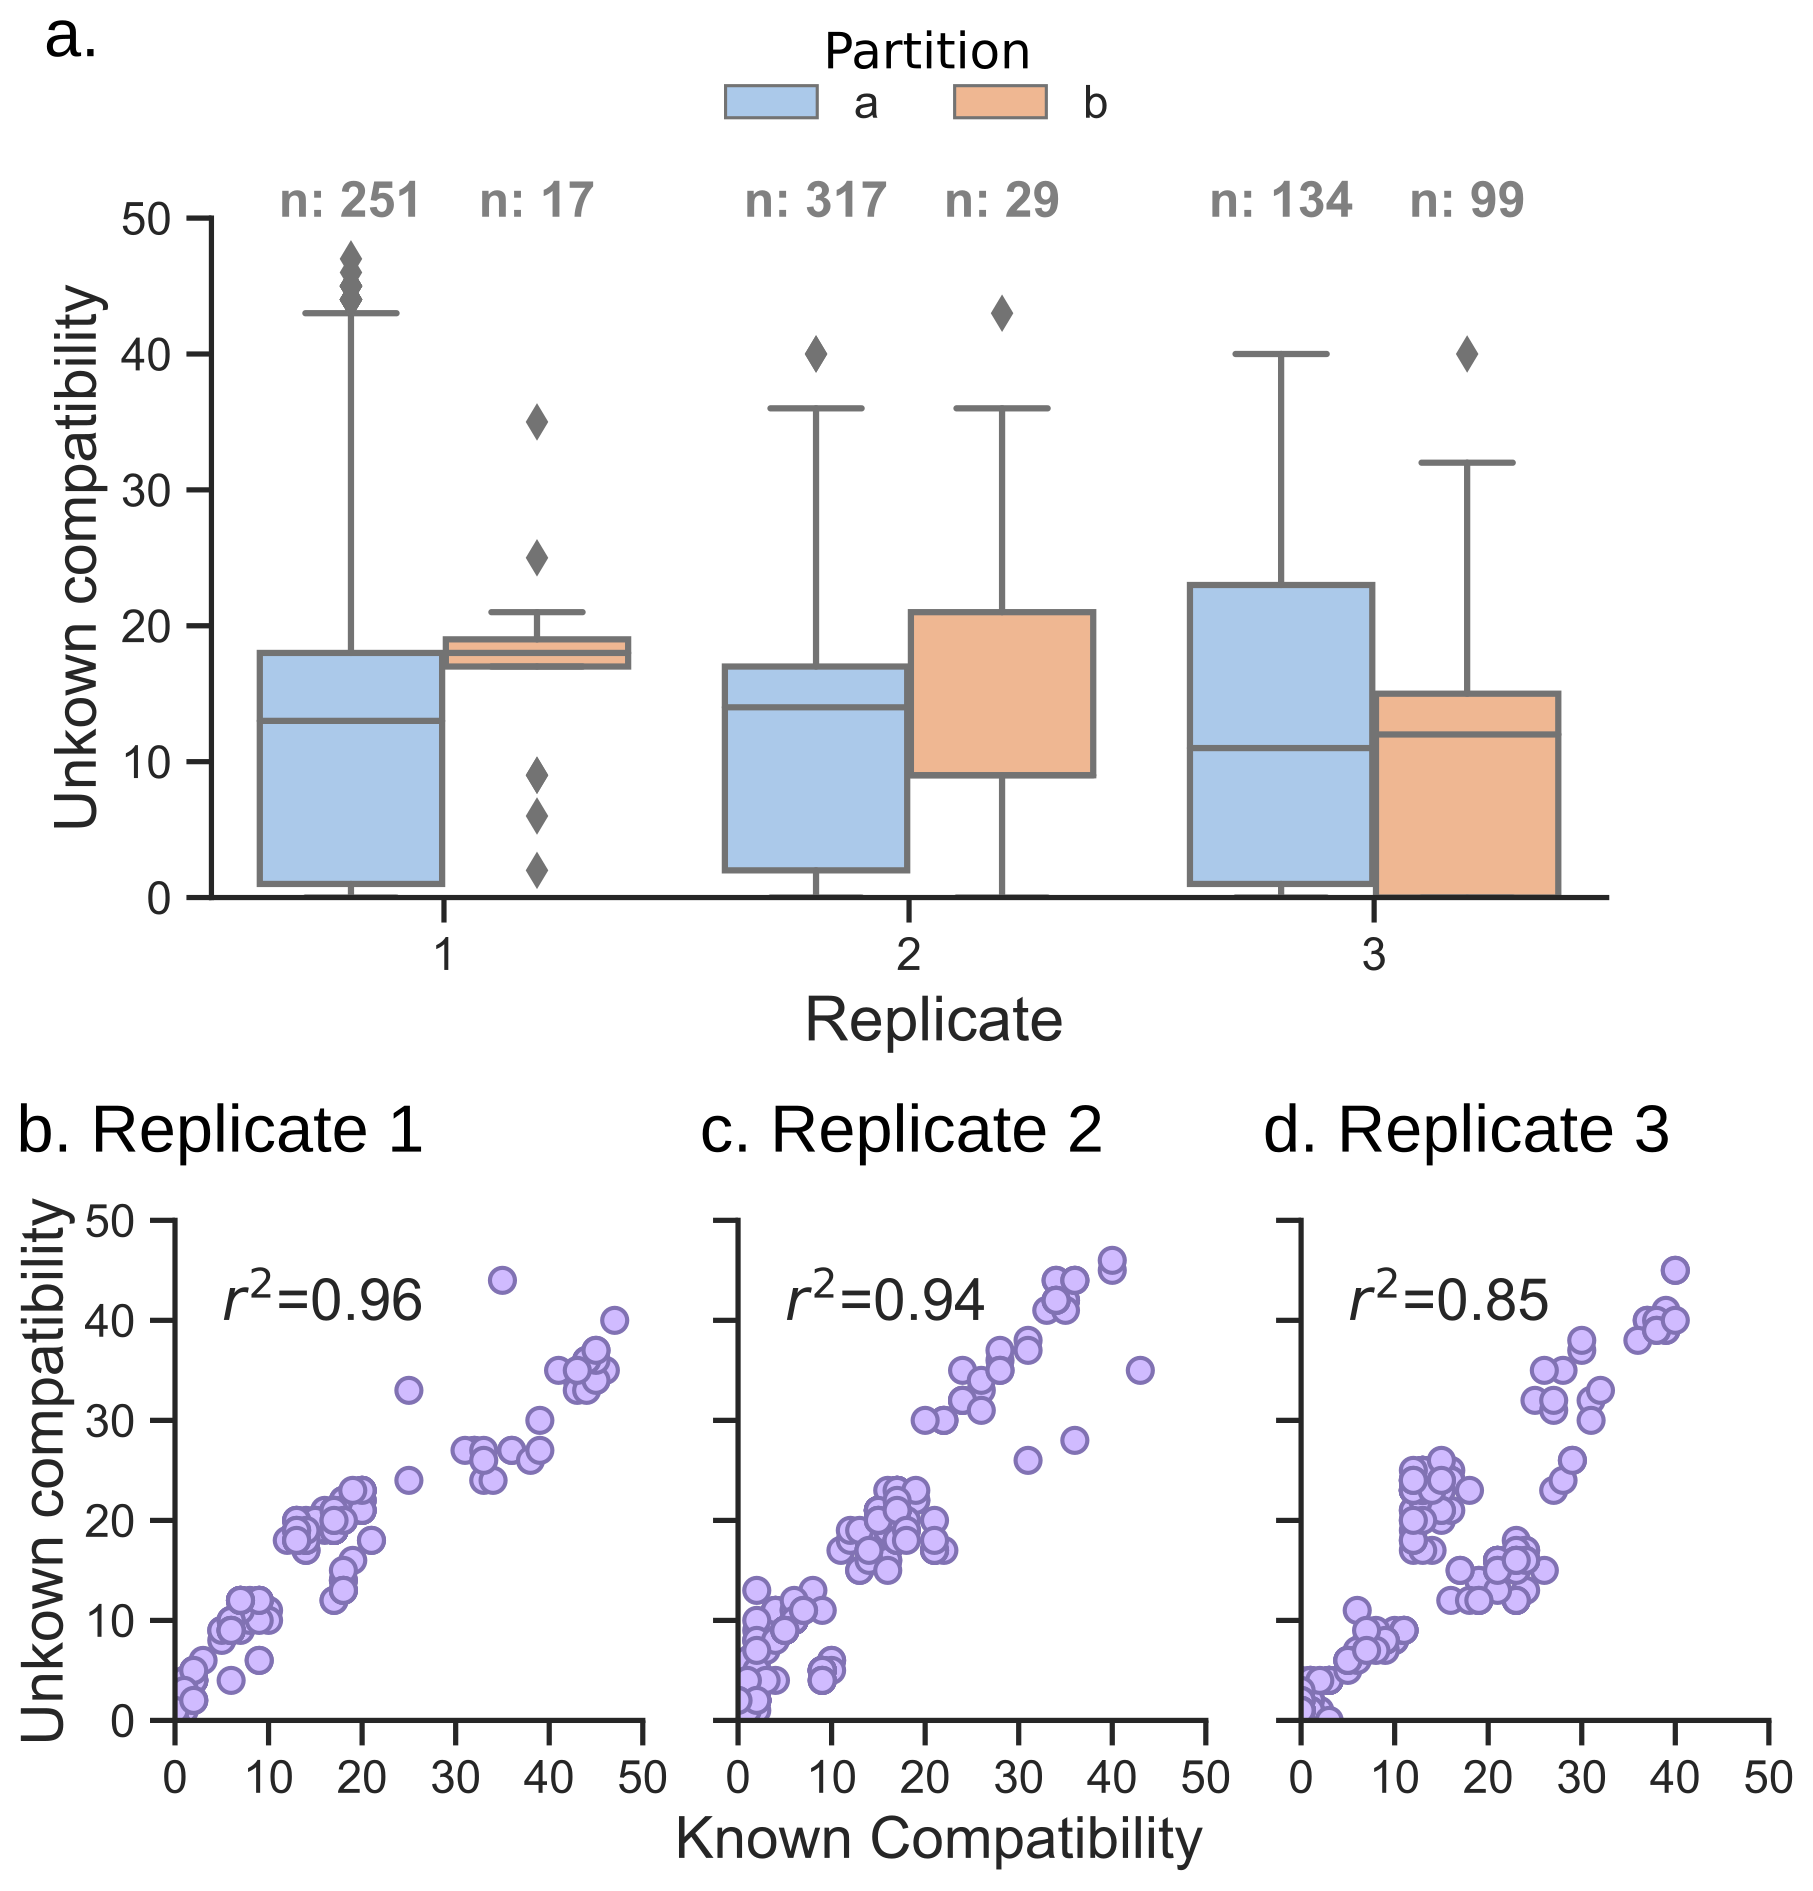
\includegraphics[width=.6\textwidth,keepaspectratio]{partitions.png}
    \caption[Compatibility towards unknown products]{Compatibility towards unknown products in 3 random even partitions of the product library. (a) Distribution of unknown compatibility, n corresponds to the number of designs in each case. (b-d) Comparison between unknown and known compatibility of each design for each replicate, $r^2$ is the Pearson correlation coefficient.}
    \label{fig7:partitions}
\end{figure}

\paragraph{Deletion reactions that remove major fermentation byproducts and alter redox metabolism have the highest contribution towards unknown compatibility}
%\paragraph{Reaction deletions that contribute the most towards unknown compatibility remove common fermentation byproducts followed by manipulations in redox metabolism}
% - Goal is to identify features of designs that contribute the most towards unknown compatibility
% - Describe approach
% - Conclude with LASER citation, this happen to be the intuitive strategies.

To identify the specific genetic intervention strategies that contribute to
the unknown compatibility of a design,  we defined the unknown compatibility contribution of deletion reaction $j$ ($ucc_j$) as follows:
\begin{equation}
    ucc_j=\frac{\sum\limits_{h\in\mathcal{H}_j} u_h}{|\mathcal{H}|}
\end{equation}
where $\mathcal{H}_j$ is the subset of designs from Pareto set ($\mathcal{H}$) containing deletion reaction $j$ and $u_h$ is the unknown compatibility of design $h$. %that corresponds to the compatibility towards modules not included as part of the ModCell-HPC input.
We computed $ucc$ for all 3 replicates and examined the top 10 sorted by mean value (Table~\ref{tab7:top10contrib}).
This revealed that the main contributors towards unknown compatibility are removal of major fermentative byproducts (lactate, ethanol, and acetate), indeed these are the strategies that repeat the most across the metabolic engineering literature,\citep{winkler2015} followed by manipulation of redox pathways (THD2pp, FLDR2, MDH) and metabolic branch points (TKT2, PPC).
Strain repurposing could be further explored with algorithms specialized for this task, e.g., by identifying module reactions in the unknown modules or using the existing strain as a starting point to identify genetic manipulations instead of a wild type strain.
In our analysis we have identified that high chassis compatibility and certain reaction deletions are indicators of compatibility towards unknown products.


\begin{table}[h]
    \caption[Top 10 reactions with highest unknown compatibility contribution]{Top 10 reactions sorted by mean unknown compatibility contribution ($ucc$) among replicates. }
    \centering
    \rowcolors{3}{gray!25}{white}
%\resizebox{1\textwidth}{!}{%
\begin{tabular}{llcccc}
\toprule
        &                                        &  \multicolumn{4}{c}{$ucc$}      \\
%\rowcolor{white}
%\rowcolors{2}{blue}{white}
%\cline{3-6}
\multirow{-2}{*}{ID} &    \multirow{-2}{*}{Name} &    R. 1 &    R. 2 &    R. 3                  &  Mean \\
\midrule
LDH\_D  &  D-lactate dehydrogenase & 13.2 & 10.5 & 11.9 & 11.9 \\
ALCD2x &  Alcohol dehydrogenase (ethanol) & 11.5 & 10.5 & 11.8 & 11.3 \\
PTAr   &  Phosphotransacetylase & 4.0 & 4.8 & 6.5 & 5.1 \\
ACALD  &  Acetaldehyde dehydrogenase (acetylating) & 4.5 & 2.8 & 2.9 & 3.4 \\
THD2pp &  NAD(P) transhydrogenase (periplasm) & 4.7 & 2.4 & 2.2 & 3.1 \\
ACKr   &  Acetate kinase & 3.8 & 2.2 & 1.7 & 2.6 \\
FLDR2  &  Flavodoxin reductase (NADPH) & 2.0 & 2.2 & 2.9 & 2.4 \\
TKT2   &  Transketolase & 2.6 & 2.0 & 2.5 & 2.4 \\
PPC    &  Phosphoenolpyruvate carboxylase & 2.3 & 2.2 & 2.5 & 2.3 \\
MDH    &  Malate dehydrogenase & 2.7 & 1.1 & 2.3 & 2.0 \\
\hline
\end{tabular}%}

    \label{tab7:top10contrib}
\end{table}

\section{Conclusions}
% - Develop modcell-hpc:
%       - What does it do
%       - Why is it useful
% - What do we find by applying modcell-hpc?
%
% - What are future challenges/directions?
%
% What are key aspects of the method developed here?
% What are key insights in the design of platform strains that result from applying the method?

% Some random points
%Notably, only a few genetic manipulations seem to be sufficient ...
%
%While current genetic engineering techniques may limit the validation of such system, due to the slow of product pathway construction and overexpression...
%
%- While growth coupling has advantages ...., such tight coupling, if implemented successfully, can not only be relevant at the pathway optimizataion stage, but also at the scaling up stage where loss of phenotype may occur. However, such design might be too strict and not be practical for all metabolites of interest. %(Make this claim on the basis of what results? Maybe only around 50\% of the library
%
%
%Remarkably, the proposed designs are consistent with isolated metabolic engineering strategies, reinforcing the potential for generalization of certain approaches.
%select good candidate products thorugh
%Further analysis at the metabolic strategies behind these designs revealed...
%
%%We identified a variety of designs, each compatible with dozens of products.

In this study we developed ModCell-HPC, a computational method to design modular platform strains compatible with hundredths of product synthesis modules.
We applied ModCell-HPC to a library of 161 products derived form the endogenous metabolism of \textit{E. coli} and used this same organism as a chassis.
This resulted in many Pareto optimal designs for the production of these molecules, from which we selected the smallest set of designs necessary to ensure any compatible product is present in at least one of them.
The designs feature strategies consistent with previous experimental studies aimed at optimizing production of a single product, reinforcing our confidence in the value of our simulations.
Remarkably, the strategies feature not only removal of major byproducts (e.g., lactate, ethanol), but also modification of key metabolic branch-points (e.g., deletion of TKT2 that alters flux between pentose phosphate and glycolysis pathways; or PPC, that alters flux from glycolysis towards the Krebs cycle).
We used growth-coupled to product formation as a target phenotype for each production module,
such platform strains can also enable high-throughput pathway engineering approaches, e.g., the chassis can be simultaneously combined with a library of modules to rapidly identify good candidate pathways through adaptive laboratory evolution.
We also used ModCell-HPC to design high compatibility platform strains to utilize different carbon sources, revealing the limitations of pentoses that might be addressed by redox cofactor engineering.
Finally, we used ModCell-HPC to investigate how existing strains might be repurposed towards products unknown at the time of design, and identified (known) compatibility and specific reaction deletions as important features of highly repurposable strains.
Overall, ModCell-HPC is an effective tool towards more efficient and generalizable design of modular platform strains that have recently captured the interest of metabolic engineers. \citep{nielsen2016}


%\singlespace



\section*{Supplementary Materials}
\begin{enumerate}%[label=Supplementary Material \arabic*, leftmargin=*]
    \item Supplementary text, figures, and tables. \label{sm:figures}
    \item Designs for selected parameters $\alpha=5,\,\beta=1$. \label{sm:designs}
    \item Computer programs used to generate the results of this study. \label{sm:code}
    %\item NOTE: what to do with reaction/metabolite abbreviations?
\end{enumerate}


    
\renewcommand{\thefigure}{\roman{figure}} % See here for other options: http://timmurphy.org/2011/07/18/latex-table-and-figure-numbering-style/
\setcounter{figure}{0}

\chapter*{Future directions}\label{ch:conclusion}
\addcontentsline{toc}{chapter}{Future directions}

% Main points:
% - What has been accomplished that was not there before
% - What is the most relevant follow up work
% - What are the most relevant challenges
% - Make sure to connect with the introduction, that is refer to the problems presented there and the degree to wich they are addressed.


% 1. Accomplishments (Separate technical and scientific?)
% - Use of system level models
% - Develop multi-objective optimzation formualtions and solution techniques, with the primary aim of modular design, but applicable to many design and analysis situtations were multiple conflicting objectives exist -> for example?
% - ...
% - (reference to the arrow figure)


%TODO: Could move the contribution to later in the pargraph?
%In this thesis we have developed quantitative and systematic tools for modular design of cellular systems, primarly through multi-objective optimization theory.
%The driving application behind these developments is
Whole-cell biocatalysis technology can lead to renewable and sustainable manufacturing of chemicals, fuels, and materials.
Over the past two decades, researchers at companies and universities have been developing platform strains that can produce various metabolically similar molecules \citep{nielsen2016}.
However, these efforts have been limited by the use of qualitative and reductionistic approaches.
Motivated by the potential of modular platform strains, we used multi-objective optimization theory and  genome-scale metabolic models to develop several iterations of the ModCell design method (Figure~\ref{fig8:arrow}).
We applied ModCell tools to design \textit{E.~coli} and \textit{C.~thermocellum} modular cells that enable various product synthesis phenotypes in a plug-and-play fashion.
These proposed modular cell designs require few genetic manipulations thanks to the natural modular features of metabolic networks.
Overall, this effort contributes to the current wave in synthetic biology of tackling problems through more quantitative and holistic approaches.
We envision the new design tools will help reduce the cost and time required to develop efficient and robust biocatalytic strains that harness the large space of molecules resulting from natural and synthetic metabolic pathways.

\begin{figure}[h]
  \centering
  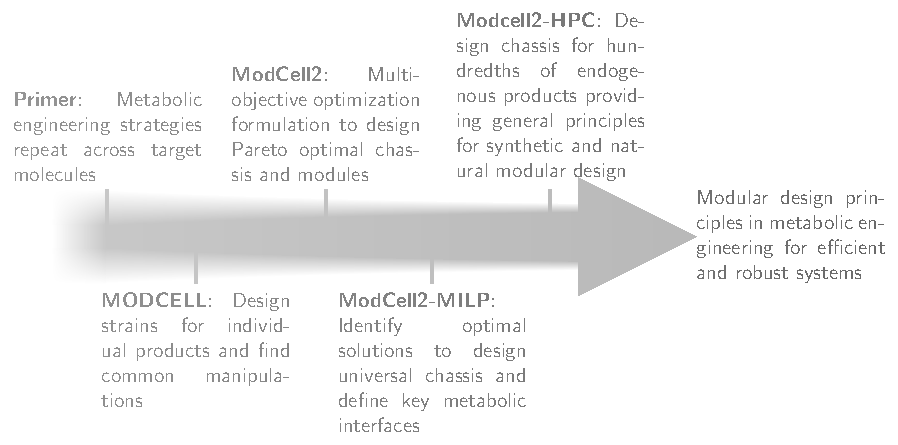
\includegraphics[width=.95\textwidth]{timeline-arrow}
    \caption[Developments in modular cell design tools]{Developments in modular cell design tools: Primer (Chapter~\ref{ch:review}), MODCELL \citep{trinh2015}, ModCell2 (Chapter~\ref{ch:modcell2}), ModCell-MILP (Chapter~\ref{ch:milp}), ModCell-HPC (Chapter~\ref{ch:hpc}).}
    \label{fig8:arrow}
\end{figure}


% 2. Next wave: The need of the problem framing to build and study strains in this context
% - While techniques have general application,  Predictions without validation is only part of the story.
% - There are two views: 1)design simulation to build; 2)Use simulation to contextualize
% - Modcell falls in case 1. The problem formulation requires that experimental data is ... this was as much as possible done by examining the literature, primarly in the field of metabolic engineering, where genetic manipulations are implemented and characterized ...
% - C therm chapter is case 2.
% - Next wave -> build and characterize

% TODO: The main point does not stand out, and the beginning of the paragraph feels confusing
The interdisciplinary nature of computational biology demands that one addresses algorithmic and modeling challenges, while also combining simulation efforts with experimental validation.
To bridge the gap between simulations and experiments, a simulation can be used to generate a testable hypothesis, or a simulation can be used to explained existing data.
Chapter~\ref{ch:ctherm} is an example of the second case, where proteomics data studied through model simulations increases our understanding of redox metabolism in \textit{C.~thermocellum} biofuel-producing strains.
However, the majority of this work, formulated as a biocatalysis strain design problem, falls under the first case.
Hence, the next wave of development of modular cell design principles should be focused on the implementation and characterization of the strains proposed here, closing the design-build-test-learn cycle.

%post hoc addition of experimental data %Watch out since post hoc, can have quite negative connotations %Watch out since post hoc, can have quite negative connotations


% 3. Future perspective (be general and tie back to the **intro**)
% - Main challenges in the relevant fields
% - highly predictive does not seem around the corner
% - time horizon for application
% - Ethical concerns: Increased inequality and existential risk

As with most contemporary research works, this thesis contributes a drop to the ocean of knowledge needed to address the scientific and social challenges of our time.
%Scientific and social challenges,
The implementation of modular design principles developed here can be impactful in addressing the challenge of whole-cell biocatalysis, however, there are other important facets of this problem.
%There are multiple relevant facets to the problem of whole-cell biocatalysis.
Most notably, the predictive and explanatory capacities of cellular models remain highly limited by a lack of tools to integrate disparate data types and to efficiently measure enzymatic kinetics.
%integration ability to integrate disparate data types and the technical challenges of measuring certain parameters such as the catalytic efficiency of each enzyme.
Furthermore, even if the necessary metabolic fluxes and required enzyme concentrations were known, it remains highly challenging to accomplish appropriate enzyme expression and pathway function \textit{in vivo}.
More generally, we lack precise comprehensive description of already known phenomena (e.g., metabolic reactions), and unknown or poorly explored biophysical phenomena (e.g., macromolecular crowding) are likely to highly influence cellular function.
Hence, it is unlikely that we will develop the capacity to manipulate living organisms for any conceivable biological function in a near future.
The good news is that we are rapidly overcoming the key challenges needed for applied technologies, as evidenced by the many biotechnology companies emerging over the last decade.

As we develop novel technologies, we must also become aware of the ethical and existential risks associated with them.
For example, genetic engineering for enhanced cognitive abilities could likely become an expensive medical treatment that increases the wealth gap in society.
These concerns are specially relevant for the field of synthetic biology, as tools continue to become more widely available hence enabling DIY biohacking \citep{bennett2009}.
These developments could pose an existential risk for our current civilization, given that a highly destructive technology becomes sufficiently easy to use,  and such technology cannot be ``uninvented" or effectively policed.
This challenge can be illustrated through The Urn of Inventions metaphor (Figure~\ref{fig8:vwh}) \citep{bostrom2019}. % NOTE: Follow up this sentence to expl
% NOTE: Make sure this feels "complete" but that further reading is available to expand, do not lean on citations. It has to make sense entirely in this context.
% NOTE: Last sentence needs to be conclusive
Briefly, consider technologies to be balls in an urn, and our current strategy is to draw balls as fast as possible, perhaps to obtain wealth, prestige, and citations.
If there is a ``black ball'' technology, which discovery would cause high damage, alternative research strategies should be considered.
In summary, while issues like climate change already receive considerable attention, we should become more aware of other dangers of technological development and create policies accordingly.

\begin{figure}[h!]
  \centering
  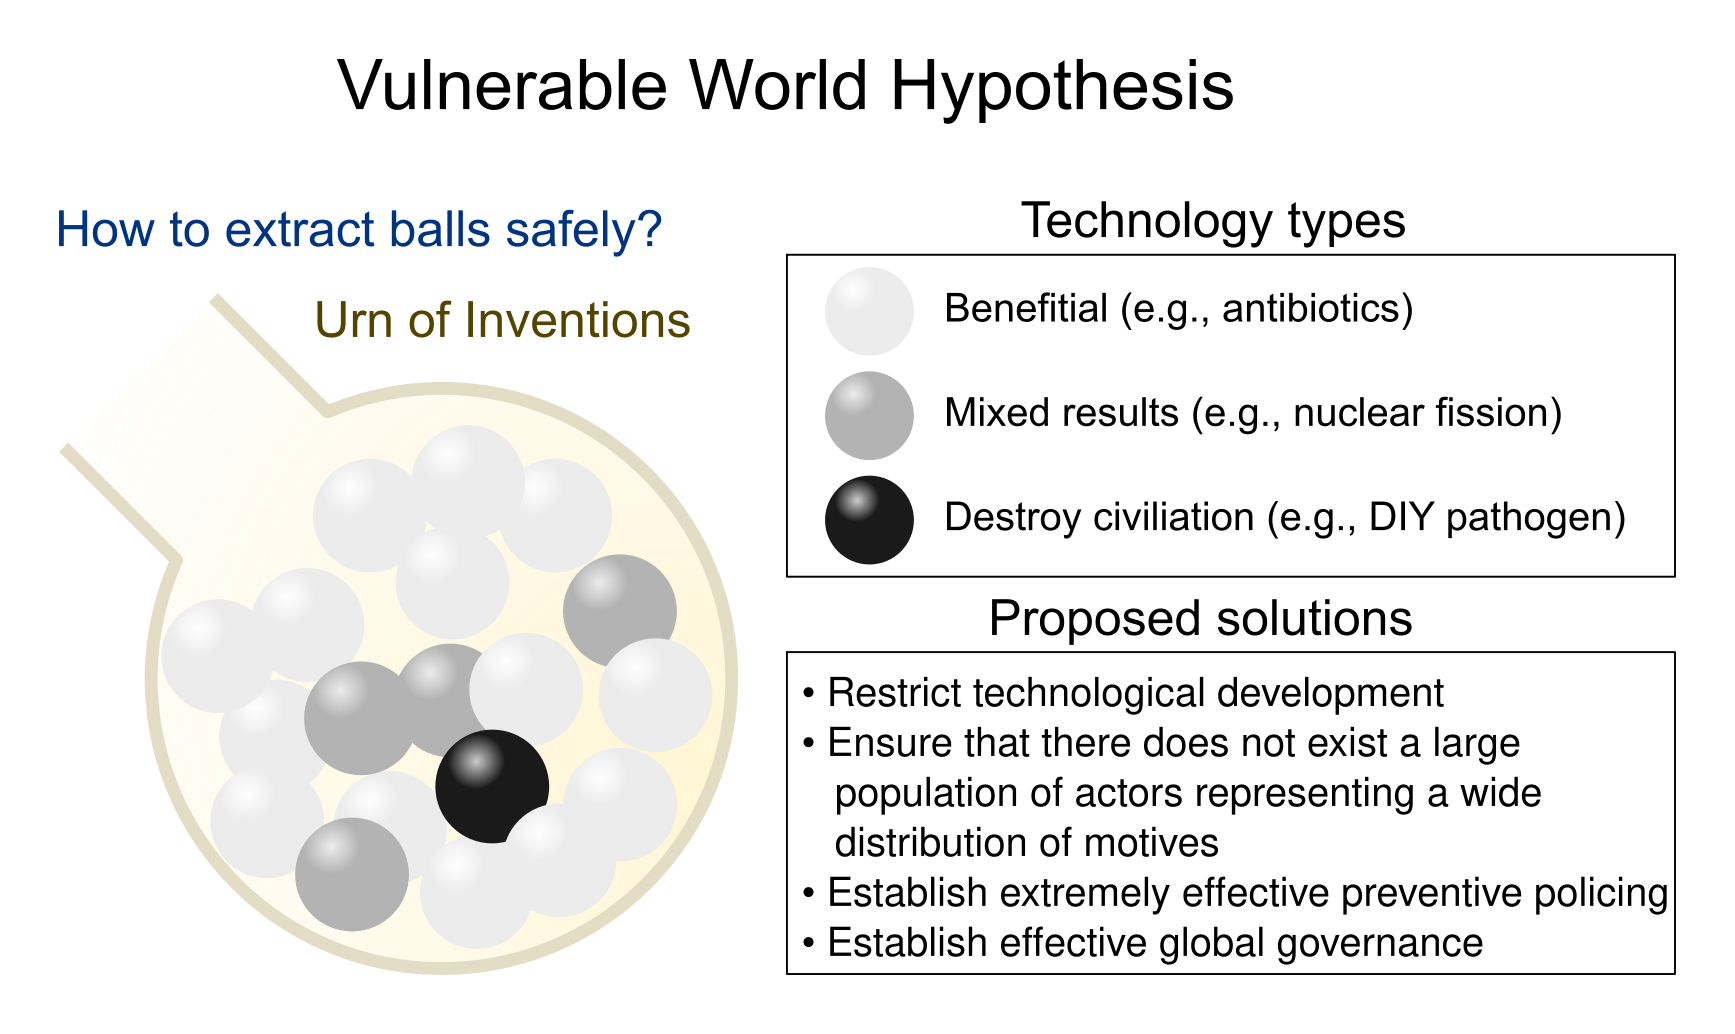
\includegraphics[width=.83\textwidth]{urn-of-inventions}
    \caption[The Vulnerable World Hypothesis]
    {The Vulnerable World Hypothesis illustrated through the Urn of Inventions metaphor \citep{bostrom2019}.}
    %{According to the The Vulnerable World Hypothesis, there exists a technology that if discovered would have devastating effects to civilization. %If the hypothesis is true, we should reconsider how scientific and technological discovery is to be conducted to minimize such risk.
    %See \citep{bostrom2019} for further details.}
    \label{fig8:vwh}
\end{figure}

    %%%%%%%%%%%%%%%%%%%%%%%%%%%%%%%%%%%%%%%%%%%%%%%%%%%%%%%%%%%%%%%%%%%%%%%%%%%%%%%%%%%%%%%%%%%%%%%%%%%%%
    % BIBLIOGRAPHY
    %%%%%%%%%%%%%%%%%%%%%%%%%%%%%%%%%%%%%%%%%%%%%%%%%%%%%%%%%%%%%%%%%%%%%%%%%%%%%%%%%%%%%%%%%%%%%%%%%%%%%
    \makeBibliographyPage % make the bibliography title page
\newpage

% To make the bibliography, use \utbiblio{#1}{}{} command. Always use "#1" for the first entry. The second entry is your bibliography style, and the third entry is the name of your bibliography file (.bib file extension)
% bibliography style - recommend using apalike-doi as it hyperlinks DOIs
% Be sure to run BibTeX in order to generate the bibliography correctly.

\utbiblio{#1}{apalike}{bibliography}

    %%%%%%%%%%%%%%%%%%%%%%%%%%%%%%%%%%%%%%%%%%%%%%%%%%%%%%%%%%%%%%%%%%%%%%%%%%%%%%%%%%%%%%%%%%%%%%%%%%%%%
    % APPENDIX - OPTIONAL - COMMENT OUT IF NOT NEEDED
    %%%%%%%%%%%%%%%%%%%%%%%%%%%%%%%%%%%%%%%%%%%%%%%%%%%%%%%%%%%%%%%%%%%%%%%%%%%%%%%%%%%%%%%%%%%%%%%%%%%%%
    % Appendix can be used for supplementary material

    \makeAppendixPage{2}   % Input the number of appendices
    \appendix
    \section{Supplementary Material 1 for Chapter 3}

%\counterwithin{figure}{section}

\newcommand{\hbAppendixPrefix}{A}
%
\renewcommand{\thefigure}{\hbAppendixPrefix\arabic{figure}}
\setcounter{figure}{0}
\renewcommand{\thetable}{\hbAppendixPrefix\arabic{table}}
\setcounter{table}{0}
\renewcommand{\theequation}{\hbAppendixPrefix\arabic{equation}}
\setcounter{equation}{0}

\begin{figure}[h]
  \centering
  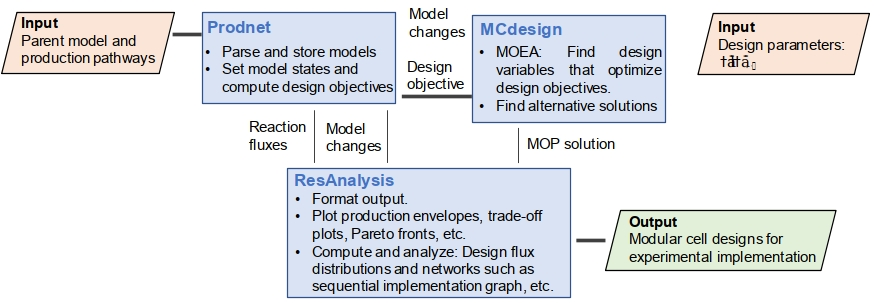
\includegraphics[width=\textwidth]{ms1-sf1}
    \caption[Software architecture of ModCell2]{Software architecture of ModCell2. The Prodnet class preprocesses production network models and computes design objectives. The MCdesign class serves as an interface between the MOEA optimization method and metabolic models. The ResAnalysis class loads the Pareto set computed by MCdesign and performs analyses to identify the most promising designs.}
\end{figure}

\begin{figure}[h]
  \centering
  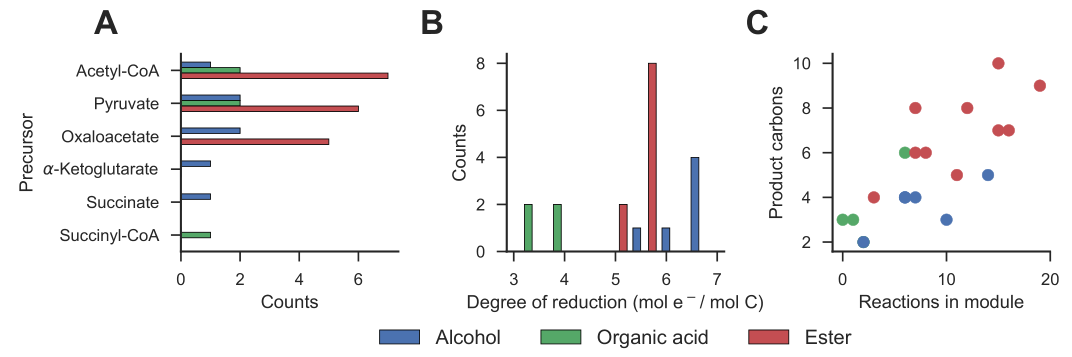
\includegraphics[width=\textwidth]{ms1-sf2}
    \caption[Biochemical properties of production modules]{Properties of 20 production modules used in the E. coli genome-scale metabolic model for biosynthesis of 6 alcohols, 4 organic acids, and 10 esters. (A) Distribution of precursor metabolites. (B) Distribution of degrees of reduction of target products. (C) Correlation between the number of product carbons and the number of reactions in production modules. Alcohols include ethanol, propanol, butanol, isobutanol, pentanol, and 1,4-butandiol; acids include pyruvate, D-lactate, acetate, and adipic acid; and esters include ethyl acetate, propyl acetate, isobutyl acetate, ethyl butanoate, propyl butanoate, butyl butanoate, isobutyl butanoate, ethyl pentanoate, isobutyl pentanoate, and pentyl pentanoate.
    }
\end{figure}

\begin{figure}[h]
  \centering
  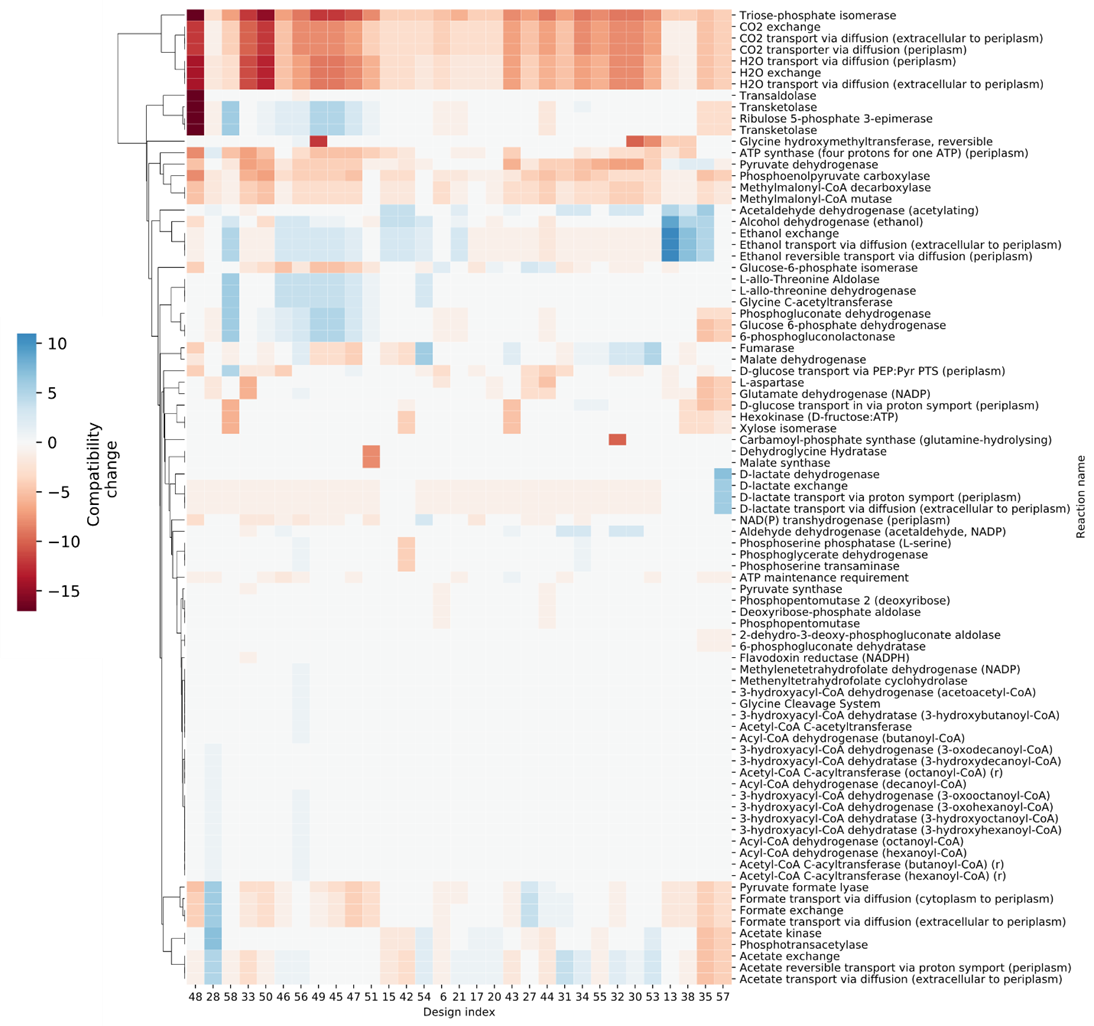
\includegraphics[width=\textwidth]{ms1-sf3}
    \caption[Robustness analysis of designs]{Robustness analysis for wGCP-4-0 designs for the E. coli genome scale model. Only the designs that are compatible with 4 or more products (compatibility  4) were considered. Each column corresponds to a design whereas each row corresponds to a single-reaction deletion. Included in the heat map are all reaction deletions with a compatibility change that is not 0 in at least one product.
    }
\end{figure}

\begin{figure}[h]
  \centering
  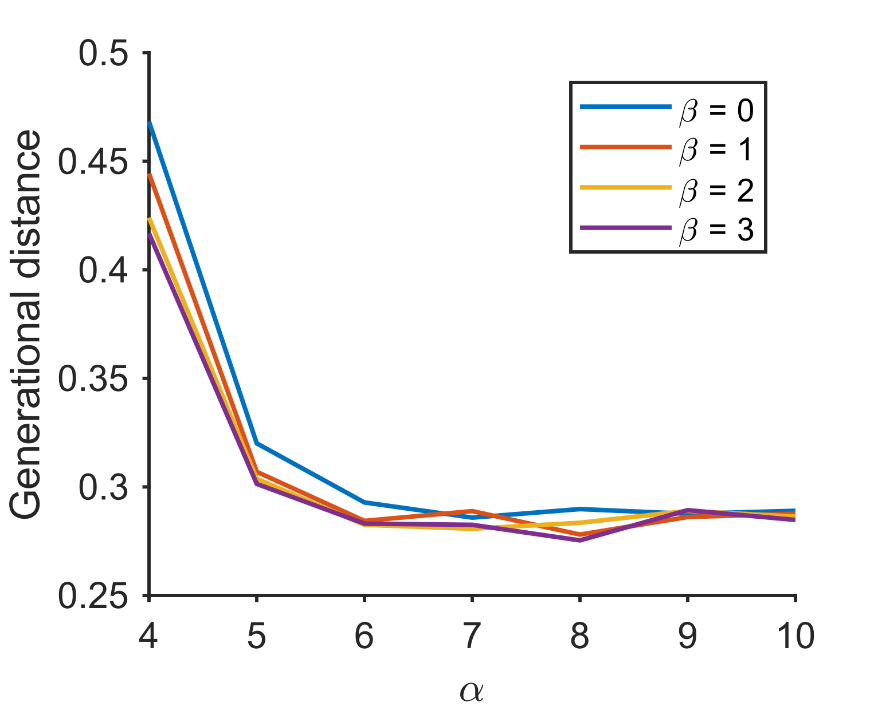
\includegraphics[width=.5\textwidth]{ms1-sf4}
    \caption[Generational distance among different design parameters]{Generational distances between the calculated Pareto fronts and the reference utopia point. The generational distance is calculated as follows: $GD=\frac{\left|d\right|_2}{\left|d\right|_1}$where  $d_j=\left| \PF^j - \PFs \right|_2$ where $\PF$ is the calculated pareto front and $\PFs=\vec{1}$ is the utopia point. A smaller value of $\mathit{GD}$ indicates the overall objective values in the Pareto front are closer to the utopia point. The calculation was performed for the iML1515 model with 20 products using the wGCP objective, various  and  values, and a run time of 10 h for all cases.
    }
\end{figure}

    \newcommand{\paragraphit}[1] {\paragraph{\textit{#1}}}

\renewcommand{\hbAppendixPrefix}{B}

\renewcommand{\thefigure}{\hbAppendixPrefix\arabic{figure}}
\setcounter{figure}{0}
\renewcommand{\thetable}{\hbAppendixPrefix\arabic{table}}
\setcounter{table}{0}
\renewcommand{\theequation}{\hbAppendixPrefix\arabic{equation}}
\setcounter{equation}{0}

\section{Supplementary Material 2 for Chapter 3}


%\documentclass{article}
%\usepackage{supmaterial}
%
%\title{Supplementary File S1 \\
%	\large Multiobjective Strain Design: A Framework for Modular Cell Engineering}
%
%\author[1,2]{Sergio Garcia}
%\author[1,2,*]{Cong T. Trinh}
%\affil[1]{Department of Chemical and Biomolecular Engineering, The University of Tennessee, Knoxville, TN}
%\affil[2]{Center for Bioenergy Innovation, Oak Ridge National Laboratory, Oak Ridge, TN}
%\affil[*]{Corresponding author: Tel: 865-974-2181. Email: ctrinh@utk.edu.}
%
%\begin{document}
%{\let\newpage\relax\maketitle}
%\tableofcontents
%\newpage

\subsection{Solution method: Multiobjective Evolutionary Algorithm}

\subsubsection{Definitions}
\paragraph{Terms}
\begin{description}
\item[Parent network:] A parent network is a metabolic model of a host organism that is used to construct a modular cell.
\item[Production module:] A production module is a metabolic pathway that is added to a modular cell to synthesize a target product.
\item[Production network:] A production network is a combination of a parent network and a production module.
\item[MOEA:] Multiobjective evolutionary algorithm.
\end{description}

\paragraph{Sets}
\begin{description}
\item[$\mathcal{I}_k:$] Set of metabolite indices in production network $k$.
\item[$\mathcal{J}_k:$] Set of reaction indices in production network $k$.
\item[$\mathcal{K}:$] Set of production network indices.
\item[$\mathcal{C}$]: Set of candidate reaction deletion indices, where $\mathcal{C} \subseteq \mathcal{J}^{parent} \subseteq \mathcal{J}_k \;, \forall k \in \mathcal{K}$.
\end{description}

\paragraph{Continuous variables}
\begin{description}
\item[$v_{jk}:$] Flux of reaction $j$ in production network $k$.
\item[$v_{Pk}:$] Flux of target product (P) reaction in production network $k$.
\item[$v_{Xk}:$] Flux of biomass (X) synthesis reaction in production network $k$.
\item[$f_k:$] Objective function for production network $k$.
\item[$f_k^{wGCP}:$] \textit{wGCP} objective function for production network $k$.
\item[$f_k^{sGCP}:$] \textit{sGCP} objective function for production network $k$.
\item[$f_k^{NGP}:$] \textit{NGP} objective function for production network $k$.
\item[$p_k:$] Penalty objective function for production network k.
\item[$q^{enum}:$] Objective function for enumerating alternative solutions.
\end{description}

\paragraph{Binary variables}
\begin{description}
\item[$y_j:$] Reaction deletion indicator that takes a value of 0 if reaction $j$ is deleted in a modular cell, and 1 otherwise.
\item[$z_{jk}:$] Endogeonous, module-specific reaction indicator that takes a value of 1 if reaction $j$ is added back to the production module in network $k$, and 0 otherwise.
\item[$d_{jk}= y_j \lor z_{jk}:$] Modeling variable which takes a value of 1 if reaction $j$ may carry flux in production network $k$, and 0 otherwise.
\end{description}

\paragraph{Parameters}
\begin{description}
\item[$S_{ijk}:$] Stoichiometric coefficient of metabolite $i$ in reaction $j$ of production network $k$.
\item[$l_{jk}:$] Lower bound flux for reaction $j$ in production network $k$.
\item[$u_{jk}:$] Upper bound flux for reaction $j$ in production network $k$.
\item[$\alpha:$] Maximum number of deletion reactions in a modular cell.
\item[$\beta_k:$] Maximum number of endogenous module-specific reactions in the module of production network $k$.
\item[$\epsilon:$] Small scalar used for tilting the biomass objective function to obtain the minimum product rate available at the maximum growth rate. In the simulation, we used $\epsilon=0.0001$.
\end{description}

\subsubsection{Solver} \label{sec:mainMOP}
We used the \textit{gamultiobj()} solver, an implementation of NSGA-II \citep{deb2002}, from the MATLAB Optimization Toolbox to solve our combinatorial multiobjective optimization, formulated as an unconstrained multiobjective problem of
the form:
\begin{equation}
\max (p_1,p_2,\dots ,p_{|\mathcal{K}|})^T
\end{equation}
with a \textit{bitstring} population type where each individual is a binary vector corresponding to the design variables $y_j$ (reaction deletions) and $z_{jk}$ (endogenous module-specific reactions). To enforce the constraints on the number of deletion and endogenous module reactions, a penalty function $p_k$, instead of $f_k$, (Section \ref{sec:penalty}) and customized genetic operators (Section \ref{sec:customOp}) were used, respectively. %The design objective values are computed during the MOEA objective function evaluation by solving the associated linear programs ((\ref{eq:rpgLP}) for wGCP, and additionally  (\ref{eq:rpngLP}) for sGCP).

\subsubsection{Penalty Objective function} \label{sec:penalty}

To restrict the maximum number of reaction deletions, we optimized the following penalty function $p_k$ instead of $f_k$:

\begin{equation} \label{eq:pkp}
p_k =
\begin{dcases}
\frac{f_k}{\displaystyle \sum_{j\in C} (1-y_j)} & \text{if}\;  \sum_{j\in C} (1-y_j) > \alpha\\
f_k & \text{otherwise}
\end{dcases}
\end{equation}
The penalty function is designed to decrease $f_k$ of an individual proportionally to the number of deletion reactions exceeding the set limit $\alpha$. Implementation of this penalty function helps the  optimization problem converge rapidly because favorable deletion reaction candidates are likely kept to obtain desirable solutions. After simulation, only solutions satisfying the maximum reaction deletion constraint are preserved to obtain the Pareto set of our original problem.

\subsubsection{Design objective computation} \label{sec:design_obj_comp}
Depending on desirable applications, the following design objectives are considered:
\begin{alignat}{3}
	f_k^{wGCP} & =\frac{v_{Pk}^{\mu}}{v_{P_{max}k}^{\mu}}\in[0,1], \qquad & & \forall k\in \mathcal{K} \label{eq:obj_wgcp}\\
	f_k^{sGCP} & =\frac{v_{Pk}^{\mu}}{v_{P_{max}k}^{\mu}} \, \frac{v_{Pk}^{\bar{\mu}}}{v_{P_{max}k}^{\bar{\mu}}} \in[0,1], \;  & &  \forall k\in \mathcal{K} \label{eq:obj_sgcp}\\
	f_k^{NGP} & = \frac{v_{Pk}^{\bar{\mu}}}{v_{P_{max}k}^{\bar{\mu}}} \in[0,1], \qquad  & &  \forall k\in \mathcal{K} \label{eq:obj_ngp}
	\end{alignat}

%The design objectives  (\ref{eq:obj_wgcp})-(\ref{eq:obj_ngp}) feature product and biomass metabolic fluxes at key cellular states. These fluxes are determined using steady-state constraint based models of metabolism. Each target product is represented by a separate model. Depending on the design objective, additional constraints must be imposed to the model, such as the need for cell growth, or the absence of cell growth. First, we present the space of steady-state reaction fluxes of production network $k$, when a minimum amount of cell growth is required:

\noindent In \eqref{eq:obj_wgcp}-\eqref{eq:obj_ngp}, the terms $v_{Pk}^{\mu}$, $v_{P_{max}k}^{\mu}$, $v_{Pk}^{\bar{\mu}}$, and $v_{P_{max}k}^{\bar{\mu}}$ are computed by solving the following linear programming problems:

\begin{alignat}{3}
& v_{Pk}^{\mu} 	&\in& \,	\text{arg }	\underset{}{\text{max}} \{v_{Xk}-\epsilon v_{Pk} : v_k\in \Pi_k^{\mu}(d_{jk})	\} \label{eq:rpgLP}	\\
& v_{P_{max}k}^{\mu} &\in& \,	\text{arg }	\underset{}{\text{max}} \{v_{Pk} : v_k\in \Pi_k^{\mu} (d_{jk} = 1, \; \forall j\in \mathcal{J}_k) 	\}   \label{eq:vpmaxLP_g}	\\
& v_{Pk}^{\bar{\mu}} 	&\in& \,	\text{arg }	\underset{}{\text{min}} \{v_{Pk} : v_k\in \Pi_k^{\bar{\mu}}(d_{jk})\} \label{eq:rpngLP} \\
& v_{P_{max}k}^{\bar{\mu}}&\in& \,	 \text{arg }	\underset{}{\text{max}} \{v_{Pk} : v_k\in \Pi_k^{\bar{\mu}}(d_{jk} = 1, \; \forall j\in \mathcal{J}_k)\}  \label{eq:vpmaxLP_ng}
\end{alignat}
The maximum product synthesis fluxes in \eqref{eq:vpmaxLP_g} and \eqref{eq:vpmaxLP_ng}, used to normalize the design objectives in \eqref{eq:obj_wgcp}-\eqref{eq:obj_ngp}, only need to be computed once for each network prior to solving the multiobjective problem (MOP).

In $\eqref{eq:rpgLP}-\eqref{eq:vpmaxLP_ng}, \Pi_k^{\mu}$ is the space of steady-state reaction fluxes of production network $k$ where a minimum cell growth is required, defined as follows:

\begin{alignat}{2}
	\nonumber	& \Pi_k^{\mu} (d_{jk}):=\{v_{jk}\in\mathbb{R}\, \forall j \in \mathcal{J}_k: \\
		&\qquad	\sum_{j\in \mathcal{J}_k} S_{ijk} v_{jk} =0,  && \forall i\in \mathcal{I}_k 		\label{eq:piG1}\\
		&\qquad l_{jk}  \le v_{jk} \le u_{jk},  && \forall j\in \mathcal{J}_k 					\label{eq:piG2}\\
		&\qquad l_{jk} d_{jk} \le v_{jk} \le u_{jk} d_{jk}, && \forall j\in \mathcal{C} 	\label{eq:piG3}\\
		&\qquad v_{Xk} \ge \text{minimum growth rate}		\label{eq:piG6} \}
\end{alignat}

\noindent Constraints (\ref{eq:piG1})-(\ref{eq:piG2}) correspond to mass balance and flux bounds, as described in the main text. Constraint (\ref{eq:piG3}) ensures that reaction $j$ cannot carry any flux, if it is deleted in the modular cell and not present in module $k$.  Constraint \eqref{eq:piG6} specifies any minimum growth rate requirement.

When the design goals involve the stationary phase \eqref{eq:rpngLP}-\eqref{eq:vpmaxLP_ng}, the space of steady-state reaction fluxes for production network $k$, $\Pi_k^{\bar{\mu}}$, is defined as follows:

\begin{alignat}{2}
	\nonumber	& \Pi_k^{\bar{\mu}}(d_{jk}):=\{v_{jk}\in\mathbb{R}\, \forall j \in \mathcal{J}_k: \\
		&\qquad	\sum_{j\in \mathcal{J}_k} S_{ijk} v_{jk} =0,  && \forall i\in \mathcal{I}_k 		\label{eq:piNG1}\\
		&\qquad l_{jk}  \le v_{jk} \le u_{jk},  && \forall j\in \mathcal{J}_k 					\label{eq:piNG2}\\
		&\qquad l_{jk} d_{jk} \le v_{jk} \le u_{jk} d_{jk}, && \forall j\in \mathcal{C} 	\label{eq:piNG3}\\
		&\qquad v_{Xk} = 0	\label{eq:piNG6} \}
\end{alignat}

If any of the linear programs associated with $f_k$ becomes infeasible, i.e., $\Pi_k^{\mu}=\emptyset \; \text{or}\; \Pi_k^{\bar{\mu}}=\emptyset$, then $f_k$ is set to $0$.
\subsubsection{Termination criteria}
We implemented a non-domination termination criterion to determine when simulation must stop to retrieve a solution, as described in Algorithm~\ref{alg:1}.

\begin{algorithm}
		\caption{Non-domination termination criterion for MOEA. PF: Pareto front, PS: Pareto set.} \label{alg:1}
	\DontPrintSemicolon
	[PF, PS] = solveMOP(initialPoint = $\emptyset$, 	stall\_generations, ...) \;
	total\_generations = 0 \;
	\Do{\upshape{ \textbf{any}}(PF \textbf{dominates} PF\_old) \textbf{and} total\_generations \textbf{$\le$} max\_total\_generations \textbf{and} run\_time \textbf{$\le$} {max\_run\_time} }{
		PF\_old = PF \;
		PS\_old = PS \;
		[PF, PS] = solveMOP(initialPoint = PS\_old, 	stall\_generations, ...) \;
		total\_generations = total\_generations + stall\_generations \;
	}
\end{algorithm}

Based on this criterion, the solution is retrieved if new non-dominated solutions cannot be found for a predefined number of stall generations. For our study, we used highly conservative, empirical values of 500 and 1000 stall generations with runtime limits of 1-2h and 10-15h for core and genome scale models, respectively.

\subsubsection{Customized genetic operators to handle endogenous module-specific reactions} \label{sec:customOp}
We modified the default scattered crossover and uniform mutation operators of \textit{gamultiobj()} to enforce the constraint on the number of endogenous module reactions and improve convergence. First, we ensured both crossover and mutation operators to produce only individuals that meet the maximum module reaction constraint, i.e., $\sum_{j \in \mathcal{J}_k} z_{jk} \le \beta_k, \; \forall k \in \mathcal{K}$. Next, we required that only reactions deleted in the modular cell can be used as endogenous module-specific reactions, i.e., $z_{jk} \le 1- y_j, \; \forall j \in \mathcal{J}, \, k \in \mathcal{K}$. Finally, we specified the crossover operator to perform crossover on the variables associated with reaction deletions and endogenous module reactions separately, for each production network.

\subsubsection{Parameters} \label{sec:MOPparameters}
All MOEA parameters, except the population size, were left as default. In our study, we set the empirically conservative values for population sizes of 200 and 400 for core and genome-scale models to converge in 2 h and 15 h of simulation time, respectively.



%TODO: FIX runaway
\subsubsection{Enumeration of alternative solutions}
If a solution $w$ produces the same objective vector as a Pareto optimal solution $x^*$, i.e., $f(w)=f(x^*)$ and $w \ne x^*$, we say that $w$ constitutes an alternative solution of $x^*$. To enumerate alternative solutions for a specific Pareto optimal design, we iteratively solve a minimization problem of the form:
\begin{equation}
\min q^{enum}
\end{equation}
\noindent using MATLAB's genetic algorithm \textit{ga()}. Using the Jaccard similarity metric\footnote{The Jaccard similarity between vectors $r$ and $s$, $\textbf{jacc}(r,s)$,  corresponds to the fraction of common elements between $r$ and $s$. If $r$ and $s$ are the same, the Jaccard similarity is 1; if both vectors do not share any elements, then it takes a value of 0.}, we define $q^{enum}$, which takes a value of 0 if an alternative solution is found, as follows:

\begin{numcases}{q^{enum}=}
M & \text {if}\; $ \{y_j:j\in \mathcal{J}_k\} \in \text{ExcludedSol}$\label{eq:enum1}\\
1-\textbf{jacc}(f^*,f) + \sum_{j\in \mathcal{C}} (1-y_j) & \text {if}\; $ \sum_{j \in \mathcal{C}} (1-y_j) > \alpha $\label{eq:enum2}\\
1-\textbf{jacc}(f^*,f) & \text{otherwise}\label{eq:enum3}
\end{numcases}

Initially, ExcludedSol will contain at least a target solution for which we are interested in finding alternative solutions. A large scalar $M$ is returned if the current set of deletions $\{y_j\}$ has been found previously, and hence cannot be an alternative solution \eqref{eq:enum1}. Likewise, a set of deletions $\{y_j\}$ may be a valid solution candidate but have more deletions than allowed \eqref{eq:enum2}. In that case, the negated Jaccard similarity is penalized according to the number of reaction deletions.

\subsubsection{Optimizing algorithm performance}

\paragraphit{Variable declaration.} To minimize the number of free variables in the optimization problem, we created binary variables, $y_j$, only for the reaction candidate set $C$ instead of all reactions in the parent model. Similarly, endogenous module reaction variables, $z_{jk}$, were only created for $j \in \mathcal{C}$ if $\beta_k >0$.

\paragraphit{Selection of starting population.} To accelerate convergence in our simulation, we used a predetermined starting population of individuals, if possible. A starting population can be derived from a previously obtained result; for instance, the solutions from $\alpha = 6$ can be used as a starting population to find solutions for $\alpha =7$. In some cases, we also used design strategies determined experimentally or orginated from other strain design algorithms (e.g., Optknock).
%
\paragraphit{Parallelization.} To increase the simulation speed, we performed the objective function computations  in parallel. This parallelization alleviated the bottlenecks of solving 1 linear programming problem (LP) in \textit{wGCP} (or \textit{NGP}) and 2 LPs in \textit{sGCP}.

\paragraphit{Archive of solutions.} Since computing objective functions is one critical bottleneck, we used a table (archive mapping design variables to design objectives) of previously evaluated individuals to avoid repeating this calculation. The size of the table is determined by the amount of memory available. For instance, we stored at most 50,000 solutions, which can be handled for 20 design objectives by a personal computer. When the table becomes full, it is erased to allow for higher quality individuals to be archived.


\subsection{Specifying the Set of Deletion Reaction Candidates for Manipulation} \label{sec:cand}

The set of deletion reaction candidates, \textit{C}, is a subset of all reactions in the parent network, excluding reactions infeasible to eliminate in practice and irrelevant to desirable phenotypes, as described below. Some criteria  used in \citep{feist2010} were adapted and implemented in our study.

	\paragraphit{ Macromolecule-associated reactions.} These reactions involve macromolecules whose biologically relevant roles are not well represented in the model (e.g., glycogen) or do not impact the optimal design of target product biosynthesis pathways. We identified macromolecule-associated reactions by screening metabolite IDs and formulas, for instance, those with total carbon number above 10 except currency metabolites (e.g., ATP, acetyl-CoA, etc.)

	\paragraphit{ Non-metabolic reactions.} These reactions belong to the functional categories such as ion transport, tRNA charging, etc. We identified these non-metabolic reactions by screening the reaction-subsystem annotation in the parent network.

	\paragraphit{ Modeling reactions.} These reactions are sink reactions and/or reactions which are not well characterized. We identified the modeling reactions by screening reaction IDs and sbo terms in the parent network.

	\paragraphit{  Transport reactions.} These reactions involve metabolites transported across cellular compartments. Most of these reactions are not included in \textit{C} due to their unspecific annotation or non-enzymatic mechanisms except some well-annotated reactions such as ATP synthase or NAD(P) transhydrogenase. We identified these transport reactions by screening metabolites appearing in multiple compartments.

	\paragraphit{ Exchange reactions.} These reactions are pseudo-reactions used to simulate steady-state conditions. We identified these reactions based on the characteristics they only have either substrates or products.

	\paragraphit{ Orphan reactions.} These reactions do not have known encoding enzymes. We determined them by screening gene-protein-reaction associations in the parent model.

	\paragraphit{ Essential reaction.} The essential reactions are the reactions whose removal from the model makes the maximum growth rate fall below the minimum acceptable value (i.e, 10-20\% of the predicted maximum growth rate). We identified these reactions by performing flux balance analysis combined with single reaction deletions.

	\paragraphit{ Blocked reactions.} These reactions carry a flux of 0 mmol/gCDW/hr across all production networks  (\hyperref[fig:candidaterxn]{Figure \ref{fig:candidaterxn}.A}).  We found these blocked reactions by performing flux variability analysis.

	\paragraphit{ Reactions in fully correlated sets (co-sets).} Sets of reactions that have linearly correlated fluxes are classified as co-sets. These reactions can belong to a linear pathway or more than one associated pathways. For each co-set, only one potential candidate reaction is needed to be considered in the reaction deletion candidate set. In our analysis, we considered all co-sets present in a master network, containing all production modules, to prevent potentially useful reaction deletions to be excluded from the candidate set (\hyperref[fig:candidaterxn]{Figure \ref{fig:candidaterxn}.B}). We found the co-sets by flux coupling analysis.

	\paragraphit{Special consideration for NGP designs.} The NGP design objective does not involve the growth phase, unlike wGCP and sGCP. Thus, the set of reaction deletion candidates for NGP designs are determined as outlined above except: i) essential reactions that should be considered in the candidate set and ii) blocked reactions that are determined under non-growth conditions (i.e. biomass flux is constrained to be 0).

\begin{figure}[ht]
    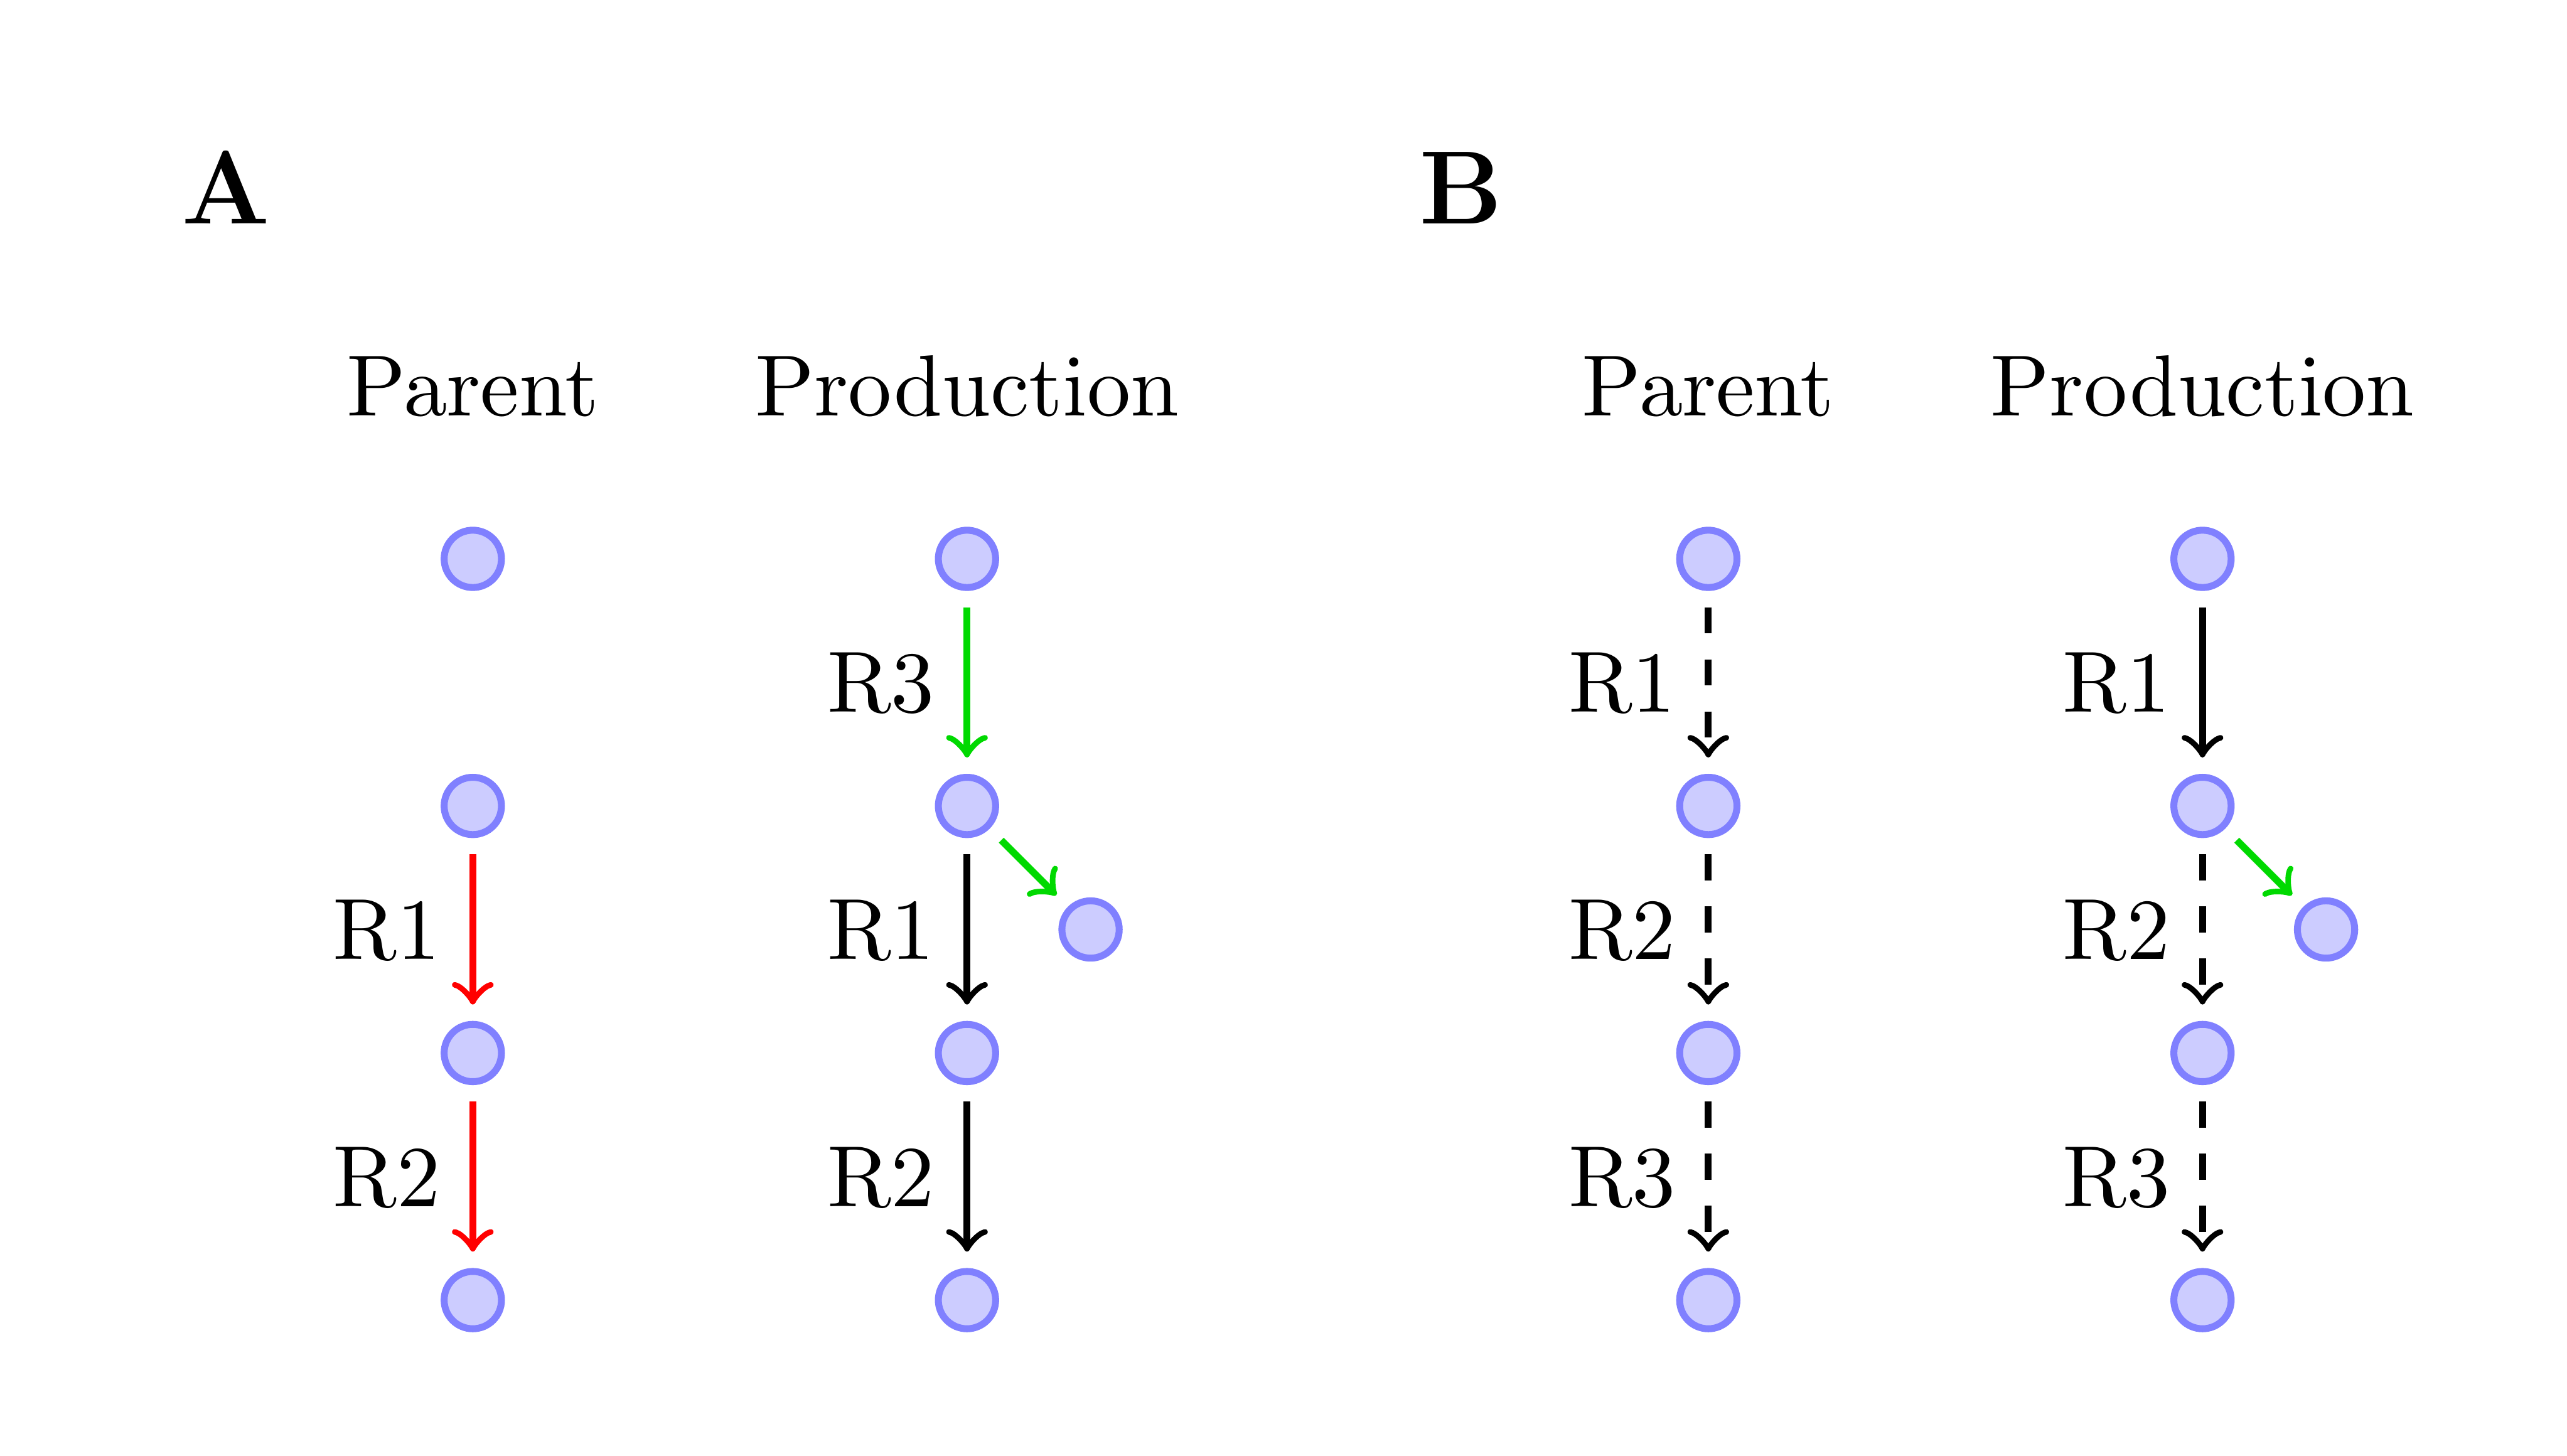
\includegraphics[width=.8\textwidth]{ms1-sm2-f1}
    \caption[Blocked and co-set reactions in deletion candidate determination]{(A.) Blocked reactions. The red arrows represent reactions originally blocked in the parent model, because the substrate of R1 cannot be produced. When heterologus reactions (green arrows) are added to produce a target chemical, the originally blocked reactions may become active and drain an intermediate of the production pathway. (B.) Reaction co-sets. The dashed arrows are used to indicated a fully correlated set. The addition of heterologous reactions (green arrows), alters the co-set definition and has important effect in deletion candidates. If R1 is considered as a deletion candidate, instead of R2 or R3, that would prevent the elimination of a potentially undesired pathway.}
\label{fig:candidaterxn}
\end{figure}

    %%%%%%%%%%%%%%%%%%%%%%%%%%%%%%%%%%%%%%%%%%%%%%%%%%%%%%%%%%%%%%%%%%%%%%%%%%%%%%%%%%%%%%%%%%%%%%%%%%%%%
    % A VITA IS REQUIRED
    %%%%%%%%%%%%%%%%%%%%%%%%%%%%%%%%%%%%%%%%%%%%%%%%%%%%%%%%%%%%%%%%%%%%%%%%%%%%%%%%%%%%%%%%%%%%%%%%%%%%%
    \addToTOC{Vita}
    \chapter*{Vita} \label{ch:vita}
Sergio Garcia is originally from Murcia, a southeastern region of Spain.
After finishing highschool, he began his studies in Chemical Engineering at the university of Murcia, founded in 1272 among the first universities in the world.
Although the Chemical Engineering program is only a few decades old.
Sergio spent his junior year abroad at the University of Tennesse Knoxville (UTK) throught the International Student Exchange Program scholarship, where he became involved in undegraduate research.
He then returned to finish his degree in Murcia, where he also pursued undegraduate research at the Department of Biochemistry and Molecular Biology.
After completion of his undegraduate degree, he returned to UTK to pursue a PhD in Chemical and Biomolecular Engineering.
In his free time, Sergio enjoys playing music, meditation, and cycling.
%Vita goes here. The vita should be a brief biography about the author written in third person and paragraph format. It should not be the author's resume or CV.

\end{document}
